% LaTeX source for textbook ``The Little Book of Semaphores, 2nd edition''
% Copyright 2016 Allen B. Downey.

% Permission is granted to copy, distribute and/or modify this
% document under the terms of the Creative Commons
% Attribution-NonCommercial-ShareAlike 4.0 International (CC BY-NC-SA 4.0)
% http://creativecommons.org/licenses/by-nc-sa/4.0/



\documentclass{book}

\usepackage[magyar]{babel}
\usepackage[utf8]{inputenc}
\usepackage{indentfirst}
\usepackage[T1]{fontenc}

\usepackage{fancyhdr}
\usepackage{listings}
\lstset{%
        inputencoding=utf8,
            extendedchars=true,
            literate=%
            {á}{{\'{a}}}1
            {é}{{\'{e}}}1
            {è}{{\`{e}}}1
            {ê}{{\^{e}}}1
            {ë}{{\¨{e}}}1
            {í}{{\'{i}}}1
            {ó}{{\'{o}}}1
            {ö}{{\"{o}}}1
            {ő}{{\H{o}}}1
            {ô}{{\^{o}}}1
            {ú}{{\'{u}}}1
            {ü}{{\"{u}}}1
            {ű}{{\H{u}}}1
            {û}{{\^{u}}}1
            {ù}{{\`{u}}}1
            {â}{{\^{a}}}1
            {à}{{\`{a}}}1
            {î}{{\^{i}}}1
            {ô}{{\^{o}}}1
            {ç}{{\c{c}}}1
            {Ç}{{\c{C}}}1
            {É}{{\'{E}}}1
            {Ê}{{\^{E}}}1
            {À}{{\`{A}}}1
            {Â}{{\^{A}}}1
            {Í}{{\'{I}}}1
            {Ü}{{\"{U}}}1
    }


\usepackage{graphicx}
\usepackage{color}
\usepackage{url}
\usepackage{makeidx}

\usepackage[colorlinks=true, linkcolor=blue, urlcolor=blue]{hyperref}

%\usepackage[printwatermark]{xwatermark}
%\usepackage{xcolor}
%\newwatermark*[allpages,angle=55,scale=2.5,xpos=0,ypos=0]{MUNKAPÉLDÁNY \\ NYELVI LEKTORRA VÁR \\ TOVÁBBADNI TILOS}

%\newwatermark[allpages,color=red!50,angle=45,scale=3,xpos=0,ypos=0]{MUNKAPÉLDÁNY\cr NYELVI LEKTORRA VÁR}
%\SetWatermarkText{MUNKAPÉLDÁNY\cr NYELVI LEKTORRA VÁR}

\title{Szemaforok kiskönyve}

\author{Allen B. Downey}

\newcommand{\theversion}{Version 2.2.1}

\sloppy

\newcommand{\clearemptydoublepage}{\newpage\cleardoublepage}
\newcommand{\blankpage}{\newpage}

\pagestyle{fancyplain}

\renewcommand{\chaptermark}[1]{\markboth{#1}{}}
\renewcommand{\sectionmark}[1]{\markright{\thesection\ #1}{}}

\lhead[\fancyplain{}{\bfseries\thepage}]%
      {\fancyplain{}{\bfseries\rightmark}}
\rhead[\fancyplain{}{\bfseries\leftmark}]%
      {\fancyplain{}{\bfseries\thepage}}
\cfoot{}

% Commands that control the appearance of the listings
\definecolor{light-gray}{gray}{0.95}

\lstset{basicstyle=\tt, frame=single, 
backgroundcolor=\color{light-gray}, escapeinside={(*}{*)},
numbers=left, numberstyle=\tiny, numbersep=10pt}

\makeindex

\begin{document}
\title {Szemaforok kiskönyve}
\author {Allen B. Downey}

\date {\theversion}
\maketitle

\vspace{2in}
\begin{center}
{\Large The Little Book of Semaphores}

Second Edition
\vspace{0.25in}

\theversion
\vspace{0.25in}

Copyright 2016 Allen B. Downey
\end{center}
\vspace{0.25in}

Permission is granted to copy, distribute and/or modify this
document under the terms of the Creative Commons
Attribution-NonCommercial-ShareAlike 4.0 International (CC BY-NC-SA 4.0)
at \url{http://creativecommons.org/licenses/by-nc-sa/4.0}.

The original form of this book is LaTeX source code.
Compiling this LaTeX source has the effect of generating
a device-independent representation of a book, which
can be converted to other formats and printed.

This book was typeset by the author using latex, dvips and ps2pdf,
among other free, open-source programs.
The LaTeX source for this book is available from
\url{http://greenteapress.com/semaphores}.

A magyar változatot a Pécsi Tudományegyetem Természettudományi Karának hallgatói és oktatói készítették.

Fordították:

Bodor András,
Hang Barnabás,
Kecskeméti Dávid,
Bagoly Dániel,
Futó Gábor,
Mózer Alexandra,
Illés Ádám,
Zádori József,
Váradi Róbert,
Csizmazia Marcell,
Riba Dániel,
Budavári Richárd,
Hegyi Bálint,
Schneider András,
Ladics Gábor,
Bruszt Barna,
Gradwohl Ádám,
Baranyai Csaba,
Drexler Ádám,
Tóth Norbert,
Pusztai Balázs,
Fehér András,
László Gábor,
Kulcsár Ákos.

Lektorálták:

Urbán Emese, Czigány Elliot, Sergiu Bolboaca, Ruff János.

Szerkesztette:

Bodor András.
\frontmatter

\chapter{Előszó}

Most undergraduate Operating Systems textbooks have a module on
Synchronization, which usually presents a set of primitives
(mutexes, semaphores, monitors, and sometimes condition variables),
and classical problems like readers-writers and
producers-consumers.

A legtöbb BsC szintű Operációs rendszerek tankönyvben van egy rész
a szinkronizációról, ahol általában szinkronizációs primitíveket
(kökiz\footnote{Mutex néven közismert}, szemafor, monitor, néha feltételváltozó) és klasszikus
problémákat (pl. írók-olvasók, termelők-fogyasztók)
ismertetnek.

When I took the Operating Systems class at Berkeley, and taught it at
Colby College, I got the impression that most students were able to
understand the solutions to these problems, but few would have been
able to produce them, or solve similar problems.

Amikor átvettem az Operációs rendszerek előadást a Berkeley-n, és amikor
tanítottam a Colby College-ben, az volt a benyomásom, hogy a legtöbb
diák érti ezen problémák megoldásait, de kevesen jöttek volna rá
maguktól, vagy tudtak volna megoldani hasonló problémákat.

One reason students don't understand this material deeply is that
it takes more time, and more practice, than most classes can spare.
Synchronization is just one of the modules competing for space in
an Operating Systems class, and I'm not sure I can argue that it is
the most important.  But I do think it is one of the most challenging,
interesting, and (done right) fun.

Az egyik oka annak, hogy a diákok ezt az anyagrészt nem értik
olyan mélyen az, hogy ennek elsajátítása több időt és gyakorlást igényel, mint
amennyit a legtöbb kurzus erre fordítani tud. A szinkronizáció
csupán az egyike az időért versengő moduloknak egy Operációs rendszerek
előadásban, és nem vagyok abban biztos, hogy tudnék amellett érvelni, hogy
ez a legfontosabb. De úgy gondolom, ez az egyik legtöbb kihívással rendelkező,
legérdekesebb, és -- ha jól oktatják -- a legszórakoztatóbb is.
 
I wrote the first edition this book with the goal of identifying
synchronization idioms and patterns that could be 
understood in isolation and then assembled to solve complex problems.
This was a challenge, because synchronization code doesn't compose
well; as the number of components increases, the number of interactions
grows unmanageably.

A köny első kiadását azzal a céllal írtam, hogy olyan szinkronizációs
alapproblémákat és mintázatokat azonosítsak, amiket önnállóan meg
lehet érteni, majd kombinálásukkal bonyolultabb problémákat lehet
megoldani. Ez egy komoly kihívás volt, mert a szinkronizáció
nagyon nehezen modularizálható. Ahogy a komponensek száma nő, úgy
a kölcsönhatások száma is kezelhetetlen mértékben nő.

Nevertheless, I found patterns in the solutions I saw, and discovered
at least some systematic approaches to assembling solutions that are
demonstrably correct.

Ennek ellenére találtam mintázatokat az általam látott megoldásokban,
és felfedeztem legalább néhány szisztematikus megközelítését az építőkövek
összerakásának, amikről belátható, hogy helyesek.

I had a chance to test this approach when I taught Operating Systems
at Wellesley College.  I used the first edition of {\em The Little
Book of Semaphores} along with one of the standard textbooks, and I
taught Synchronization as a concurrent thread for the duration of the
course.  Each week I gave the students a few pages from the book,
ending with a puzzle, and sometimes a hint.  I told them not to look
at the hint unless they were stumped.

Volt lehetőségem tesztelni ezt a megközelítést, amikor Operációs
rendszereket tanítottam a Wellesley College-ben. A {\em Szemaforok
kiskönyve} első kiadását használtam az egyik bevált tankönyv mellett,
és a szinkronizációt mint egy konkurens szálat tanítottam a kurzus
teljes ideje alatt. Minden héten kiadtam a könyv néhány oldalát a
hallgatóknak, ami egy rejtvénnyel vagy néha egy tippel végződött.
Azt mondtam nekik, hogy a segítséget csak akkor nézzék meg, ha végképp elakadtak.

I also gave them some tools for testing their solutions: a small
magnetic whiteboard where they could write code, and a stack of
magnets to represent the threads executing the code.

Ezen kívül adtam nekik eszközöket a megoldások kipróbálásához:
egy kis mágnestáblát, ahová a kódot írhatták, és táblamágneseket,
amikkel a szálak végrehajtását követhették nyomon.

The results were dramatic.  Given more time to absorb the material,
students demonstrated a depth of understanding I had not seen before.
More importantly, most of them were able to solve most of the puzzles.
In some cases they reinvented classical solutions; in other cases
they found creative new approaches.

A hatás drámai volt. Azzal, hogy több idő volt a tananyag elsajátítására,
a diákok olyan mélységben értették meg azt, amit korábban sosem láttam.
Ami még fontosabb: legtöbbjük önállóan meg tudta oldani a feladványok
többségét. Néha újra felfedezték a klasszikus megoldásokat, máskor
kreatív új megközelítéseket találtak.

When I moved to Olin College, I took the next step and created a
half-class, called Synchronization, which covered
{\em The Little Book of Semaphores} and also the implementation of
synchronization primitives in x86 Assembly Language, POSIX, and
Python.

Amikor Az Olin College-be mentem, egy lépéssel tovább mentem:
létrehoztam egy félkurzust Szinkronizáció címmel, ami a
{\em Szemaforok kiskönyvét} tartalmazta, és a szinkronizációs
primitívek megvalósítását x86-os assembly nyelven, POSIX-ban
és Python nyelven.

The students who took the class
helped me find errors in the first edition and several
of them contributed solutions that were better than mine.  At the
end of the semester, I asked each of them to write a new,
original problem (preferably with a solution).  I have added their
contributions to the second edition.

Az órán résztvevő hallgatókkal számos hibát javítottunk ki
az első kiadásból, és többen közülük találtak olyan megoldást,
amely jobb volt, mint az enyém. A félév végén megkértem őket,
hogy írjanak egy-egy új feladványt (lehetőleg megoldással együtt).
Ezeket feladványokat beletettem a második kiadásba.

Also since the first edition appeared, Kenneth Reek presented the
article ``Design Patterns for Semaphores'' at the ACM Special Interest
Group for Computer Science Education.  He presents a problem, which
I have cast as the Sushi Bar Problem, and two solutions that demonstrate
patterns he calls ``Pass the baton'' and ``I'll do it for you.''
Once I came to appreciate these patterns, I was able to apply them
to some of the problems from the first edition and produce solutions
that I think are better.

Az első kiadás megjelenése óta Kenneth Reek publikálta „Design Patterns for Semaphores”
című cikkét az ACM Special Interest Group for Computer Science Education-ön.
Bemutatott egy problémát, amit a könyvben a Szusi bár problémává
alakítottam, és két megoldást, amik az általa „add tovább a botot!”
és „majd én megcsinálom neked” nevű mintákat demonstrálják.
Miután megértettem ezeket a mintákat, tudtam őket alkalmazni
az első kiadás néhány feladatára, és olyan megoldásokat találni,
amelyek szerintem jobbak az eredetinél.

One other change in the second edition is the syntax.  After I wrote
the first edition, I learned Python, which is not only a great
programming language; it also makes a great pseudocode language.  So I
switched from the C-like syntax in the first edition to syntax
that is pretty close to executable Python\footnote{The primary
difference is that I sometimes use indentation to indicate code that
is protected by a mutex, which would cause syntax errors in Python.}.
In fact, I have written a simulator that can execute many of the
solutions in this book.

Egy másik változás az első kiadáshoz képest a szintaxis. Az első kiadás
megírása után megtanultam Pythonban programozni, ami nem csupán egy
remek programozási nyelv, de pszeudókódnak is kiváló. Úgyhogy
átálltam az első kiadás C-szerű szintaxisáról egy olyanra, ami
egész közel van a végrehajtható Pythonhoz.\footnote{A legfontosabb
különbség, hogy néha szövegbehúzást használok egy kökiz (mutex) által
védett kódrészlethez, ami az igazi Pythonban szintaktikus hibát okozna.}
Valójában írtam egy szimulátort, ami végre tudja hajtani a könyv
legtöbb megoldását.

Readers who are not familiar with Python will (I hope) find it mostly
obvious.  In cases where I use a Python-specific feature, I explain the
syntax and what it means.  I hope that these changes make the book
more readable.

A Pythonhoz nem értő olvasók is --remélem-- könnyen megértik a kódot.
Ahol valamilyen Python specifikus dolgot használok, külön elmagyarázom
a szintaxist és a jelentését. Remélem, ezek a változások sokkal olvashatóbbá
teszik a könyvet.

The pagination of this book might seem peculiar, but there is a method
to my whitespace.  After each puzzle, I leave enough space that the
hint appears on the next sheet of paper and the solution on the next
sheet after that.  When I use this book in my class, I hand it out a
few pages at a time, and students collect them in a binder.  My
pagination system makes it possible to hand out a problem without
giving away the hint or the solution.  Sometimes I fold and staple the
hint and hand it out along with the problem so that students can
decide whether and when to look at the hint.  If you print the book
single-sided, you can discard the blank pages and the system still
works.

A könyv laptördelése furcsának tűnhet, de van mögötte rendszer.
Minden feladvány után elég hely van, hogy a tipp a következő
új lapon jelenjen meg, a megoldás pedig megint új lapon.
Amikor órán használom a könyvet, egyszerre néhány oldalt osztok ki,
amiket a diákok lefűzve gyűjtenek. Az én laptördeléses rendszerem
lehetővé teszi, hogy úgy adjak ki problémákat, hogy közben nem adom
ki sem a tippeket, sem pedig a megoldásokat.
Néha viszont a tippet is kiadom a feladattal együtt, ilyenkor
a diákok eldönthetik, igénybe veszik-e, és
ha igen, mikor a segítséget. Aki egyoldalasan nyomtatja ki a könyvet,
elhagyhatja az üres oldalakat, a nélkül is működik a rendszer.

This is a Free Book, which means that anyone is welcome to read,
copy, modify and redistribute it, subject to the restrictions of the
license.  I hope that people
will find this book useful, but I also hope they will help continue
to develop it by sending in corrections, suggestions, and additional
material.  Thanks!

Ez egy szabad könyv, vagyis bárki elolvashatja, lemásolhatja, módosíthatja,
terjesztheti a licenszben lévő megkötésekkel. Remélem, az olvasók
hasznosnak találják a könyvet, de azt is remélem, hogy továbbra is
segítenek jobbá tenni a könyvet hibajelentések, javaslatok és
új feladatok küldésével. Köszönöm.

\vspace{0.3in}

\noindent Allen B. Downey \\
\noindent Needham, Massachusetts, Egyesült Államok \\
\noindent 2005. június 1. \\


\section*{Contributor's list}

The following are some of the people who have contributed to this
book:

\begin{itemize}

\item Many of the problems in this book are variations of classical
problems that appeared first in technical articles and then in textbooks.
Whenever I know the origin of a problem or solution, I acknowledge it
in the text.

\item I also thank the students at Wellesley College who worked with
the first edition of the book, and the students at Olin College who
worked with the second edition.

\item Se Won sent in a small but important correction in my presentation
of Tanenbaum's solution to the Dining Philosophers Problem.

\item Daniel Zingaro punched a hole in the Dancer's problem, which
provoked me to rewrite that section.  I can only hope that it makes more
sense now.  Daniel also pointed out an error in a previous version of
my solution to the H$_2$O problem, and then wrote back a year later
with some typos.

\item Thomas Hansen found a typo in the Cigarette smokers problem.

\item Pascal R\"{u}tten pointed out several typos, including my embarrassing
misspelling of Edsger Dijkstra.

\item Marcelo Johann pointed out an error in my solution to the
Dining Savages problem, and fixed it!

\item Roger Shipman sent a whole passel of corrections as well as
an interesting variation on the Barrier problem.

\item Jon Cass pointed out an omission in the discussion of dining
philosophers.

\item Krzysztof Ko\'{s}ciuszkiewicz sent in several corrections, including
a missing line in the Fifo class definition.

\item Fritz Vaandrager at the Radboud University Nijmegen in the
Netherlands and his students Marc Schoolderman, Manuel Stampe and Lars
Lockefeer used a tool called UPPAAL to check several of the solutions
in this book and found errors in my solutions to the Room Party problem
and the Modus Hall problem.

\item Eric Gorr pointed out an explanation in Chapter 3 that was
not exactly right.

\item Jouni Lepp\"{a}j\"{a}rvi helped clarify the origins of semaphores.

\item Christoph Bartoschek found an error in a solution to
the exclusive dance problem.

\item Eus found a typo in Chapter 3.

\item Tak-Shing Chan found an out-of-bounds error in {\tt counter\_mutex.c}.

\item Roman V. Kiseliov made several suggestions for improving
the appearance of the book, and helped me with some \LaTeX~issues.

\item Alejandro C\'{e}spedes is working on the Spanish translation of this
book and found some typos.

\item Erich Nahum found a problem in my adaptation of Kenneth Reek's
  solution to the Sushi Bar Problem.

\item Martin Storsj\"{o} sent a correction to the generalized smokers problem.

\item Cris Hawkins pointed out an unused variable.

\item Adolfo Di Mare found the missing ``and''.

\item Simon Ellis found a typo.

\item Benjamin Nash found a typo, an error in one solution, and
a malfeature in another.

\item Alejandro Pulver found a problem with the Barbershop solution.

\end{itemize}

% endcontrib

\tableofcontents
\clearemptydoublepage

\mainmatter


\chapter{Bevezetés}

\section{Szinkronizáció}
\label{synch}

In common use, ``synchronization'' means making two things happen
at the same time.  In computer systems, synchronization is a little
more general; it refers to relationships among events---any number
of events, and any kind of relationship (before, during, after).

Mindennapi értelemben a „szinkronizáció” azt jelenti: gondoskodunk
arról, hogy két dolog egyszerre következzen be. A számítástudományban
a szinkronizációnak kissé általánosabb a jelentése: események
időbeli viszonyait jelenti -- akárhány esemény akármilyen viszonyát
(előtte, alatta, utána).

Computer programmers are often concerned with {\bf synchronization
constraints}, which are requirements pertaining to the order of
events.  Examples include:

A programozók gyakran {\bf szinkronizációs megszorításokkal} foglalkoznak,
amik események sorrendiségére szabnak ki feltételeket. Például:

\begin{description}

\item[Serialization:] Event A must happen before Event B.

\item[Mutual exclusion:] Events A and B must not happen at the same time.

\end{description}

\begin{description}

\item[Szerializáció:] A eseménynek B esemény előtt kell lezajlania.

\item[Kölcsönös kizárás:] A és B esemény nem következhet be egyszerre.

\end{description}

In real life we often check and enforce synchronization constraints 
using a clock.  How do we know if A happened before B?  If we
know what time both events occurred, we can just compare the times.

A való életben a szinkronizációs megszorításokat gyakran egy óra
segítségével ellenőrizzük és tartatjuk be. Honnan tudjuk, hogy A
esemény B előtt történt? Ha tudjuk, melyik mikor történt, csak
összehasonlítjuk az időpontokat.

In computer systems, we often need to satisfy synchronization
constraints without the benefit of a clock, either because there
is no universal clock, or because we don't know with fine enough
resolution when events occur.

Számítógépes rendszerekben gyakran egy óra segítsége nélkül kell
betartatni szinkronizációs megszorításokat, vagy azért, mert
egy univerzális óra nem létezik, vagy azért, mert nem tudjuk
elegendő pontossággal, mikor történnek az események.

That's what this book is about: software techniques for enforcing
synchronization constraints.

Erről szól ez a könyv: szoftver technikák szinkronizációs megszorítások
betartatására.

\section{Számítási modell}

In order to understand software synchronization, you have to
have a model of how computer programs run.  In the simplest
model, computers execute one instruction after another in
sequence.  In this model, synchronization is trivial; we can
tell the order of events by looking at the program.  If Statement
A comes before Statement B, it will be executed first.

Ahhoz, hogy megértsük a szoftver szinkronizációt, kell, hogy legyen
egy modellünk arról, hogyan fut egy számítógépprogram. A legegyszerűbb
modellben a számítógépek sorrendben egymás után egyesével
hajtják végre az utasításokat. Ebben a modellben a szinkronizáció
triviális. Meg tudjuk mondani az utasítások sorrendjét a programkód
alapján. Ha az A utasítás előbb van a programban, mint a B utasítás,
akkor az lesz előbb végrehajtva.

There are two ways things get more complicated.  One possibility
is that the computer is parallel, meaning that it has multiple
processors running at the same time.  In that case it is not easy
to know if a statement on one processor is executed before a
statement on another.

Két módon lehet elbonyolítani a dolgokat. Az egyik lehetőség, hogy
a számítógépunk párhuzamos, vagyis több processzor is fut benne
egyidőben. Ebben az esetben nem könnyű megmondani, hogy egy
utasítás az egyik processzoron előbb lesz-e végrehajtva, mint
egy másik egy másik processzoron.

Another possibility is that a single processor is running multiple
threads of execution.  A thread is a sequence of instructions
that execute sequentially.  If there are multiple threads, then
the processor can work on one for a while, then switch to
another, and so on.

A másik lehetőség, hogy egyetlen processzor több végrehajtási
szálat is futtat. Egy szál az utasítások sorozata, amik
szekvenciálisan (sorrendben egymás után) lesznek végrehajtva.
Ha több szál van, a pocesszor dolgozhat az egyiken egy ideig, aztán
átválthat egy másikra, és így tovább.

In general the programmer has no control over when each thread runs;
the operating system (specifically, the scheduler) makes those
decisions.  As a result, again, the programmer can't tell when
statements in different threads will be executed.

Általában a programozónak nincs beleszólása abba, mikor melyik
szál fusson. Erről az operációs rendszer (azon belül az ütemező)
dönt. Ennek eredményeként a programozó nem tudhatja előre,
hogy a különböző szálak utasításai milyen sorrendben fognak végrehajtódni.

For purposes of synchronization, there is no difference between the
parallel model and the multithread model.  The issue is the
same---within one processor (or one thread) we know the order of
execution, but between processors (or threads) it is impossible to
tell.

A szinkronizáció szempontjából nincs különbség a párhuzamos és a
többszálas modell között. A probléma ugyanaz: egy processzoron (vagy
szálon) belül ismerjük a végrehajtási sorrendet, de processzorok
(vagy szálak) között ezt lehetetlen megtudni.

A real world example might make this clearer.  Imagine that you and
your friend Bob live in different cities, and one day, around dinner
time, you start to wonder who ate lunch first that day, you or Bob.
How would you find out?

Egy való életből vett példa segíthet ezt tisztázni. Tegyük fel,
hogy az Olvasó, és barátja Bob két különböző városban lakik, és
egy nap vacsora közben, azon kezdesz töprengeni, melyikőjük ebédelt
korábban, ő vagy Bob.

Obviously you could call him and ask what time he ate lunch.  But what
if you started lunch at 11:59 by your clock and Bob started lunch at
12:01 by his clock?  Can you be sure who started first?  Unless you
are both very careful to keep accurate clocks, you can't.

A legkézenfekvőbb dolog felhívni Bobot, és megkérdezni, hánykor
ebédelt. De mi van, ha az Olvasó 11:59-kor, Bob pedig 12:01-kor
kezdett bele az ebédbe? Tudhatjuk, hogy ki kezdte előbb? Hacsak
mindketten kínosan nem ügyelnek arra, hogy pontosan járjon az órájuk,
akkor ez lehetetlen.

Computer systems face the same problem because, even though their
clocks are usually accurate, there is always a limit to their
precision.  In addition, most of the time the computer does not keep
track of what time things happen.  There are just too many things
happening, too fast, to record the exact time of everything.

A számitógépes rendszerek hasonló problémával küszködnek, ugyanis,
bár az órájuk általában pontos, mindig van egy határa ennek a
pontosságnak. Ezen kívül, az idő legnagyobb részében a számítógép
nem tartja nyilván, hogy mi mikor történik. Egyszerűen túl sok minden
történik nagyon gyorsan ahhoz, hogy mindennek nyilvántartsák a pontos
idejét.

Puzzle: Assuming that Bob is willing to follow simple instructions, is
there any way you can {\em guarantee} that tomorrow you will eat lunch
before Bob?

Rejtvény: Feltételezve, hogy Bob hajlandó egyszerű utasításokat betartani,
hogyan lehetne {\em garantálni}, hogy másnap az Olvasó előbb ebédeljen, mint Bob?
 
\clearemptydoublepage
\section{Szerializáció üzenetekkel}
\label{serialization}

One solution is to instruct Bob not to eat lunch until you call.
Then, make sure you don't call until after lunch.  This approach may
seem trivial, but the underlying idea, message passing, is a real
solution for many synchronization problems.
At the risk of belaboring the obvious, consider this timeline.

Egy megoldás arra utasítani Bobot, hogy ne ebédeljen, amíg fel nem hívod.
Majd ügyelni arra, hogy csak azután hívd, ha már megebédeltél.
Ez a megközelítés triviálisnak tűnhet, de a mögötte meghúzódó ötlet
-- az üzenetküldés -- a szinkronizációs problémák egyik valódi megoldása.
Megkockáztatva, hogy fölöslegesen fogyasztjuk a tintát, tekintsük
az alábbi időbeosztásokat:

%
\begin{minipage}[t]{2in}
\begin{lstlisting}[title={„A” szál (Olvasó)}]{}
Reggelizz!
Dolgozz!
Ebédelj!
Hívd fel Bobot!
\end{lstlisting}
\end{minipage}
\hfill
\begin{minipage}[t]{2in}
\begin{lstlisting}[title={„B” szál (Bob)}]{}
Reggelizz!
Várj, amíg hívnak!
Ebédelj!
\end{lstlisting}
\end{minipage}
%
The first column is a list of actions you perform; in other words,
your thread of execution.  The second column is Bob's thread of
execution.  Within a thread, we can always tell what order things
happen.  We can denote the order of events

Az első oszlop az Olvasó által végrehajtott cselekedetek listája,
más szóval az Olvasó szála. A második oszlop Bob végrehajtási szála.
Egy szálon belül mindig meg tudjuk mondani, milyen sorrendben történnek
a dolgok. Jelölhetjük az események sorrendjét így:

%
\begin{eqnarray*}
o_1 < o_2 < o_3 < o_4  \\
b_1 < b_2 < b_3
\end{eqnarray*}
%
where the relation $a1 < a2$ means that a1 happened before a2.

ahol $o_1 < o_2$ azt jelenti, $o_1$ $o_2$ előtt történt.

In general, though, there is no way to compare events from different
threads; for example, we have no idea who ate breakfast first (is $a1
< b1$?).

Általában viszont semmiképpen sem tudjuk összehasonlítani különböző
szálak eseményeit. Például fogalmunk sincs, hogy ki reggelizett
hamarabb (vajon $o_1<b1$?).

But with message passing (the phone call) we {\em can} tell who ate
lunch first ($a3 < b3$).  Assuming that Bob has no other friends, he
won't get a call until you call, so $b2 > a4$ .  Combining all the
relations, we get

De az üzenetküldéssel (a telefonhívással) {\em meg tudjuk mondani},
ki ebédelt először ($o_3 < b_3$). Feltéve, hogy Bobnak nincs más
barátja nem fogják felhívni azelőtt, hogy az Olvasó hívná, vagyis
$b_2 > o_4$. Az összes relációt figyelembe véve:
%
\begin{eqnarray*}
b_3 > b_2 > a_4 > a_3
\end{eqnarray*}
%
which proves that you had lunch before Bob.

ami bizonyítja, hogy az Olvasó Bob előtt ebédelt.

In this case, we would say that you and Bob ate lunch
{\bf sequentially}, because we know the order of events, and you
ate breakfast {\bf concurrently}, because we don't.

Ebben az esetben azt mondhatjuk, az Olvasó és Bob {\bf szekvenciálisan}
ebédelt, mert az események sorrendje ismert, és {\bf konkurens módon}
reggelizett, mert a sorrend ismeretlen.

When we talk about concurrent events, it is tempting to say
that they happen at the same time, or simultaneously.  As a
shorthand, that's fine, as long as you remember the strict
definition:

Amikor konkurens eseményekről beszélünk, csábító azt mondani,
azok ugyanabban az időben, vagy szimultán történnek. Ez
elfogadható, mint egy rövidítés, de észben kell tartanunk
a pontos definíciót:

\begin{quote}
Two events are concurrent if we cannot tell by looking at
the program which will happen first.

Két esemény konkurens (konkurens módon történik), ha
a program kódja alapján nem lehet megmondani, melyik
következik be előbb.
\end{quote}

Sometimes we can tell, after the program runs, which happened first,
but often not, and even if we can, there is no guarantee that we will
get the same result the next time.

Néha a sorrend kiderül a program futása után, de gyakran nem, és
semmi garancia nincs arra, hogy legközelebb is ugyanazt a sorrendet kapjuk.

\newpage
\section{Nemdeterminizmus}

Concurrent programs are often {\bf non-deterministic}, which means it
is not possible to tell, by looking at the program, what will happen
when it executes.  Here is a simple example of a
non-deterministic program:

A konkurens programok gyakran {\bf nemdeterminisztikusak}, ami azt
jelenti, a programkód alapján lehetetlen megmondani, hogy mi fog
történni, amikor fut. Itt van egy egyszerű példa nemdeterminisztikus
programra:
 
\begin{minipage}[t]{2in}
\begin{lstlisting}[title={„A” szál}]{}
print("igen")
\end{lstlisting}
\end{minipage}
\hfill
\begin{minipage}[t]{2in}
\begin{lstlisting}[title={„B” szál}]{}
print("nem")
\end{lstlisting}
\end{minipage}

Because the two threads run concurrently, the order of
execution depends on the scheduler.  During any given run
of this program, the output might be ``yes no'' or ``no yes''.

Mivel a két szál konkurensen fut, a végrehajtási sorrend
az ütemezőtől függ. Egy adott futás alatt a kimenet lehet
„igen nem” vagy „nem igen” is.
 
Non-determinism is one of the things that makes concurrent
programs hard to debug.  A program might work correctly
1000 times in a row, and then crash on the 1001st run, depending
on the particular decisions of the scheduler.

A nemdeterminizmus az egyik dolog, amiért a konkurens
programoknál nehéz a hibakeresés. A program jól működhet
ezerszer egyhuzamban, aztán lefagyhat az 1001. alkalommal
az ütemező valamilyen döntése miatt.

These kinds of bugs are almost impossible to find by testing;
they can only be avoided by careful programming.

Az ilyen hibákat szinte lehetetlen teszteléssel megtalálni.
Csak figyelmes programtervezéssel lehet elkerülni.

\section{Megosztott változók}
\label{shared}

Most of the time, most variables in most threads are {\bf local},
meaning that they belong to a single thread and no other threads
can access them.  As long as that's true, there tend to be few
synchronization problems, because threads just don't interact.

Legtöbbször a legtöbb szál legtöbb változója {\bf lokális}, vagyis
egyetlen szálhoz tartozik, és más szálak nem férhetnek hozzá.
Amíg ez így van, általában kevés szinkronizációs probléma
szokott előfordulni, mert a szálak nem lépnek kölcsönhatásba.

But usually some variables are {\bf shared} among two or more
threads; this is one of the ways threads interact with each other.
For example, one way to communicate information between threads is
for one thread to read a value written by another thread.

De általában néhány változó {\bf megosztott} két vagy több szál
között, ez egy módja annak, ahogy a szálak kölcsönhathatnak
egymással. Az információátadás egyik módja például, hogy
az egyik szál kiolvas egy másik szál által beírt értéket.

If the threads are unsynchronized, then we cannot tell by looking at
the program whether the reader will see the value the writer writes
or an old value that was already there.
Thus many applications enforce the constraint that the reader
should not read until after the writer writes.  This is exactly
the serialization problem in Section~\ref{serialization}.

Ha a szálak nincsenek szinkronizálva, akkor nem tudjuk megmondani
a programkód alapján, vajon az olvasó az író által beírt értéket
fogja látni, vagy a régi értéket, ami ott volt.
Tehát sok alkalmazás megköveteli azt a feltételt, hogy az
olvasó nem olvashat addig, amíg az író be nem fejezte az írást.
Ez pontosan \aref{serialization}~fejezetben látott szerializációs
feladat.

Other ways that threads interact are
concurrent writes (two or more writers) and concurrent updates
(two or more threads performing a read followed by a write).
The next two sections deal with these interactions.  The other
possible use of a shared variable, concurrent
reads, does not generally create a synchronization problem.

A szálak kölcsönhatásának egyéb módjai: konkurens írások
(kettő vagy több írás) és konkurens frissítések (kettő vagy
több szál olvas, majd felülír). A következő két szakasz ezekkel
foglalkozik. A megosztott változók negyedik lehetséges használati
mintázata -- konkurens olvasás -- általában nem okoz szinkronizációs
problémát.
 
\subsection{Konkurens írások}

In the following example, {\tt x} is a shared variable accessed
by two writers.

A következő példában {\tt x} egy megosztott változó, amihez
két író szál fér hozzá.

\begin{minipage}[t]{2in}
\begin{lstlisting}[title={„A” szál}]{}
x = 5
print(x)
\end{lstlisting}
\end{minipage}
\hfill
\begin{minipage}[t]{2in}
\begin{lstlisting}[title={„B” szál}]{}
x = 7
\end{lstlisting}
\end{minipage}

What value of {\tt x} gets printed?  What is the final value of {\tt
x} when all these statements have executed?  It depends on the order
in which the statements are executed, called the {\bf execution path}.
One possible path is $a1 < a2 < b1$, in which case the output of the
program is {\tt 5}, but the final value is {\tt 7}.

{\tt x} milyen értéke lesz kiírva? Mi lesz {\tt x} végső értéke
a fenti utasítások lefutása után? Ez függ az utasítások végrehajtási
sorrendjétől, amit {\bf végrehajtási útnak} hívunk. Egy lehetséges
út $a1 < a2 < b1$, ebben az esetben a program kimenete {\tt 5}, de
a végső érték {\tt 7}.

Puzzle: What path yields output {\tt 5} and final
value {\tt 5}?

Rejtvény: Milyen út ad kimenetnek és végső értéknek
is {\tt 5}-öt?

Puzzle: What path yields output {\tt 7} and final
value {\tt 7}?

Rejtvény: Milyen út ad kimenetnek és végső értéknek
is {\tt 7}-et?

Puzzle: Is there a path that yields output {\tt 7} and final
value {\tt 5}?  Can you prove it?

Rejtvény: Van olyan út, ami kimenetnek {\tt 7}-et, végső értéknek
{\tt 5}-öt ad? Be tudod bizonyítani?

Answering questions like these is an important part of concurrent
programming:  What paths are possible and what are the
possible effects?  Can we prove that a given (desirable) effect is
necessary or that an (undesirable) effect is impossible?

Az ehhez hasonló kérdések megválaszolása nagyon fontos része
a konkurens programozásank. Milyen végrehajtási utak lehetségesek,
mik azok lehetséges hatásai? Be tudjuk-e bizonyítani, hogy egy
bizonyos (kívánatos) hatás bekövezte elkerülhetetlen, vagy
hogy egy nem kívánatosé lehetetlen?

\subsection{Konkurens frissítések}

An update is an operation that reads the value of a variable, computes
a new value based on the old value, and writes the new value.
The most common kind of update is an increment, in which the
new value is the old value plus one.  The following example
shows a shared variable, {\tt count}, being updated concurrently
by two threads.

A frissítés egy olyan művelet, ami kiolvas egy változót, kiszámol
egy új értéket a régi alapján, majd felülírja a változó régi értékét
az újjal. A leggyakoribb frissítésfajta az inkrementálás (eggyel növelés),
amikor az új érték egyenlő a régi érték plusz eggyel. Az alábbi példában egy
megosztott változót {\tt darab} két szál konkurens módon frissít.

\begin{minipage}[t]{2in}
\begin{lstlisting}[title={„A” szál}]{}
darab = darab + 1
\end{lstlisting}
\end{minipage}
\hfill
\begin{minipage}[t]{2in}
\begin{lstlisting}[title={„B” szál}]{}
darab = darab + 1
\end{lstlisting}
\end{minipage}

At first glance, it is not obvious that there is a synchronization
problem here.  There are only two execution paths, and they
yield the same result.

Első ránézésre nem nyilvánvaló, hogy a kódban egy szinkronizációs probléma
lapul. Csak két végrehajtási út van, és mindkettő ugyanaz az eredményt
adja.

The problem is that these operations are translated into
machine language before execution, and in machine language
the update takes two steps, a read and a write.
The problem is more obvious if we rewrite the code with a temporary
variable, {\tt temp}.

A probléma az, hogy ezeket a műveleteket gépi kódra fordítják
végrehajtás előtt, és gépi kódban a frissítés két utasításból
áll, egy olvasásból és egy írásból.

\begin{minipage}[t]{2in}
\begin{lstlisting}[title={„A” szál}]{}
temp = darab
darab = temp + 1
\end{lstlisting}
\end{minipage}
\hfill
\begin{minipage}[t]{2in}
\begin{lstlisting}[title={„B” szál}]{}
temp = darab
darab = temp + 1
\end{lstlisting}
\end{minipage}

(Ahol {\tt temp} szálra lokális változó, vagyis
kettő van belőle, szálanként egy.)

Now consider the following execution path 

Most tekintsük az alábbi végrehajtási utat:

\[  a1 < b1 < b2 < a2  \]

Assuming that the
initial value of {\tt x} is {\tt 0},
what is its final value?  Because
both threads read the same initial value, they write
the same value.  The variable is only incremented once, which
is probably not what the programmer had in mind.

Feltéve, hogy {\tt darab} kezdeti értéke {\tt 0},
mi lesz a végső értéke? Mivel mindkét szál ugyanazt az értéket
olvassa ki, ugyanazt is fogja visszaírni. A változó csak
egyszer lesz inkrementálva, és valószínűleg a programozó nem
ezt akarta.

This kind of problem is subtle because it is not always possible to
tell, looking at a high-level program, which operations are
performed in a single step and which can be interrupted.
In fact, some computers provide an increment instruction that
is implemented in hardware and cannot be interrupted.
An operation that cannot be interrupted is said to be
{\bf atomic}.

Az ilyen típusú problémák rendkívül körmönfontak, ugyanis
egy magasszintű programnyelven írt programban nem mindig
lehet megállapítani, hogy mely utasítások hajtódnak végre
egy lépésben, és melyeket lehet félbeszakítani. Valójában
bizonyos számítógépek rendelkeznek egy inkrementálás
utasítással, amit a hardwerbe van beépítve, és nem lehet
megszakítani. A megszakíthatatlan utasításokat {\bf atomi
utasításoknak} nevezzük.

So how can we write concurrent programs if we don't know which
operations are atomic?  One possibility is to collect specific
information about each operation on each hardware platform.
The drawbacks of this approach are obvious.

Hogyan lehet akkor konkurens programokat írni, ha nem tudjuk,
mely utasítások atomiak? Egy lehetőség, hogy minden lehetséges hardver
platformról begyűjtjük a szükséges információkat. Ennek a
megközelítésnek a hátrányai nyilvánvalóak.

The most common alternative is to make the conservative
assumption that all updates and all writes are not atomic,
and to use synchronization constraints to control concurrent
access to shared variables.

A legelterjedtebb alternatíva az, hogy konzervatív módon
azt tételezzük fel, hogy az írások és frissítések nem atomiak,
és szinkronizációs megszorításokkal szabályozzuk a megosztott
változókhoz való hozzáférést.

The most common constraint is mutual exclusion, or mutex,
which I mentioned in Section~\ref{synch}.  Mutual exclusion guarantees
that only one thread accesses a shared variable at a time,
eliminating the kinds of synchronization errors in this section.

A leggyakoribb megszorítás a kölcsönös kizárás, vagy kökiz (mutex),
amit már említettem \aref{synch}~fejezetben. A kölcsönös kizárás
garantálja, hogy egyszerre csak egy szál férjen hozzá egy megosztott
változóhoz, ezzel kiküszöböli az ebben a fejezetben látottakhoz hasonló
szinkronizációs hibákat.

Puzzle: Suppose that 100 threads run the following program concurrently
(if you are not familiar with Python, the {\tt for} loop runs the update
100 times.):

Rejtvény: Tegyük fel, hogy 100 szál futtatja konkurensen az alábbi
programot. (Ha valaki nem ismeri a Python nyelvet: a {\tt for} ciklus
százszor futtatja frissítést.)

\begin{lstlisting}[]{}
for i in range(100):
    temp = darab
    darab = temp + 1
\end{lstlisting}

What is the largest possible value of {\tt count} after all threads
have completed?  What is the smallest possible value?

Mi {\tt darab} legnagyobb lehetséges értéke, miután az összes szál lefutott?
Mi a legkisebb lehetséges értéke?

Hint: the first question is easy; the second is not.

Tipp: az első kérdés könnyű, a második nem.

\subsection{Kölcsönös kizárás üzenetekkel}

Like serialization, mutual exclusion
can be implemented using message passing.  For example, imagine that
you and Bob operate a nuclear reactor that you monitor from remote
stations.  Most of the time, both of you are watching for warning
lights, but you are both allowed to take a break for lunch.  It
doesn't matter who eats lunch first, but it is very important that
you don't eat lunch at the same time, leaving the reactor unwatched!

Ahogy a szerializáció, a kölcsönös kizárás is megvalósítható
üzenetküldésekkel. Például képzeljük el, hogy Bob és te egy
atomreakort felügyeltek távoli munkaállomásokról. Az idő túlnyomó többségében
mindketten figyelitek, nem gyullad-e ki egy figyelmeztető lámpa,
de mindketten elmehettek ebédelni. Mindegy, hogy ki ebédel először,
de nagyon fontos, hogy ne ebédeljetek egyszerre, mert akkor felügyelet
nélkül marad a reaktor.

Puzzle: Figure out a system of message passing (phone calls) that
enforces these restraints.  Assume there are no clocks, and you
cannot predict when lunch will start or how long it will last.  What
is the minimum number of messages that is required?

Rejtvény: Találjunk egy üzenetküldéses (telefonálós) módszert,
ami biztosítja a fenti feltételeket. Bár egy atomreaktorról
van szó, tételezzük fel, hogy nincsenek órák, és nem lehet
előre megmondani, mikor támad valakinek ebédelhetnékje,
vagy mennyi ideig fog ebédelni. Legalább hány üzenet szükséges?

\clearemptydoublepage
\chapter{Szemaforok}

In real life a semaphore is a system of signals used to communicate
visually, usually with flags, lights, or some other mechanism.  In
software, a semaphore is a data structure that is useful for solving a
variety of synchronization problems.

A való életben a szemafor egy jelzésrendszer amit vizuális kommunikációban
használunk, általában zászlókkal , fényekkel, vagy valamilyen más mechanizmussal.
A szoftverekben a szemafor egy adatstruktúra ami hasznos rengeteg
szinkronizációs probléma megoldásában.

Semaphores were invented by Edsger Dijkstra, a famously eccentric
computer scientist.  Some of the details have changed since the
original design, but the basic idea is the same.

A szemaforokat Edgser Dijkstra,
a különcként elhíresült számítógép tudós találta fel. Sok részlet
változott a kezdeti felépítését\H{o}l, de az alap elképzelés ugyan
az maradt.

\section{Definíció}

A semaphore is like an integer, with three differences:

\begin{enumerate}

\item When you create the semaphore, you can initialize its value to
any integer, but after that the only operations you are allowed to
perform are increment (increase by one) and decrement (decrease by
one).  You cannot read the current value of the semaphore.

\item When a thread decrements the semaphore, if the result is
negative, the thread blocks itself and cannot continue until another
thread increments the semaphore.

\item When a thread increments the semaphore, if there are other
threads waiting, one of the waiting threads gets unblocked.

\end{enumerate}

A szemafor olyan mint egy integer, 3 különbséggel:

\begin{enumerate}

\item Amikor létrehozzuk a szemafort, akkor az értékét egy integerként inicializáljuk
de utána már csak az inkrementálás (egyel való növelés) és dekrementálás
(egyel való csökkentés) műveletek engedélyezettek. Az aktuális
érték nem olvasható ki a szemaforból.

\item Ha egy szál dekrementálja a szemafort, és a szemafor
értéke negatív lesz, a szál blokkolja magát és a végrehajtása nem
folytatódhat addig, amíg egy másik szál nem inkrementálja a szemafort.

\item Ha egy szál inkrementálja a szemafort, és vannak várakozó szálak, akkor a várakozók
közül az egyik blokkolása feloldódik.

\end{enumerate}

To say that a thread blocks itself (or simply ``blocks'') is to say
that it notifies the scheduler that it cannot proceed.  The scheduler
will prevent the thread from running until an event occurs that causes
the thread to become unblocked.  In the tradition of mixed metaphors
in computer science, unblocking is often called ``waking''.


That's all there is to the definition, but there are some
consequences of the definition you might want to think about.

Ha azt mondjuk, egy szál blokkolja magát, az azt jelenti, hogy értesíti az ütemezőt,
hogy nem tud tovább folytatódni. Az ütemező nem fogja engedni
futni, amíg valamilyen esemény következtében a szál blokkolása fel nem oldódik.
A feloldást gyakran „ébresztésnek” is hívjuk.

Ennyit kell definiálnunk de van pár következménye a definícióknak
amiket érdemes átgondolni.

\begin{itemize}

\item In general, there is no way to know before a thread decrements a
semaphore whether it will block or not (in specific cases you might
be able to prove that it will or will not).

\item After a thread increments a semaphore and another thread gets
woken up, both threads continue running concurrently.  There is no way
to know which thread, if either, will continue immediately.

\item When you signal a semaphore, you don't necessarily know whether
another thread is waiting, so the number of unblocked threads may
be zero or one.

\end{itemize}

\begin{itemize}

\item Általánosságban elmondhatjuk, hogy nem tudjuk, hogy ha egy szál dekrementálja
a szemafort akkor blokkolni fog vagy sem (speciális esetekben meg
lehet bizonyosodni róla, hogy fog-e blokkolni vagy nem).

\item Miután egy szál inkrementálja a szemafort és egy másik szál felébred, mindkét
szál konkurens módon folytatja a futást. Nem lehet megmondani, hogy
közülük melyik szál (talán egyik sem) fog folytatódni azonnal.

\item Amikor jelzünk a szemafornak (az inkrementálás másik elnevezése),
nem feltétlenül tudjuk, hogy várakozik-e más szál, szóval a felébresztett
szálak száma lehet 0 vagy 1.

\end{itemize}

Finally, you might want to think about what the value of the
semaphore means.  If the value is positive, then it represents the
number of threads that can decrement without blocking.  If it
is negative, then it represents the number of threads that have
blocked and are waiting.  If the value is zero, it means there
are no threads waiting, but if a thread tries to decrement, it
will block.

Végezetül érdemes belegondolni, hogy mit is jelent a szemafor értéke.
Ha az értéke pozitív, akkor ez reprezentálja a szálak számát, amik dekrementálhatnak
blokkolás nélkül. Ha negatív, akkor azoknak a szálaknak a számát reprezentálja,
amiket blokkoltak és várakoznak. Ha az értéke 0, az azt jelenti, hogy
nincsenek várakozó szálak, de ha egy szál megpróbál dekrementálni, akkor
blokkolni fog.

\section{Szintaxis}

In most programming environments, an implementation of semaphores is
available as part of the programming language or the operating system.
Different implementations sometimes offer slightly different
capabilities, and usually require different syntax.

In this book I will use a simple pseudo-language to demonstrate
how semaphores work.  The syntax for creating a new semaphore
and initializing it is

A legtöbb fejlesztési környezetben, a szemaforok valamilyen implementációja
elérhető a programozási nyelvből vagy az operációs rendszerből.
Különböző implementációk kicsit más lehetőségekkel szolgálnak
és általában különbözik a szintaxisuk.

Ebben a könyvben egy egyszerű
pszeudó nyelvet fogok használni a szemaforok demonstrálásához. A kód,
amivel létrehozunk és iniciálunk egy szemafort a következő:
%
\begin{lstlisting}[title={Szemafor inicializálás szintaxisa}]{}
fred = Szemafor(1)
\end{lstlisting}
%
The function {\tt Semaphore} is a constructor; it creates and
returns a new Semaphore.  The initial value of the semaphore
is passed as a parameter to the constructor.

The semaphore operations go by different names in different environments.
The most common alternatives are

A {\tt Szemafor} függvény egy konstruktor, létrehoz és visszaad egy új
szemafort. A szemafor kezdő értékét paraméterként adjuk át a
konstruktorban.

A szemafor műveleteinek különböző nevük van különböző
környezetekben. A leggyakoribbak:
%
\begin{lstlisting}[title={Szemafor műveletek}]{}
fred.increment()
fred.decrement()	
\end{lstlisting}
%
és
%
\begin{lstlisting}[title={Szemafor műveletek}]{}
fred.signal()
fred.wait()	
\end{lstlisting}
%
és
%
\begin{lstlisting}[title={Szemafor műveletek}]{}
fred.V()
fred.P()	
\end{lstlisting}
%
It may be surprising that there are so many names, but there is a
reason.  {\tt increment} and {\tt decrement}
describe what the operations {\em do}.  {\tt signal} and {\tt wait}
describe what they are often {\em used for}.  And {\tt V} and {\tt P} were
the original names proposed by Dijkstra, who wisely realized that a
meaningless name is better than a misleading name\footnote{If you speak
Dutch, {\tt V} and {\tt P} aren't completely meaningless.}.

I consider the other pairs misleading because {\tt increment} and {\tt
decrement} neglect to mention the possibility of blocking and waking,
and semaphores are often used in ways that have nothing to do with
{\tt signal} and {\tt wait}.

If you insist on meaningful names, then I would suggest these:

Talán meglepő lehet, hogy ilyen sok neve van, de ennek is megvan
az oka. {\tt increment} (növelés) és {\tt decrement} (csökkentés) leírják, hogy
mit csinál a művelet. {\tt signal} (jelzés) és {\tt wait} (vár) pedig
arra utal, amire a leggyakrabban használják. {\tt V} és {\tt P} pedig Dijktstra
javaslata, aki bölcsen rájött, hogy a külön jelentés nélküli
név jobb, mint a félrevezető\footnote{Aki beszél dánul, annak {\tt V} és {\tt P}
nem teljesen értelmetlen.}.

Félrevezetőnek tekintem a másik
kettő párt, mert a növelés és csökkentés elhanyagolja megemlíteni
a lehetőségét a blokkolásnak és az ébresztésnek, valamint a szemaforokat
gyakran használjuk olyan helyeken, ahol semmit sem jelent a jelzés
vagy várakozás.

Ha mindenképp ragaszkodunk a sokatmondó nevekhez akkor
ezeket ajánlom:

\begin{lstlisting}[title={Sokatmondó szemafor műveletek}]{}
fred.
 növel_és_felébreszt_egy_várakozó_szálat_ha_van_olyan()
fred.csökkent_és_blokkol_ha_az_eredmény_negatív()	
\end{lstlisting}

I don't think the world is likely to embrace either of these names
soon.  In the meantime, I choose (more or less arbitrarily) to use
{\tt signal} and {\tt wait}.

Nem gondolnám, hogy a világ valaha is használná ezeket a neveket a
közeljövőben. Addig is, a magyar változatban (többé kevésbé önkényesen) a {\tt jelez}
és {\tt vár} neveket használjuk.

\section{Miért szemaforok?}

Looking at the definition of semaphores, it is not at all obvious why
they are useful.  It's true that we don't {\em need} semaphores to
solve synchronization problems, but there are some advantages to using
them:

A szemaforok definíciójára tekintve egyáltalán
nem egyértelmű, hogy miért hasznosak. Igaz, hogy nincs {\em szükségünk}
szemaforokra a szinkronizációs problémák megoldásához, de van pár
előnye a használatuknak.

\begin{itemize}

\item Semaphores impose deliberate constraints that help
programmers avoid errors.

\item Solutions using semaphores are often clean and organized,
making it easy to demonstrate their correctness.

\item Semaphores can be implemented efficiently on many systems,
so solutions that use semaphores are portable and usually
efficient.

\end{itemize}

\begin{itemize}

\item A szemaforok szándékosan korlátozzák programozókat ami segíti a hibák
elkerülését.

\item A szemaforos megoldások gyakran világosak és rendezettek,
ezáltal könnyű bizonyítani a helyességüket.

\item A szemaforokat eredményesen lehet implementálni különböző rendszereken,
tehát a szemaforok használata hordozható és hatékony.

\end{itemize}

\clearemptydoublepage
\chapter{Alapvető szinkronizációs minták}

This chapter presents a series of basic synchronization problems and
shows ways of using semaphores to solve them.  These problems include
serialization and mutual exclusion, which we have already seen, along
with others.

Ez a fejezet bemutat számos alapvető szinkronizálási problémát és megmutatja,
hogyan használjunk szemaforokat ezen problémák megoldására. Ezek a problémák
magukban foglalják másokkal együtt a szerializációt és a kölcsönös kizárást, amit már
láttunk.

\section{Jelzés (Signaling)}

Possibly the simplest use for a semaphore is {\bf signaling},
which means that one thread sends a signal to another
thread to indicate that something has happened.

A szemafor talán legegyszerűbb használata a {\bf jelzés}, ami azt
jelenti, hogy egy szál jelet küld egy másik szálnak, amivel azt
jelzi, hogy valami történt.

Signaling makes it possible to guarantee
that a section of code in one thread will run before a section of
code in another thread; in other words, it solves the serialization
problem.

A jelzés lehetővé teszi annak biztosítását, hogy egy kódrészlet egy
szálon lefusson mielőtt egy másik szálon lévő kódrészlet lefutna;
más szóval megoldja a szerializációs problémát.

Assume that we have a semaphore named {\tt sem} with initial value
0, and that Threads A and B have shared access to it.

Tegyük fel, hogy van nekünk egy {\tt szem}-nek elnevezett szemaforunk
0-ás kezdeti értékkel és azt, hogy A és B szálaknak megosztott
hozzáférésük van hozzá.


\begin{minipage}[t]{2in}
\begin{lstlisting}[title={„A” szál}]{}
a1 utasítás
szem.jelez()
\end{lstlisting}
\end{minipage}
\hfill
\begin{minipage}[t]{2in}
\begin{lstlisting}[title={„B” szál}]{}
szem.vár()
b1 utasítás
\end{lstlisting}
\end{minipage}

The word {\tt statement} represents an arbitrary program statement.
To make the example concrete, imagine that {\tt a1} reads a line
from a file, and {\tt b1} displays the line on the screen.
The semaphore in this program guarantees that Thread A
has completed {\tt a1} before Thread B begins {\tt b1}.

Az {\tt utasítás} szó jelentése egy tetszőleges program utasítás.
Ahhoz, hogy a példa konkrét legyen, képzeljük el, hogy {\tt a1} kiolvas egy
sort egy fájlból és {\tt b1} megjeleníti a sort a képernyőn. A szemafor
a programban garantálja, hogy az „A” szál befejezi {\tt a1}-et, mielőtt
a „B” szál elkezdené {\tt b1}-et.

Here's how it works: if thread B gets to the
{\tt wait} statement first, it will find the initial
value, zero, and it will block.  Then when Thread A signals,
Thread B proceeds.

Így működik: ha a „B” szál ér először a {\tt vár} utasításhoz, a szemafor
kezdeti értékét találja, ami nulla és ez blokkolni fogja. Ezután, amikor
az „A” szál jelez, a „B” szál folytatódik.

Similarly, if Thread A gets to the signal first then the
value of the semaphore will be incremented, and when Thread
B gets to the wait, it will proceed immediately.
Either way, the order of {\tt a1} and {\tt b1} is guaranteed.

Hasonlóképpen, ha az „A” szál ér először a {\tt jelez} utasíáshoz, akkor a szemafor
értéke növekszik, és amikor a „B” szál a {\tt vár} utasításhoz ér, akkor a
folyamat azonnal folytatódik. Akárhogy is, {\tt a1} és {\tt b1}
sorrendje garantált.

This use of semaphores is the basis of the names {\tt signal}
and {\tt wait}, and in this case the names are conveniently
mnemonic.  Unfortunately, we will see other cases where the
names are less helpful.

A szemaforok ilyen használata az alapja a {\tt jelez} és a {\tt vár}
elnevezéseknek, és ebben az esetben az elnevezések használata kényelmes.
Sajnos fogunk látni más eseteket ahol az elnevezések kevésbé hasznosak.

Speaking of meaningful names, {\tt sem} isn't one.  When
possible, it is a good idea to give a semaphore a name
that indicates what it represents.  In this case a name like
{\tt a1Done} might be good, so that {\tt a1done.signal()} means
``signal that a1 is done,'' and {\tt a1done.wait()} means
``wait until a1 is done.''

Az értelmes nevekről beszélve a {\tt szem} nem az. Az egy jó ötlet,
hogy amikor csak lehetséges akkor a szemafornak olyan nevet adjunk,
ami jelöli a feladatát. Ebben az esetben az
{\tt a1Kész} név jó lehet, így az  {\tt a1Kész.jelez()} azt jelenti,
hogy „jelzi, hogy a1 kész van”, és {\tt a1Kész.vár()} azt jelenti,
hogy „várjon, amíg az a1 nincs kész”.


\section{Sync.py}
\label{sync.py}

TODO: write about using sync, starting with signal.py

Why does Thread B signal {\tt initComplete}?

TODO: : Írja le a szinkronizálás használatát, a signal.py indításával.

Miért jelzi a B szál hogy  {\tt initComplete}?


\section{Randevú}
\label{rendezvous}

Puzzle: Generalize the signal pattern so that it works both
ways.  Thread A has to wait for Thread B and vice versa.  In other
words, given this code

Rejtvény: Általánosítsuk a jelzés mintát úgy, hogy mindkét irányban működjön.
Az „A” szálnak meg kell várnia a „B” szálat és fordítva. Más szavakkal,
az alábbi kódban


\begin{minipage}[t]{2in}
\begin{lstlisting}[title={„A” szál}]{}
a1 utasítás
a2 utasítás
\end{lstlisting}
\end{minipage}
\hfill
\begin{minipage}[t]{2in}
\begin{lstlisting}[title={„B” szál}]{}
b1 utasítás
b2 utasítás
\end{lstlisting}
\end{minipage}
%
we want to guarantee that {\tt a1} happens before {\tt b2} and
{\tt b1} happens before {\tt a2}.  In writing your solution, be sure
to specify the names and initial values of your semaphores
(little hint there).

szeretnénk garantálni, hogy {\tt a1} megtörénik {\tt b2} előtt, és
{\tt b1} megtörténik {\tt a2} előtt. A megoldás készítésekor ne felejtsük
el megadni a szemaforok nevét és kezdeti értékét (egy kis segítség).

Your solution should not enforce too many constraints.  For example,
we don't care about the order of {\tt a1} and {\tt b1}.  In your
solution, either order should be possible.

A megoldásra nem szabad túl sok megszorítást kényszeríteni. Például
minket nem érdekel {\tt a1} és {\tt b1} sorrendje. A megoldásnál
lehetõvé kell tenni mindkét sorrend megvalósulását.

This synchronization problem has a name; it's a
rendezvous.  The idea is that two threads rendezvous
at a point of execution, and neither is allowed to proceed
until both have arrived.

Ezt a szinkronizációs problémát nevezzük Randevúnak. Az ötlet az,
hogy két szál találkozik egy végrehajtási ponton, és egyikük sem léphet
tovább, amíg mindketten meg nem érkeznek.


\clearemptydoublepage
\subsection{Randevú tipp}

The chances are good that you were able to figure out a solution,
but if not, here is a hint.  Create two semaphores, named {\tt aArrived}
and {\tt bArrived}, and initialize them both to zero.

Remélhetőleg már rájöttél a megoldásra, de ha mégsem,
itt van egy kis segítség. Hozzunk létre két szemafort,
{\tt aMegérkezett} és {\tt bMegérkezett} névvel,
és adjon nekik nulla kezdeti értéket.

As the names suggest, {\tt aArrived} indicates whether Thread A
has arrived at the rendezvous, and {\tt bArrived} likewise.

Ahogy a nevek azt sugallják,  {\tt aMegérkezett} jelzi, hogy az „A” szál
megérkezett-e a találkozáshoz, és {\tt bMegérkezett} hasonlóan.

\clearemptydoublepage
\subsection{Randevú megoldás}

Here is my solution, based on the previous hint:

Itt van az én megoldásom az elöző tipp alapján:

\begin{minipage}[t]{2in}
\begin{lstlisting}[title={„A” szál}]{}
a1 utasítás
aMegérkezett.jelez()
bMegérkezett.vár()
a2 utasítás
\end{lstlisting}
\end{minipage}
\hfill
\begin{minipage}[t]{2in}
\begin{lstlisting}[title={„B” szál}]{}
b1 utasítás
bMegérkezett.jelez()
aMegérkezett.vár()
b2 utasítás
\end{lstlisting}
\end{minipage}

While working on the previous problem, you might have
tried something like this:

Amíg az elöző problémán dolgoztál,
talán megprobálkoztál valami hasonlóval:


\begin{minipage}[t]{2in}
\begin{lstlisting}[title={„A” szál}]{}
a1 utasítás
bMegérkezett.vár()
aMegérkezett.jelez()
a2 utasítás
\end{lstlisting}
\end{minipage}
\hfill
\begin{minipage}[t]{2in}
\begin{lstlisting}[title={„B” szál}]{}
b1 utasítás
bMegérkezett.jelez()
aMegérkezett.vár()
b2 utasítás
\end{lstlisting}
\end{minipage}

This solution also works, although it is probably less
efficient, since it might have to switch between A and B
one time more than necessary.

Ez a megoldás is működik, bár valószínűleg kevésbé hatékony,
mivel „A” és „B” között esetleg többször váltunk, mint szükséges.

If A arrives first, it waits for B.  When B arrives, it wakes
A and might proceed immediately to its {\tt wait} in which
case it blocks, allowing A to reach its {\tt signal}, after
which both threads can proceed.

Ha „A” érkezik meg először, akkor vár „B”-re. Amikor „B” megérkezik,
felébreszti az „A”-t, és esetleg még azelőtt továbbmehet a ({\tt vár}) utasításra,
hogy „A” elérné a {\tt jelez}t. Ekkor „B” is (fölöslegesen)
blokkolódik, amíg „A” el nem éri a {\tt jelez}t, amiután mindkét szál folytatódhat.

Think about the other possible paths through this code and
convince yourself that in all cases neither thread can
proceed until both have arrived.

Gondoljuk át az összes többi lehetséges végrehajtási utat,
és győződjünk meg arról, hogy egyik esetben sem folytathatja
valamelyik szál, mielőtt mind a kettő meg nem érkezne.

\subsection {Patthelyzet \#1}

Again, while working on the previous problem, you might have
tried something like this:

Ameddig az előző problémán dolgoztál talán megpróbálkoztál valami ilyesmivel:

\begin{minipage}[t]{2in}
\begin{lstlisting}[title={„A” szál}]{}
a1 utasítás
bMegérkezett.vár()
aMegérkezett.jelez()
a2 utasítás
\end{lstlisting}
\end{minipage}
\hfill
\begin{minipage}[t]{2in}
\begin{lstlisting}[title={„B” szál}]{}
b1 utasítás
aMegérkezett.vár()
bMegérkezett.jelez()
b2 utasítás
\end{lstlisting}
\end{minipage}

If so, I hope you rejected it quickly, because it has a serious
problem.  Assuming that A arrives first, it will block at its
{\tt wait}.  When B arrives, it will also block, since A wasn't
able to signal {\tt aArrived}.  At this point, neither thread
can proceed, and never will.

Ha igen, remélem, gyorsan meggondoltad magad, mert súlyos problémája
van ennek a megoldásnak. Abban az esetben, ha „A” érkezik meg először,
blokkolódni fog a {\tt vár} utasításon. Amikor „B” megérkezik, akkor ö
is blokkolódni fog, mivel „A” nem tudott jelezni hogy {\tt aMegérkezett}.
Ezen a ponton egyik szál sem tud tovább futni és soha nem is fog.

This situation is called a {\bf deadlock} and, obviously, it is
not a successful solution of the synchronization problem.  In
this case, the error is obvious, but often the possibility of
deadlock is more subtle.  We will see more examples later.

Ezt a szituációt {\bf patthelyzetnek} (deadlock)
nevezik\footnote{A magyar szakirodalomban a holtpont vagy a halálos ölelés is elterjedt.},
és természetesen sikertelen megoldás a szinkronizációs problémára.
Ebben az esetben a hiba nyilvánvaló, de gyakran a patthelyzet
lehetősége rejtettebb. A későbbiekben több példát fogunk látni.

\section{Kökiz}

A second common use for semaphores is to enforce mutual exclusion.
We have already seen one use for mutual exclusion, controlling
concurrent access to shared variables.  The mutex guarantees
that only one thread accesses the shared variable at a time.

A szemaforok második gyakori használata a kölcsönös kizárás
biztosítása. Már láttuk a kölcsönös kizárás egy alkalmazását,
megosztott változók konkurens hozzáférésének szabályozását.
A kökiz biztosítja, hogy egyszerre csak egy szál férhessen
hozzá a megosztott változóhoz.

A mutex is like a token that passes from one thread to another,
allowing one thread at a time to proceed.  For example, in {\em The
Lord of the Flies} a group of children use a conch as a mutex.  In
order to speak, you have to hold the conch.  As long as only one child
holds the conch, only one can speak\footnote{Although this metaphor
is helpful for now, it can also be misleading, as you will see in
Section~\ref{water}}.

A kökiz olyan, mint egy zseton, amit a szálak adogatnak egymásnak,
és mindig csak egy szálat enged haladni. Például a {\em Legyek urában}
a gyerekcsapat egy kagylót használ kökizként. Amíg csak egy gyereknél
lehet a kagyló, csak egyvalaki beszélhet\footnote{
Ez a metafóra most hasznos, de félrevezető is lehet, amint \aref{water}.
fejezetben látni fogjuk.}.

Similarly, in order for a thread to access a shared variable,
it has to ``get'' the mutex; when it is done, it ``releases''
the mutex.  Only one thread can hold the mutex at a time.

Hasonlóan, ahhoz, hogy egy szál hozzáférjen egy megosztott
változóhoz, „meg kell ragadnia” a kökizt; amikor végzett,
„elengedi” a kökizt. Egyszerre csak egy szál birtokolhatja
a kökizt.

Puzzle: Add semaphores to the following example to
enforce mutual exclusion to the shared variable {\tt count}.

Rejtvény: Adjunk szemaforokat az alábbi példához, hogy
biztosítsuk a kölcsönös kizárást a {\tt db} megosztott
változóhoz való hozzáféréskor!

\begin{minipage}[t]{2in}
\begin{lstlisting}[title={Thread A}]{}
count = count + 1
\end{lstlisting}
\end{minipage}
\hfill
\begin{minipage}[t]{2in}
\begin{lstlisting}[title={Thread B}]{}
count = count + 1
\end{lstlisting}
\end{minipage}

\begin{minipage}[t]{2in}
\begin{lstlisting}[title={„A” szál}]{}
db = db + 1
\end{lstlisting}
\end{minipage}
\hfill
\begin{minipage}[t]{2in}
\begin{lstlisting}[title={„B” szál}]{}
db = db + 1
\end{lstlisting}
\end{minipage}

\clearemptydoublepage
\subsection{Kölcsönös kizárás tipp}

Create a semaphore named {\tt mutex} that is initialized
to 1.  A value of one means that a thread may proceed and
access the shared variable; a value of zero means that it
has to wait for another thread to release the mutex.

Hozzunk létre egy {\tt kökiz} nevű szemafort és inicializáljuk
1 értékkel. Ha a szemafor értéke egy, a szál tovább haladhat,
és hozzáférhet a megosztott változóhoz, nulla érték azt jelenti,
várni kell, amíg egy másik szál elengedi a kökizt.

\clearemptydoublepage
\subsection{Kölcsönös kizárás megoldás}

Here is a solution:

Íme a megoldás:

\begin{minipage}[t]{2in}
\begin{lstlisting}[title={Thread A}]{}
mutex.wait()
    # critical section
    count = count + 1
mutex.signal()
\end{lstlisting}
\end{minipage}
\hfill
\begin{minipage}[t]{2in}
\begin{lstlisting}[title={Thread B}]{}
mutex.wait()
    # critical section
    count = count + 1
mutex.signal()
\end{lstlisting}
\end{minipage}

\begin{minipage}[t]{2in}
\begin{lstlisting}[title={„A” szál}]{}
kökiz.vár()
    # kritikus szakasz
    db = db + 1
kökiz.jelez()
\end{lstlisting}
\end{minipage}
\hfill
\begin{minipage}[t]{2in}
\begin{lstlisting}[title={„B” szál}]{}
kökiz.vár()
    # kritikus szakasz
    db = db + 1
kökiz.jelez()
\end{lstlisting}
\end{minipage}

Since {\tt mutex} is initially 1, whichever thread gets to
the {\tt wait} first will be able to proceed immediately.
Of course, the act of waiting on the semaphore has the effect
of decrementing it, so the second thread to
arrive will have to wait until the first signals.

Mivel {\tt kökiz} értéke kezdetben 1, amelyik szál előbb
hívja meg {\tt vár}-t, azonnal tovább haladhat. Természetesen
{\tt vár} meghívásával {\tt kökiz} értéke eggyel csökkent,
így a második szálnak várnia kell, amíg az első szál nem jelez.

I have indented the update operation to show that it is contained
within the mutex.

A változó frissítését beljebb húztam, hogy jelezzem, ez
a kökizen belül történik. (Pythonban ez szintaktikus hibának számít.)

In this example, both threads are running the same code.  This is
sometimes called a {\bf symmetric} solution.  If the threads have to
run different code, the solution is {\bf asymmetric}.  Symmetric
solutions are often easier to generalize.  In this case, the mutex
solution can handle any number of concurrent threads without
modification.  As long as every thread waits before 
performing an update and signals after, then no two threads
will access {\tt count} concurrently.

Ebben a példában mindkét szál ugyanazt a kódot futtatja. Néha ezt
{\bf szimmetrikus} megoldásnak hívják. Ha aszálaknak különböző
kódokat kell futtatni, a megoldás {\bf aszimmetrikus}. A szimmetrikus
kódokat gyakran könyebb általánosítani. Ebben az esetben a kökizes
megoldás tetszőleges számú szálat tud kezelni módosítás nélkül.
Amíg minden szál vár a frissítés előtt és jelez utána, addig két
szál nem férhet hozzá konkurensen a változóhoz.

Often the code that needs to be protected is called the
{\bf critical section}, I suppose because it is critically
important to prevent concurrent access.

Gyakran a védendő kódrészt {\bf kritikus szakasznak} hívják.
Gondolom azért, mert kritikusan fontos, hogy megakadályozzuk
a konkurens hozzáférést.

In the tradition of computer science and mixed metaphors, there
are several other ways people sometimes talk about mutexes.  In
the metaphor we have been using so far, the mutex is a token
that is passed from one thread to another.

A számítástudomány hagyományában az emberek számos más
metafórát is használnak a kökizekre. Amit eddig használtunk, ott
a kökiz egy zseton, amit adogatnak egymásnak a szálak.

In an alternative
metaphor, we think of the critical section as a room, and
only one thread is allowed to be in the room at a time.
In this metaphor, mutexes are called locks, and a thread
is said to lock the mutex before entering and unlock it while
exiting.  Occasionally, though, people mix the metaphors and
talk about ``getting'' or ``releasing'' a lock, which doesn't
make much sense.

Egy másik metafórában a kritikus szakasz egy szoba, és egyszerre
csak egy szál tartózkodhat a szobában. Ebben a metafórában
a kökizeket záraknak (vagy lakatoknak) hívják, és a szál úgymond
bezárja a zárat belépés előtt, és kinyitja kilépéskor.
Időnként az emberek összekeverik a metafórákat, és
a zár megragadásáról és elengedéséről beszélnek, aminek
nincs sok értelme.

Both metaphors are potentially useful and potentially misleading.
As you work on the next problem, try out both ways of thinking
and see which one leads you to a solution.

Mindkét metafóra lehet hasznos vagy félrevezető. Amikor a következő
feladaton dolgozol, próbáld ki minkét gondolkodásmódot, és nézd
meg, melyik vezet a megoldáshoz!

\section{Multiplex}

Puzzle: Generalize the previous solution so that it allows multiple
threads to run in the critical section at the same time, but it
enforces an upper limit on the number of concurrent threads.  In other
words, no more than {\tt n} threads can run in the critical section at
the same time.

Rejtvény: Általánosítsuk az előző megoldást úgy, hogy engedélyezzen egy
időben több különböző szálat futni a kritikus szekcióban, de határozzon
meg egy felső határt a párhuzamos szálak számában. Más szóval {\tt n} szálnál
több nem futhat egy időben a kritikus szekcióban.

This pattern is called a {\bf multiplex}.  In real life, the multiplex
problem occurs at busy nightclubs where there is a maximum number of
people allowed in the building at a time, either to maintain fire
safety or to create the illusion of exclusivity.

Ezt a mintát nevezik {\bf multiplexnek}. A valóságban a multiplex probléma
forgalmas klubokban fordul elő, ahol egyszerre maximum csak bizonyos számú
ember léphet be az épületbe a tűzbiztonság vagy a kizárólagosság
illúziójának fenntartása miatt.

At such places a bouncer usually enforces the synchronization
constraint by keeping track of the number of people inside
and barring arrivals when the room is at capacity.  Then,
whenever one person leaves another is allowed to enter.

Ilyen helyeken egy kidobó általában érvényre juttatja a szinkronizációs kényszert
úgy, hogy nyomon követi a bent tartózkodó emberek számát és meggátolja a belépést
az újonnan érkezőknek, ha a hely tele van. Aztán, ha egy személy elmegy,
egy másik beléphet.

Enforcing this constraint with semaphores may sound difficult, but it
is almost trivial.

Nehéznek hangozhat ennek a kényszernek az érvényre juttatása szemaforokkal,
de igazából majdnem triviális.



\clearemptydoublepage
\subsection{Multiplex megoldás}

To allow multiple threads to run in the critical section, just
initialize the semaphore to {\tt n}, which is the maximum number
of threads that should be allowed.

Ahhoz hogy engedélyezzünk több szálat futni a kritikus szekcióban,
csak {\tt n}-re kell inicializálni a szemafort, ami a szálak megengedhető
maximális száma.

At any time, the value of the semaphore represents the
number of additional threads that may enter.  If the value is zero,
then the next thread will block until one of the threads inside
exits and signals.  When all threads have exited the value of the
semaphore is restored to {\tt n}.

Bármelyik időpillanatban a szemafor értéke reprezentálja a lehetséges
szálak számát, amik beléphetnek. Ha az érték nulla, a következő szál
blokkolódik, amíg a szálak valamelyike kilép bentről és jelez.
Ha minden szál kilépett, akkor a szemafor értéke visszaáll {\tt n}-re.

Since the solution is symmetric, it's conventional to show only one
copy of the code, but you should imagine multiple copies of the code
running concurrently in multiple threads.

Mivel a megoldás szimmetrikus, ezért megszokott, hogy a kódot csak
egy példányban mutatjuk, de igazából több másolatot kell elképzelni,
amik különböző, egymással párhuzamos szálakban futnak.

\begin{lstlisting}[title={Multiplex megoldás}]{}
multiplex.vár()
    kritikus szakasz 
multiplex.jelez()      
\end{lstlisting}

What happens if the critical section is occupied and more than one
thread arrives?  Of course, what we want is for all the arrivals to
wait.  This solution does exactly that.  Each time an arrival joins
the queue, the semaphore is decremented, so that the value of the
semaphore (negated) represents the number of threads in queue.

Mi történik, ha a kritikus szakasz elfoglalt és egynél több szál érkezik?
Természetesen azt szeretnénk, ha mindegyik várakozna. Ez a megoldás pont
ezt eredményezi. Minden alkalommal, mikor egy beérkező beáll a sorba,
a szemafor csökken úgy, hogy a szemafor értéke (negálva) jelzi a sorban
álló szálak számát.

When a thread leaves, it signals the semaphore, incrementing
its value and allowing one of the waiting threads to proceed.

Ha egy szál kilép, jelez a szemafornak, megnöveli az értékét és továbbengedi
az egyik várakozó szálat.

Thinking again of metaphors, in this case I find it useful
to think of the semaphore as a set of tokens (rather than
a lock).
As each thread invokes {\tt wait}, it picks up one of
the tokens; when it invokes {\tt signal} it releases one.
Only a thread that holds a token can enter the room.  If no
tokens are available when a thread arrives, it waits until
another thread releases one.

Metaforákban gondolkodva, ebben az esetben hasznosnak találom úgy gondolni
a szemaforra, mint egy adag zsetonra (inkább mintsem egy zárra). Ahogy az
egyes szálak meghívják a {\tt vár}t, megragadnak egy zsetont; amikor meghívják a {\tt jelez}t,
akkor pedig elengednek egyet. Csak egy olyan szál léphet be, amelyik rendelkezik zsetonnal.
Ha  nincs szabad zseton, amikor egy szál érkezik, akkor vár addig,
amíg egy másik elenged egyet.

In real life, ticket windows sometimes use a system like
this.  They hand out tokens (sometimes poker chips) to
customers in line.  Each token allows the holder to buy a ticket.


A valóságban a jegypénztárak használnak néha ilyen rendszert. Zsetonokat osztanak ki
(néha póker zsetonokat) a sorban álló vásárlóknak. Minden egyes zseton engedélyt ad
a tulajdonosnak, hogy egy jegyet vegyen. 



\section{Akadály}

Consider again the Rendezvous problem from Section~\ref{rendezvous}.
A limitation of the solution we presented is that it does
not work with more than two threads.


Tekintsük át újra a Randevú problémát, amivel \aref{rendezvous}~fejezetben foglalkoztunk
részletesebben. Jól látható, hogy ez a megoldás nem használható olyan műveletekre,
ahol kettőnél több szálat szeretnénk alkalmazni.

Puzzle: Generalize the rendezvous solution.  Every thread should
run the following code:

Rejtvény: Általánosítsuk a randevú megoldását. Mindegyik szálnak az alábbi
kódot kell futtatnia:

\begin{lstlisting}[title={Akadály kód}]{}
randevú
kritikus pont
\end{lstlisting}

The synchronization requirement is that
no thread executes {\tt critical point} until after all
threads have executed {\tt rendezvous}.

A szinkronizációs feltétel esetünkben az, hogy egyik szál sem futtathatja a
{\tt kritikus pont}-ot egészen addig, ameddig a {\tt randevú} le nem futott az összes többi szálon.

You can assume that there are $n$
threads and that this value is stored in a variable, {\tt n},
that is accessible from all threads.

Feltehetjük, hogy $n$ szál van, és ezt az értéket egy {\tt n}
változóban tároljuk. Ezt az {\tt n} változót képesek vagyunk elérni bármelyik szálból.

When the first $n-1$ threads arrive they should block until the $n$th
thread arrives, at which point all the threads may proceed.

Amikor az első $n-1$ megérkezik, várniuk kell, ameddig az $n$-ik szál
meg nem érkezik, utána mindegyik szál folytatódhat.

\clearemptydoublepage
\subsection {Akadály tipp}

For many of the problems in this book I will provide hints
by presenting the variables I used in my solution and
explaining their roles.

A legtöbb problémára, amely ebben a könyvben felmerül úgy fogok segítséget nyújtani,
hogy bemutatom az általam használt változókat és elmagyarázom a szerepeiket.

\begin{lstlisting}[title={Akadály tipp}]{}
n = a szálak száma
db = 0
kökiz = Szemafor(1)
akadály = Szemafor(0)
\end{lstlisting}

{\tt count} keeps track of how many threads have arrived.
{\tt mutex} provides exclusive access to {\tt count} so that
threads can increment it safely.

{\tt barrier} is locked
(zero or negative) until all threads arrive; then it should
be unlocked (1 or more).

{\tt db} nyomon követi, hogy hány szál érkezett már meg
meg, {\tt kökiz} kizárólagos hozzáférést biztosít {\tt db}-hez, hogy biztonságosan
növelhető legyen.

{\tt akadály} zárva van (nulla, vagy negatív), ameddig az összes
szál meg nem érkezett, ezt követően felnyílik (egy, vagy több).


\clearemptydoublepage
\subsection{Akadály nem megoldás}

First I will present a solution that is not quite right, because
it is useful to examine incorrect solutions and figure out what
is wrong.

Először egy olyan megoldást fogok bemutatni, amely nem teljesen helyes, de
nagyon hasznos, hogy a későbbiekben felismerjük a helytelen megoldásokat
és megtaláljuk bennük a hibát.

\begin{lstlisting}[title={Akadály nem megoldás}]{}
randevú

kökiz.vár()
    db = db + 1
kökiz.jelez()

if db == n: akadály.jelez()

akadály.vár()

kritikus pont
\end{lstlisting}

Since {\tt count} is protected by a mutex, it counts the number of
threads that pass.  The first $n-1$ threads wait when they get to the
barrier, which is initially locked.  When the $n$th thread arrives, it
unlocks the barrier.

Puzzle:  What is wrong with this solution?

Mivel {\tt db} védve van egy kökiz által, így megfelelően számolja az elhaladó
szálak számát. Az első $n-1$ szál várakozik amikor elér a sorompóhoz, mivel
az zárva van. Amikor az $n$-edik szál megérkezik, akkor az felnyitja a sorompót.

Rejtvény: Mi a rossz ebben a megoldásban?


\clearemptydoublepage
\subsection{Patthelyzet \#2}

The problem is a deadlock.

An an example, imagine that $n=5$
and that 4 threads are waiting at the barrier.  The value
of the semaphore is the number of threads in queue, negated, 
which is -4.

A probléma egy patthelyzet.

Példaképpen képzeljük el, hogy $n=5$ és 4 szál várakozik az
akadálynál, a szemafor értéke a várakozó szálak számának negáltja, esetünkben -4.


When the 5th thread signals the barrier, one of the waiting
threads is allowed to proceed, and the semaphore is incremented
to -3.

Ha az ötödik szál jelez az akadálynak, akkor a várakozó szálak közül az egyik
haladhat és a szemafor értéke növekszik -3-ra.

But then no one signals the semaphore again and none of the
other threads can pass the barrier.
This is a second example of a deadlock.

Azonban ezután egyik szál sem jelez többet az akadálynak (ha úgy tetszik nyitja
fel), így több szál nem haladhat át rajta. Ez a második példánk a patthelyzetre.

Puzzle: Does this code always create a deadlock?  Can you find an
execution path through this code that does {\em not} cause a deadlock?

Puzzle: Fix the problem.



Rejtvény: Ez a kód mindig patthelyzetet okoz? Tudunk találni egy olyan esetet,
amely {\em nem} okoz patthelyzetet?

Rejtvény: Javítsuk ki a hibát!

\clearemptydoublepage
\subsection{Akadály megoldás}
\label{barrier}

Finally, here is a working barrier:

Végül itt egy példa működő akadályra:

\begin{lstlisting}[title={Akadály megoldás}]{}
randevú

kökiz.vár()
    db = db + 1
kökiz.jelez()

if db == n: akadály.jelez()

akadály.vár()
akadály.jelez()

kritikus pont
\end{lstlisting}

The only change is another {\tt signal} after waiting
at the barrier.  Now as each thread passes, it signals the
semaphore so that the next thread can pass.

Az egyetlen változtatás egy újabb {\tt jelez} az akadályra várakozás után. Így miután
egy adott szál áthalad az akadályon, jelzi, hogy az ismét átengedhet egy újabb
szálat.

This pattern, a {\tt wait} and a {\tt signal} in rapid
succession, occurs often enough that it has a name;
it's called a {\bf turnstile}, because it allows one thread to pass
at a time, and it can be locked to bar all threads.

Ez a minta a {\tt vár} és {\tt jelez} gyors egymást követése elég gyakran előfordul, ezt
forgóajtónak nevezzük, mivel egy időben egy szálat enged tovább
haladni és lezárható úgy, hogy akadályozza az összes szálat.

In its initial state (zero), the turnstile is locked.  The $n$th
thread unlocks it and then all $n$ threads go through.

A kezdeti állapotában a forgóajtó zárt, de az $n$-edik szál feloldja és akkor az
összes szál áthalad rajta.

It might seem dangerous to read the value of {\tt count} outside the
mutex.  In this case it is not a problem, but in general it is
probably not a good idea.  We will clean this up in a few pages, but
in the meantime, you might want to consider these questions: After the
$n$th thread, what state is the turnstile in?  Is there any way the
barrier might be signaled more than once?

A fenti példában veszélyesnek tűnhet, hogy {\tt db} értékét a kökizen kívül
olvassuk. Ebben az esetben ez nem jelent problémát, azonban ez a legtöbbször
gondot jelenthet és kerülendő.
Ezt néhány oldalon belül rendbetesszük, de addig is vegyük fontolóra az
alábbi kérdéseket:
Az $n$-edik szál áthaladása után milyen állapotban lesz a forgóajtónk?
Létezik-e olyan eset, amikor az akadály egynél töbször kap közvetlenül
egymás után jelzést?

\clearemptydoublepage
\subsection{Patthelyzet \#3}

Since only one thread at a time can pass through the
mutex, and only one thread at a time can pass through
the turnstile, it might seen reasonable to put the
turnstile inside the mutex, like this:


Mivel egyszerre egy szál használhatja a kökizt és a forgóajtón is csak egy szál
haladhat át, elsőre ésszerűnek tűnhet a forgóajtót a kökizen belülre helyezni
az alábbi módon:

\begin{lstlisting}[title={Rossz akadály megoldás}]{}
randevú

kökiz.vár()
    db = db + 1
    if db == n: akadály.jelez()

    akadály.vár()
    akadály.jelez()
mutex.signal()

kritikus pont
\end{lstlisting}

This turns out to be a bad idea because it can cause a
deadlock.

Ez nem túl jó ötlet, mert könnyen patthelyzetet okozhatunk vele.

Imagine that the first thread enters the
mutex and then blocks when it reaches the turnstile.
Since the mutex is locked, no other threads can enter,
so the condition, {\tt count==n}, will never be true and
no one will ever unlock the turnstile.

Képzeljük el, hogy az első szál belép a mutexbe és lezár amikor eléri
a forgóajtót. Mivel a mutex zárt, így másik szál nem léphet be, tehát
a {\tt db==n} feltétel sosem teljesül, azaz a forgóajtó sosem nyílik ki.

In this case the deadlock is fairly obvious, but it
demonstrates a
common source of deadlocks: blocking on a semaphore while
holding a mutex.

Ebben az esetben a patthelyzet meglehetősen nyilvánvaló, de jól demonstrálja a
patthelyzetek gyakori közös forrását: blokkolódni egy szemaforon,
miközben egy kökizt birtoklunk.

\section{Újrahasználható akadályok}
\label{rebar}

Often a set of cooperating threads will perform a series of steps
in a loop and synchronize at a barrier after each step.  For this
application we need a reusable barrier that locks itself after
all the threads have passed through.

Gyakran együttműködő szálak egy csoportja lépéseket hajt végre egy
hurokban és minden lépés után szinkronizál egy akadályhoz. Ehhez az
alkalmazáshoz újrafelhasználható akadályra van szükségünk, amely bezáródik,
miután minden szál áthaladt rajta.

Puzzle: Rewrite the barrier solution so that after all the threads
have passed through, the turnstile is locked again.

Rejtvény: Írd át az akadály megoldását úgy, hogy miután minden szál
keresztülhaladt rajta, a forgóajtó megint be van zárva.

\clearemptydoublepage
\subsection{Újrahasználható akadály nem-megoldás \#1}

Once again, we will start with a simple attempt at a solution
and gradually improve it:

Ismét egy egyszerűbb megoldási kísérlettel kezdjük, és fokozatosan javítjuk:

\begin{lstlisting}[title={Újrahasználható akadály nem-megoldás}]{}
randevú

kökiz.vár()
    db += 1
kökiz.jelez()

if db == n: forgóajtó.jelez()       (*\label{problem}*)

forgóajtó.vár()
forgóajtó.jelez()

kritikus pont

kökiz.vár()
    db -= 1
kökiz.jelez()

if db == 0: forgóajtó.vár()         (*\label{problem2}*)
\end{lstlisting}

Notice that the code after the turnstile is pretty much the same as
the code before it.  Again, we have to use the mutex to protect access
to the shared variable {\tt count}.
Tragically, though, this code is not quite correct.

Puzzle: What is the problem?

Vegyük észre, hogy a kód a forgóajtó után nagyjából megegyezik a kóddal
az előtt. Ismét kökizt kell használnunk, hogy megvédjük a hozzáférést
a megosztott {\tt db } változóhoz. Sajnos ez a kód nem teljesen tökéletes. 

Rejtvény: Mi a probléma?

\clearemptydoublepage
\subsection{Újrahasználható akadály probléma \#1}

There is a problem spot at Line~\ref{problem} of the previous code.

If the $n-1$th thread is interrupted at this point,
and then the $n$th thread comes through the mutex,
both threads will find that {\tt count==n} and both
threads will signal the turnstile.  In fact, it is even
possible that {\em all} the threads will signal the turnstile.

Similarly, at Line~\ref{problem2} it is possible for multiple
threads to {\tt wait}, which will cause a deadlock.

Puzzle: Fix the problem.

Van egy problémapont az előző kód \ref{problem}.~sorában.

Ha az $n-1$-edik szál megakad ezen a ponton, majd az $n$-edik szál
jön át a mutexen, mindkét szál azt látja, hogy {\tt db == n}, és
mindkét szál jelezni fog a forgóajtónak. Valójában az is lehetséges,
hogy az összes szál jelezni fog a forgóajtónak.

Hasonlóképpen \aref{problem2}. sorban az is lehetséges, hogy több
szál várakozni fog, ami egy patthelyzetet fog létrehozni.

Rejtvény: Oldja meg a problémát!

\clearemptydoublepage
\subsection {Újrahasználható akadály nem-megoldás \#2}

This attempt fixes the previous error, but a subtle problem
remains.

Ez a próbálkozás kijavítja az előző hibát, de egy apró
probléma továbbra is fennáll.

\begin{lstlisting}[title={Újrahasználható akadály nem-megoldás}]{}
randevú

kökiz.vár()
    db += 1
    if db == n: forgóajtó.jelez() 
kökiz.jelez()

forgóajtó.vár()
forgóajtó.jelez()

kritikus pont

kökiz.vár()
    db -= 1
    if db == 0: forgóajtó.vár()
kökiz.jelez()
\end{lstlisting}

In both cases the check is inside the mutex so that
a thread cannot be interrupted after changing the counter
and before checking it.

Tragically, this code is {\em still} not correct.
Remember that this barrier will be inside a loop.  So, after
executing the last line, each thread will go back
to the rendezvous.

Puzzle: Identify and fix the problem.

Mindkét esetben az ellenőrzés a kökiz belsejében van, hogy a szál
ne tudjon megakadni a számláló váltása után, és mielőtt ellenőrizné.

Sajnos ez a kód {\em még mindig} nem jó. Emlékezzünk, hogy ez az akadály
egy hurokban lesz. Tehát az utolsó sor végrehajtása után minden
szál visszatér a randevúhoz.

Rejtvény: Találd meg, és javítsd ki a problémát!

\clearemptydoublepage
\subsection{Újrahasználható akadály tipp}

As it is currently written, this code
allows a precocious thread to pass through the second mutex,
then loop around and pass through the first mutex and the
turnstile, effectively getting ahead of the other threads by
a lap.

To solve this problem we can use two turnstiles.

A jelenlegi megírás szerint ez a kód megengedi, hogy egy túlbuzgó
szál áthaladjon a második kökizen, majd visszamenjen a randevúhoz és áthaladjon
az első kökizen valamint a forgóajtón, leelőzve a többi szálat egy körrel.

Hogy megoldjuk ezt a problémát, használhatunk két forgóajtót.

\begin{lstlisting}[title={Újrahasználható akadály tipp}]{}
forgóajtó = Szemafor(0)
forgóajtó2 = Szemafor(1)
kökiz = Szemafor(1)
\end{lstlisting}

Initially the first is locked and the second is open.  When all the
threads arrive at the first, we lock the second and unlock the first.
When all the threads arrive at the second we relock the first,
which makes it safe for the threads to loop around to the beginning,
and then open the second.

Kezdetben az első zárva van, és a második nyitva. Mikor mindegyik
szál megérkezik az elsőhöz, bezárjuk a másodikat, és kinyitjuk az elsőt.
Mikor mindenki megérkezik a másodikhoz, újrazárjuk az elsőt, ami
biztonságossá teszi a szálaknak, hogy visszamenjenek az elejére,
és kinyissák a másodikat.

\clearemptydoublepage
\subsection{Újrahasználható akadály megoldás}

\begin{lstlisting}[title={Újrahasználható akadály megoldás}]{}
randevú

kökiz.vár()
    db += 1
    if db == n:
        
        forgóajtó2.vár()        # második bezárása
        forgóajtó.jelez()       # első kinyitása
kökiz.jelez()

forgóajtó.vár()                 # első forgóajtó
forgóajtó.jelez()

kritikus pont

kökiz.vár()
    db -= 1
    if db == 0: 
        forgóajtó.vár()         # első bezárása
        forgóajtó2.jelez()      # második kinyitása
kökiz.jelez()

forgóajtó2.vár()                # második forgóajtó
forgóajtó2.jelez()
\end{lstlisting}

This solution is sometimes called a {\bf two-phase barrier} because
it forces all the threads to wait twice: once for all the threads
to arrive and again for all the threads to execute the critical
section.

Ezt a megoldást néha {\bf kétfázisú akadálynak} hívják, mivel minden szálat
arra kényszerít, hogy kétszer várjon: egyszer, hogy minden szál megérkezzen,
és még egyszer, hogy minden szál végrehajtsa a kritikus szakaszt.

Unfortunately, this solution is typical of most non-trivial
synchronization code: it is difficult to be sure that a solution is
correct.  Often there is a subtle way that a particular path through
the program can cause an error.

Sajnos ez a megoldás a legtöbb nem triviális szinkronizációs kódra jellemző:
nehéz meggyőződni róla, hogy a megoldás helyes. Gyakran van, hogy egy adott
útvonal a programon keresztül, hibát okozhat.

To make matters worse, testing an implementation of a solution
is not much help.  The error might occur very rarely
because the particular path that causes it might
require a spectacularly unlucky combination of circumstances.
Such errors are almost
impossible to reproduce and debug by conventional means.

Tovább ront a helyzeten, hogy a tesztelése egy megoldás végrehajtásának
nem sok segítség.  Ez a hiba nagyon ritkán fordulhat elő, mivel az adott
végrehajtási út ami ezt okozhatja, a körülmények látványosan szerencsétlen kombinációját
igényelheti. Az ilyen hibákat szinte lehetetlen hagyományos módon
reprodukálni és kijavítani.

The only alternative is to examine the code carefully and
``prove'' that it is correct.  I put ``prove'' in quotation
marks because I don't mean, necessarily, that you have to write
a formal proof (although there are zealots who encourage
such lunacy).

Az egyetlen alternatíva, hogy alaposan megvizsgáljuk a kódot, és „bizonyítjuk”,
hogy helyes. A „bizonyítjukot” idézőjelbe raktam, mivel nem feltétlenül kell
formális bizonyítékot írni (bár vannak olyan fanatikusok, akik bátorítják
az ilyen őrültséget).

The kind of proof I have in mind is more informal.  We can take
advantage of the structure of the code, and the idioms we have
developed, to assert, and then demonstrate, a number of
intermediate-level claims about the program.  For example:

Amilyen bizonyításra én gondolok az informálisabb. Ki tudjuk használni a kód
szerkezetét, valamint az általunk kifejlesztett idiómákat, hogy állítsunk,
majd bebizonyítsunk néhány középszintű, a programra vonatkozó állítást.
Például:

\begin{enumerate}

\item Only the $n$th thread can lock or unlock the turnstiles.

\item Before a thread can unlock the first turnstile, it has to close 
the second, and vice versa; therefore it is impossible for one thread
to get ahead of the others by more than one turnstile.

\end{enumerate}

\begin{enumerate}

\item Csak az $n$-edik szál tudja bezárni vagy kinyitni a forgóajtókat.

\item Mielőtt egy szál ki tudná nyitni az első forgóajtót, be kell zárnia
a másodikat, és viszont; tehát lehetetlen
egy szálnak megelőzni a többit több mint egy forgóajtóval.

\end{enumerate}

By finding the right kinds of statements to assert and
prove, you can sometimes find a concise way to convince yourself
(or a skeptical colleague) that your code is bulletproof.

Azzal, hogy megtaláljuk a megfelelő kijelentéseket, amiket állítunk és
bebizonyítunk, néha találunk egy tömör módot arra, hogy meggyőzzük magunkat
(vagy egy szkeptikus kollégánkat), hogy a kódunk golyóálló.


\clearemptydoublepage
\subsection{Előre feltöltött forgóajtó}

One nice thing about a turnstile is that it is a versatile
component you can use in a variety of solutions.  But one
drawback is that it forces threads to go through sequentially,
which may cause more context switching than necessary.

Egy jó dolog a forgóajtóval kapcsolatban, hogy egy sokoldalú összetevő,
amelyet számos megoldásban használhatunk. De az egyik hátránya az az,
hogy kényszeríti a szálakat, hogy egymás után haladjanak át, ami a
szükségesnél több kontextus váltást okozhat, mint szükséges.

In the reusable barrier solution, we can simplify the solution if the
thread that unlocks the turnstile preloads the turnstile with enough
signals to let the right number of threads through\footnote{Thanks to
Matt Tesch for this solution!}.

Az újrahasználható akadály megoldásnál egyszerűsíteni tudjuk a megoldást,
ha a szál, ami kinyitja a forgóajtót, előtölti a forgóajtót elegendő jellel,
hogy elengedje a megfelelő számú
szálat\footnote{Köszönet Matt Teschnek ezért a megoldásért.}.

The syntax I am using here assumes that {\tt signal} can take a
parameter that specifies the number of signals.  This is a
non-standard feature, but it would be easy to implement with a loop.
The only thing to keep in mind is that the multiple signals are not
atomic; that is, the signaling thread might be interrupted in the
loop.  But in this case that is not a problem.

Az itt használt szintaxis azt feltételezi, hogy a {\tt jelez} egy olyan paramétert
kaphat, ami meghatározza a jelek számát. Ez nem egy szabványos
szolgátatás, de könnyű lenne megoldani egy hurokkal. Az egyetlen dolog,
amit szem előtt kell tartanunk, hogy a többszörös jelzés nem atomi, vagyis
a jelző szálat megszakíthatják a hurokban. De ebben az esetben ez nem
jelent problémát.

\begin{lstlisting}[title={Előre feltöltött újrahasználható forgóajtó megoldás}]{}
# rendezvous

kökiz.vár()
    db += 1
    if db == n:
        forgóajtó.jelez(n)      # első kinyitása
kökiz.jelez()

forgóajtó.vár()                 # első forgóajtó

# critical point

kökiz.wait()
    db -= 1
    if db == 0:
        forgóajtó2.jelez(n)     # második kinyitása
kökiz.jelez()

forgóajtó2.vár()                # második forgóajtó
\end{lstlisting}

When the $n$th thread arrives, it preloads the first turnstile with
one signal for each thread.  When the $n$th thread passes the
turnstile, it ``takes the last token'' and leaves the turnstile locked
again.

Amikor az $n$-edik szál megérkezik, előtölti az első forgóajtót
egy jellel minden szálhoz. Amikor az $n$-edik szál áthalad a forgóajtón,
„elveszi az utolsó tokent” és zárva hagyja a forgóajtót.

The same thing happens at the second turnstile, which is
unlocked when the last thread goes through the mutex.

Ugyanez történik a második forgóajtónál, ami kinyílik, mikor
az utolsó szál áthalad a mutexen.

\newpage
\subsection{Akadály objektumok}

It is natural to encapsulate a barrier in an object.  I will
borrow the Python syntax for defining a class:

Természetes, hogy az akadályt egy objektumba ágyazzuk be.
Kölcsönvesszük a Python szintaxisát egy osztály megalkotásához:

\begin{lstlisting}[title={Akadály objektum}]{}
class Akadály:
    def __init__(self, n):
        self.n = n
        self.db = 0
        self.kökiz = Szemafor(1)
        self.forgóajtó = Szemafor(0)
        self.forgóajtó2 = Szemafor(0)

    def elsőFázis(self):
        self.kökiz.vár()
            self.db += 1
            if self.db == self.n:
                self.forgóajtó.jelez(self.n) 
        self.kökiz.jelez()
        self.forgóajtó.vár()            

    def másodikFázis(self):
        self.kökiz.vár()
            self.db -= 1
            if self.db == 0:
                self.forgóajtó2.jelez(self.n)
        self.kökiz.jelez()
        self.forgóajtó2.vár()

    def vár(self):
        self.elsőFázis()
        self.másodikFázis()
\end{lstlisting}

The {\tt \_\_init\_\_} method runs when we create a new
{\tt Barrier} object, and initializes the instance variables.
The parameter {\tt n} is the number of threads that have
to invoke {\tt wait} before the Barrier opens.

Az {\tt \_\_init\_\_} eljárás akkor fut, amikor új {\tt Akadály} objektumot
hozunk létre és inicializálja a példányváltozókat.
Az {\tt n} paraméter azon szálak számát jelenti, amiknek várnia kell,
mielőtt az Akadály kinyílik.

The variable {\tt self} refers to the object the method
is operating on.  Since each barrier object has its own
mutex and turnstiles, {\tt self.mutex} refers to the specific
mutex of the current object.

Here is an example that creates a {\tt Barrier}
object and waits on it:

A {\tt self} változó arra a változóra utal, amelyiken egy metódus épp végrehajtódik.
Mivel minden akadály objektumnak van saját kökize és forgóajtója,
{\tt self.kökiz} az aktuális objektum adott kökizére utal.

Íme egy példa, amely {\tt Akadály} objektumot hoz létre és vár rajta:

\begin{lstlisting}[title={Akadály interfész}]{}
akadály = Akadály(n)        # új akadály inicializálása
akadály.vár()               # akadályra várás
\end{lstlisting}

Optionally, code that uses a barrier can call {\tt phase1} and
{\tt phase2} separately, if there is something else that
should be done in between.

Opcionálisan az akadályt használó kód meghívhatja külön-külön
{\tt elsőFázis}t és {\tt másodikFázis}t, ha valamit csinálni
kell közöttük.



\section{Várakozási sor}
\label{dancers}

Semaphores can also be used to represent a queue.  In this
case, the initial value is 0, and usually the code is written
so that it is not possible
to signal unless there is a thread waiting, so the value of the
semaphore is never positive.

A szemaforokat egy várakozási sor ábrázolására is használhatjuk.
Ebben az esetben a kezdőérték 0, és általában a kódot úgy írják,
hogy a jelzés nem lehetséges hacsak nincs egy várakozó szál,
így a szemafor értéke sosem pozitív.

For example, imagine that threads represent ballroom dancers
and that two kinds of dancers, leaders and followers, wait
in two queues before entering the dance floor.  When a leader
arrives, it checks to see if there is a follower waiting.
If so, they can both proceed.  Otherwise it waits.

Például képzeljük el, hogy a szálak társastáncosokat reprezentálnak,
és két fajta táncos - vezető és követő - várakozik két sorban
mielőtt a táncparkettre lépnének. Amikor a vezető megérkezik,
meggyőződik arról, hogy van-e várakozó követő. Ha igen, akkor
mindketten továbbhaladnak. Ellenkező esetben várakozik.
    
Similarly, when a follower arrives, it checks for a leader and
either proceeds or waits, accordingly.

Hasonlóan, amikor a követő megérkezik, keres egy vezetőt és
továbbhalad vagy várakozik annak megfelőlen, hogy talál-e.

Puzzle: write code for leaders and followers that enforces these
constraints.

Rejtvény: írjunk kódot a vezetők és követők számára amely
megfelel ezeknek a megkötéseknek!


\clearemptydoublepage
\subsection {Várakozási sor tipp}

Here are the variables I used in my solution:

Ezeket a változókat használtam a megoldásom során:

\begin{lstlisting}[title={Várakozási sor tipp}]{}
vezetőSor = Szemafor(0)
követőSor = Szemafor(0)
\end{lstlisting}

{\tt leaderQueue} is the queue where leaders wait 
and {\tt followerQueue} is the queue where followers wait.

A {\tt vezetőSor} a vezetők, a {\tt követőSor} pedig
a követők várakozási sora.

\clearemptydoublepage
\subsection {Várakozási sor megoldás}

Here is the code for leaders:

A vezetők megoldásának kódja:

\begin{lstlisting}[title={Várakozási sor megoldás (vezetők)}]{}
követőSor.jelez()
vezetőSor.vár()
táncol()
\end{lstlisting}

And here is the code for followers:

A követők megoldásának kódja:

\begin{lstlisting}[title={Várakozási sor megoldás (követők)}]{}
vezetőSor.jelez()
követőSor.vár()
táncol()
\end{lstlisting}

This solution is about as simple as it gets; it is just a Rendezvous.
Each leader signals exactly one follower, and each follower signals
one leader, so it is guaranteed that leaders and followers are
allowed to proceed in pairs.  But whether they actually proceed in
pairs is not clear.  It is possible for any number of threads to
accumulate before executing {\tt dance}, and so it is possible for
any number of leaders to {\tt dance} before any followers do.
Depending on the semantics of {\tt dance}, that behavior may or
may not be problematic.

Ez a lehető legegyszerűbb megoldás, egy szimpla Randevú. Minden egyes
vezető pontosan egy követőnek jelez, és minden egyes követő pontosan
egy vezetőnek jelez. Így garantált, hogy párosával haladhatnak tovább.
De az, hogy ténylegesen páronként haladnak-e tovább nem egyértelmű.
Lehetséges, hogy bármennyi szál felhalmozódik mielőtt végrehajtanák
a {\tt táncol} utasítást, tehát az is lehetséges, hogy bármennyi vezető
táncoljon mielőtt bármelyik követő. A {\tt táncol} szemantikájától függ,
hogy ez a viselkedés problémás vagy sem.

To make things more interesting, let's add the additional constraint
that each leader can invoke {\tt dance} concurrently with only
one follower, and vice versa.  In other words, you got to dance
with the one that brought you\footnote{Song lyric performed by Shania
Twain}.

Annak érdekében, hogy még érdekesebbé tegyük a dolgokat, adjunk hozzá
még egy megkötést, miszerint minden vezető egyidejűleg csak egy követővel
hívhatja meg a dance utasítást, és fordítva is. Más szavakkal „you got to
dance with the one that brought you\footnote{„Azzal kell táncolnod, aki elvitt a buliba”.
Dalszöveg, előadója Shania Twain}”.

Puzzle: write a solution to this ``exclusive queue'' problem.

Rejtvény: írjunk egy megoldást erre a „kizárólagos várakozási sor” problémára

\clearemptydoublepage
\subsection {Kizárólagos várakozási sor tipp}

Here are the variables I used in my solution:

Itt vannak a változók amelyeket a megoldásom során felhasználtam:

\begin{lstlisting}[title={Queue hint}]{}
leaders = followers = 0
mutex = Semaphore(1)
leaderQueue = Semaphore(0)
followerQueue = Semaphore(0)
rendezvous = Semaphore(0)
\end{lstlisting}

\begin{lstlisting}[title={Kizárólagos várakozási sor tipp}]{}
vezetők = követők = 0
kökiz = Szemafor(1)
vezetőSor = Szemafor(0)
követőSor = Szemafor(0)
randevú = Szemafor(0)
\end{lstlisting}

{\tt leaders} and {\tt followers} are counters that
keep track of the number of dancers of each kinds that are
waiting.  The mutex guarantees exclusive access to the counters.

A {\tt vezetők} és {\tt követők} változók olyan számlálók, amelyek számon
tartják, hogy az egyes fajta táncosokból hány darab várakozik.
A {\tt kökiz} kizárólagos hozzáférést garantál a számlálókhoz.

{\tt leaderQueue} and {\tt followerQueue} are the queues where
dancers wait.  {\tt rendezvous} is used to check that both threads
are done dancing.

A {\tt vezetőSor} és a {\tt követőSor} a sorok ahol a táncosok várakoznak.
A {\tt randevú}t arra használjuk, hogy megvizsgáljuk, mindkét szál
befejezte-e a táncolást.

\clearemptydoublepage
\subsection {Kizárólagos várakozási sor megoldás}

Here is the code for leaders:

Itt van a kód a vezetőkhöz:

\begin{lstlisting}[title={Queue solution (leaders)}]{}
mutex.wait()
if followers > 0:
    followers--
    followerQueue.signal()
else:
    leaders++
    mutex.signal()
    leaderQueue.wait()    

dance()
rendezvous.wait()
mutex.signal()
\end{lstlisting}

\begin{lstlisting}[title={Kizárólagos várakozási sor megoldás (vezetők)}]{}
kökiz.vár()
if követők > 0:
    követők--
    követőSor.jelez()
else:
    vezetők++
    kökiz.jelez()
    vezetőSor.vár()    

táncol()
randevú.vár()
kökiz.jelez()
\end{lstlisting}

When a leader arrives, it gets the mutex that protects {\tt leaders}
and {\tt followers}.  If there is a follower waiting, the leader
decrements {\tt followers}, signals a follower, and then invokes
{\tt dance}, all before releasing {\tt mutex}.  That guarantees that
there can be only one follower thread running {\tt dance}
concurrently.

Amikor egy vezető megérkezik, megkapja a {\tt kökiz}t amely a {\tt vezetők}et és
{\tt követők}et védi. Ha van várakozó követő, a vezető dekrementálja a
{\tt követők}et, jelez egy követőnek, majd meghívja a {\tt táncol}t, mindezt
azelőtt, hogy elengedné a {\tt kökiz}t. Ez garantálja, hogy egyidejűleg
csak egyetlen egy követő szál futtatja a dance folyamatot.

If there are no followers waiting, the leader has to give up the mutex
before waiting on {\tt leaderQueue}.

Ha nincsenek várakozó követők, akkor a vezető fel kell hogy adja
a {\tt kökiz}t mielőtt a {\tt vezetőSor}ra várna.

The code for followers is similar:

A követők kódja hasonló:

\begin{lstlisting}[title={Queue solution (followers)}]{}
mutex.wait()
if leaders > 0:
    leaders--
    leaderQueue.signal()
else:
    followers++
    mutex.signal()
    followerQueue.wait()    

dance()
rendezvous.signal()
\end{lstlisting}

\begin{lstlisting}[title={Kizárólagos várakozási sor megoldás (követők)}]{}
kökiz.vár()
if vezetők > 0:
    vezetők--
    vezetőSor.jelez()
else:
    követők++
    kökiz.jelez()
    követőSor.vár()    

táncol()
randevú.jelez()
\end{lstlisting}

When a follower arrives, it checks for a waiting leader.  If there
is one, the follower decrements {\tt leaders}, signals a leader, and
executes {\tt dance}, all without releasing {\tt mutex}.  Actually,
in this case the follower {\em never} releases {\tt mutex};
the leader does.  We don't have to keep track of which thread has the
mutex because we know that one of them does, and either one of them can
release it.  In my solution it's always the leader.

Amikor egy követő megérkezik, megvizsgálja, hogy van-e várakozó vezető.
Ha van egy, akkor a követő dekrementálja a {\tt vezetők}et, jelez a vezetőnek,
és végrehajta a {\tt táncol}t, mindezt anélkül, hogy a {\tt kökiz}t elengedné.
Tulajdonképpen ebben az esetben a követő sosem engedi el a {\tt kökiz}t, a
vezető teszi. Nem kell követnünk, hogy melyik szálnál van a {\tt kökiz}, mert
tudjuk, hogy valamelyiküknél biztosan van és el is tudja engedni azt az
adott szál. Az én megoldásomban ez a szál mindig a vezető lesz. 

When a semaphore is used as a queue\footnote{A semaphore used as a
queue is very similar to a condition variable.  The primary difference
is that threads have to release the mutex explicitly before waiting,
and reacquire it explicitly afterwards (but only if they need it).},
I find it useful to read ``wait'' as ``wait for this queue'' and
signal as ``let someone from this queue go.''

Amikor egy szemafort várakozási sorként használunk\footnote{A várakozási
sorként használt szemaforok nagyon hasonlítanak egy feltételváltozóra.
Az elsődleges különbség hogy a szálaknak a várakozás előtt explicit módon
fel kell engedniük a kökizt, és explicit módon újra meg kell szerezniük
utána (de csak akkor, ha szükségük van rá).}, hasznosnak tartom,
hogy a „vár” kifejezést „várakozás erre a sorra” és a „jelez”
kifejezést „engedj el valakit ebből a sorból”-ként értelmezzük.

In this code we never signal a queue unless someone is waiting,
so the values of the queue semaphores are seldom positive.
It is possible, though.  See if you can figure out how.

Ebben a kódban sosem jelzünk a várakozási sornak hacsak nem
várakozik valaki, tehát a várakozási szemaforok értékei ritkán
pozitívak. Ez azonban nem teljesen lehetetlen. Próbálj meg
rájönni, hogyan!

\clearemptydoublepage
\chapter{Klasszikus szinkronizációs problémák}

In this chapter we examine the classical problems that appear
in nearly every operating systems textbook.  They
are usually presented in terms of real-world problems, so
that the statement of the problem is clear and so that students
can bring their intuition to bear.

Ebben a fejezetben megvizsgáljuk azokat a klasszikus problémákat,
amik szinte minden operációs rendszerekről szóló tankönyvben megjelennek.
Általában egy mindennapi életből vett helyzetben mutatják
be ezeket, hogy a problémafelvetés világos legyen, és a diákok
használhassák a megérzéseiket.

For the most part, though, these problems do not happen in the
real world, or if they do, the real-world solutions are not much
like the kind of synchronization code we are working with.

Legtöbbször azonban ezek a problémák nem jelennek meg a mindennapokban,
vagy ha mégis, a megoldásuk nem nagyon hasonlít ahhoz a szinkronizációs
kódhoz, amivel dolgozni fogunk.

The reason we are interested in these problems
is that they are analogous to common problems that operating
systems (and some applications) need to solve.  For each classical
problem I will present the classical formulation, and also explain
the analogy to the corresponding OS problem.

Azért vizsgáljuk ezeket a problémákat, mert hasonlítanak
azokhoz, amiket az operációs rendszereknek (és néhány alkalmazásnak)
meg kell oldaniuk. Mindegyik klasszikus problémánál bemutatom a klasszikus
megfogalmazását, és elmagyarázom, hol jön elő ez az operációs
rendszerekben.

\section{Termelő-fogyasztó probléma}

In multithreaded programs there is often a division of labor between
threads.  In one common pattern, some threads are producers and some
are consumers.  Producers create items of some kind and add them to a
data structure; consumers remove the items and process them.

A több szálon futó programok esetében gyakran munkamegosztás
történik a szálak között. Egy gyakori mintában egyes szálak
termelők, mások fogyasztók. A termelők valamilyen elemet
hoznak létre, és hozzáadják őket egy adatszerkezethez;
a fogyasztók eltávolítják az elemeket és feldolgozzák azokat.

Event-driven programs are a good example.  An ``event'' is something
that happens that requires the program to respond: the user presses a
key or moves the mouse, a block of data arrives from the disk, a
packet arrives from the network, a pending operation completes.

Az eseményvezérelt programok jó példák erre. Az „esemény”
azt jelenti, hogy történik valami, ami a programot válaszra készteti:
a felhasználó megnyom egy billentyűt vagy az egeret mozgatja,
egy adatblokk érkezik egy lemezről, egy csomag érkezik a
hálózatról, egy függőben lévő művelet befejeződik.

Whenever an event occurs, a producer thread creates an event
object and adds it to the event buffer.  Concurrently, consumer
threads take events out of the buffer and process them.
In this case, the consumers are called ``event handlers.''

Amikor egy esemény bekövetkezik, egy termelő szál létrehoz egy
eseményobjektumot, és hozzáadja azt az eseménypufferhez.
Ezzel párhuzamosan a fogyasztói szálak eseményeket vesznek ki
a pufferből és feldolgozzák azokat. Ebben az esetben a fogyasztókat
„eseménykezelőnek” hívják.

There are several synchronization constraints that we need to
enforce to make this system work correctly:

Számos szinkronizációs megszorítás van, amelyet be kell
tartatnunk ahhoz, hogy ez a rendszer megfelelően működjön:

\begin{itemize}

\item While an item is being added to or removed from the buffer,
the buffer is in an inconsistent state.  Therefore, threads must
have exclusive access to the buffer.

\item If a consumer thread arrives while the buffer is empty, it
blocks until a producer adds a new item.

\end{itemize}

\begin{itemize}

\item Amíg egy tételt hozzáadnak vagy eltávolítanak a pufferből,
a puffer inkonzisztens állapotban van. Ezért a szálaknak
kizárólagos hozzáférést kell biztosítani a pufferhez.

\item Ha egy fogyasztói szál akkor érkezik, amíkor a puffer üres,
blokkolódik, amíg egy termelő új elemet nem ad hozzá.

\end{itemize}

Assume that producers perform the following operations over and
over:

Tegyük fel, hogy a termelők újra és újra elvégzik az alábbi műveleteket:

\begin{lstlisting}[title={Basic producer code}]{}
event = waitForEvent()
buffer.add(event)
\end{lstlisting}

\begin{lstlisting}[title={Alap termelő kód}]{}
esemény = várjEgyEseményre()
puffer.hozzáadd(esemény)
\end{lstlisting}

Also, assume that consumers perform the following operations:

Tételezzük fel továbbá, hogy a fogyasztók a következő műveleteket hajtják végre:

\begin{lstlisting}[title={Basic consumer code}]{}
event = buffer.get()
event.process()
\end{lstlisting}

\begin{lstlisting}[title={Alap fogyasztó kód}]{}
esemény = puffer.kivesz()
esemény.feldolgoz()
\end{lstlisting}


As specified above, access to the buffer has to be exclusive,
but {\tt waitForEvent} and {\tt event.process}
can run concurrently.

A fentiek szerint a pufferhez való hozzáférésnek kizárólagosnak
kell lennie, de a {\tt várjEgyEseményre} és az {\tt esemény.feldolgoz}
műveletek futhatnak egyidejűleg.

Puzzle: Add synchronization statements to the producer and
consumer code to enforce the synchronization constraints.


Rejtvény: Adjunk hozzá szinkronizációs utasításokat a termelő
és a fogyasztó kódhoz a szinkronizációs megszorítások érvényesítéséhez.



\clearemptydoublepage
\subsection{Termelő-fogyasztó tipp}

Here are the variables you might want to use:

\begin{lstlisting}[title={Producer-consumer initialization}]{}
mutex = Semaphore(1)
items = Semaphore(0)
local event
\end{lstlisting}

Íme a változók, amelyeket érdemes használni:

\begin{lstlisting}[title={Termelő-fogyasztó inicializáció}]{}
kökiz = Szemafor(1)
elemek = Szemafor(0)
local esemény
\end{lstlisting}

Not surprisingly, {\tt mutex} provides exclusive access to
the buffer.  When {\tt items} is positive, it indicates the
number of items in the buffer.  When it is negative, it
indicates the number of consumer threads in queue.

Nem meglepő, hogy a {\tt kökiz} kizárólagos hozzáférést biztosít a pufferhez.
Amikor az {\tt elemek} pozitív, akkor a pufferben lévő elemek számát jelöli.
Ha negatív, akkor a fogyasztói szálak számát jelöli a sorban.

{\tt event} is a {\bf local variable}, which in this context means
that each thread has its own version.
So far we have been assuming that all threads have access
to all variables, but we will sometimes find it useful to
attach a variable to each thread.

Az {\tt esemény} egy {\bf lokális változó}, amely ebben az összefüggésben azt jelenti
hogy minden szálnak saját verziója van. Eddig azt feltételeztük, hogy minden szálnak
hozzáférése van minden változóhoz, de néha előnyösebb lehet, ha minden szálhoz más változó tartozik.

There are a number of ways this can be implemented in different
environments:

\begin{itemize}

\item If each thread has its own run-time stack, then any variables
allocated on the stack are thread-specific.

\item If threads are represented as objects, we can add an attribute
to each thread object.

\item If threads have unique IDs, we can use the IDs as an index
into an array or hash table, and store per-thread data there.

\end{itemize}


Számos mód létezik ennek a különböző környezetekben való megvalósítására:

\begin{itemize}

\item Ha mindegyik szálnak van saját verme, akkor a veremben lefoglalt változók szál-specifikusak.

\item Ha a szálak objektumként vannak ábrázolva, mindegyik szál objektumhoz hozzáadhatunk egy attribútumot.

\item Ha a szálak egyedi azonosítóval rendelkeznek, használhatjuk az azonosítókat indexként egy tömbhöz vagy hash tá
blához, és ott tárolhatunk szálon belüli adatokat.

\end{itemize}

In most programs, most variables are local unless declared otherwise,
but in this book most variables are shared, so we will assume that
that variables are shared unless they are explicitly declared {\tt
local}.

A legtöbb programban a legtöbb változó lokális, hacsak másként nincs jelezve.
Ebben a könyvben viszont a legtöbb változó megosztott, ezért feltételezzük,
megosztott változókról van szó, hacsak nincs külön feltüntetve, hogy {\tt local}




\clearemptydoublepage
\subsection{Termelő-fogyasztó megoldás}

Here is the producer code from my solution.

\begin{lstlisting}[title={Producer solution}]{}
event = waitForEvent()
mutex.wait()
    buffer.add(event)
    items.signal()
mutex.signal()
\end{lstlisting}

Itt van a termelő kódja a megoldásomból.

\begin{lstlisting}[title={Termelő megoldás}]{}
esemény = várjEgyEseményre()
kökiz.vár()
    puffer.hozzáad(esemény)
    elemek.jelez()
kökiz.jelez()
\end{lstlisting}

The producer doesn't have to get exclusive access to the buffer
until it gets an event.  Several threads can run {\tt waitForEvent}
concurrently.

A termelőnek nem kell kizárólagos hozzáférést kapnia a pufferhez,
amíg nem történik esemény. Több szál egyszerre futtathatja a {\tt várjEgyEseményre} függvényt.

The {\tt items} semaphore keeps track of the
number of items in the buffer.  Each time the producer adds an
item, it signals {\tt items}, incrementing it by one.

Az {\tt elemek} szemafor a pufferben található tételek számát tartja nyilván.
Minden alkalommal, amikor a termelő hozzáad egy elemet,
jelez {\tt elemek}-en, ami eggyel növekszik.

The consumer code is similar.

\begin{lstlisting}[title={Consumer solution}]{}
items.wait()
mutex.wait()
    event = buffer.get()
mutex.signal()
event.process()
\end{lstlisting}

A fogyasztó kód hasonló.

\begin{lstlisting}[title={Fogyasztó megoldás}]{}
elemek.vár()
kökiz.vár()
    esemény = puffer.kivesz()
kökiz.jelez()
esemény.feldolgoz()
\end{lstlisting}

Again, the buffer operation is protected by a mutex,
but before the consumer gets to it, it has to decrement
{\tt items}.  If {\tt items} is zero or negative, the
consumer blocks until a producer signals.

A puffer műveletet ismét egy kökiz védi,
de mielőtt a fogyasztó hozzáférne,
csökkentenie kell az {\tt elemek} értéket. Ha az {\tt elemek} értéke nulla vagy negatív,
akkor blokkolja a fogyasztót, amíg a termelő nem jelez.

Although this solution is correct, there is an opportunity
to make one small improvement to its performance.  Imagine
that there is at least one consumer in queue when a producer
signals {\tt items}.  If the scheduler allows the consumer
to run, what happens next?  It immediately blocks on the
mutex that is (still) held by the producer.

Annak ellenére, hogy ez a megoldás helyes,
van lehetőség egy kis teljesítményjavításra.
Képzeljük el, hogy legalább egy fogyasztó várakozik,
amikor a termelő {\tt elemek}-en jelzést ad. Ha az ütemező rögtön engedélyezi a fogyasztó számára, hogy fusson,
mi történik? Azonnal blokkolódik a kökizen, amelyet (még) a termelő tart.

Blocking and waking up are moderately expensive operations;
performing them unnecessarily can impair the performance of
a program.  So it would probably be better to rearrange the
producer like this:

A blokkolódás és az ébredés mérsékelten költséges műveletek;
azok szükségtelen végrehajtása csökkenti a program teljesítményét.
Ezt figyelembe véve tehát jobb lenne a termelőt az alábbiak szerint átrendezni:

\begin{lstlisting}[title={Improved producer solution}]{}
event = waitForEvent()
mutex.wait()
    buffer.add(event)
mutex.signal()
items.signal()
\end{lstlisting}

\begin{lstlisting}[title={Javított termelő megoldás}]{}
esemény = várjEgyEseményre()
kökiz.vár()
    puffer.hozzáad(esemény)
kökiz.jelez()
elemek.jelez()
\end{lstlisting}

Now we don't bother unblocking a consumer until we know it can proceed
(except in the rare case that another producer beats it to the mutex).

Most nem foglalkozunk a fogyasztó feloldásával, amíg nem tudjuk,
hogy akadálytalanul lefuthat (kivéve abban az ritka esetben,
ha egy másik termelő beelőzi a kökiz megragadásával).

There's one other thing about this solution that might bother
a stickler.  In the hint section I claimed that the {\tt items}
semaphore keeps track of the number of items in queue.  But looking
at the consumer code, we see the possibility that several consumers
could decrement {\tt items} before any of them gets the mutex
and removes an item from the buffer.  At least for a little while,
{\tt items} would be inaccurate.

Van még egy dolog ebben a megoldásban, amibe bele lehet kötni.
A tipp szakaszban azt állítottam, hogy az {\tt elemek} szemafor nyomon követi a sorban lévő tételek számát.
De a fogyasztói kódra nézve azt látjuk, hogy több fogyasztó
csökkentheti az {\tt elemek} -et, mielőtt bármelyikük megkapja a kökizt,
és eltávolít egy elemet a pufferből. Legalább egy kis időre az {\tt elemek} pontatlan.

We might try to address that by checking the buffer inside the
mutex:

\begin{lstlisting}[title={Broken consumer solution}]{}
mutex.wait()
    items.wait()
    event = buffer.get()
mutex.signal()
event.process()
\end{lstlisting}

This is a bad idea.

Puzzle: why?

Megpróbáljuk megoldani ezt azáltal, hogy a puffert a kökiz belsejében ellenõrizzük :

\begin{lstlisting}[title={Broken consumer solution}]{}
mutex.wait()
    items.wait()
    event = buffer.get()
mutex.signal()
event.process()
\end{lstlisting}

\begin{lstlisting}[title={Elrontott fogyasztó megoldás}]{}
kökiz.vár()
    elemek.vár()
    esemény = puffer.kivesz()
kökiz.jelez()
esemény.feldolgoz()
\end{lstlisting}

Ez egy nagyon rossz ötlet.

Rejtvény: miért?


\clearemptydoublepage
\subsection{Patthelyzet \#4}

If the consumer is running this code

\begin{lstlisting}[title={Broken consumer solution}]{}
mutex.wait()
    items.wait()
    event = buffer.get()
mutex.signal()

event.process()
\end{lstlisting}
%
it can cause a deadlock.  Imagine that the buffer is empty.
A consumer arrives, gets the mutex, and then blocks on
{\tt items}.  When the producer arrives, it blocks on
{\tt mutex} and the system comes to a grinding halt.


Ha a fogyasztó ezt a kódot futtatja

\begin{lstlisting}[title={Elrontott fogyasztó megoldás}]{}
kökiz.vár()
    elemek.vár()
    esemény = puffer.kivesz()
kökiz.jelez()
esemény.feldolgoz()
\end{lstlisting}
%
ez patthelyzetet okozhat. Képzeljük el, hogy a puffer üres.
Egy fogyasztó érkezik, megkapja a kökizt, majd blokkolódik az
{\tt elemek} -en. Amikor a termelő megérkezik, blokkolódik a {\tt kökiz} -en,
és a rendszer csikorogva megáll.
  
This is a common error in synchronization code: any time
you wait for a semaphore while holding a mutex, there is
a danger of deadlock.  When you are checking a solution to
a synchronization problem, you should check for this kind
of deadlock.
  
Ez egy gyakori hiba szinkronizációs kódokban:
bármikor, ha egy szemaforra várunk, miközben egy kökizt tartunk,
fennáll a patthelyzet veszélye. Szinkronizálási problémák megoldásának
ellenőrzésekör erre mindig figyelni kell.


\subsection{Termelő-fogyasztó véges pufferrel}

In the example I described above, event-handling threads,
the shared buffer is usually infinite (more accurately, it is
bounded by system resources like physical memory and swap
space).

A fent leírt példában, az eseménykezelési szálak és a
megosztott puffer rendszerint végtelenek (pontosabban, a rendszer erőforrásait,
például a fizikai memória és a swap-terület határolják).

In the kernel of the operating system, though, there are
limits on available space.  Buffers for things like disk
requests and network packets are usually fixed size.  In
situations like these, we have an additional synchronization
constraint:

Az operációs rendszer rendszermagjában azonban léteznek korlátozások a rendelkezésre álló helyre.
Az olyan pufferek, mint a lemezkérések és a hálózati csomagok sorai általában rögzített méretűek.
Ilyen helyzetekben további szinkronizálási korlát van:

\begin{itemize}

\item If a producer arrives when the buffer is full, it
blocks until a consumer removes an item.

\end{itemize}

\begin{itemize}

\item Ha egy termelő érkezik, amikor a puffer megtelt, akkor blokkolódik,
amíg a fogyasztó eltávolít egy elemet.

\end{itemize}

Assume that we know the size of the buffer.  Call it
{\tt bufferSize}.  Since we have a semaphore that is keeping
track of the number of items, it is tempting to write something
like 

Tegyük fel, hogy ismerjük a puffer méretét.  Hívjuk
{\tt pufferMéret}-nek.  Mivel van olyan szemafor, amely nyomon követi a tételek számát,
csábító, hogy valami ilyesmit írjunk

\begin{lstlisting}[title={Broken finite buffer solution}]{}
if items >= bufferSize:
    block()
\end{lstlisting}

\begin{lstlisting}[title={Elrontott véges puffer megoldás}]{}
if elemek >= pufferMéret:
    várj()
\end{lstlisting}

But we can't.  Remember that we can't check the current
value of a semaphore; the only operations are {\tt wait}
and {\tt signal}.

Puzzle: write producer-consumer code that handles the finite-buffer
constraint.

De nem lehet. Ne felejtsük el, hogy nem lehet ellenőrizni a
szemafor jelenértékét; kizárólag a {\tt vár} és a {\tt jelez}
műveletek állnak rendelkezésünkre.

Rejtvény: írj egy termelő-fogyasztó kódot, amely kezeli a véges puffer-korlátot.

\clearemptydoublepage
\subsection{Termelő-fogyasztó véges pufferrel tipp}

Add a second semaphore to keep track of the number of
available spaces in the buffer.

\begin{lstlisting}[title={Finite-buffer producer-consumer initialization}]{}
mutex = Semaphore(1)
items = Semaphore(0)
spaces = Semaphore(buffer.size())
\end{lstlisting}

When a consumer removes an item it should signal {\tt spaces}.
When a producer arrives it should decrement {\tt spaces}, at
which point it might block until the next consumer signals.

Adjunk hozzá egy második szemafort, hogy nyomon kövessük a
rendelkezésre álló teret a pufferben.

\begin{lstlisting}[title={Termelő-fogyasztó véges pufferrel inicializáció}]{}
kökiz  = Szemafor(1)
elemek = Szemafor(0)
helyek = Szemafor(puffer.méret())
\end{lstlisting}

Ha egy fogyasztó eltávolít egy elemet, jeleznie kell a {\tt helyek}-en.
Amikor egy termelő megérkezik, csökkentenie kell a {\tt helyek} értékét,
amely a következő fogyasztói jelzésig blokkolhatja.


\clearemptydoublepage
\subsection{Termelő-fogyasztó véges pufferrel megoldás}

Here is a solution.

\begin{lstlisting}[title={Finite buffer consumer solution}]{}
items.wait()
mutex.wait()
    event = buffer.get()
mutex.signal()
spaces.signal()

event.process()
\end{lstlisting}

Itt a megoldás.

\begin{lstlisting}[title={Véges puferrű fogyasztó megoldás}]{}
elemek.vár()
kökiz.vár()
    esemény = puffer.kivesz()
kökiz.jelez()
helyek.jelez()

esemény.feldolgoz()
\end{lstlisting}

The producer code is symmetric, in a way:

\begin{lstlisting}[title={Finite buffer producer solution}]{}
event = waitForEvent()

spaces.wait()
mutex.wait()
    buffer.add(event)
mutex.signal()
items.signal()
\end{lstlisting}

A termelői kód szimmetrikus bizonyos értelemben:

\begin{lstlisting}[title={Véges puferrű fogyasztó megoldás}]{}
esemény = várjEgyEseményre()

helyek.vár()
kökiz.vár()
    puffer.hozzáad(esemény)
kökiz.jelez()
elemek.jelez()
\end{lstlisting}

In order to avoid deadlock, producers and consumers check
availability before getting the mutex.  For best performance,
they release the mutex before signaling.


A patthelyzet elkerülése érdekében a termelők és
a fogyasztók a kökiz megragadása előtt ellenőrzik, hogy tudnak-e haladni.
A legjobb teljesítmény érdekében a jelzés előtt elengedik a kökizt.


\section{Az írók-olvasók probléma} 

The next classical problem, called the Reader-Writer Problem, pertains
to any situation where a data structure, database, or file system is
read and modified by concurrent threads.  While the data structure is
being written or modified it is often necessary to bar other threads
from reading, in order to prevent a reader from interrupting a
modification in progress and reading inconsistent or invalid data.

A következő klasszikus probléma, az írók-olvasók probléma minden
olyan helyzetre vonatkozik, ahol egy adatszerkezet, adatbázis vagy
fájlrendszer egyszerre olvasható és módosítható.
Az adatszerkezet írása vagy módosítása közben, gyakran szükséges a többi
szál olvasását megakadályozni, így elkerülhető, hogy az olvasó megszakítsa
a folyamatban lévő módosításokat, és következetlen vagy érvénytelen adatokat olvasson.


As in the producer-consumer problem, the solution is asymmetric.
Readers and writers execute different code before entering the
critical section.  The synchronization constraints are:

Mint a termelő-fogyasztó problémánál a megoldás aszimmetrikus.
Az olvasók és írók a kritikus szakaszba való belépés előtt
különböző kódokat futtatnak. A szinkronizációs megszorítások a következők:

\begin{enumerate}

\item Any number of readers can be in the critical section
simultaneously.

\item Writers must have exclusive access to the critical section.

\end{enumerate}

\begin{enumerate}

\item Bármennyi olvasó lehet egyszerre a kritikus szakaszban.
\item Az íróknak kizárólagos hozzáférést kell biztosítani a kritikus szakaszhoz.

\end{enumerate}

In other words, a writer cannot enter the critical section while
any other thread (reader or writer) is there, and while the writer
is there, no other thread may enter.

Másszóval egy író nem léphet be a kritikus szakaszba, miközben
bármely másik szál (akár író, akár olvasó) ott van, és amíg
az író ott van, semmilyen más szál nem léphet be.

The exclusion pattern here might be called {\bf categorical
mutual exclusion}.  A thread in the critical section
does not necessarily exclude other threads, but the presence
of one category in the critical section excludes other
categories.

A kizárási mintát {\bf kategorikus kölcsönös kizárásnak} nevezhetjük.
A kritikus szakaszban lévő szál nem feltétlenül zárja ki a többi
szálat, de a kritikus szakaszban egy kategória jelenléte kizárja a
többi kategóriát.

Puzzle: Use semaphores to enforce these constraints, while allowing
readers and writers to access the data structure, and avoiding
the possibility of deadlock.

Rejtvény: szemaforok használatával juttassuk érvényre ezeket
a korlátokat, miközben lehetővé tesszük az írók és az olvasók számára,
hogy hozzáférjenek az adatszerkezethez, és elkerüljék
a patthelyzet lehetőségét.




\clearemptydoublepage
\subsection{Írók-olvasók tipp}

Here is a set of variables that is sufficient to solve the
problem.

Itt van egy sor változó, amely alkalmas a probléma megoldására.

\begin{lstlisting}[title={Readers-writers initialization}]{}
int readers = 0
mutex = Semaphore(1)
roomEmpty = Semaphore(1)
\end{lstlisting}

\begin{lstlisting}[title={Írók-olvasók inicializáció}]{}
int olvasók = 0
kökiz = Szemafor(1)
szobaÜres = Szemafor(1)
\end{lstlisting}

The counter {\tt readers} keeps track of how many readers
are in the room.  {\tt mutex} protects the shared counter.

{\tt roomEmpty} is 1 if there are no threads (readers or writers) in
the critical section, and 0 otherwise.  This demonstrates the naming
convention I use for semaphores that indicate a condition.  In
this convention, ``wait'' usually means ``wait for the condition to
be true'' and ``signal'' means ``signal that the condition is true''.

Az {\tt olvasók} számláló nyomon követi, hogy hány olvasó van a szobában.
A kökiz védi a közös számlálót.

A {\tt szobaÜres} 1, ha nincsenek szálak (olvasók vagy írók) a kritikus
szakaszban, és 0 egyébként. Ez szemlélteti azt az elnevezési szabályt,
amit azon szemaforokra használok, amik feltételt jeleznek.
Ebben a konvencióban a „vár” általában azt jelenti, hogy,
várni kell arra, hogy az állapot igaz legyen, és a „jelez” azt
jelzi, hogy a feltétel igazzá vált.

\clearemptydoublepage
\subsection{Írók-olvasók megoldás}

The code for writers is simple.  If the critical section
is empty, a writer may enter, but entering has the effect
of excluding all other threads:

Az írók kódja egyszerű. Ha a kritikus rész üres,
egy író beléphet, de a belépéssel az összes többi szálat kizárja:

\begin{lstlisting}[title={Writers solution}]{}
roomEmpty.wait()
    critical section for writers
roomEmpty.signal()
\end{lstlisting}

\begin{lstlisting}[title={Írók megoldás}]{}
szobaÜres.vár()

# Az írók kitikus szakasza

szobaÜres.jelez()
\end{lstlisting}

When the writer exits, can it be sure that the room is
now empty?  Yes, because it knows that no other thread can
have entered while it was there.

Amikor az író kilép, biztos lehet benne, hogy a szoba most üres?
Igen, mert tudja, hogy másik szál nem léphetett be, amíg ő ott volt.

The code for readers is similar to the barrier code we
saw in the previous section.  We keep track of the number
of readers in the room so that we can give a special assignment
to the first to arrive and the last to leave.

Az olvasók kódja hasonló az korábbi szakaszban látott akadálykódhoz.
Figyelemmel kísérjük az olvasók számát a szobában, hogy különleges
megbízást adhassunk az elsőnek, aki érkezik és az utolsónak,
aki elhagyja a szobát. 

The first reader that arrives has to wait for {\tt roomEmpty}.
If the room is empty, then the reader proceeds and, at the
same time, bars writers.  Subsequent readers can still enter
because none of them will try to wait on {\tt roomEmpty}.

Az első olvasónak, aki megérkezik, várnia kell a {\tt szobaÜres}-re.
Ha a szoba üres, akkor az olvasó belép, egyididejűleg kizárja
az írókat.
A későbbi olvasók be tudnak lépni, mert egyikük sem próbál
meg várni a {\tt szobaÜres}-re.

If a reader arrives while there is a writer in the room,
it waits on {\tt roomEmpty}.  Since it holds the mutex, any
subsequent readers queue on {\tt mutex}.

Ha egy olvasó akkor érkezik, mikor egy író van a szobában,
akkor várnia kell a {\tt szobaÜres}-re. Mivel tartja a kökizt,
minden későbbi olvasó a {\tt kökiz}-en várakozik.

\begin{lstlisting}[title={Readers solution}]{}
mutex.wait()
    readers += 1
    if readers == 1:
        roomEmpty.wait()     # first in locks
mutex.signal()

# critical section for readers

mutex.wait()
    readers -= 1
    if readers == 0:
        roomEmpty.signal()   # last out unlocks
mutex.signal()
\end{lstlisting}

\begin{lstlisting}[title={Olvasók megoldás}]{}
kökiz.vár()
    olvasók += 1
    if olvasók == 1:
        szobaÜres.vár()     # az első kizárja az írókat
kökiz.jelez()

# Az olvasók kritikus szakasza

kökiz.vár()
    olvasók -= 1
    if olvasók == 0:
        szobaÜres.jelez()   # az utolsó visszaengedi az írókat
kökiz.jelez()
\end{lstlisting}

The code after the critical section is similar.  The last reader
to leave the room turns out the lights---that is, it signals
{\tt roomEmpty}, possibly allowing a waiting writer to enter.

A kritikus rész után a kód hasonló. Az utolsó olvasó, aki elhagyja a szobát,
lekapcsolja a lámpát, vagyis jelez {\tt szobaÜres}-en, lehetővé téve ezzel
a belépést a várakozó író számára.

Again, to demonstrate that this code is correct, it is useful
to assert and demonstrate a number of claims about how the program
must behave.  Can you convince yourself that the following are
true?

Annak igazolására, hogy ez a kód helyes, hasznos lehet kimondani
és bebizonyítani számos állítást a program működésének módjáról.
Meg tudod győzni magad arról, hogy a következő állítások igazak?

\begin{itemize}

\item Only one reader can queue waiting for {\tt roomEmpty},
but several writers might be queued.

\item When a reader signals {\tt roomEmpty} the room must
be empty.

\end{itemize}

\begin{itemize}

\item Csak egy olvasó, de íróból akár több is várakozhat a {\tt szobaÜres}-re.

\item Ha egy olvasó {\tt szobaÜres}-t jelez, a szobának üresnek kell lennie.

\end{itemize}

Patterns similar to this reader code are common: the first thread into
a section locks a semaphore (or queues) and the last one out unlocks
it.  In fact, it is so common we should give it a name and wrap it up
in an object.

Az olvasó kódhoz hasonló minták gyakoriak: az első szál egy szakaszba
zár egy szemafort (vagy sorokat), és az utolsó kioldja azt.
Valójában annyira gyakori, hogy nevet kell neki adunk, és egy
objektumba kell csomagolnunk.

The name of the pattern is {\bf Lightswitch}, by analogy with the
pattern where the first person into a room turns on the light (locks
the mutex) and the last one out turns it off (unlocks the mutex).
Here is a class definition for a Lightswitch:

A minta neve Villanykapcsoló, hasonlóan a mintához,
ahol az első személy egy szobában felkapcsolja a villanyt
(zárolja a kökizt), és az utolsó lekapcsolja azt (kioldja a kökizt).
Itt látható egy osztály definíció egy Villanykapcsoló számára:

\begin{lstlisting}[title={Villanykapcsoló definíció}]{}
class Villanykapcsoló:
    def __init__(self):
        self.db = 0
        self.kökiz = Szemafor(1)

    def felkapcsol(self, szemafor):
        self.kökiz.vár()
            self.db += 1
            if self.db == 1:
                szemafor.vár()
        self.kökiz.jelez()

    def lekapcsol(self, szemafor):
        self.kökiz.vár()
            self.db -= 1
            if self.db == 0:
                szemafor.signal()
        self.kökiz.jelez()
\end{lstlisting}

{\tt lock} takes one parameter, a semaphore that it will check and
possibly hold.  If the semaphore is locked, the calling thread blocks
on {\tt semaphore} and all subsequent threads block on {\tt
self.mutex}.  When the semaphore is unlocked, the first waiting thread
locks it again and all waiting threads proceed.

A {\tt felkapcsol} egy paramétert tartalmaz, ami egy szemafor, amelyet
ellenőrizni fog és esetleg megtartani. Ha a szemafor zárva van,
a hívó szál blokkolódik a {\tt szemafor}-on, és a következő szálak
blokkolódnak a {\tt self.kökiz}-en. Amikor a szemafort feloldják,
az első várakozó szál újra lezárja, és minden várakozó szál
folytatódik.

If the semaphore is initially unlocked, the first thread locks it
and all subsequent threads proceed.

Ha a szemafor kezdetben ki van oldva, az első szál lezárja,
és a következő szálak folytatódnak.

{\tt unlock} has no effect until every thread that called {\tt lock}
also calls {\tt unlock}.  When the last thread calls {\tt unlock}, it
unlocks the semaphore.

A {\tt lekapcsol}-nak nincs hatása mindaddig, amíg minden szál,
ami a {\tt felkapcsol}-t hívta, nem hívja meg a {\tt lekapcsol}-t.
Amikor az utolsó szál meghívja a {\tt lekapcsol}-t
az feloldja a szemafort.

\newpage
Using these functions, we can rewrite the reader code
more simply:

E funkciók segítségével egyszerűbbre írhatjuk át az olvasók kódját:

\begin{lstlisting}[title={Readers-writers initialization}]{}
readLightswitch = Lightswitch()
roomEmpty = Semaphore(1)
\end{lstlisting}

\begin{lstlisting}[title={Írók-olvasók inicializáció}]{}
olvasóLámpa = Villanykapcsoló()
szobaÜres = Szemafor(1)
\end{lstlisting}

{\tt readLightswitch} is a shared {\tt Lightswitch} object whose counter
is initially zero.

{\tt olvasóLámpa} egy megosztott {\tt Villanykapcsoló} objektum,
amelynek számlálója kezdetben nulla.

\begin{lstlisting}[title={Readers-writers solution (reader)}]{}
readLightswitch.lock(roomEmpty)
# critical section
readLightswitch.unlock(roomEmpty)
\end{lstlisting}

\begin{lstlisting}[title={Írók-olvasók megoldás (olvasók)}]{}
olvasóLámpa.felkapcsol(szobaÜres)
# kritikus szakasz
olvasóLámpa.lekapcsol(szobaÜres)
\end{lstlisting}

The code for writers is unchanged.

It would also be possible to store a reference to {\tt roomEmpty}
as an attribute of the Lightswitch, rather than pass it as a parameter
to {\tt lock} and {\tt unlock}.  This alternative would be less
error-prone, but I think it improves readability if each invocation
of {\tt lock} and {\tt unlocks} specifies the semaphore it operates on.

Az írók kódja változatlan.

Lehetőség lenne a {\tt szobaÜres}-t a Villanykapcsoló
egyik attribútumaként kezelni, nem pedig a {\tt felkapcsol}-nak és {\tt lekapcsol}-nak
paraméterként átadni. Ezzel az alternatívával
kizárnánk néhány hibázási lehetőséget, de azt hiszem, javítja az olvashatóságot,
ha minden egyes {\tt felkapcsol} és {\tt lekapcsol} specifikálja a szemafort,
amelyen működik.

\subsection{Kiéheztetés}

In the previous solution, is there any danger of deadlock?
In order for a deadlock to occur, it must be possible for a
thread to wait on a semaphore while holding another, and thereby
prevent itself from being signaled.

Fennáll-e a patthelyzet veszélye az előző megoldásnál? Ahhoz,
hogy patthelyzet jöjjön létre, lehetségesnek kell lenni egy szál számára,
hogy egy szemaforra várjon, miközben egy másikat tart, és ezáltal
megakadályozza, hogy jelezzenek neki.

In this example, deadlock is not possible, but there is a related
problem that is almost as bad: it is possible for a writer to
starve.

Ebben a példában a patthelyzet nem lehetséges, de van egy hasonló probléma,
amely majdnem olyan rossz: előfordulhat, hogy az író éhenhal.

If a writer arrives while there are readers in the critical section,
it might wait in queue forever while readers come and go.  As long
as a new reader arrives before the last of the current readers
departs, there will always be at least one reader in the room.

Ha egy író akkor érkezik, amikor olvasók vannak a kritikus szakaszban, örökké
várhat a sorban, míg az olvasók jönnek és mennek. Mindaddig, amíg egy új
olvasó érkezik, mielőtt az utolsó olvasó elindulna, mindig lesz legalább
egy olvasó a szobában.

This situation is not a deadlock, because some threads are making
progress, but it is not exactly desirable.  A program like this
might work as long as the load on the system is low, because then there
are plenty of opportunities for the writers.  But as the load
increases the behavior of the system would deteriorate quickly
(at least from the point of view of writers).

Ez a helyzet nem patthelyzet, mert egyes szálak haladnak, de elkerülendő.
Egy ilyen program működhet mindaddig, amíg a rendszer terhelése alacsony,
mert sok lehetőség van az írók számára. De ahogy a terhelés növekszik,
a rendszer viselkedése gyorsan romlik (legalábbis az írók szempontjából).

Puzzle: Extend this solution so that when a writer arrives,
the existing readers can finish, but no additional readers
may enter.

Rejtvény: Bővítsd ki ezt a megoldást, hogy amikor egy író megérkezik,
a meglévő olvasók végezhetnek, de további olvasók nem léphetnek be.

\clearemptydoublepage
\subsection{Kiéheztethetetlen írók-olvasók tipp}  

Here's a hint.  You can add a turnstile for the readers and
allow writers to lock it.  The writers have to pass through
the same turnstile, but they should check the {\tt roomEmpty}
semaphore while they are inside the turnstile.  If a writer
gets stuck in the turnstile it has the effect of forcing the
readers to queue at the turnstile.  Then when the last reader
leaves the critical section, we are guaranteed that at least
one writer enters next (before any of the queued readers can
proceed).

Íme egy tipp. Adhatsz egy forgóajtót az olvasóknak, amit az írók
is lezárhatnak. Az íróknak a ugyanazon a forgóajtón kell áthaladniuk,
de tartaniuk kell a {\tt szobaÜres} szemafort, amíg a
forgóajtóban vannak. Ha egy író a forgóajtóban ragad az arra kényszeríti
az olvasókat, hogy sorban álljanak a forgóajtó előtt.
Mikor az utolsó olvasó is elhagyja a kritikus szakaszt, legalább egy
író belép a helyére (mielőtt a sorban álló olvasók bármelyike belépne).
Így amikor az utolsó olvasó is elhagyja a kritikus szakaszt,
biztosak lehetünk benne, hogy legalább egy író lép be utána
(mielőtt a sorban álló olvasók bármelyike belépne) .

\begin{lstlisting}[title={No-starve readers-writers initialization}]{}
readSwitch = Lightswitch()
roomEmpty = Semaphore(1)
turnstile = Semaphore(1)
\end{lstlisting}

\begin{lstlisting}[title={Írók-olvasók inicializáció}]{}
olvasóLámpa = Villanykapcsoló()
szobaÜres = Szemafor(1)
forgóajtó = Szemafor(1)
\end{lstlisting}

{\tt readSwitch} keeps track of how many readers are in the room;
it locks {\tt roomEmpty} when the first reader
enters and unlocks it when the last reader exits.

{\tt turnstile} is a turnstile for readers and a 
mutex for writers.

{\tt olvasóLámpa} nyomon követi, hogy hány olvasó van a szobában;
zárolja a {\tt szobaÜres} szemafort, ha az első olvasó belép és
kiold amikor az utolsó olvasó kilép.

{\tt forgóajtó} egy forgóajtó az olvasók számára és egy kökiz az íróknak.

\clearemptydoublepage
\subsection{Kiéheztethetetlen írók-olvasók megoldás}  

Here is the writer code:

Itt látható az írók kódja:

\begin{lstlisting}[title={No-starve writer solution}]{}
turnstile.wait()
    roomEmpty.wait()           (* \label{stuck} *)
    # critical section for writers
turnstile.signal()

roomEmpty.signal()
\end{lstlisting}

\begin{lstlisting}[title={Kiéheztethetetlen író megoldás}]{}
forgóajtó.vár()
    szobaÜres.vár()           (* \label{stuck} *)
    # Az írók kritikus szakasza
forgóajtó.jelez()

szobaÜres.jelez()
\end{lstlisting}

If a writer arrives while there are readers in the room, it
will block at Line~\ref{stuck}, which means that the turnstile will
be locked.  This will bar readers from entering while a writer
is queued.  Here is the reader code:

Ha egy író akkor érkezik, amikor olvasók vannak a szobában,
akkor a \ref{stuck}. sorban blokkolódik, ami azt jelenti, hogy a
forgóajtó zárva lesz. Ez megakadályozza az olvasók belépését,
miközben egy író várakozik. 
Íme az olvasók kódja:

\begin{lstlisting}[title={No-starve reader solution}]{}
turnstile.wait()
turnstile.signal()

readSwitch.lock(roomEmpty)
    # critical section for readers
readSwitch.unlock(roomEmpty)
\end{lstlisting}

\begin{lstlisting}[title={Kiéheztethetetlen olvasó megoldás}]{}
forgóajtó.vár()
forgóajtó.jelez()

olvasóLámpa.felkapcsol(szobaÜres)
    # Az olvasók kritikus szakasza
olvasóLámpa.lekapcsol(szobaÜres)
\end{lstlisting}

When the last reader leaves, it signals {\tt roomEmpty},
unblocking the waiting writer.  The writer immediately
enters its critical section, since none of the waiting
readers can pass the turnstile.

Amikor az utolsó olvasó kilép, jelez {\tt szobaÜres}-en, ezzel feloldja a
várakozó írót. Az író azonnal belép a kritikus szakaszba, mivel egyik
várakozó olvasó sem tud átmenni a forgóajtón.

When the writer exits it signals {\tt turnstile}, which unblocks a
waiting thread, which could be a reader or a writer.  Thus, this
solution guarantees that at least one writer gets to proceed, but it
is still possible for a reader to enter while there are writers
queued.  

Amikor az író kilép, jelez a {\tt forgóajtó}-n, amely felold egy
várakozó szálat, ami lehetakár író vagy olvasó is. Ez a megoldás tehát
garantálja, hogy legalább egy író beléphet a kritikus szakaszba,
de egy olvasó számára is lehetséges a belépés, amíg írók várakoznak. 

Depending on the application, it might be a good idea to
give more priority to writers.  For example, if writers are making
time-critical updates to a data structure, it is best
to minimize the number of readers that see the old data before
the writer has a chance to proceed.

Az alkalmazástól függően jó ötlet lehet nagyobb prioritást
adni az íróknak. Például, ha az írók az adatszerkezet szempontjából
kritikus frissítéseket hajtanak végre, akkor a legjobb,
ha minimálisra csökkentjük azon olvasók számát, akik a régi
adatokat látják, mielőtt az írónak lehetősége nyílna a folytatásra.

In general, though, it is up to the scheduler, not the programmer,
to choose which waiting thread to unblock.
Some schedulers use a first-in-first-out queue, which means
that threads are unblocked in the same order they queued.
Other schedulers choose at random, or according to
a priority scheme based on the properties of the waiting
threads.

Általában azonban az ütemező, és nem a programozó határozza meg,
hogy melyik várakozó szálat kell feloldani. Egyes ütemezők
EBEK (első be, első ki) sort használnak, ami azt jelenti, hogy a szálak ugyanabban
a sorrendben vannak feloldva, mint amilyen sorrendben érkeztek.
Más ütemezők véletlenszerűen vagy a várakozó szálak tulajdonságain
alapuló prioritási séma szerint választanak.
   

If your programming environment makes it possible to give
some threads priority over others, then that is a simple way
to address this issue.  If not, you will have to find another
way.

Ha a programozási környezet lehetővé teszi bizonyos szálak
elsőbbségét másokkal szemben, akkor ez egyszerűen megoldja ezt a problémát.
Ha nem, akkor más módszert kell találni.

Puzzle: Write a solution to the readers-writers problem that gives
priority to writers.  That is, once a writer arrives, no readers
should be allowed to enter until all writers have left the system.

Rejtvény: Írj egy megoldást az írók-olvasók problémájára, amely
elsőbbséget biztosít az íróknak. Azaz, amikor egy író megérkezik,
egyetlen olvasónak sem szabad belépnie, amíg az összes író el nem hagyta a rendszert.

\clearemptydoublepage
\subsection{Író prioritásos írók-olvasók tipp}

As usual, the hint is in the form of variables
used in the solution.

Mint általában a tipp a megoldásban használt változók formájában érkezik.

\begin{lstlisting}[title={Writer-priority readers-writers initialization}]{}
readSwitch = Lightswitch()
writeSwitch = Lightswitch()
noReaders = Semaphore(1)
noWriters = Semaphore(1)
\end{lstlisting}

\begin{lstlisting}[title={Író prioritásos írók-olvasók inicializáció}]{}
olvasóLámpa = Villanykapcsoló()
íróLámpa = Villanykapcsoló()
olvasóknakSzabad = Szemafor(1)
íróknakSzabad = Szemafor(1)
\end{lstlisting}


\clearemptydoublepage
\subsection{Író prioritásos írók-olvasók megoldás}

Here is the reader code:

Íme az olvasók kódja:

\begin{lstlisting}[title={Writer-priority reader solution}]{}
noReaders.wait()
    readSwitch.lock(noWriters)
noReaders.signal()

    # critical section for readers

readSwitch.unlock(noWriters)
\end{lstlisting}

\begin{lstlisting}[title={Író prioritásos olvasó megoldás}]{}
olvasóknakSzabad.wait()
    olvasóLámpa.felkapcsol(íróknakSzabad)
olvasóknakSzabad.signal()

    # Az olvasók kritikus szakasza

olvasóLámpa.lekapcsol(íróknakSzabad)
\end{lstlisting}

If a reader is in the critical section, it holds
{\tt noWriters}, but it doesn't hold {\tt noReaders}.
Thus if a writer arrives it can lock {\tt noReaders},
which will cause subsequent readers to queue.

Ha egy olvasó a kritikus szakaszban van, akkor az {\tt íróknakSzabad}-ot tartja,
(vagyis íróknak {\emph nem} szabad)
de nem rendelkezik {\tt olvasóknakSzabad}-dal. Így, ha egy író megérkezik,
zárolhatja a {\tt olvasóknakSzabad}-ot, ami a későbbi olvasókat sorbanállásra
kényszerít.

When the last reader exits, it signals {\tt noWriters},
allowing any queued writers to proceed.

Amikor az utolsó olvasó kilép, jelzi {\tt íróknakSzabad}-ot, lehetővé
téve a sorban álló írók számára, hogy továbblépjenek.

The writer code:

Az olvasók kódja:

\begin{lstlisting}[title={Writer-priority writer solution}]{}
writeSwitch.lock(noReaders)
    noWriters.wait()
        # critical section for writers
    noWriters.signal()
writeSwitch.unlock(noReaders)
\end{lstlisting}

\begin{lstlisting}[title={Író prioritásos író megoldás}]{}
íróLámpa.felkapcsol(olvasóknakSzabad)
    íróknakSzabad.vár()
        # Az írók kritikus szakasza
    íróknakSzabad.jelez()
íróLámpa.lekapcsol(olvasóknakSzabad)
\end{lstlisting}

When a writer is in the critical section it holds both
{\tt noReaders} and {\tt noWriters}.  This has the
(relatively obvious) effect of insuring that there are
no readers and no other writers in the critical section.
In addition, {\tt writeSwitch} has the (less obvious) effect of
allowing multiple writers to queue on {\tt noWriters},
but keeping {\tt noReaders} locked while they are
there.  Thus, many writers can pass through the critical
section without ever signaling
{\tt noReaders}.  Only when the last writer exits can
the readers enter.

Ha egy író a kritikus szakaszban van, az {\tt íróknakSzabad}-ot és az
{\tt olvasóknakSzabad}-ot is tartja. Ennek az a (viszonylag nyilvánvaló) hatása
van, hogy nincsenek olvasók és más 
írók sem a kritikus szakaszban. Ezenkívül az {\tt íróLámpa}-nak
az a (kevésbé nyilvánvaló) hatása, hogy több író számára lehetővé 
teszi a várakozást {\tt íróknakSzabad}-on, de az {\tt olvasóknakSzabad} zárva marad, 
amíg ott vannak. Így sok író áthaladhat a kritikus részen anélkül, 
hogy valaha jelezné az {\tt olvasóknakSzabad}-ot. Csak akkor léphetnek be az 
olvasók, ha az utolsó író kilép.

Of course, a drawback of this solution is that now it is
possible for {\em readers} to starve (or at least face long
delays).  For some applications it might be better to get
obsolete data with predictable turnaround times.

Természetesen ennek a megoldásnak az a hátránya, hogy így az
olvasók halhatnak éhen (vagy legalábbis hosszú késésekkel szembesülnek).
Bizonyos alkalmazások esetében jobb, ha ugyan elavult adatokat de előre
kiszámítható átfutási időkkel kapunk.

\clearemptydoublepage
\section{Kiéheztethetetlen kökiz}
\label{props}

In the previous section, we addressed what I'll call
{\bf categorical starvation}, in which one category of threads
(readers) allows another category (writers) to starve.
At a more basic level, we have to address the issue of
{\bf thread starvation}, which is the possibility that one
thread might wait indefinitely while others proceed.

Az előző fejezetben, megbeszéltük, mit nevezünk kategorikus „éhezésnek”,
amikor a szálak egyik kategóriája (olvasók) hagyják, hogy egy másik
kategória (írók) „éhezzenek”. Egy még alacsonyabb szinten kezelnünk kell
a {\bf szál kiéheztetés} problémáját, ami pedig az, hogy az egyik szál végtelen
ideig várakozik, míg más szálak futnak. 

For most concurrent applications, starvation is unacceptable,
so we enforce the requirement of {\bf bounded waiting}, which
means that the time a thread waits on a semaphore (or anywhere
else, for that matter) has to be provably finite.

A legtöbb konkurens programban az kiéheztetés elfogadhatatlan, úgyhogy
teljesülnie kell a {\bf korlátozott várakozás} feltételének, ami azt jelenti, hogy az időnek
ameddig egy szál egy szemaforon várakozik (vagy bárhol máshol),
bizonyíthatóan végesnek kell lennie.

In part, starvation is the responsibility of the scheduler.
Whenever multiple threads are ready to run, the scheduler decides
which one or, on a parallel processor, which set of threads gets
to run.  If a thread is never scheduled, then it will starve,
no matter what we do with semaphores.

Más szóval, az „kiéheztetés” az ütemező felelőssége. Amikor egy szál készen
áll a futásra, az ütemező dönti el, hogy melyik szál (több processzor esetén
mely szálak) induljon (induljanak) el. Ha egy szál soha sem kerül ütemezésre,
akkor „éhenhal”, függetlenül attól, hogy mit csinálunk a szemaforral.

So in order to say anything about starvation, we have to start
with some assumptions about the scheduler.  If we are willing
to make a strong assumption, we can assume that the scheduler
uses one of the many algorithms that can be proven to enforce
bounded waiting.  If we don't know what algorithm the scheduler
uses, then we can get by with a weaker assumption:

Szóval ahhoz, hogy bármit is mondhassunk az „kiéheztetésről”, az ütemezőről kell
feltennünk dolgokat. Az egyik erős feltételezés, hogy tudjuk, az
ütemező algoritmusa csak korlátozott várakozást engedélyez.
Ha nem ismert az ütemező algoritmusa, akkor egy gyengébb
feltételezéssel is továbbmehetünk:

\begin{quote}
Property 1: if there is only one thread that is ready to
run, the scheduler has to let it run.

1. Tulajdonság: ha csak egy szál van kész a futásra, az ütemezőnek azt
kell elindítania.
\end{quote}

If we can assume Property 1, then we can build a system
that is provably free of starvation.  For example, if there
are a finite number of threads, then any program that contains
a barrier cannot starve, since eventually all threads but one
will be waiting at the barrier, at which point the last thread
has to run.

In general, though, it is non-trivial to write programs that
are free from starvation unless we make the stronger
assumption:

Ha feltehetjük az 1. tulajdonságot, már lehet „kiéheztetésmentes” rendszert alkotni.
Például, ha véges számú szálunk van, akkor minden program, ami akadályt tartalmaz,
nem tud „éhezni”, hiszen előbb utóbb egy kivételével minden szál az
akadálynál fog várni, ezen a ponton az utolsó szálnak kell futnia.

Általánosan azonban nem triviális olyan programot írni, amely
„kiéheztetésmentes”, hacsak nem használunk egy erősebb feltételezést:

\begin{quote}
Property 2: if a thread is ready to run, then the time it
waits until it runs is bounded.

2. Tulajdonság: ha egy szál kész a futásra, akkor korlátos időn
belül el fog indulni.
\end{quote}

In our discussion so far, we have been assuming Property 2
implicitly, and we will continue to.  On the other hand,
you should know that many existing systems use schedulers
that do not guarantee this property strictly.

A könyv eddigi részében hallgatólagosan feltettük, hogy a
2. tulajdonság teljesül, és ezután is így teszünk.
Azonban érdemes tudni, hogy sok mai
rendszer ütemezője ezt nem tartja be szigorúan.

Ellentétes esetben, ha csak az 1. tulajdonságra támaszkodhatunk,
akkor az alábbi kódban

\begin{minipage}[t]{2in}
\begin{lstlisting}[title={„A” szál}]{}
while True:
    csináljValamiFontosat()
\end{lstlisting}
\end{minipage}
\hfill
\begin{minipage}[t]{2in}
\begin{lstlisting}[title={„B” szál}]{}
while True:
    csináljValamiFontosat()
\end{lstlisting}
\end{minipage}

feltéve hogy a {\tt csináljValamiFontosat} függvényben
nincs semmi, ami megállítaná a szálat, az ütemező
tetszőleges ideig futtathatná az „A” szálat anélkül,
hogy „b”-t bármikor is elindítaná.


Even with Property 2, starvation rears its ugly head again
when we introduce semaphores.  In the definition of a semaphore,
we said that when one thread executes {\tt signal}, one of
the waiting threads gets woken up.  But we never said which one.
In order to say anything about starvation, we have to
make assumptions about the behavior of semaphores.

The weakest assumption that makes it possible to avoid
starvation is:


Azonban még a 2. tulajdonsággal is visszatér a „kiéheztetés”, amikor bevezetjük a szemaforokat.
A szemafor definíciójában azt mondtuk, ha egy futó szál {\tt jelez},
egy alvó szál felébred. Viszont sosem mondtuk, hogy melyik. Sőt,
még az sem biztos, hogy a felébredt szál rögtön futni kezd, csak
azt tudjuk, hogy már nincs blokkolva, de az ütemező attól még várakoztathatja.
Ahhoz, hogy mondhassunk valamit a kiéheztetésről, a szemaforok viselkedéséről
kell feltételezésekbe bocsátkoznunk.

A leggyengébb feltételezés amely lehetővé teszi az kiéheztetés elkerülését:

\begin{quote}
Property 3: if there are threads waiting on a semaphore when
a thread executes {\tt signal}, then one of the waiting threads
has to be woken.

3. Tulajdonság: ha vannak szálak amelyek várakoznak egy szemaforra
és egy szál {\tt jelez}, akkor az éppen várakozók közül kell az
egyik szálat felébreszteni.
\end{quote}

This requirement may seem obvious, but it is not trivial.  It has the
effect of barring one form of problematic behavior, which is a thread
that signals a semaphore while other threads are waiting, and then
keeps running, waits on the same semaphore, and gets its own signal!
If that were possible, there would be nothing we
could do to prevent starvation.

Ez a követelmény nyilvánvalónak tűnhet de nem triviális.
Ezzel kiküszöbölhető az egyik problémás viselkedés, amikor egy szál jelez
egy szemafornak, míg más szálak várakoznak rá, majd folytatja a futást és
vár ugyanarra a szemaforra, és megkapja a saját jelét!
Ha ez lehetséges lenne akkor semmit sem tehetnénk, hogy elkerüljük a kiéheztetést.

Például tekintsük az alábbi kódot, amit két szál futtat.

\begin{lstlisting}[title={Kökiz hurok}]{}
while True:
    kökiz.vár()
    # kritikus szakasz 
    kökiz.jelez()
\end{lstlisting}

A {\tt while} utasítás egy végtelen hurok, magyarán, ha a szál elhagyja a
kritikus szakaszt, visszamegy az elejére és megpróbálja újra megszerezni a kökizt.

Ha 3. tulajdonság nem teljesül, akkor lehetséges, hogy a „B”
szál végig a kökizre vár, míg az „A” szál egymás után több
kört is tud teljesíteni a programban.

With Property 3, it becomes possible to avoid starvation, but
even for something as simple as a mutex, it is not easy.
For example, imagine three threads
running the following code:


A 3. tulajdonsággal lehetséges ennek elkerülése, hiszen amikor
az „A” szál jelez a kökiznek, még nem vár rá, így nem lehet
a felébresztendők között.
De még egy ilyen
szimpla dolognál is mint ez a példa, ez nem olyan egyszerű. Például, képzeljük el,
hogy nem kettő, hanem 3 szál futtatja ugyanezt a Kökiz hurok kódot.

\begin{lstlisting}[title={Mutex loop}]{}
while True:
    mutex.wait()
    # critical section 
    mutex.signal()
\end{lstlisting}

The {\tt while} statement is an infinite loop; in other words,
as soon as a thread leaves the critical section, it loops to the
top and tries to get the mutex again.

Imagine that Thread A gets the mutex and Thread B and C wait.
When A leaves, B enters, but before B leaves, A loops around
and joins C in the queue.  When B leaves, there is no guarantee
that C goes next.  In fact, if A goes next, and B joins the
queue, then we are back to the starting position, and we can
repeat the cycle forever.  C starves.

Képzeljük el, hogy „A” szál megszerzi a kökizt de „B” és „C” csak vár.
Amikor „A” végez, „B” belép, de mielőtt „B” végezne „A” körbeér és
újra sorba áll „C” mellett, így nem garantált, hogy „C” lesz a soron következő.
Ha újra „A” következik és „B” beáll a sorba akkor újra a kiindulási ponton
vagyunk amelyet akár a végtelenségig ismételhetnénk, azaz „C” éhenhal.

The existence of this pattern proves that the mutex is
vulnerable to starvation.  One solution to this problem is
to change the implementation of the semaphore so that it
guarantees a stronger property:


Ennek a mintának a létezése bizonyítja, hogy egy kökiznél
lehetséges a kiéheztetés.
Az egyik megoldás a problémára, hogy változtatunk a szemafor implementációján úgy,
hogy egy erősebb tulajdonságot teljesítsen:

\begin{quote}
Property 4: if a thread is waiting at a semaphore, then the
number of threads that will be woken before it is bounded.

4. Tulajdonság: ha egy szál vár egy szemaforra, akkor az előtte
felébreszttett szálak száma véges. 
\end{quote}

For example, if the semaphore maintains a first-in-first-out
queue, then Property 4 holds because when a thread joins the
queue, the number of threads ahead of it is finite, and
no threads that arrive later can go ahead of it.

Például, ha egy szemafor EBEK sort használ (Először Be, Először Ki),
akkor a 4. tulajdonság teljesül,
mert amikor egy szál csatlakozik a sorhoz, az előtte állók száma véges, és a
később csatlakozottak nem kerülhetnek hamarabb sorra.

A semaphore that has Property 4 is sometimes called a {\bf strong
semaphore}; one that has only Property 3 is called a {\bf weak
semaphore}.  We have shown that with weak semaphores, the simple mutex
solution is vulnerable to starvation.  In fact, Dijkstra conjectured
that it is not possible to solve the mutex problem without starvation
using only weak semaphores.

Azt a szemafort amelyikre teljesül a 4. tulajdonság, néha {\bf erős
szemafornak} hívjuk;
ellenben amelyik csak a 3. tulajdonsággal rendelkezik {\bf gyenge
szemafornak} hívjuk.
Megmutattuk, hogy gyenge szemaforokkal az egyszerű kökizek ki vannak téve
az kiéheztetésnek. Mi több, Dijkstra azt sejtette, hogy lehetetlen elkerülni
a kökiz problémát kiéheztetés nélkül csak gyenge szemaforokat felhasználva.

In 1979, J.M. Morris refuted the conjecture by solving the problem,
assuming that the number of threads is finite \cite{morris}.  If you
are interested in this problem, the next section presents his
solution.  If this is not your idea of fun, you can just assume that
semaphores have Property 4 and go on to Section~\ref{dining}.

1979-ben, J.M. Morris megcáfolta a sejtést a probléma megoldásával,
feltéve, hogy a szálak száma véges \cite{morris}.
Aki kíváncsi a probléma megoldására, a választ a következő fejezet mutatja be.
Akit ez annyira nem érdekel, az egyszerűen feltételezheti, hogy a szemaforok teljesítik
a 4. tulajdonságot, és átugorhat a \ref{dining} fejezetre.

Puzzle: write a solution to the mutual exclusion problem using weak
semaphores.  Your solution should provide the following guarantee:
once a thread arrives and attempts to enter the mutex, there is a
bound on the number of threads that can proceed ahead of it.  You can
assume that the total number of threads is finite.

Rejtvény: irj megoldást a kölcsönös kirekesztés problémára csak
gyenge szemaforok felhasználásával! A megoldásnak a következőt kell
garantálnia: amikor egy szál be szeretne lépni a kökizbe, csak
véges számú szál léphet be előtte. Feltételezhető,
hogy a szálak száma véges.

\clearemptydoublepage
\subsection{Kiéheztethetetlen kökiz tipp}
\label{morris}

Morris's solution is similar to the reusable barrier in
Section~\ref{rebar}.  It uses two turnstiles to create two waiting
rooms before the critical section.  The mechanism works in two phases.
During the first phase, the first turnstile is open and the second is
closed, so threads accumulate in the second room.  During the second
phase, the first turnstile is closed, so no new threads can enter, and
the second is open, so the existing threads can get to the critical
section.

Morris megoldása hasonlít az újra felhasználható akadályhoz a \ref{rebar}-es fejezetben.
Ez két forgóajtót használ, hogy létrehozzon 2 várószobát a kritikus szakasz előtt.
Ez két fázisban működik. Az első fázis során az első forgóajtó nyitva van, míg a másik
zárva, így a szálak felhalmozódnak a második szobában. A második fázis során,
az első forgóajtó zárva van, így új szálak nem léphetnek be, ellenben a második forgóajtó
nyitva van és a meglévő szálak eljuthatnak a kritikus szakaszig.

Although there may be an arbitrary number of threads in the waiting
room, each one is guaranteed to enter the critical section before any
future arrivals.

Ugyan tetszőleges számú szál lehet a várószobában, mindegyiknek garantált,
hogy eljuthat a kritikus szakaszig bármilyen jövőben érkező szál előtt.

Here are the variables I used in the solution (I changed the
names Morris used, trying to make the structure clearer).

Íme változók amelyeket a megoldáshoz használtam (A neveket megváltoztattam
Morris megoldásához képest, hogy a struktúra világosabb legyen). 

\begin{lstlisting}[title={No-starve mutex hint}]{}
room1 = room2 = 0
mutex = Semaphore(1)
t1 = Semaphore(1)
t2 = Semaphore(0)
\end{lstlisting}

\begin{lstlisting}[title={Kiéheztethetetlen kökiz tipp}]{}
szoba1 = szoba2 = 0
kökiz = Szemafor(1)
fa1 = Szemafor(1)
fa2 = Szemafor(0)
\end{lstlisting}

{\tt room1} and {\tt room2} keep track of how many threads are in the
waiting rooms.  {\tt mutex} helps protect the counters.  {\tt t1} and
{\tt t2} are the turnstiles.

{\tt szoba1} és {\tt szoba2} számolja, hogy hány szál várakozik a szobákban.
{\tt kökiz} segít megvédeni a számlálókat. {\tt fa1} és {\tt fa2} a forgóajtók.

\clearemptydoublepage
\subsection{Kiéheztethetetlen kökiz megoldás}

Here is Morris's solution.

Íme Morris megoldása:

\begin{lstlisting}[title={Morris's algorithm}]{}
mutex.wait()
    room1 += 1            (*\label{room1begin}*)
mutex.signal()
                           
t1.wait()                 (*\label{wait1}*)
    room2 += 1            (*\label{room2begin}*)
    mutex.wait()
    room1 -= 1            (*\label{room1end}*)

    if room1 == 0: 
        mutex.signal()
	t2.signal()
    else: 
        mutex.signal()
	t1.signal()

t2.wait()                  (*\label{wait2}*)
    room2 -= 1             (*\label{room2end}*)

    # critical section

    if room2 == 0:
        t1.signal()
    else:
        t2.signal()
\end{lstlisting}

\begin{lstlisting}[title={Morris algoritmusa}]{}
kökiz.vár()
    szoba1 += 1            (*\label{room1begin}*)
kökiz.jelez()
                           
fa1.vár()                 (*\label{wait1}*)
    szoba2 += 1            (*\label{room2begin}*)
    kökiz.vár()
    szoba1 -= 1            (*\label{room1end}*)

    if szoba1 == 0: 
        kökiz.jelez()
        fa2.signal()
    else: 
        kökiz.jelez()
        fa1.signal()

fa2.vár()                  (*\label{wait2}*)
    szoba2 -= 1             (*\label{room2end}*)

    # critical section

    if szoba2 == 0:
        fa1.jelez()
    else:
        fa2.jelez()
\end{lstlisting}

Before entering the critical section, a thread has to pass two
turnstiles.  These turnstiles divide the code into three ``rooms''.
Room 1 is Lines~\ref{room1begin}--~\ref{room1end}.  Room 2 is
Lines~\ref{room2begin}--~\ref{room2end}.  Room 3 is the rest.
Speaking loosely, the counters {\tt room1} and {\tt room2} keep track
of the number of threads in each room.

Mielőtt egy szál belépne a kritikus szakaszba, két forgóajtón kell áthaladnia.
Ezek a forgóajtók felosztják a kódot három „szobára”. Az első szoba a \ref{room1begin}-\ref{room1end}. sorig tart.
A második szoba a \ref{room2begin}–\ref{room2end}. sorokig, aharmadik a maradék. Egyszerűen
fogalmazva, a {\tt szoba1} és {\tt szoba2} számlálók tartják számon, hogy hány szál van az
egyes szobákban.

The counter {\tt room1} is protected by {\tt mutex} in the usual way,
but guard duty for {\tt room2} is split between {\tt t1} and {\tt t2}.
Similarly, responsibility for exclusive access to the critical section
involves both {\tt t1} and {\tt t2}.  In order to enter the critical
section, a thread has to hold one or the other, but not both.  Then,
before exiting, it gives up whichever one it has.

{\tt szoba1}-et a {\tt kökiz} védi a szokásos módon, de {\tt szoba2} védelme
szét van osztva {\tt fa1} és {\tt fa2} között. Hasonlóképpen, a kritikus rész exkluzív hozzáférésének
a felelőssége {\tt fa1} és {\tt fa2} között oszlik meg. Ahhoz, hogy egy szál belépjen a kritikus szakaszba,
birtokolnia kell az egyiket, vagy a másikat, de nem mindkettőt.
Ezután, mielőtt kilépne, feloldja azt amelyet birtokol.

To understand how this solution works, start by following a single
thread all the way through.  When it gets to Line~\ref{room1end}, it
holds {\tt mutex} and {\tt t1}.  Once it checks {\tt room1}, which is
0, it can release {\tt mutex} and then open the second turnstile, {\tt
t2}.  As a result, it doesn't wait at Line~\ref{wait2} and it can
safely decrement {\tt room2} and enter the critical section, because
any following threads have to be queued on {\tt t1}.  Leaving the
critical section, it finds {\tt room2 = 0} and releases {\tt t1},
which brings us back to the starting state.

Hogy megértsük ennek működését, kövessünk egyszerűen egy szálat az elejétől a végéig.
Amikor elér a \ref{room1end}-ik sorig, akkor birtokolja a {\tt kökiz}-t és {\tt fa1}-et.
Amikor leellenőrzi {\tt szoba1}-et, amely 0, elengedheti a {\tt kökiz}-t és
megnyithatja a második forgóajtót, {\tt fa2}-t. Ennek eredményeképpen, nem vár a \ref{wait2}-ik sornál
és biztonságosan csökkentheti {\tt szoba2} értékét és beléphet a kritikus szakaszba,
mert bármely utána következő szál kötelezően {\tt fa1}-nél fog sorban állni.
Elhagyva a kritikus szakaszt, azt látja, hogy room2 = 0 és elengedi {\tt fa1}-et,
amely visszavisz a kiinduló állapothoz. 

Of course, the situation is more interesting if there is more than one
thread.  In that case, it is possible that when the lead thread gets
to Line~\ref{room1end}, other threads have entered the waiting room
and queued on {\tt t1}.  Since {\tt room1 > 0}, the lead thread leaves
{\tt t2} locked and instead signals {\tt t1} to allow a following
thread to enter Room 2.  Since {\tt t2} is still locked, neither
thread can enter Room 3.

Természetesen a szituáció akkor érdekes, ha egynél több szál van. Ebben az esetben,
amikor az első szál elér a \ref{room1end}-ik sorig, más szálak beléphettek a várószobába és
sorban állnak {\tt fa1}-nél. Mivel {\tt szoba1} > 0, az első szál zárva hagyja {\tt fa2}-t és jelez
{\tt fa1}-nek, hogy engedje a szálakat belépni a második szobába. De {\tt fa2} még zárva van,
egyik szál sem tud belépni a harmadik szobába.

Eventually (because there are a finite number of threads), a thread
will get to Line~\ref{room1end} before another thread enters Room 1, in which
case it will open {\tt t2}, allowing any threads there to move into
Room 3.  The thread that opens {\tt t2} continues to hold {\tt t1}, so
if any of the lead threads loop around, they will block at Line~\ref{wait1}.

Előbb-utóbb (mivel véges számú szálunk van), egy szál eléri a \ref{room1end}-ik sort, mielőtt
egy másik szál belépne az első szobába, és ebben az esetben meg fogja
nyitni {\tt fa2}-t és ezáltal a szálak át tudnak menni a hármas szobába. A szál
amely megnyitja {\tt fa2}-t még mindig zárva tartja {\tt fa1}-et, szóval ha bármelyik gyors
szál körbeér, blokkolva lesz az \ref{wait1}-ik sornál.

As each thread leaves Room 3, it signals {\tt t2}, allowing another
thread to leave Room 2.  When the last thread leaves Room 2, it leaves
{\tt t2} locked and opens {\tt t1}, which brings us back to the
starting state.

Amikor egy szál elhagyja a hármas szobát, jelez {\tt fa2}-nek, megengedve egy
másik szálnak, hogy elhagyja a második szobát. Amikor az utolsó szál elér a második
szobába, az lezárja {\tt fa2}-t és megnyitja {\tt fa1}-et, amellyel visszajutunk a kiinduló állapotba.

To see how this solution avoids starvation, it helps to think of its
operation in two phases.  In the first phase, threads check into Room
1, increment {\tt room1}, and then cascade into Room 2 one at a time.
The only way to keep a {\tt t2} locked is to maintain a
procession of threads through Room 1.  Because there are a finite
number of threads, the procession has to end eventually, at which
point {\tt t1} stays locked and {\tt t2} opens.

Hogy lássuk, hogyan kerüli el ez a megoldás az kiéheztetést, segít a megértésében
ha a működésére két fázisban tekintünk. Az első fázisban a szálak belépnek az első
szobába, megemelik {\tt szoba1} értékét, majd utána egyenként átfolynak a második szobába.
Az egyetlen mód, hogy {\tt fa2}-t zártságát fenntartsuk az, hogy folyamatosan
érkezzenek szálak az első szobába. Mivel véges számú szálunk van, ennek
egyszer véget kell érni, amely ponton {\tt fa1} zárva marad és {\tt fa2} megnyílik.

In the second phase, threads cascade into Room 3.  
Because there are a finite number of threads in Room 2, and
no new threads can enter, eventually the last thread leaves, at
which point {\tt t2} locks and {\tt t1} opens.

A második fázisban, a szálak a harmadik szobába folynak át. Mivel a második
szobában is véges számú szálunk van, és új szálak nem tudnak belépni,
előbb-utóbb az utolsó szál is kilép, amely ponton {\tt fa2} bezár és {\tt fa1} kinyílik.

At the end of the first phase, we know that there are no threads
waiting at {\tt t1}, because {\tt room1 = 0}.  And at the end of the
second phase, we know that there are no threads waiting at {\tt t2}
because {\tt room2 = 0}.

Az első fázis végén tudjuk, hogy nincs szál, amely {\tt fa1}-nél várna,
mert {\tt szoba1} = 0. És a második fázis végén, tudjuk, hogy {\tt fa2}-nél sem vár egy
szál sem, mert {\tt szoba2} = 0.

With a finite number of threads, starvation is only possible if one
thread can loop around and overtake another.  But the two-turnstile
mechanism makes that impossible, so starvation is impossible.

Véges számú szállal kiéheztetés csak akkor alakulhat ki, ha egy szál körbefut
és megelőz egy másikat. Ellenben a két kapus megoldás ezt lehetetlenné
teszi, így az kiéheztetés lehetetlen.

The moral of this story is that with weak semaphores, it is very
difficult to prevent starvation, even for the simplest synchronization
problems.  In the rest of this book, when we discuss starvation, we
will assume strong semaphores.

A történet tanulsága az, hogy gyenge szemaforokkal nagyon nehéz elkerülni a
kiéheztetést még a legegyszerűbb szinkronizációs problémák esetében is.
A könyv további fejezeteiben, amikor kiéheztetésről beszélünk,
feltételezzük majd az erős szemaforok létezését.

\clearemptydoublepage
\section{Vacsorázó filozófusok}
\label{dining}

The Dining Philosophers Problem was proposed by Dijkstra in
1965, when dinosaurs ruled the earth \cite{dijkstra65}.  It
appears in a number of variations, but the standard features
are a table with five plates, five forks (or chopsticks) and
a big bowl of spaghetti.  Five philosophers, who represent
interacting threads, come to the table and execute the
following loop:

A Vacsorázó filozófusok problémáját  Dijkstra vetette fel 1965-ben,
mikor még a dinoszauruszok uralták a Földet \cite{dijkstra65}.
Számos változatban
bukkant fel, de az alapvető hozzávalók: egy asztal, öt tányér, öt
villa (vagy evőpálcika) és egy nagy tál spagetti.
Öt filozófus, akik egymásra ható szálakat képviselnek, az asztalhoz
megy és végrehajtják a következő ciklust:

\begin{lstlisting}[title={Basic philosopher loop}]{}
while True:
   think()
   get_forks()
   eat()
   put_forks()
\end{lstlisting}

\begin{lstlisting}[title={Alapvető filozófus hurok}]{}
while True:
   gondolkozik()
   megragadja_a_villákat()
   eszik()
   leteszi_a_villákat()
\end{lstlisting}

The forks represent resources that the threads have to hold
exclusively in order to make progress.  The thing that makes the
problem interesting, unrealistic, and unsanitary, is that the
philosophers need {\em two} forks to eat, so a hungry philosopher
might have to wait for a neighbor to put down a fork.

Assume that the philosophers have a local variable {\tt i} that
identifies each philosopher with a value in $(0..4)$.  Similarly,
the forks are numbered from 0 to 4, so that Philosopher $i$ has
fork $i$ on the right and fork $i+1$ on
the left.  Here is a diagram of the situation:

A villák olyan erőforrásokat jelentenek, amelyeket a szálaknak
kizárólagosan kell birtokolniuk, hogy az előrehaladhassanak. A problémát
az teszi érdekessé, irreálissá és egészségtelené, hogy a filozófusoknak
{\em két} villa kell, hogy egyenek, úgyhogy egy éhes filozófusnak lehet
várnia kell, hogy az egyik szomszédja letegye a villát.

Tegyük fel, hogy a filozófusoknak van egy lokális {\tt i} változója, amely
minden filozófust azonosít egy 0 és 4 közötti számmal. Hasonlóképpen a villák
számozása 0 és 4 között van,szóval az i-edik filozófus jobb oldalán
az i-edik villa van, a bal oldalán pedig az i+1-edik. Itt a helyzet
diagramja:

\centerline{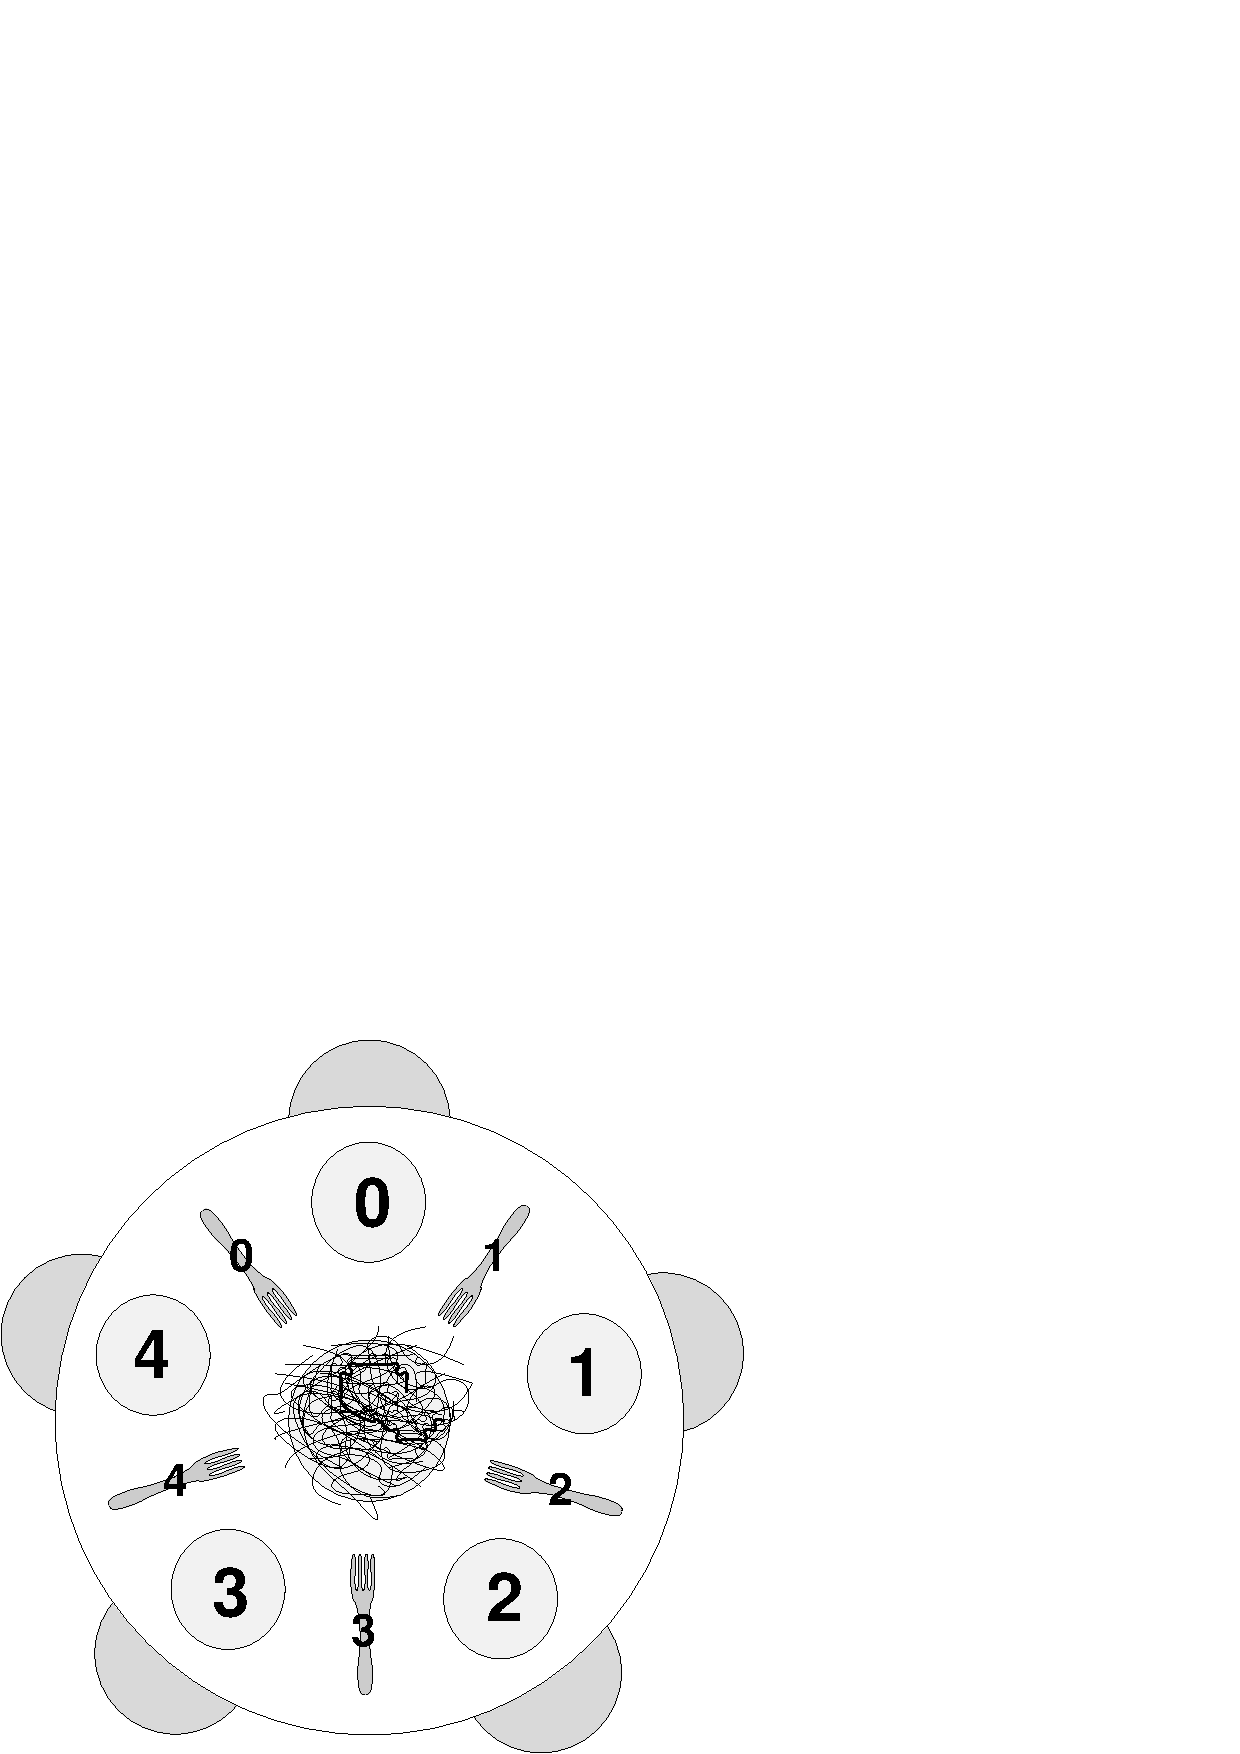
\includegraphics[height=2in]{table}}

Assuming that the philosophers know how to {\tt think} and {\tt eat},
our job is to write a version of {\tt get\_forks} and {\tt put\_forks}
that satisfies the following constraints:

\begin{itemize}

\item Only one philosopher can hold a fork at a time.

\item It must be impossible for a deadlock to occur.

\item It must be impossible for a philosopher to starve waiting
for a fork.

\item It must be possible for more than one philosopher
to eat at the same time.

\end{itemize}

Feltételezve, hogy a filozófusok tudják, hogyan kell gondolkodni
és enni, a mi feladatunk, hogy megírjuk {\tt megragadja\_a\_villákat} és
{\tt leteszi\_a\_villákat} egy olyan változatát, amelyek kielégítik a
következő korlátokat:

\begin{itemize}

\item Csak egy filozófus tarthat egyszerre egy villát.

\item Lehetetlennek kell lennie, hogy egy patthelyzet létrejöjjön.

\item Lehetetlennek kell lennie, hogy egy filozófus éhenhaljon villára várva.

\item Lehetségesnek kell lennie, hogy egyszerre több filozófus egyen.

\end{itemize}

The last requirement is one way of saying that the solution
should be efficient; that is, it should allow the maximum amount
of concurrency.

Az utolsó követelmény mondja ki azt, hogy a megoldásnak hatékonynak kell
lennie; vagyis az egyidejűségnek minél nagyobbnak kell lennie.

We make no assumption about how long {\tt eat} and {\tt think} take,
except that {\tt eat} has to terminate eventually.  Otherwise, the
third constraint is impossible---if a philosopher keeps one of the
forks forever, nothing can prevent the neighbors from starving.

To make it easy for philosophers to refer to their forks,
we can use the functions {\tt left} and {\tt right}:

Semmit nem feltételezünk {\tt gondolkozik} és {\tt eszik} futási idejéről,
csak azt, hogy az {\tt eszik}-nek valamikor be kell fejeződnie. Másképp
a harmadik korlát lehetetlen -- ha egy filozófus örökké tartja az
egyik villát, semmi sem képes megakadályozni a szomszédok éhhalálát.

Annak érdekében, hogy a filozófusok könnyen hivatkozhassanak a villákra,
a {\tt bal} és {\tt jobb} függvényeket használhatjuk:

\begin{lstlisting}[title={Which fork?}]{}
def left(i): return i
def right(i): return (i + 1) % 5
\end{lstlisting}

\begin{lstlisting}[title={Melyik villa?}]{}
def bal(i): return i
def jobb(i): return (i + 1) % 5
\end{lstlisting}

The {\tt \%} operator wraps around when it gets to 5, so
{\tt (4 + 1) \% 5 = 0}.

Since we have to enforce exclusive access to the forks,
it is natural to use a list of Semaphores, one for
each fork.  Initially, all the forks are available.

A {\tt \%} operátor körbefordul, amikor 5-re kerül, tehát {\tt (4 + 1) \% 5 = 0}.

Mivel kizárólagos hozzáférést kell biztosítanunk a villákhoz, ezért
természetes, hogy több szemafort használunk, minden villához egyet.
Kezdetben minden villa elérhető.

\begin{lstlisting}[title={Variables for dining philosophers}]{}
forks = [Semaphore(1) for i in range(5)]
\end{lstlisting}

\begin{lstlisting}[title={Változók a vacsorázó filozófusoknak}]{}
villák = [Szemafor(1) for i in range(5)]
\end{lstlisting}

This notation for initializing a list might be unfamiliar to
readers who don't use Python.  The {\tt range} function returns
a list with 5 elements; for each element of this list, Python
creates a Semaphore with initial value 1 and assembles the
result in a list named {\tt forks}.

Here is an initial attempt at {\tt get\_fork} and {\tt put\_fork}:

Ez a jelölés a lista inicializálására nem feltétlenül ismert az olvasók
körében, akik nem használják a Pythont. A {\tt range} függvény 5 elemet tartalmazó
listával tér vissza\footnote{Pontosabban egy iterátorral, de ez ebben a kódban lényegtelen.};
a lista minden egyes elemére a Python létrehoz egy
szemafort 1-es kezdeti értékkel, és összeállítja az eredményt egy {\tt villák}
nevű listában.

Itt van egy első próbálkozás a {\tt megragadja\_a\_villákat} és {\tt leteszi\_a\_villákat}-hoz:

\begin{lstlisting}[title={Dining philosophers non-solution}]{}
def get_forks(i):
    fork[right(i)].wait()
    fork[left(i)].wait()

def put_forks(i):
    fork[right(i)].signal()
    fork[left(i)].signal()
\end{lstlisting}

\begin{lstlisting}[title={Vacsorázó filozófusok nem-megoldás}]{}
def megragadja_a_villákat(i):
    villa[jobb(i)].vár()
    villa[bal(i)].vár()

def leteszi_a_villákat(i):
    villa[jobb(i)].jelez()
    villa[bal(i)].jelez()
\end{lstlisting}

It's clear that this solution satisfies the first constraint, but
we can be pretty sure it doesn't satisfy the other two, because
if it did, this wouldn't be an interesting problem and you would
be reading Chapter~\ref{next}.

Puzzle: what's wrong?

Nyilvánvaló, hogy ez a megoldás kielégíti az első megszorítást, de biztosak
lehetünk benne, hogy nem elégíti ki a másik kettőt, mert ha igen,
akkor ez nem lenne érdekes probléma, és akkor az \ref{next}. fejezetet olvasnánk.

Rejtvény: Mi a probléma?

\clearemptydoublepage
\subsection{Patthelyzet \#5}

The problem is that the table is round.  As a result, each philosopher
can pick up a fork and then wait forever for the other fork.  Deadlock!

Puzzle: write a solution to this problem that prevents deadlock.

Hint: one way to avoid deadlock is to think about the conditions
that make deadlock possible and then change one of those conditions.
In this case, the deadlock is fairly fragile---a very small change
breaks it.

A probléma az, hogy az asztal kerek. Ennek eredményeképpen minden
filozófus felvehet egy villát, majd örökké várja a másik villát.
Patthelyzet!

Rejtvény: Írj megoldást erre a problémára, amely megakadályozza
a patthelyzetet.

Tipp: a patthelyzet elkerülésének egyik módja az, hogy gondolkodjunk
el a körülményekről, amik lehetségessé teszik a holtpontot, majd
megváltoztatjuk az egyik ilyen feltételt. Ebben az esetben a patthelyzet
meglehetősen  törékeny -- nagyon kicsi változtatás is tönkreteszi.

\clearemptydoublepage
\subsection{Vacsorázó filozófusok tipp \#1}

If only four philosophers are allowed at the table at a time,
deadlock is impossible.

First, convince yourself that this claim is true, then write code that
limits the number of philosophers at the table.

Ha egyszerre csak négy filozófus ülhet az asztalnál, a patthelyzet lehetetlen.

Először győződjünk meg róla, hogy ez az állítás igaz, majd írjunk kódot,
amely korlátozza a filozófusok számát az asztalnál.

\clearemptydoublepage
\subsection{Vacsorázó filozófusok megoldás \#1}

If there are only four philosophers at the table, then in the
worst case each one picks up a fork.  Even then, there is a fork
left on the table, and that fork has two neighbors, each of
which is holding another fork.  Therefore, either of these
neighbors can pick up the remaining fork and eat.

Ha csak négy filozófus van az asztalnál, akkor a legrosszabb
esetben mindegyik felvesz egy villát. Még akkor is marad egy
villa az asztalon, és a villának két szomszédja van, amelyek
mindegyike egy másik villát tart. Ezért ezek a szomszédok
bármelyike felveheti a megmaradt villát és tud enni.

We can control the number of philosophers at the table with
a Multiplex named {\tt footman} that is initialized to 4.
Then the solution looks like this:


Az asztalnál ülő filozófusok számát tudjuk befolyásolni egy
multiplexel, amit inasnak hívnak, és kezdőállapota 4. Ezután
a megoldás így néz ki:

\begin{lstlisting}[title={Dining philosophers solution \#1}]{}
def get_forks(i):
    footman.wait()
    fork[right(i)].wait()
    fork[left(i)].wait()

def put_forks(i):
    fork[right(i)].signal()
    fork[left(i)].signal()
    footman.signal()
\end{lstlisting}

\begin{lstlisting}[title={Vacsorázó filozófusok megoldás \#1}]{}
def megragadja_a_villákat(i):
    inas.vár()
    villa[jobb(i)].vár()
    villa[bal(i)].vár()

def leteszi_a_villákat(i):
    villa[jobb(i)].jelez()
    villa[bal(i)].jelez()
    inas.jelez()
\end{lstlisting}

In addition to avoiding deadlock, this solution also guarantees that
no philosopher starves.
Imagine that you
are sitting at the table and both of your neighbors are eating.  You
are blocked waiting for your right fork.  Eventually your right
neighbor will put it down, because {\tt eat} can't run forever.  Since
you are the only thread waiting for that fork, you will necessarily
get it next.  By a similar argument, you cannot starve waiting for
your left fork.

A patthelyzet elkerülése mellett ez a megoldás azt is garantálja,
hogy egyetlen filozófus sem fog éhen halni. Képzeljük el, hogy
az asztalnál ülünk, és mindkét szomszédunk eszik. Mi blokkolva
várjuk a jobb villát. Végül a jobb szomszédunk leteszi, mert az
{\tt eszik} nem fut örökké. Mivel mi vagyunk az egyetlen szál, amelyik
várakozik erre a villára, szükségszerűen megkapjuk azt. Hasonlóan
érvelve a bal villára várva sem tudunk éhen halni.

Therefore, the time a philosopher can spend at the table is bounded.
That implies that the wait time to get into the room is also bounded,
as long as {\tt footman} has Property 4 (see Section ~\ref{props}).

Ezért az idő, amit a filozófus az asztalnál tud tölteni, korlátozott.
Ez azt jelenti, hogy a szobába bejutásra való várakozási idő is
szintén korlátozott, amíg az inas rendelkezik a 4. tulajdonsággal (lásd: \ref{props}-as rész).

This solution shows that
by controlling the number of philosophers, we can avoid deadlock.
Another way to avoid deadlock is to change the order in which the
philosophers pick up forks.  In the original non-solution, the
philosophers are ``righties''; that is, they pick up the right fork
first.  But what happens if Philosopher 0 is a leftie?

Ez a megoldás azt mutatja, hogy a filozófusok számának szabályozásával
elkerülhetjük a patthelyzetet. A patthelyzet elkerülésének másik módja az,
hogy megváltoztatjuk azt a sorrendet, amelyben a filozófusok felveszik
a villákat. Az eredeti nem-megoldásban a filozófusok jobbkezesek;
vagyis először a jobb villát veszik fel. De mi történik, ha a nulladik
filozófus balkezes?

Puzzle: prove that if there is at least one leftie and at least one
rightie, then deadlock is not possible.

Hint: deadlock can only occur when all 5 philosophers are holding
one fork and waiting, forever, for the other.  Otherwise, one of
them could get both forks, eat, and leave.

The proof works by contradiction.  First, assume that deadlock is
possible.  Then choose one of the supposedly deadlocked philosophers.
If she's a leftie, you can prove that the philosophers are all
lefties, which is a contradiction.  Similarly, if she's a rightie, you
can prove that they are all righties.  Either way you get a
contradiction; therefore, deadlock is not possible.

Rejtvény: Bizonyítsuk be, hogy ha van legalább egy jobbkezes, és
legalább egy balkezes, akkor nincs patthelyzet.

Tipp: a patthelyzet csak akkor alakulhat ki, ha mind az öt filozófus egy
villát tart és örökre várakozik a másikra. Ellenkező esetben egyikük
mindkét villát el tudná venni, enni, és elmenni.

Indirekt bizonyítást használunk. Először feltételezzük, hogy a patthelyzet
lehetséges. Ezután válasszunk egyet az állítólagosan patthelyzetben álló
filozófusok közül. Ha ő balkezes, akkor bebizonyíthatjuk, hogy a
filozófusok mindegyike balkezes, ami ellentmondás. Hasonlóképpen,
ha ő jobbkezes, akkor bizonyítani tudjuk, hogy mindannyian azok.
Mindkét esetben ellentmondást kapunk; ezért a patthelyzet nem lehetséges.

\clearemptydoublepage
\subsection{Vacsorázó filozófusok megoldás \#2}

In the asymmetric solution to the Dining philosophers problem,
there has to be at least one leftie and at least one rightie at
the table.  In that case, deadlock is impossible.  The previous
hint outlines the proof.  Here are the details.

Az éhes filozófusok problémájának aszimmetrikus megoldásakor
legalább egy balkezest és legalább egy jobbkezest kell elhelyezni
az asztalnál. Ebben az esetben a patthelyzet lehetetlen. Az előző tipp
vázolja a bizonyítást. Itt vannak a részletek.

Again, if deadlock is possible, it occurs when all 5 philosophers
are holding one fork and waiting for the other.  If we assume that
Philosopher $j$ is a leftie, then she must be holding her left
fork and waiting for her right.  Therefore her neighbor to the right,
Philosopher $k$, must be holding his left fork and waiting for
his right neighbor; in other words, Philosopher $k$ must be a leftie.
Repeating the same argument, we can prove that the philosophers
are all lefties, which contradicts the original claim that there
is at least one rightie.  Therefore deadlock is not possible.

Ismételten, ha lehetséges a patthelyzet, az akkor következik be, ha mind
az öt filozófus egy villát tart és vár a másikra. Ha feltételezzük,
hogy a $j$-dik filozófus balkezes, akkor meg kell tartania a bal villáját,
és a jobbra kell várnia. Ezért a jobboldali szomszédjának, a $k$-dik filozófusnak
a bal villáját kell tartania, és a jobb szomszédjára kell várnia;
más szóval, a $k$-dik filozófusnak balkezesnek kell lennie. Ismételve ezt az
érvet, be tudjuk bizonyítani, hogy a filozófusok mindegyike balkezes,
amely ellentmond az eredeti állításnak, hogy van legalább egy jobbkezes.
Ezért a patthelyzet nem lehetséges.

The same argument we used for the previous solution also proves
that starvation is impossible for this solution.

Ugyanaz az érvelés, amit az előző megoldásban használtunk azt is
bizonyítja, hogy az kiéheztetés lehetetlen ebben a megoldásban.

\clearemptydoublepage
\subsection{Tanenbaum megoldása}

There is nothing wrong with the previous solutions, but just for
completeness, let's look at some alternatives.  One of the best known
is the one that appears in Tanenbaum's popular operating systems
textbook \cite{tanenbaum}.
For each philosopher there is a state variable that
indicates whether the philosopher is thinking, eating, or waiting to
eat (``hungry'') and a semaphore that indicates whether the
philosopher can start eating.  Here are the variables:

Nincs semmi baj az előző megoldásokkal, de csak a teljesség kedvéért
nézzünk néhány alternatívát. Az egyik legismertebb az, amely
Tanenbaum népszerű operációs rendszerek könyvében \cite{tanenbaum} jelenik meg.
Minden filozófusnál van egy állapotváltozó, amely azt jelzi, hogy a
filozófus gondolkodik, eszik vagy várakozik az evésre („éhes”), és
egy szemafor, amely jelzi, hogy a filozófus elkezdhet-e enni.
Itt vannak a változók:

\begin{lstlisting}[title={Variables for Tanenbaum's solution}]{}
state = ['thinking'] * 5
sem = [Semaphore(0) for i in range(5)]
mutex = Semaphore(1)
\end{lstlisting}

\begin{lstlisting}[title={Változók Tanenbaum megoldásához}]{}
állapot = ['gondolkodik'] * 5
szem = [Szemafor(0) for i in range(5)]
kökiz = Szemafor(1)
\end{lstlisting}

The initial value of {\tt state} is a list of 5 copies of {\tt
'thinking'}.  {\tt sem} is a list of 5 semaphores with the initial
value 0.  Here is the code:

Az {\tt állapot} eredeti értéke a 'gondolkodik' 5 példányának a
listája. {\tt szem} 5 szemafor listája, mindegyik kezdeti értéke 0.
Itt van a kód:

\begin{lstlisting}[title={Tanenbaum's solution}]{}
def get_fork(i):
    mutex.wait()
    state[i] = 'hungry'
    test(i)
    mutex.signal()
    sem[i].wait()

def put_fork(i):
    mutex.wait()
    state[i] = 'thinking'
    test(right(i))
    test(left(i))
    mutex.signal()

def test(i):
    if state[i] == 'hungry' and
    state[left (i)]  != 'eating' and
    state[right (i)] != 'eating':
        state[i] = 'eating'
        sem[i].signal()
\end{lstlisting}

% NOTE: need to fix this; see email from David Furcy.

\begin{lstlisting}[title={Tanenbaum megoldása}]{}
def megragadja_a_villákat(i):
    kökiz.vár()
    állapot[i] = 'éhes'
    teszt(i)
    kökiz.jelez()
    szem[i].vár()

def leteszi_a_villákat(i):
    kökiz.vár()
    állapot[i] = 'gondolkodik'
    teszt(jobb(i))
    teszt(bal(i))
    kökiz.jelez()

def teszt(i):
    if állapot[i] == 'éhes' and
    állapot[bal (i)]  != 'eszik' and
    állapot[jobb (i)] != 'eszik':
        állapot[i] = 'eszik'
        szem[i].jelez()
\end{lstlisting}


The {\tt test} function checks whether the $i$th philosopher can
start eating, which he can if he is hungry and
neither of his neighbors are eating.  If so, the {\tt test} signals
semaphore $i$.

A {\tt teszt} függvény megnézi, hogy az $i$-dik filozófus elkezdhet-e enni,
amit megtehet akkor, ha éhes, és egyik szomszédja sem eszik. Ha ez
igaz, akkor a {\tt teszt} jelez az $i$-dik szemafornak.

There are two ways a philosopher gets to eat.  In the first case, the
philosopher executes {\tt get\_forks}, finds the forks available, and
proceeds immediately.  In the second case, one of the neighbors is
eating and the philosopher blocks on its own semaphore.  Eventually,
one of the neighbors will finish, at which point it executes {\tt
test} on both of its neighbors.  It is possible that both tests
will succeed, in which case the neighbors can run concurrently.
The order of the two tests doesn't matter.

A filozófus kétféle módon tud enni. Az első esetben a filozófus
végrehajtja a {\tt megragadja\_a\_villákat} függvényt, meglátja, hogy mindkét villa elérhető,
és azonnal elindul. A második esetben az egyik szomszéd eszik, és a filozófus
saját szemaforát blokkolja. Végül az egyik szomszéd végez, ekkor mindkét
szomszédra végrehajtja {\tt teszt}-et. Lehetséges, hogy mindkét teszt sikeres lesz, ebben
az esetben a szomszédok egyidejűleg futhatnak. A két teszt sorrendje nem számít.

In order to access {\tt state} or invoke {\tt test}, a thread
has to hold {\tt mutex}.  Thus, the operation of checking and
updating the array is atomic.  Since a philosopher can only proceed
when we know both forks are available, exclusive access to the forks
is guaranteed.

Annak érdekében, hogy elérje az {\tt állapot}-ot vagy meghívja a {\tt teszt}-et,
a szálnak tartania kell a {\tt kökiz}-t. Így a tömb ellenőrzése és frissítése atomi.
Mivel a filozófus csak akkor tud tovább futni, ha tudjuk, hogy mindkét villa elérhető,
garantált a kizárólagos hozzáférés a villákhoz.

No deadlock is possible, because the only semaphore that is accessed
by more than one philosopher is {\tt mutex}, and no thread executes
{\tt wait} while holding {\tt mutex}.

Nem lehet patthelyzet, mert az egyetlen szemafor, amelyet egynél több filozófus
ér el az a {\tt kökiz}, és nincs szál ami végrehajtana egy {\tt vár()}-t a {\tt kökiz}
tartása közben.

But again, starvation is tricky.

Puzzle: Either convince yourself that Tanenbaum's solution prevents
starvation or find a repeating pattern that allows a thread to starve
while other threads make progress.

Azonban ne feledjük, hogy a kiéheztethetőség trükkösebb.

Rejtvény: Vagy győződjünk meg arról, hogy a Tanenbaum megoldás megakadályozza
az kiéheztetést, vagy keressünk egy olyan ismétlődő mintát, amely lehetővé teszi
egy szálnak, hogy éhenhaljon, míg más szálak haladnak.

\clearemptydoublepage
\subsection{Éhes Tanenbaumok}

Unfortunately, this solution is not starvation-free.  Gingras
demonstrated that there are repeating patterns that allow a
thread to wait forever while other threads come and go
\cite{gingras90dining}.

Sajnos ez a megoldás nem kiéheztetésmentes. Gingras bizonyította, hogy vannak
olyan ismétlődő minták, amelyek lehetővé teszik, hogy egy szál állandóan
várjon, míg más szálak jönnek és mennek \cite{gingras90dining}.

Imagine that we are trying to starve Philosopher 0.  Initially,
2 and 4 are at the table and 1 and 3 are hungry.  Imagine that 2 gets up and
1 sit downs; then 4 gets up and 3 sits down.
Now we are in the mirror image of the starting position.

Képzeljük el, hogy megpróbáljuk kiéheztetni a 0. filozófust.
Kezdetben 2. és 4. az asztalnál van, az 1. és 3. pedig éhes.
Képzeljük el, hogy 2. felkel és 1. ül le; majd 4. felkel és 3. leül.
Most a kezdő pozíció tükörképében vagyunk.

If 3 gets up and 4 sits
down, and then 1 gets up and 2 sits down, we are back
where we started.  We could repeat the cycle indefinitely and
Philosopher 0 would starve.

Ha 3. felkel és 4. ül le, majd 1. felkel és 2. ül le, visszaértünk oda,
ahol elkezdtük. A ciklust akárhányszor ismételhetjük, és a 0. filozófus éhenhal.

So, Tanenbaum's solution doesn't satisfy all the requirements.

Tehát Tanenbaum megoldása nem felel meg az összes követelménynek.


\clearemptydoublepage
\section{A civakodó háziasszonyok problémája}

A civakodó háziasszonyok problémája eredetileg a dohányosok
cigaretta problémája néven szerepel a szakirodalomban (cigarette smokers problem),
de mivel a magyar fordítás szerkesztője semmilyen formában
nem kívánja propagálni e káros szenvedélyt, ezért átfogalmaztuk.
A civakodó háziasszonyok ötlete Fehér Andrástól származik.

The cigarette smokers problem was originally presented by
Suhas Patil \cite{patil}, who claimed that it cannot be solved with
semaphores.  That claim comes with some qualifications, but in
any case the problem is interesting and challenging.

A dohányosok cigaretta problémáját eredetileg Suhas Patil vetette fel\cite{patil},
aki azt állította, hogy nem lehet megoldani
szemaforokkal. Ez az állitás néhány kitételt igényel, de mindenesetre
a probléma érdekes és kihívást jelent.


Four threads are involved: an agent and three smokers.  The smokers
loop forever, first waiting for ingredients, then making and smoking
cigarettes.  The ingredients are tobacco, paper, and matches.

We assume that the agent has an infinite supply of all three
ingredients, and each smoker has an infinite supply of one of
the ingredients; that is, one smoker has matches, another has
paper, and the third has tobacco.

The agent repeatedly chooses two different ingredients at random
and makes them available to the smokers.  Depending on which
ingredients are chosen, the smoker with the complementary ingredient
should pick up both resources and proceed.

Három háziasszony kertipartyt szervezett, de mielőtt belekezdtek
volna a melegszendvicsek legyártásába, összevesztek valamin, és most
nem hajlandók együttműködni. Sajnos az egyikük hozta a sajtot, a másikuk a
sonkát, a harmadikuk pedig a kenyeret, így most egyikük sem tud
melegszendvicset készíteni, csak az asztal körül ülnek, és csúnyán néznek egymásra.
Időnként egy éhes vendég betéved a konyhába, és ki tudja honnan
a melegszendvics három alkotóeleméből kettőt letesz az asztalra.
Ekkor az a háziasszony, akinél a harmadik hozzávaló található, felveszi
a másik kettőt, és készít egy adag melegszendvicset, majd bánatosan
visszaül az asztalhoz.

Feltételezzük, hogy a háziasszonyok sosem fogynak ki a saját
hozzávalójukból, és a vendégek is folyton kerítenek véletlenszerűen
egy-egy adagnyit kettő hozzávalóból.

For example, if the agent puts out tobacco and paper, the
smoker with the matches should pick up both ingredients, make
a cigarette, and then signal the agent.


Például, ha egy vendég sajtot és kenyeret tesz le az asztalra,
a háziasszony, aki a sonkát hozta, felveheti mindkét
hozzávalót, készíthet egy melegszendvicset, majd jelezheti
a vendégseregnek, hogy ismét lerakhatnak két összetevőt.
(Feltételezzük, hogy sütés közben nem tartózkodhatnak illetékteleneknek
a konyhában.)

To explain the premise, the agent represents an operating system that
allocates resources, and the smokers represent applications that need
resources.  The problem is to make sure that if resources are
available that would allow one more applications to proceed,
those applications should be woken up.  Conversely, we want to avoid
waking an application if it cannot proceed.

Ennek a helyzetnek a lényege az, hogy a vendég reprezentálja az operációs rendszert,
ami kiosztja az erőforrásokat, és a háziasszonyok szimbolizálják az alkalmazásokat
amiknek erőforrásokra van szükségük. A probléma annak biztosítása,
hogy ha rendelkezésre állnak az erőforrások ahhoz, hogy még egy alkalmazás
folytassa a futást, akkor azt az alkalmazást fel kell kelteni.
Fordítva, meg akarjuk akadályozni azoknak
az alkalmazásoknak a felkeltését, amik nem tudnak tovább futni.


Based on this premise, there are three versions of this problem
that often appear in textbooks:

Ezekkel az előfeltételekkel háromfajta változatban szokott ez a probléma
feltűnni a tankönyvekben.


\begin{description}

\item[The impossible version:] Patil's version imposes restrictions on
the solution.  First, you are not allowed to modify the agent code.
If the agent represents an operating system, it makes sense to assume
that you don't want to modify it every time a new application comes
along.  The second restriction is that you can't use conditional
statements or an array of semaphores.  With these constraints, the
problem cannot be solved, but as Parnas points out, the second
restriction is pretty artificial \cite{Parnas}.  With constraints like
these, a lot of problems become unsolvable.

\item[The interesting version:] This version keeps the first
restriction---you can't change the agent code---but it drops the others.

\item[The trivial version:] In some textbooks, the problem specifies
that the agent should signal the smoker that should go next, according
to the ingredients that are available.  This version of the problem
is uninteresting because it makes the whole premise, the ingredients
and the cigarettes, irrelevant.  Also, as a practical matter, it is
probably not a good idea to require the agent to know about the other
threads and what they are waiting for.  Finally, this version of
the problem is just too easy.


\item[A lehetetlen változat:] Patil verziója további korlátozásokat
tesz a megoldásra. Először is a vendég kódját nem szaban megváltoztatni.
Ha a vendég az operációs rendszert jelképezi, akkor ésszerű a feltevés hogy
nem akarjuk mindig megváltoztatni, ahányszor egy új applikáció elindul.
A második korlátozás az, hogy nem használhatunk feltételes utasítást vagy
egy szemafor tömböt. Ezekkel a feltételekkel a problémát nem lehet megoldani,
de amint Parnas rámutatott \cite{Parnas}, a második kitétel eléggé életszerűtlen.
Ilyen feltételekkel nagyon sok probléma megoldhatatlan lesz.

\item[Az érdekes változat:] Ez a verzió megtartja az első kitételt, hogy a vendég
kódját nem szaban megváltoztatni, de a többit eldobja.

\item[A triviális változat:] Néhány könyvben a feladat specifikálja, hogy a vendégnek
jeleznie kell a háziasszonynak, aki a következő lesz a szabad hozzávalók szerint.
Ez a változat a problémát érdektelené teszi, mert az egész előfeltételben foglalt
hozzávalókat és a melegszendvicset irrelevánssá teszi. Gyakorlatilag pedig nem jó ötlet megkövetelni a vendégtől,
hogy tudjon a többiekről és arról, hogy mire várnak. Végül pedig, ez a változat túl könnyű.

\end{description}

Naturally, we will focus on the interesting version.  To complete
the statement of the problem, we need to specify the agent code.
The agent uses the following semaphores:

Természetesen mi az érdekes verzióra fogunk koncentrálni. Hogy 
teljessé tegyük a probléma meghatározását, definiálni kell a vendég kódját.
A vendég a következő szemaforokat használja:

\begin{lstlisting}[title={Agent semaphores}]{}
agentSem = Semaphore(1)
tobacco = Semaphore(0)
paper = Semaphore(0)
match = Semaphore(0)
\end{lstlisting}

\begin{lstlisting}[title={A vendég szemaforai}]{}
vendégSzem = Szemafor(1)
sajt = Szemafor(0)
sonka = Szemafor(0)
kenyér = Szemafor(0)
\end{lstlisting}

The agent is actually made up of three concurrent
threads, Agent A, Agent B and Agent C.  Each waits on
{\tt agentSem}; each time {\tt agentSem} is signaled,
one of the Agents wakes up and provides ingredients by
signaling two semaphores.

A vendég valójában három konkurens szálból áll: SaSo vendég,
SoKe vendég és KeSa vendég. Mindegyikük {\tt vendégSzem}-re vár. Minden egyes
alkalommal, amikor {\tt vendégSzem} jelez, egy a vendégek közül felkel,
és elérhetővé tesz hozzávalókat azzal, hogy jelez
két szemafornak.

\begin{lstlisting}[title={Agent A code}]{}
agentSem.wait()
tobacco.signal()
paper.signal()
\end{lstlisting}

\begin{lstlisting}[title={Agent B code}]{}
agentSem.wait()
paper.signal()
match.signal()
\end{lstlisting}

\begin{lstlisting}[title={Agent C code}]{}
agentSem.wait()
tobacco.signal()
match.signal()
\end{lstlisting}

\begin{lstlisting}[title={SaSo vendég kód}]{}
vendégSzem.vár()
sajt.jelez()
sonka.jelez()
\end{lstlisting}

\begin{lstlisting}[title={SoKe vendég kód}]{}
vendégSzem.vár()
sonka.jelez()
kenyér.jelez()
\end{lstlisting}

\begin{lstlisting}[title={KeSa vendég kód}]{}
vendégSzem.vár()
kenyér.jelez()
sajt.jelez()
\end{lstlisting}

This problem is hard because the natural solution does not
work.  It is tempting to write something like:

Ez a probléma nehéz, mert a természetes megoldás nem működik.
Csábító írni valami ilyesmit:

\begin{lstlisting}[title={Smoker with matches}]{}
tobacco.wait()
paper.wait()
agentSem.signal()
\end{lstlisting}

\begin{lstlisting}[title={Smoker with tobacco}]{}
paper.wait()
match.wait()
agentSem.signal()
\end{lstlisting}

\begin{lstlisting}[title={Smoker with paper}]{}
tobacco.wait()
match.wait()
agentSem.signal()
\end{lstlisting}

\begin{lstlisting}[title={Kenyeres háziasszony}]{}
sajt.vár()
sonka.vár()
süt()
vendégSzem.jelez()
\end{lstlisting}

\begin{lstlisting}[title={Sajtos háziasszony}]{}
sonka.vár()
kenyér.vár()
süt()
vendégSzem.jelez()
\end{lstlisting}

\begin{lstlisting}[title={Sonkás háziasszony}]{}
kenyér.vár()
sajt.vár()
süt()
vendégSzem.jelez()
\end{lstlisting}

What's wrong with this solution?

Rejtvény: Mi a probléma ezzel a megoldással?

\clearemptydoublepage
\subsection{Patthelyzet \#6}

The problem with the previous solution is the possibility
of deadlock.  Imagine that the agent puts out tobacco and
paper.  Since the smoker with matches is waiting on {\tt tobacco},
it might be unblocked.  But the smoker with tobacco is
waiting on {\tt paper}, so it is possible (even likely) that
it will also be unblocked.  Then the first thread will block
on {\tt paper} and the second will block on {\tt match}.
Deadlock!

A probléma az előző megoldással a patthelyzet lehetősége.
Képzeljük el azt, hogy a vendég kirakja a sajtot és a sonkát.
Mivel a „kenyeres háziasszony” vár a {\tt sajt}-on, lehet, hogy felébred.
De a „sajtos háziasszony” a {\tt sonká}-n vár, így megvan a lehetősége annak
(sőt, igen valószínű), hogy ő is felébred. Ekkor az első szál a {\tt sonká}-n,
a második a {\tt kenyér}-en fog blokkolódni. Patthelyzet!

\clearemptydoublepage
\subsection{Civakodó háziasszonyok problémája tipp}

The solution proposed by Parnas uses three helper threads
called ``pushers'' that respond to the signals from the agent,
keep track of the available ingredients, and signal the
appropriate smoker.

The additional variables and semaphores are

A Parnas javasolta megoldás három segítő szálat használ, amiket
„pusher”-nek hívunk, amik válaszolnak a vendég jelzésére, nyomon követik
a szabad hozzávalókat, és jeleznek a megfelelő háziasszonynak.

A megfelelő változók és szemaforok:

\begin{lstlisting}[title={Smokers problem hint}]{}
isTobacco = isPaper = isMatch = False
tobaccoSem = Semaphore(0)
paperSem = Semaphore(0)
matchSem = Semaphore(0)
\end{lstlisting}

\begin{lstlisting}[title={Civakodó háziasszonyok tipp}]{}
vanSajt = vanSonka = vanKenyér = False
sajtSzem = Szemafor(0)
sonkaSzem = Szemafor(0)
kenyérSzem = Szemafor(0)
kökiz = Szemafor(1)
\end{lstlisting}

The boolean variables indicate whether or not an ingredient
is on the table.  The pushers use {\tt tobaccoSem} to signal
the smoker with tobacco, and the other semaphores likewise.

A bool változók jelzik, milyen erőforrás van az asztalon.
A pusherek a {\tt sajtSzem}-et használják, hogy jelezzenek a „sajtos háziasszonynak”,
a {\tt sonkaSzem}-et, hogy a „sonkás háziasszonynak” és a {\tt kenyérSzem}-et, hogy a „kenyeres háziasszonynak”.
{\tt kökiz} védi a bool változókat.

\clearemptydoublepage
\subsection{Civakodó háziasszonyok problémája megoldás}

Here is the code for one of the pushers:

Itt van a kód az egyik tolóhoz:

\begin{lstlisting}[title={Pusher A}]{}
tobacco.wait()
mutex.wait()
    if isPaper:
        isPaper = False
        matchSem.signal()
    elif isMatch:
        isMatch = False
        paperSem.signal()
    else: 
        isTobacco = True
mutex.signal()
\end{lstlisting}

\begin{lstlisting}[title={Toló A}]{}
sonka.vár()
kökiz.vár()
    if vanSajt:
        vanSajt = False
        kenyérSzem.jelez()
    elif vanKenyér:
        vanKenyér = False
        sajtSzem.jelez()
    else: 
        vanSonka = True
kökiz.jelez()
\end{lstlisting}


This pusher wakes up any time there is tobacco on the
table.  If it finds {\tt isPaper} true, it knows that
Pusher B has already run, so it can signal the smoker
with matches.  Similarly, if it finds a match on the
table, it can signal the smoker with paper.

But if Pusher A runs first, then it will find both
{\tt isPaper} and {\tt isMatch} false.  It cannot signal
any of the smokers, so it sets {\tt isTobacco}.

The other pushers are similar.  Since the pushers do all
the real work, the smoker code is trivial:

Ez a pusher akkor aktiválódik ha az asztalon van sonka.
Ha azt látja, hogy {\tt vanSajt} igaz , akkor tudja hogy a Pusher B
már lefutott, szóval akkor jelez a megfelelő háziasszonynak.

De ha a Pusher A fut először, akkor a {\tt vanSajt} és a {\tt vanKenyér}
is hamis, ilyenkor nem tud egyik háziasszonynak sem jelezni ezért
átállítja a {\tt vanSonká}-t.

A többi Pusher is hasonlókép működik. Mivel a Pusherek végzik
az igazi munkát, a dohányosok kódja triviális:

\begin{lstlisting}[title={Smoker with tobacco}]{}
tobaccoSem.wait()
makeCigarette()
agentSem.signal()
smoke()
\end{lstlisting}

\begin{lstlisting}[title={Sajtos háziasszony}]{}
sajtSzem.vár()
süt()
vendégszemSzem.jelez()
haragszikABarátnőire()
\end{lstlisting}

Parnas presents a similar solution that assembles the
boolean variables, bitwise, into an integer, and then
uses the integer as an index into an array of semaphores.
That way he can avoid using conditionals (one of the
artificial constraints).  The resulting code is a bit
more concise, but its function is not as obvious.

Parnas bemutat egy hasonló megoldást, ami összeállítja a
bool változókat bitenként egy integerré, és utána az integert
használja mint index egy szemafortömbhöz. Így
el tudta kerülni a feltételek használatát. Az eredményként kapott
kód egy kicsit tömörebb, de a működése nem annyira egyértelmű.

\subsection{Általánosított civakodó háziasszonyok problémája}

Parnas suggested that the smokers problem becomes more
difficult if we modify the agent, eliminating the requirement
that the agent wait after putting out ingredients.  In this
case, there might be multiple instances of an ingredient on
the table.

Puzzle: modify the previous solution to deal with this
variation.

Parnas azt mondta, hogy a civakodó háziasszonyok problémája nehezebb lesz,
ha módosítjuk az vendéget, eltörölve azt a feltételt hogy
a vendégnek várnia kell, miután kirakta a hozzávalókat.
Ebben az esetben ugyanabból a hozzávalóból egyszerre több darab
is lehet az asztalon.

Rejtvény: módosítsd az előző megoldást hogy működőképes legyen
ezzel a variációval.

\clearemptydoublepage
\subsection{Általánosított civakodó háziasszonyok problémája tipp}

If the agents don't wait for the smokers, ingredients might
accumulate on the table.  Instead of using boolean values to
keep track of ingredients, we need integers to count them.

Ha a vendégek nem várnak a melegszendvicsekre, a hozzávalók felhalmozódhatnak
az asztalon. Ahelyett, hogy bool értékeket használnánk, egész
számokra lesz szükségünk a nyomon követésükhöz.

\begin{lstlisting}[title={Generalized Smokers problem hint}]{}
numTobacco = numPaper = numMatch = 0
\end{lstlisting}

\begin{lstlisting}[title={Általánosított civakodó háziasszonyok problémája tipp}]{}
sajtSzám = sonkaSzám = kenyérSzám = 0
\end{lstlisting}

\clearemptydoublepage
\subsection{Általánosított civakodó háziasszonyok problémája megoldás}
\label{smoker}

Here is the modified code for Pusher A:

Itt a módosított kód a Pusher A-hoz:

\begin{lstlisting}[title={Pusher A}]{}
tobacco.wait()
mutex.wait()
    if numPaper:
        numPaper -= 1
        matchSem.signal()
    elif numMatch:
        numMatch -= 1
        paperSem.signal()
    else: 
        numTobacco += 1
mutex.signal()
\end{lstlisting}

\begin{lstlisting}[title={Pusher A}]{}
sonka.vár()
kökiz.vár()
    if sonkaSzám > 0:
        sonkaSzám -= 1
        kenyérSzem.jelez()
    elif kenyérSzám > 0:
        kenyérSzám -= 1
        sonkaSzem.jelez()
    else: 
        sonkaSzám += 1
kökiz.jelez()
\end{lstlisting}

One way to visualize this problem is to imagine that when an
Agent runs, it creates two pushers, gives each of them one ingredient,
and puts them in a room with all the other pushers.  Because of the
mutex, the pushers file into a room where there are
three sleeping smokers and a table.  One at a time, each pusher enters
the room and checks the ingredients on the table.  If he can
assemble a complete set of ingredients, he takes them off the table
and wakes the corresponding smoker.  If not, he leaves his ingredient
on the table and leaves without waking anyone.

Egy lehetőség az is hogyha vizualizáljuk a problémát és elképzeljük,
hogy amikor az ügynök fut, akkor létrehoz két darab pushert, mindegyiknek
ad egy-egy darab hozzávalót, és utána berakja őket egy szobába az
összes pusherrel együtt. A mutex miatt, a pusher iktat a szobában,
ahol a három dohányzó és az asztal található. Egyesével mindegyik
pusher bemegy a szobába és megnézik, hogy milyen hozzávalók vannak
az asztalon. Ha képes összerakni a három hozzávalót akkor elveszi
az asztalról majd felébreszti a megfelelő dohányost. Ha nem akkor
csak leteszi a hozzávalót az asztalra és kimegy a szóbából anélkül,
hogy bárkit felkeltene.

Úgy is elképzelhetjük a megoldást, hogy amikor a vendég fut, létrehoz
két tolót, mindegyiknek ad egy hozzávalót, és beküldi őket egy szobába a többi
tolóhoz. A kökiz miatt a tolók egyesével mennek át a konyhába,
és megnézik, mi van az asztal közepén. Ha ebből össze tudnak állítani
egy melegszendvicset, a szükséges két dolgot odatolják valamelyik háziasszonyhoz,
aki ebből süthet. (Ha éppen az előző melegszendvicset süti, a két új hozzávaló akkor
is csak rá vár az asztalon.)

This is an example of a pattern we will see several times, which
I call a {\bf scoreboard}.  The variables {\tt numPaper}, {\tt numTobacco}
and {\tt numMatch} keep track of the state of the system.  As each
thread files through the mutex, it checks the state as if looking
at the scoreboard, and reacts accordingly.

Ez egy példa egy olyan sémára amit nagyon sok alkalommal fogunk látni,
és én {\bf műszerfalnak} hívom. A változók, {\tt dohánySzám}, {\tt papírszám} és {\tt gyufaSzám}
folyamatosan követik a rendszer állapotát. 
Miközben minden egyes szál átverekszi magát a kökizen,
ellenőrzi a helyzetet, mintha egy műszerfalat nézne, és annak megfelelően reagál.

\clearemptydoublepage
\chapter{Kevésbé klasszikus szinkronizációs problémák}
\label{next}


\section{Az étkező vademberek problémája}

This problem is from Andrews's 
{\em Concurrent Programming} \cite{andrews}.

\begin {quotation}
A tribe of savages eats communal dinners from a large pot that can
hold M servings of stewed missionary\footnote{This problem is based on
a cartoonish representation of the history of Western missionaries
among hunter-gatherer societies.  Some humor is intended by the
allusion to the Dining Philosophers problem, but the representation of
``savages'' here isn't intended to be any more realistic than the
previous representation of philosophers.  If you are interested in
hunter-gatherer societies, I recommend Jared Diamond's {\em Guns,
Germs and Steel}, Napoleon Chagnon's {\em The Yanomamo}, and Redmond
O'Hanlon's {\em In Trouble Again}, but not Tierney's {\em Darkness in
El Dorado}, which I believe is unreliable.}.  When a savage wants to
eat, he helps himself from the pot, unless it is empty.  If the pot is
empty, the savage wakes up the cook and then waits until the cook has
refilled the pot.
\end{quotation}

Any number of savage threads run the following code:

Ez a feladat Andrews {\em Concurrent Programming} \cite{andrews}
című könyvéből való.

\begin {quotation}
Egy vademberekből álló törzs közös vacsorát tart egy olyan kondérból,
amiben $M$ adag pirított misszionárius fér el. Ha egy vadember enni akar,
akkor kiszolgálja magát a kondérból, kivéve, ha az üres. Ha a kondér üres,
akkor a vadember felkelti a szakácsot és megvárja, amíg a szakács
megtölti azt.
\end{quotation}

Tetszőleges számú vadember szál a következő kódot futtatja:

\begin{lstlisting}[title={Unsynchronized savage code}]{}
while True:
    getServingFromPot()
    eat()
\end{lstlisting}

\begin{lstlisting}[title={Szinkronizálatlan vadember kód}]{}
while True:
    kiszolgáljaMagátAKondérból()
    eszik()
\end{lstlisting}

And one cook thread runs this code:

És egy szakács szál ezt a kódot futtatja:

\begin{lstlisting}[title={Szinkronizálatlan szakács kód}]{}
while True:
    megtöltiAKondért(M)
\end{lstlisting}

The synchronization constraints are:

\begin{itemize}

\item Savages cannot invoke {\tt getServingFromPot} if the
pot is empty.

\item The cook can invoke {\tt putServingsInPot} only if
the pot is empty.

\end{itemize}

Puzzle: Add code for the savages and the cook that
satisfies the synchronization constraints.

A szinkronizációs megszorítások az alábbiak:

\begin{itemize}

\item A vademberek nem hívhatják meg a {\tt kiszolgáljaMagátAKondérból}-t, ha a kondér üres.
\item A szakács csak akkor hívhatja meg a {\tt megtöltiAKondért} függvényt, ha a kondér üres.

\end{itemize}

Rejtvény: Adj olyan kódot a vademberekhez és a szakácshoz,
amik megfelelnek a szinkronizációs megszorításoknak.

\clearemptydoublepage
\subsection{Étkező vademberek tipp}

It is tempting to use a semaphore to keep track of the number of
servings, as in the producer-consumer problem.  But in order to signal
the cook when the pot is empty, a thread would have to know before
decrementing the semaphore whether it would have to wait, and we just
can't do that.

An alternative is to use a scoreboard to
keep track of the number of servings.  If a savage finds
the counter at zero, he wakes the cook and waits for a signal
that the pot is full.  Here are the variables I used:

Csábító, hogy egy szemafort használjunk az adagok számontartására,
mint a termelő-fogyasztó feladatban. De ahhoz hogy
a szakács  jelt kapjon, amikor a fazék üres, egy szálnak tudnia kellene
a szemafor csökkentése előtt, hogy várnia kellene-e és ezt
nem tudjuk megcsinálni.

Egy alternatíva az, hogy egy műszerfalat használunk az
adagok számontartására. Ha egy vadember a számlálót nullán
találja, akkor felkelti a szakácsot és vár arra, hogy
megteljen a fazék. Itt vannak a változók, amiket használtam:
	
\begin{lstlisting}[title={Dining Savages hint}]{}
servings = 0
mutex = Semaphore(1)
emptyPot = Semaphore(0)
fullPot = Semaphore(0)
\end{lstlisting}

\begin{lstlisting}[title={Étkező vademberek tipp}]{}
adagok = 0
kökiz = Szemafor(1)
üresFazék = Szemafor(0)
teliFazék = Szemafor(0)
\end{lstlisting}

Not surprisingly, {\tt emptyPot} indicates that the pot is empty and
{\tt fullPot} indicates that the pot is full.

Nem meglepő módon az {\tt üresFazék} azt jelzi, hogy
a fazék üres és a {\tt teliFazék} pedig, hogy a fazék tele van.

\clearemptydoublepage
\subsection{Étkező vademberek megoldás}

My solution is a combination of the scoreboard pattern
with a rendezvous.
Here is the code for the cook:

Az én megoldásom az műszerfal minta és egy randevú kombinációja.

Itt van a kód a szakácshoz:

\begin{lstlisting}[title={Dining Savages solution (cook)}]{}
while True:
    emptyPot.wait()
    putServingsInPot(M)
    fullPot.signal()
\end{lstlisting}

\begin{lstlisting}[title={Étkező vademberek megoldás (szakács)}]{}
while True:
    üresFazék.vár()
    megtöltiAKondért(M)
    teliFazék.jelez()
\end{lstlisting}

The code for the savages is only a little more complicated.
As each savage passes through the mutex, he checks the pot.
If it is empty, he signals the cook and waits.  Otherwise,
he decrements {\tt servings} and gets a serving from the pot.

A kód a vademberekhez csak egy kicsit komplikáltabb.
Ahogy az egyes vademberek áthaladnak a kökizen, leellenőrzik
a fazekat. Ha az üres, akkor jeleznek a szakácsnak és várnak. Amúgy
csökkentik eggyel az {\tt adagok}-at és kivesznek egyet a fazékból.

\begin{lstlisting}[title={Dining Savages solution (savage)}]{}
while True:
    mutex.wait()
        if servings == 0:
            emptyPot.signal()
            fullPot.wait()
            servings = M
        servings -= 1
	getServingFromPot()
    mutex.signal()

    eat()
\end{lstlisting}

\begin{lstlisting}[title={Étkező vademberek megoldás (vadember)}]{}
while True:
    kökiz.vár()
        if adagok == 0:
            üresFazék.jelez()
            teliFazék.vár()
            adagok = M
        adagok -= 1
	kiszolgáljaMagátAKondérból()
    kökiz.jelez()

    eszik()
\end{lstlisting}

It might seem odd that the savage, rather than the cook, sets
{\tt servings = M}.  That's not really necessary; when the cook
runs {\tt putServingsInPot}, we know that the savage that holds
the mutex is waiting on {\tt fullPot}.  So the cook could
access {\tt servings} safely.  But in this case, I decided to
let the savage do it so that it is clear from looking at the
code that all accesses to {\tt servings} are inside the mutex.

Lehet, hogy szokatlannak tűnik, hogy a szakács helyett a vadember
állítja be az {\tt adagok = M}-et. Ez nem feltétlen szükséges; amikor
a szakács {\tt megtöltiAKondért}-ot futtatja, tudjuk, hogy a vadember,
akinél a kökiz van, a {\tt teliFazék}-ra vár. Szóval a szakács biztonságosan
hozzáférhetne az {\tt adagok}-hoz. De ebben az esetben úgy gondoltam,
hogy hagyom, hogy a vadember csinálja azért, hogy a kódra nézve
nyilvánvaló legyen, hogy az {\tt adagok}-hoz való minden hozzáférés
a kökizen belül történik.

This solution is deadlock-free.  The only opportunity for
deadlock comes when the savage that holds {\tt mutex} waits
for {\tt fullPot}.  While he is waiting, other savages are
queued on {\tt mutex}.  But eventually the cook will run and
signal {\tt fullPot}, which allows the waiting savage
to resume and release the mutex.

Ez a megoldás patthelyzetmentes. Az egyetlen
lehetőség patthelyzetre akkor lehetne, amikor a
vadembernél van a {\tt kökiz} és vár a {\tt teliFazék}-ra. Amíg vár, más
vademberek sorban állnak a {\tt kökiz}-ért. De végül a szakács le fog
futni és jelzi a {\tt teliFazék}-ot, ami lehetővé teszi a várakozó
vadembernek, hogy továbblépjen és elengedje a kökizt.

Does this solution assume that the pot is thread-safe, or does it
guarantee that {\tt putServingsInPot} and {\tt getServingFromPot}
are executed exclusively?

Kérdés: 
Feltételezi-e ez a megoldás, hogy a fazék szál-biztos vagy
garantálja-e azt, hogy a {\tt kiszolgáljaMagátAKondérból} és a {\tt megtöltiAKondért}
egymást kizárva vannak végrehajtva?

\clearemptydoublepage
\section{A fodrászüzlet probléma}

The original barbershop problem was proposed by
Dijkstra.  A variation of it appears in 
Silberschatz and Galvin's {\em Operating Systems Concepts}
\cite{silberschatz}.

Az eredeti fodrászüzlet problémát Dijkstra vetette fel.
Egy variációja feltűnik Silberschatz és Galvin
{\em Operating System Concepts} című könyvében \cite{silberschatz}.

\begin{quotation}
A barbershop consists of a waiting room with $n$ chairs, and the
barber room containing the barber chair.  If there are no customers to
be served, the barber goes to sleep.  If a customer enters the
barbershop and all chairs are occupied, then the customer leaves the
shop.  If the barber is busy, but chairs are available, then the
customer sits in one of the free chairs.  If the barber is asleep, the
customer wakes up the barber.  Write a program to coordinate the
barber and the customers.
\end{quotation}

\begin{quotation}
A fodrászatnak van egy váróterme $n$ db. székkel, illetőleg
egy fodrász szobája egy darab fodrászszékkel. Amennyiben
nincs kiszolgálásra váró ügyfél, a fodrász aludni tér.
Ha belép az üzletbe egy ügyfél és minden szék foglalt,
akkor az ügyfél elhagyja a fodrászatot. Amennyiben a fodrász dolgozik,
de vannak szabad székek, akkor az újonnan betért ügyfél helyet foglal
az egyik szabad széken. Ha a fodrász alszik, az ügyfél felébreszti őt.
Írj egy programot a fodrász és az ügyfelek koordinálására!
\end{quotation}

To make the problem a little more concrete, I added the
following information:

Hogy egy kissé kézzelfoghatóbbá tegyük a problémát, a következő
információkkal egészítjük ki:

\begin{itemize}

\item Customer threads should invoke a function named {\tt getHairCut}.

\item If a customer thread arrives when the shop is full, 
it can invoke {\tt balk}, which does not return.

\item The barber thread should invoke {\tt cutHair}.

\item When the barber invokes {\tt cutHair} there should
be exactly one thread invoking {\tt getHairCut} concurrently.

\end{itemize}

\begin{itemize}

\item Az ügyfél szálak meghívhatnak egy {\tt megnyírnak} függvényt.
\item Ha egy ügyfél szál akkor érkezik meg, mikor a fodrászat tele van,
meg tudja hívni az {\tt elmegy} függvényt, amely nem fog visszatérni.
\item A fodrász szál képes meghívni a {\tt hajvágás} függvényt.
\item Amikor a fodrász meghívja a {\tt hajvágás} függvényt, konkurensen képes
meghívni pontosan egy szál a {\tt megnyírnak} függvényt.
\end{itemize}

Write a solution that guarantees these constraints.

Rejtvény:
Írj egy megoldást, mely garantálja ezeket a feltételeket!


\clearemptydoublepage
\subsection{Fodrászüzlet tipp}

\lstinputlisting[title=Barbershop hint]{../code/barber.py.0}

\begin{lstlisting}[title={Fodrászüzlet tipp}]{}
n = 4
ügyfelek = 0
kökiz = Szemafor(1)
ügyfél = Szemafor(0)
fodrász = Szemafor(0)
ügyfélKész = Szemafor(0)
fodrászKész = Szemafor(0)
\end{lstlisting}

{\tt n} is the total number of customers that can be in the shop:
three in the waiting room and one in the chair.

{\tt customers} counts the number of customers in the shop;
it is protected by {\tt mutex}.

The barber waits on {\tt customer} until a customer enters the
shop, then the customer waits on {\tt barber} until the barber
signals him to take a seat.

After the haircut, the customer signals {\tt customerDone} and
waits on {\tt barberDone}.

{\tt n} az összes ügyfél száma, akik a fodrászatban tartózkodhatnak:
három a váróteremben egy pedig a fodrászszékben.

{\tt ügyfelek} számolja az ügyfeleket a fodrászatban, ez {\tt kökiz} által védve van.

A fodrász addig vár {\tt vendég}-re, amíg egy ügyfél be nem lép a fodrászatba,
azután pedig az ügyfél vár a {\tt fodrász}-ra, amíg a fodrász jelet nem ad, hogy foglaljon helyet.

A hajvágás után az ügyfél jelzi a {\tt ügyfélKész}-t és vár a {\tt fodrászKész}-re. 

\clearemptydoublepage
\subsection{Fodrászüzlet megoldás}

This solution combines a scoreboard and two rendezvouses\footnote{The
  plural of rendezvous is rare, and not all dictionaries agree about
  what it is.  Another possibility is that the plural is also spelled
  ``rendezvous,'' but the final ``s'' is pronounced.}.  Here is the
code for customers:

Ez a megoldás egy műszerfalat és két randevút kombinál. Az ügyfelekhez tartozó kód:

\lstinputlisting[title=Barbershop solution (customer)]{../code/barber.py.1}

\begin{lstlisting}[title={Fodrászüzlet megoldás (ügyfél)}]{}
kökiz.vár()
    if ügyfelek == n:
        kökiz.jelez()
        elmegy()
    vendégek += 1
mutex.jelez()

ügyfél.jelez()
fodrász.vár()

megnyírnak()

ügyfélKész.jelez()
fodrászKész.vár()

kökiz.vár()
    ügyfelek -= 1
kökiz.jelez()
\end{lstlisting}

If there are $n$ customers in the shop any customers that
arrive immediately invoke {\tt balk}.
Otherwise each customer signals {\tt customer} and waits on
{\tt barber}.

Amennyiben $n$ db. ügyfél tartózkodik az üzletben, akármelyik újonnan
érkező ügyfél azonnal meghívja az {\tt elmegy} függvényt. Egyébként mindegyik
ügyfél jelzi {\tt ügyfél}-t és vár {\tt fodrász}-ra.


Here is the code for barbers:

A fodrászhoz tartozó kód:

\lstinputlisting[title=Barbershop solution (barber)]{../code/barber.py.2}

\begin{lstlisting}[title={Fodrászüzlet megoldás (ügyfél)}]{}
ügyfél.vár()
fodrász.jelez()

hajvágás()

ügyfélKész.vár()
fodrászKész.jelez()

\end{lstlisting}

Each time a customer signals,
the barber wakes, signals {\tt barber}, and gives one
hair cut.  If another customer arrives while the barber
is busy, then on the next iteration the barber will pass
the {\tt customer} semaphore without sleeping.

Minden alkalommal, amikor az ügyfél jelez, a fodrász felkel, jelzi
{\tt fodrász}-t és ad egy hajvágást. Ha akkor érkezik egy ügyfél, amikor
a fodrász elfoglalt, akkor a következő iterációkor a fodrász az {\tt ügyfél}
szemaforon megállás nélkül fog áthaladni.

The names for {\tt customer} and {\tt barber} are based on
the naming convention for a rendezvous, so {\tt customer.wait()}
means ``wait for a customer,'' not ``customers wait here.''

Az {\tt ügyfél} és a {\tt fodrász} változónevek a randevú névkonvencióján alapszanak, tehát
az {\tt ügyfél.vár()} azt jelenti, „várj az ügyfélre”, nem pedig azt, hogy „ügyfelek várjatok itt”.

The second rendezvous, using {\tt customerDone} and {\tt barberDone},
ensures that the hair cut is done before the barber loops around to
let the next customer into the critical section.

A második randevú {\tt ügyfélKész}-szel és {\tt fodrászKész}-szel
biztosítja, hogy a hajvágás kész lesz, mielőtt a fodrász körbehalad,
hogy új ügyfelet engedjen a kritikus szakaszba.

This solution is in \verb"sync_code/barber.py" (see~\ref{sync.py}).


\clearemptydoublepage
\section{EBEK fodrászüzlet}

In the previous solution there is no guarantee that customers are
served in the order they arrive.  Up to {\tt n} customers can pass
the turnstile, signal
{\tt customer} and wait on {\tt barber}.  When the barber signal
{\tt barber}, any of the customers might proceed.

Az előző megoldásban nincs rá garancia, hogy az ügyfeleket
érkezési sorrendben szolgálják ki. Akár {\tt n} ügyfél is átmehet a
forgóajtón, jelezheti {\tt ügyfél}-t, és várhat {\tt fodrász}-ra.
Amikor a fodrász jelzi {\tt fodrász}-t, bármelyikük továbbhaladhat.

Modify this solution so that customers are served in the order they
pass the turnstile.

Rejtvény: Módosítsd ezt a megoldást úgy, hogy az ügyfelek abban a sorrendben
legyenek kiszolgálva, ahogy áthaladtak a forgóajtón.

Hint: you can refer to the current thread as {\tt self}, so if you
write {\tt self.sem = Semaphore(0)}, each thread gets its own
semaphore.

Tipp: az aktuális szálra hivatkozhatunk, mint {\tt self}, tehát
ha azt írjuk, {\tt self.szem = Szemafor(0)}, akkor mindegyik
szálnak lesz egy saját szemaforja.

\clearemptydoublepage
\subsection{EBEK fodrászüzlet tipp}

My solution uses a list of semaphores named {\tt queue}.

A megoldásom egy szemaforlistát használ, aminek a neve {\tt sor}.

\lstinputlisting[title=FIFO barbershop hint]{../code/barber2.py.0}

\begin{lstlisting}[title={EBEK fodrászüzlet tipp}]{}
n = 4
ügyfelek = 0
kökiz = Szemafor(1)
ügyfél = Szemafor(0)
ügyfélKész = Szemafor(0)
fodrászKész = Szemafor(0)
sor = []
\end{lstlisting}

As each thread passes the turnstile, it creates a thread and puts it
in the queue.

Ahogy egy szál áthalad a forgóajtón, létrehoz egy szemafort,
és beteszi a sorba.

Instead of waiting on {\tt barber}, each thread waits on its own
semaphore.  When the barber wakes up, he removes a thread from the queue and
signals it.

Ahelyett, hogy {\tt fodrász}-on várnának, mindegyik szál a saját
szemaforán vár. Amikor a fodrász felébred, kiveszi a szemafort a sorból,
és jelez rajta.


\clearemptydoublepage
\subsection{EBEK fodrászüzlet megoldás}

Here is the modified code for customers:

Íme a módosított kód az ügyfeleknek:

\lstinputlisting[title=FIFO barbershop solution (customer)]
{../code/barber2.py.1}

\begin{lstlisting}[title={EBEK fodrászüzlet megoldás (ügyfél)}]{}
self.szem =  = Szemafor(0)
kökiz.vár()
    if ügyfelek == n:
        kökiz.jelez()
        elmegy()
    ügyfelek += 1
    sor.append(self.szem)
kökiz.jelez()

ügyfél.jelez()
self.szem.vár()

megnyírnak()

ügyfélKész.jelez()
fodrászKész.vár()

kökiz.vár()
    ügyfelek -= 1
kökiz.jelez()
\end{lstlisting}

And the code for barbers:

És a fodrásznak:

\lstinputlisting[title=FIFO barbershop solution (barber)]
{../code/barber2.py.2}

\begin{lstlisting}[title={EBEK fodrászüzlet megoldás (fodrász)}]{}
ügyfél.vár()
kökiz.vár()
    szem = sor.pop(0)
kökiz.jelez()

szem.jelez()

hajvágás()

ügyfélKész.vár()
fodrászKész.jelez()
\end{lstlisting}

Notice that the barber has to get {\tt mutex} to access the
queue.

Figyeljük meg, hogy a fodrásznak birtokolnia kell {\tt kökiz}-t,
hogy hozzáférjen a sorhoz.

This solution is in \verb"sync_code/barber2.py" (see~\ref{sync.py}).


\clearemptydoublepage
\section{Hilzer fodrászata probléma}

William Stallings \cite{stallings} presents a more complicated version
of the barbershop problem, which he attributes to Ralph Hilzer at the
California State University at Chico.

William Stallings \cite{stallings} publikálta egy bonyolultabb verzióját a fodrászüzlet problémának,
amit Ralph Hilzer-nek tulajdonít a Kalifornia Állam Egyetemen Chicoban.

\begin{quotation}
Our barbershop has three chairs, three barbers, and a waiting
area that can accommodate four customers on a sofa and that has
standing room for additional customers.  Fire codes limit the
total number of customers in the shop to 20.

A customer will not enter the shop if it is filled to capacity with
other customers.  Once inside, the customer takes a seat on the sofa
or stands if the sofa is filled.  When a barber is free, the customer
that has been on the sofa the longest is served and, if there are any
standing customers, the one that has been in the shop the longest
takes a seat on the sofa.  When a customer's haircut is finished, any
barber can accept payment, but because there is only one cash
register, payment is accepted for one customer at a time.  The barbers
divide their time among cutting hair, accepting payment, and sleeping
in their chair waiting for a customer.
\end{quotation}

\begin{quotation}
A fodrászatunknak van három széke, három fodrásza, és egy váró, ahol
négy ügyfél tud leülni egy kanapéra és további ügyfelek várakozhatnak állva.
A tűzvédelmi előírások miatt a fodrászatban egyszerre legfeljebb 20 ügyfél tartózkodhat.

Egy ügyfél nem lép be az üzletbe, ha az már tele van ügyfelekkel.
Bent az ügyfél helyet foglal a kanapén, vagy áll, ha a kanapén nincs hely.
Ha egy fodrász szabad, azt az ügyfelet aki a legrégebb óta ült a kanapén
szolgálják ki és, ha van állva várakozó ügyfél , akkor aki a legrégebb óta
várakozik állva, az helyet foglal a kanapén. Ha egy ügyfél hajvágása kész,
akkor bármelyik fodrásznak lehet fizetni, de mivel csak egy kassza van,
ezért egy időben csak egy ügyfél fizethet. A fodrászok felosztják az
idejüket a hajvágás,  fizetés és székükben alvás között
amíg várnak az ügyfelekre.
\end{quotation}


In other words, the following synchronization constraints apply:

\begin{itemize}

\item Customers invoke the following functions in order:
{\tt enterShop}, {\tt sitOnSofa},
{\tt getHairCut}, {\tt pay}.

\item Barbers invoke {\tt cutHair} and {\tt acceptPayment}.

\item Customers cannot invoke {\tt enterShop} if the shop
is at capacity.

\item If the sofa is full, an arriving customer cannot invoke 
{\tt sitOnSofa}.

\item When a customer invokes {\tt getHairCut} there should be
a corresponding barber executing {\tt cutHair} concurrently,
and vice versa.

\item It should be possible for up to three customers to execute
{\tt getHairCut} concurrently, and up to three barbers to execute
{\tt cutHair} concurrently.

\item The customer has to {\tt pay} before the barber can
{\tt acceptPayment}.

\item The barber must {\tt acceptPayment} before the customer can
exit.

\end{itemize}

Puzzle: Write code that enforces the synchronization
constraints for Hilzer's barbershop.

Másszóval, a következők a szinkronizációs megszorítások:

\begin{itemize}

\item Az ügyfelek a következő függvényeket hívják meg sorban:
{\tt belépAFodrászatba}, {\tt kanapénÜl}, {\tt megnyírnak}, {\tt fizet}.

\item A fodrászok a {\tt hajvágás} és a {\tt kaszírozás} függvényeket hívják meg.

\item Az ügyfelek nem hivhatják meg a {\tt belépAFodrászatba} függvényt, ha a fodrászat tele van.

\item Ha a kanapé tele van, az érkező ügyfél nem hivhatja meg a {\tt kanapénÜl} függvényt.

\item Ha egy ügyfél meghívja a {\tt megnyírnak} függvényt, akkor kell lennie egy
megfelelő fodrásznak, aki egyidejűleg végrehajtja a {\tt hajvágás} függvényt,
és fordítva.

\item Lehetővé kell tenni, hogy akár három ügyfél is végrehajthassa
a {\tt megnyírnak} függvényt egyidőben, és akár 3 fodrász végrehajthassa a {\tt hajvágás}
függvényt egyidőben.

\item Az ügyfélnek még azelőtt kell fizetni, mielőtt a fodrász végrehajtja
a {\tt kaszírozás} függvényt.

\item A fodrásznak az előtt kell végrehajtania a {\tt kaszírozás} függvényt,
mielőtt az ügyfél távozna.

\end{itemize}

Rejtvény: Írj kódot, ami végrehajtja a szinkronizációs korlátokat Hilzer fodrászathoz.

\subsection{Hilzer fodrászata tipp}

Here are the variables I used in my solution:

Ezeket a változókat használtam a megoldásomban:

\lstinputlisting[title=Hilzer's barbershop hint]
{../code/barber3.py.0}

\begin{lstlisting}[title={Hilzer fodrászata tipp}]{}
n = 20
ügyfelek = 0
kökiz = Szemafor(1)
kanapé = Szemafor(4)
ügyfél1 = Szemafor(0)
ügyfél2 = Szemafor(0)
fodrász = Szemafor(0)
fizetés = Szemafor(0)
nyugta = Szemafor(0)
sor1 = []
kökiz2 = Szemafor(1)
sor2 = []
\end{lstlisting}

{\tt mutex} protects {\tt customers}, which keeps track of the
number of customers in the shop, and {\tt queue1} which is a list
of semaphores for threads waiting for a seat on the sofa.

{\tt mutex2} protects {\tt queue2}, which is a list
of semaphores for threads waiting for a chair.

{\tt sofa} is a multiplex that enforces the maximum number of customers
on the sofa.

{\tt customer1} signals that there is a customer in {\tt queue1}, and
{\tt customer2} signals that there is a customer in {\tt queue2}.

{\tt payment} signals that a customer has paid, and {\tt receipt}
sigmals that a barber has accepted payment.

{\tt kökiz} védi az {\tt ügyfelek}-et, ami az ügyfelek számát jelöli a fodrászatban,
és {\tt sor1}-et ami egy lista a kanapén helyre várakozó szálak szemaforjainak.

{\tt kökiz2} védi  {\tt sor2}-t, ami egy lista a székre várakozó szálak szemaforjainak.

{\tt kanapé} egy multiplex, ami az ügyfelek maximális számát korlátozza a kanapén.

{\tt ügyfél1} jelöli, hogy van-e ügyfél {\tt sor1}-ben, és {\tt ügyfél2} jelöli,
hogy van-e ügyfél {\tt sor2}-ben.

{\tt fizetés} jelöli, hogy az ügyfél fizetett, és {\tt nyugta} jelöli, hogy a fodrász
elfogadta a fizetést.

\clearemptydoublepage
\subsection{Hilzer fodrászata megoldás}

This solution is considerably more complex than I expected.  I
am not if Hilzer had something simpler in mind, but here is the
best I could do.

Ez a megoldás jóval bonyolultabb, mint vártam. Nem tudom,
hogy Hilzernek volt-e egyszerűbb megoldása, de ez a legjobb amit tudok.

\lstinputlisting[title=Hilzer's barbershop solution (customer)]
{../code/barber3.py.1}

\begin{lstlisting}[title={Hilzer fodrászata megoldás (ügyfél)}]{}
self.szem1 = Szemafor(0)
self.szem2 = Szemafor(0)

kökiz.vár()
    if ügyfelek == n:
        kökiz.jelez()
        elmegy()
    ügyfelek += 1
    sor1.append(self.szem1)
kökiz.jelez()

belépAFodrászatba()
ügyfél1.jelez()
self.szem1.vár()

kanapé.vár()
    kanapénÜl()
    self.szem1.jelez()
    kökiz.vár()
        sor2.append(self.szem2)
    kökiz.jelez()
    ügyfél2.jelez()
    self.szem2.vár()
kanapé.jelez()

megnyírnak()

fizet()
fizetés.jelez()
nyugta.vár()

kökiz.vár()
    ügyfelek -= 1
kökiz.jelez()
\end{lstlisting}

The first paragraph is the same as in the previous solution.  When
a customer arrives, it checks the counter and either balks or adds
itself to the queue.  Then it signals a barber.

When the customer gets out of queue, it enters the multiplex,
sits on the couch and adds itself to the second queue.

When it gets out of {\em that} queue, it gets a haircut, pays,
and then exits.

Az első bekezdés, ugyan az, mint az előző megoldásban. Amikor egy ügyfél
megérkezik, ellenőrzi a számlálót és vagy akadályba ütközik és elmegy, vagy beáll
a sorba. Majd jelez egy fodrásznak.

Amikor az ügyfél kikerül a sorból, akkor belép a multiplexbe,
leül a kanapéra és hozzáadja magát a második sorhoz.

Amikor kikerül {\em abból} a sorból, akkor kap egy hajvágást, fizet, majd távozik.
    
\lstinputlisting[title=Hilzer's barbershop solution (barber)]
{../code/barber3.py.2}

\begin{lstlisting}[title={Hilzer fodrászata megoldás (fodrász)}]{}
ügyfél1.vár()
kökiz.vár()
    szem = sor1.pop(0)
    szem.jelez()
    szem.vár()
kökiz.jelez()
szem.jelez()

ügyfél2.vár()
kökiz.vár()
    szem = sor2.pop(0)
kökiz.jelez()
szem.jelez()

fodrász.jelez()
hajvágás()

fizetés.vár()
kaszíroz()
nyugta.jelez()

\end{lstlisting}

Each barber waits for a customer to enter, signals the customer's
semaphore to get it out of queue, then waits for it to claim a seat
on the sofa.  This enforces the FIFO requirement.

Minden fodrász vár egy ügyfélre, hogy belépjen, jelzi az ügyfél szemaforjának,
hogy kerüljön ki a sorból, majd vár, hogy helyet foglaljon az ügyfél a
fodrász székben. Ez az EBEK követelményt hajtja végre.

The barber waits for the customer to join the second queue and then
signals it, allowing the customer to claim a chair.

A fodrász vár az ügyfélre, hogy csatlakozzon a második sorhoz és jelezzen,
majd az ügyfél engedélyt kap, hogy beüljön egy székbe.

Each barber admits one customer to the chair, so there can by up
to three concurrent haircuts.  Because there is only one cash
register, the customer has to get {\tt mutex}.  The customer
and barber rendezvous at the cash register, then both exit.

Minden fodrász egy ügyfelet fogad a székében, tehát akár három konkurens
hajvágás is lehet egyszerre. Mivel csak egy kassza van, az ügyfélnek
{\tt kökiz}-t kell birtokolnia. Az ügyfél és a fodrász randevúznak a kasszánál,
majd mindketten kilépnek.

This solution satisfies the synchonization constraints, but it leaves
the sofa underutilized.  Because there are only three barbers, there
can never be more than three customers on the sofa, so the multiplex
is unnecessary.

Ez a megoldás kielégíti a szinkronizációs megszorításokat, de a kanapét
kihasználatlanul hagyja. Mivel csak három fodrász van, soha nem lehet több
három ügyfélnél a kanapén, tehát a multiplex szükségtelen.

This solution is in \verb"sync_code/barber3.py" (see~\ref{sync.py}).

Ez a megoldás a \verb"sync_code/barber3.py" fájlban található (lásd~\ref{sync.py}).

The only way I can think of to solve this problem is to create a third
kind of thread, which I can an usher.  The ushers manage {\tt queue1}
and the barbers manage {\tt queue2}.  If there are 4 ushers and 3 barbers,
the sofa can be fully utilized.

This solution is in \verb"sync_code/barber4.py" (see~\ref{sync.py}).

Az egyetlen megoldás erre a problémára, amit el tudok képzelni, hogy létrehozunk egy
harmadik típusú szálat, amit jegyszedőnek hívhatunk. A jegyszedők kezelik {\tt sor1}-et
és a fodrászok kezelik {\tt sor2}-t. Ha van 4 jegyszedő és 3 fodrász, akkor
a kanapét teljesen ki lehet használni.

Ennek a megoldása a \verb"sync_code/barber4.py" (lásd~\ref{sync.py}).
   
\clearemptydoublepage
\section{A Mikulás probléma}

This problem is from William Stallings's
{\em Operating Systems} \cite{stallings},
but he attributes it to John Trono of St. Michael's College in
Vermont.

Ez a probléma William Stallings {\em Operating Systems} \cite{stallings}
című könyvéből származik, de ő a vermonti St. Michael's College-ban dolgozó
John Trono-nak tulajdonította.

\begin{quotation}
Santa Claus sleeps in his shop at the North Pole and can only be
awakened by either (1) all nine reindeer being back from their
vacation in the South Pacific, or (2) some of the elves having
difficulty making toys; to allow Santa to get some sleep, the elves
can only wake him when three of them have problems.  When three elves
are having their problems solved, any other elves wishing to visit
Santa must wait for those elves to return.  If Santa wakes up to find
three elves waiting at his shop's door, along with the last reindeer
having come back from the tropics, Santa has decided that the elves can
wait until after Christmas, because it is more important to get his
sleigh ready.  (It is assumed that the reindeer do not want to leave
the tropics, and therefore they stay there until the last possible
moment.)  The last reindeer to arrive must get Santa while the others
wait in a warming hut before being harnessed to the sleigh.
\end{quotation}

\begin{quotation}
A Mikulás az Északi-sarkon alszik az üzletében és csak akkor ébred fel,
ha (1) mind a kilenc rénszarvas visszatért a Dél-Csendes-óceáni vakációjáról,
vagy (2) néhány manónak problémái adódnak a játékok készítésével. Hogy a Mikulás
aludhasson, a manók csak akkor ébreszthetik fel, ha hármuknak is problémája van.
Ha három manó problémája megoldódott, akkor bármelyik másik manónak, aki meg
akarja látogatni a Mikulást, várnia kell, míg az a három manó vissza nem ér.
Ha a Mikulás felkel, és azt találja, hogy három manó vár rá az üzlete ajtajában,
és az utolsó rénszarvas is visszatért a trópusokról, a Mikulás döntése alapján a
manóknak várniuk kell Karácsony utánig, mert sokkal fontosabb, hogy készen
álljon a szánja. (Feltételezzük, hogy a rénszarvasok nem akarják elhagyni a
trópusokat, és ezért ott maradnak az utolsó pillanatig.) Az utolsó rénszarvas,
aki megérkezik, annak kell a Mikuláshoz mennie, míg a többiek egy kunyhóban
melegednek, mielőtt felkantározzák őket a szánhoz.
\end{quotation}


Here are some addition specifications:

\begin {itemize}

\item After the ninth reindeer arrives, Santa must invoke 
{\tt prepareSleigh}, and then all nine reindeer must
invoke {\tt getHitched}.

\item After the third elf arrives, Santa must invoke {\tt helpElves}.
Concurrently, all three elves should invoke {\tt getHelp}.

\item All three elves must invoke {\tt getHelp} before any additional
elves enter (increment the elf counter).

\end {itemize}

Santa should run in a loop so he can help many sets of elves.
We can assume that there are exactly 9 reindeer, but there may
be any number of elves.  

Íme néhány kiegészítő feltétel:

\begin {itemize}

\item Miután a kilencedik rénszarvas megérkezett, a Mikulásnak meg kell
hívnia a {\tt felkészítiASzánt}-ot, és utána mind a kilenc rénszarvasnak meg
kell hívnia a {\tt befogjákASzánba}-t.

\item Miután a harmadik manó is megérkezett, a Mikulásnak meg kell
hívnia {\tt segítAManóknak}-ot. Ezzel párhuzamosan mind a három
manónak {\tt segítségetKap}-ot kell meghívnia.

\item Mind a három manónak meg kell hívni a {\tt segítségetKap}-ot, mielőtt további
manók lépnek be (növekszik a törpe számláló).

\end {itemize}
A Mikulás egy végtelen ciklusban fusson, hogy minél több manónak tudjon segíteni.
Feltételezhetjük, hogy pontosan kilenc rénszarvas van, de lehet bármennyi manó.

\clearemptydoublepage
\subsection{Mikulás probléma tipp}

\begin{lstlisting}[title={Santa problem hint}]{}
elves = 0
reindeer = 0
santaSem = Semaphore(0)
reindeerSem = Semaphore(0)
elfTex = Semaphore(1)
mutex = Semaphore(1)
\end{lstlisting}

\begin{lstlisting}[title={Mikulás probléma tipp}]{}
manók = 0
rénszarvasok = 0
mikulásSzem = Szemafor(0)
rénszarvasSzem = Szemafor(0)
manóKiz = Szemafor(1)
kökiz = Szemafor(1)
\end{lstlisting}

{\tt elves} and {\tt reindeer} are counters, both protected
by {\tt mutex}.  Elves and reindeer get {\tt mutex} to modify the
counters; Santa gets it to check them.

Santa waits on {\tt santaSem} until either an elf or a reindeer
signals him.

The reindeer wait on {\tt reindeerSem} until Santa signals them to
enter the paddock and get hitched.

The elves use {\tt elfTex} to prevent additional elves from
entering while three elves are being helped.

{\tt manók} és {\tt rénszarvasok} számlálók,
mindkettőt {\tt kökiz} védi.  A manóknak és a rénszarvasoknak birtokolniuk kell a
{\tt kökiz}-t hogy módosíthassák a számlálókat; a Mikulásnak pedig, hogy kiolvassa azokat.

A Mikulás vár a {\tt mikulásSzem}-re, amig vagy egy manó, vagy egy rénszarvas nem jelez neki.

A rénszarvasok várnak a {\tt rénszarvasSzem}-re amíg a Mikulás nem jelez, hogy beléphetnek
a pajtába és befoghatja őket a szánhoz.

A manók a {\tt manóKiz}-t használják, hogy megakadályozzák a további
manók bejutását, miközben három manónak segít a Mikulás.

\clearemptydoublepage
\subsection{Mikulás probléma megoldás}

Santa's code is pretty straightforward.  Remember that it
runs in a loop.

A Mikulás kódja nagyon egyszerű. Ne feledjük, hogy egy végtelen ciklusban fut.


\begin{lstlisting}[title={Santa problem solution (Santa)}]{}
santaSem.wait()
mutex.wait()
    if reindeer >= 9:
        prepareSleigh()
        reindeerSem.signal(9)
        reindeer -= 9
    else if elves == 3:
        helpElves()
mutex.signal()
\end{lstlisting}

\begin{lstlisting}[title={Mikulás probléma megoldás (Mikulás)}]{}
mikulásSzem.vár()
kökiz.vár()
    if rénszarvasok >= 9:
        felkészítiASzánt()
        rénszarvasSzem.jelez(9)
        rénszarvasok -= 9
    else if manók == 3:
        segítAManóknak()
kökiz.jelez()
\end{lstlisting}

When Santa wakes up, he checks which of the two conditions
holds and either deals with the reindeer or the waiting elves.
If there are nine reindeer waiting,
Santa invokes {\tt prepareSleigh}, then signals {\tt reindeerSem}
nine times, allowing the reindeer to invoke {\tt getHitched}.
If there are elves waiting, Santa just
invokes {\tt helpElves}.  There is no need for the elves to wait
for Santa; once they signal {\tt santaSem}, they can
invoke {\tt getHelp} immediately.

Santa doesn't have to decrement
the {\tt elves} counter because the elves do it on their way
out.

Amikor a Mikulás felébred, megvizsgálja, hogy a két feltétel közül melyik teljesül,
és vagy foglalkozik a rénszarvasokkal vagy a várakozó manókkal. Ha kilenc
rénszarvas vár, a Mikulás meghívja a {\tt felkészítiASzánt}-ot, majd jelzi a
{\tt rénszarvasSzem}-et kilenc alkalommal, lehetővé téve a rénszarvasoknak
hogy meghívják a {\tt befogjákASzánba}-t. Ha vannak várakozó manók, a Mikulás csak
meghívja {\tt segítAManóknak}-ot. Nincs szükség arra, hogy a manók várjanak a
Mikulásra; miután jelezték a {\tt mikulásSzem}-et, azonnal meghívhatják
a {\tt segítségetKap}-ot.

A Mikulásnak nem kell csökkentenie a {\tt manók} számlálót, mert a manók ezt megteszik távozáskor.

Here is the code for reindeer:

Itt a kód a rénszarvasokhoz:


\begin{lstlisting}[title={Santa problem solution (reindeer)}]{}
mutex.wait()
    reindeer += 1
    if reindeer == 9:
        santaSem.signal()
mutex.signal()

reindeerSem.wait()
getHitched()
\end{lstlisting}

\begin{lstlisting}[title={Mikulás probléma megoldás (rénszarvasok)}]{}
kökiz.vár()
    rénszarvasok += 1
    if rénszarvasok == 9:
        mikulásSzem.jelez()
kökiz.jelez()

rénszarvasSzem.vár()
befogjákASzánba()
\end{lstlisting}


The ninth reindeer signals Santa and then joins the other
reindeer waiting on {\tt reindeerSem}.  When Santa signals, the
reindeer all execute {\tt getHitched}.

A kilencedik rénszarvas jelez a Mikulásnak és utána csatlakozik a többi
rénszarvashoz várva a {\tt rénszarvasSzem}-et. A Mikulás jelzésekor mindegyik
rénszarvas végrehajtja a {\tt befogjákASzánba} utasítást.

The elf code is similar, except that when the third elf arrives
it has to bar subsequent arrivals until the first three have
executed {\tt getHelp}.

A manó kód hasonló, kivéve, ha a harmadik manó megérkezik, akkor meg
kell akadályozni a további érkezéseket amíg az első három végre nem hajtja
a {\tt segítségetKap} utasítást.

\newpage
\begin{lstlisting}[title={Santa problem solution (elves)}]{}
elfTex.wait()
mutex.wait()
    elves += 1
    if elves == 3:
        santaSem.signal()
    else
        elfTex.signal()
mutex.signal()

getHelp()

mutex.wait()
    elves -= 1
    if elves == 0:
       elfTex.signal()
mutex.signal()
\end{lstlisting}

\begin{lstlisting}[title={Mikulás probléma megoldás (manók)}]{}
manóKiz.vár()
kökiz.vár()
    manók += 1
    if manók == 3:
        mikulásSzem.jelez()
    else
        manóKiz.jelez()
kökiz.jelez()

segítségetKap()

kökiz.vár()
    manók -= 1
    if manók == 0:
       manóKiz.jelez()
kökiz.jelez()
\end{lstlisting}

The first two elves release {\tt elfTex} at the same time they release
the {\tt mutex}, but the last elf holds {\tt elfTex}, barring other
elves from entering until all three elves have invoked {\tt getHelp}.

The last elf to leave releases {\tt elfTex}, allowing the
next batch of elves to enter.

Az első két manó elengedi a {\tt manóKiz}-t, pontosan akkor amikor elengedik
a {\tt kökiz}-t, de az utolsó manó tartja a {\tt manóKiz}-t, kizárva más
manókat a belépésből, amíg mind a három manó meg nem hívja {\tt segítségetKap}-ot.

Az utolsó manó elengedi {\tt manóKiz}-t, ezzel megengedve a következő
csapat manónak a belépést.

\newpage
\section{H$_2$O építés}
\label{water}

This problem has been a staple of the Operating Systems class
at U.C. Berkeley for at least a decade.  It seems to be based on
an exercise in Andrews's {\em Concurrent Programming} \cite{andrews}.

There are two kinds of threads, oxygen and hydrogen.  In order
to assemble these threads into water molecules, we have to
create a barrier that makes each thread wait until a
complete molecule is ready to proceed.

As each thread passes the barrier, it should invoke
{\tt bond}.  You must guarantee that all the threads
from one molecule invoke {\tt bond} before any of the threads
from the next molecule do.

Ez a probléma legalább egy évtizedig az egyik legfontosabb kérdés
volt a U.C. Berkeley Operációs Rendszerek óráján. Ránézésre Andrews
Párhuzamos Programozásának \cite{andrews} egyik feladatán alapul.

Kétfajta szálunk van, az egyik az oxigén, a másik a hidrogén.
Annak érdekében, hogy a szálakból egy vízmolekulát hozhassunk létre,
egy akadályt állítunk, mely várakozásra kényszeríti addig a szálakat,
míg egy teljes molekula készen nem ál a létrehozásra.

Amikor a szálak áthaladnak az akadályon, meg kell hívniuk a {\tt köt}
függvényt. Biztosítani kell, hogy az egyik molekulához tartozó összes szál
meghívja a {\tt köt} függvényt, mielőtt a következő molekula
bármelyik szála meghívná.


In other words:

\begin{itemize}

\item If an oxygen thread arrives at the barrier when no
hydrogen threads are present, it has to wait for two
hydrogen threads.

\item If a hydrogen thread arrives at the barrier when
no other threads are present, it has to wait for an
oxygen thread and another hydrogen thread.

\end{itemize}

Más szóval:

\begin{itemize}

\item Ha egy oxigén az akadályhoz ér és rajta kívül nincs másik szál
jelen, akkor meg kell várnia a másik két hidrogént.

\item Ha egy hidrogén az akadályhoz ér és rajta kívül nincs másik szál
jelen, akkor meg kell várnia egy oxigén és egy másik hidrogén érkezését.

\end{itemize}

We don't have to worry about matching the threads up explicitly; that
is, the threads do not necessarily know which other threads they are
paired up with.  The key is just that threads pass the barrier in
complete sets; thus, if we examine the sequence of threads that invoke
{\tt bond} and divide them into groups of three, each group should
contain one oxygen and two hydrogen threads.

Nem kell foglalkoznunk a szálak explicit módon történő illesztésével,
vagyis a szálak nem feltétlenül tudják, melyik szállal párosítják.
A legfontosabb, hogy a szálakat teljes párosításban engedjük át
az akadályon, így ha megvizsgáljuk a {\tt köt} függvényt meghívó szálak szekvenciáját,
és hármas csoportba osztjuk ezeket, minden csoportnak
egy oxigén- és két hidrogénszálat kell tartalmaznia. 

Puzzle: Write synchronization code for oxygen and hydrogen
molecules that enforces these constraints.

Rejtvény: Írjunk szinkronizációs kódot az oxigén- és hidrogénmolekulák
számára, amely érvényesíti ezeket a megszorításokat.

\clearemptydoublepage
\subsection{H$_2$O tipp}

Here are the variables I used in my solution:

Ezeket a változókat használtam a megoldásomban:

\begin{lstlisting}[title={Water building hint}]{}
mutex = Semaphore(1)
oxygen = 0
hydrogen = 0
barrier = Barrier(3)
oxyQueue = Semaphore(0)
hydroQueue = Semaphore(0)
\end{lstlisting}

\begin{lstlisting}[title={Vízgyártás tipp}]{}
kökiz = Semaphore(1)
oxigén = 0
hidrogén = 0
akadály = Akadály(3)
oxiSor = Szemafor(0)
hidroSor = Szemafor(0)
\end{lstlisting}

{\tt oxygen} and {\tt hydrogen} are counters, protected by {\tt mutex}.
{\tt barrier} is where each set of three threads meets after
invoking {\tt bond} and before allowing the next set of threads
to proceed.

{\tt oxyQueue} is the semaphore oxygen threads wait on;
{\tt hydroQueue} is the semaphore hydrogen threads wait on.
I am using the naming convention for queues, so
{\tt oxyQueue.wait()} means ``join the oxygen queue'' and
{\tt oxyQueue.signal()} means ``release an oxygen thread from
the queue.''

{\tt oxigén} és {\tt hidrogén} számlálók, a {\tt kökiz} által védve.
Az {\tt akadály} az ahol a hármas szálcsoportok találkoznak és köteléket
alkotnak, még mielőtt a következő szál kombináció létrejönne.

oxyQueue az oxigén szemafor szál, ami várakozik, hydroQueue
a hidrogén szemafor szál, ami várakozik. Az elnevezési konvenciónkat
használom a sorban állásra, szóval {\tt oxiSor.vár()} azt jelenti
„csatlakozz az oxigén sorába” és az {\tt oxiSor.jelez()} azt
jelenti „egy oxigén szál távozzon a sorból.”

\clearemptydoublepage
\subsection{H$_2$O megoldás}

Initially {\tt hydroQueue} and {\tt oxyQueue} are locked.  When
an oxygen thread arrives it signals {\tt hydroQueue} twice,
allowing two hydrogens to proceed.  Then the oxygen thread waits
for the hydrogen threads to arrive.

Kezdetben a {\tt hidroSor} és az {\tt oxiSor} zártak. Amikor egy
oxigén szál érkezik, jelez a {\tt hidroSor}-on
kétszer, ezzel megengedve, hogy két hidrogén tovább haladjon.
Aztán az oxigén szál várakozik a két hidrogén szál érkezésére.

\begin{lstlisting}[title={Oxygen code}]{}
mutex.wait()
oxygen += 1
if hydrogen >= 2:
    hydroQueue.signal(2)
    hydrogen -= 2
    oxyQueue.signal()
    oxygen -= 1
else:
    mutex.signal()

oxyQueue.wait()
bond()

barrier.wait()
mutex.signal()
\end{lstlisting}

\begin{lstlisting}[title={Oxigén kód}]{}
kökiz.vár()
oxigén += 1
if hidrogén >= 2:
    hidroSor.jelez(2)
    hidrogén -= 2
    oxiSor.jelez()
    oxigén -= 1
else:
    kökiz.jelez()

oxiSor.vár()
köt()

akadály.vár()
kökiz.jelez()
\end{lstlisting}
As each oxygen thread enters, it gets the mutex and checks the scoreboard.
If there are at least two hydrogen threads waiting, it signals two of
them and itself and then bonds.  If not, it releases the mutex and
waits.

Ahogy egy oxigén megjelenik, megragadja a kökizt és ellenőrzi a
műszerfalat. Ha van legalább kettő hidrogén szál, ami várakozik,
jelez nekik és saját magára majd köt. Ha nincs,
akkor szabadon engedi a kökizt és vár.

After bonding, threads wait at the barrier until all three threads
have bonded, and then the oxygen thread releases the mutex.  Since
there is only one oxygen thread in each set of three, we are guaranteed
to signal {\tt mutex} once.

Kötés után az akadálynál várakoznak, míg mind a három együtt nincs,
majd az oxigén szál elengedi a kökizt. Mivel csak egy oxigén
szál van minden hármas kötésben, garantáljuk, hogy a {\tt kökiz} csak
egyszer van jelezve.

The code for hydrogen is similar:

A hidrogénre is hasonló a kód:

\begin{lstlisting}[title={Hydrogen code}]{}
mutex.wait()
hydrogen += 1
if hydrogen >= 2 and oxygen >= 1:
    hydroQueue.signal(2)
    hydrogen -= 2
    oxyQueue.signal()
    oxygen -= 1
else:
    mutex.signal()

hydroQueue.wait()
bond()

barrier.wait()
\end{lstlisting}

\begin{lstlisting}[title={Hidrogén kód}]{}
kökiz.vár()
hidrogén += 1
if hidrogén >= 2 and oxigén >= 1:
    hidroSor.jelez(2)
    hidrogén -= 2
    oxiSor.jelez()
    oxigén -= 1
else:
    kökiz.jelez()

hidroSor.vár()
köt()

akadály.vár()
\end{lstlisting}

An unusual feature of this solution is that
the exit point of the mutex is ambiguous.  In
some cases, threads enter the mutex, update the counter, and exit the
mutex.  But when a thread arrives that forms a complete set, it has to
keep the mutex in order to bar subsequent threads until the current
set have invoked {\tt bond}.

Egy szokatlan része ennek a megoldásnak az, hogy a kökiz kilépési
pontja kétértelmű. Egyes esetekben a szálak belépnek a kökizbe,
frissítik a számlálót, és kilépnek a kökizből. De amikor egy olyan szál
érkezik, amely egy teljes kötést képez, meg kell őriznie a kökizt
annak érdekében, hogy a későbbi szálakat visszatartsa, amíg az aktuális
készlet meg nem hívja a kötést.

After invoking {\tt bond}, the three threads wait at a barrier.
When the barrier opens, we know that all three threads have invoked
{\tt bond} and that one of them holds the mutex.  We don't know
{\em which} thread holds the mutex, but it doesn't matter as long
as only one of them releases it.  Since we know there is only one
oxygen thread, we make it do the work.

A {\tt köt} meghívása után a három szál vár az akadálynál. Amikor megnyílik
az akadály, tudjuk, hogy mind a három szál kötött, és az egyikük
tartja a kökizt. Nem tudjuk, hogy {\em melyik} szál tartja a kökiztt, de ez nem számít,
amíg csak az egyikük szabadítja fel. Mivel tudjuk, hogy csak egy
oxigénszál van, vele végeztetjük el a munkát.

This might seem wrong, because until now it
has generally been true that a thread has to hold a lock in
order to release it.  But there is no rule that says that has
to be true.  This is one of those cases where it can be misleading
to think of a mutex as a token that threads acquire and release.

Ez tűnhet rossznak, mert eddig
általában igaz volt, hogy a szálnak birtokolnia kell a zárat ahhoz,
hogy felszabadítsa. De nincs olyan szabály, amely azt mondja, hogy
ennek így kell lennie. Ez az egyik olyan eset, amikor félrevezető lehet
egy kökizre úgy gondolni, mint egy zseton (vagy a budapesti villamosok esetén
egy seprűnyél), amit a szálak megszereznek
és visszaadnak.

\section{A folyami átkelés problémája}

This is from a problem set written by Anthony Joseph
at U.C. Berkeley, but I don't know if he is the original author.
It is similar to the H$_2$O problem in the sense that it is
a peculiar sort of barrier that only allows threads to pass
in certain combinations.

Ez egy feladatgyűjteményből származó probléma, melyet Anthony Joseph írt
a U.C. Berkeley-n, de nem vagyok benne biztos, hogy ő az
igazi szerzője. A probléma hasonlít a H$_2$O problémára
olyan értelemben, hogy egy különös akadály, mely csak bizonyos
kombinációban engedélyezi a szálak átkelését.

Somewhere near Redmond, Washington there is a rowboat that is used by
both Linux hackers and Microsoft employees (serfs) to cross a river.  The
ferry can hold exactly four people; it won't leave the shore with more
or fewer.  To guarantee the safety of the passengers, it is not
permissible to put one hacker in the boat with three serfs, or to
put one serf with three hackers.  Any other combination is safe.

Valahol a Washington állam beli Redmond mellett van egy csónak melyet Linux
hackerek és Microsoft alkalmazottak (jobbágyok) használnak az
átkelésre. A komp pontosan négy embert bír el és nem hagyja el a
kikötőt, ha többen vagy épp kevesebben tartózkodnak a kompon. Ahhoz, hogy
az utasok biztonsága biztosítva legyen, nem megengedett, hogy egy
hackert három jobbágy mellé, vagy pedig egy jobbágyat három hacker mellé
tegyünk. Minden más kombináció biztonságos.

As each thread boards the boat it should invoke a function
called {\tt board}.  You must guarantee that all four threads
from each boatload invoke {\tt board} before any of the threads
from the next boatload do.

Ahogy a szálak felszállnak a hajóra, meg kell hívniuk a {\tt beszáll}
függvényt. Biztosítani kell, hogy mind a négy szál
meghívja a {\tt beszáll} függvényt, mielőtt bármely másik szál meghívná a
következő felszállásnál.

After all four threads have invoked {\tt board}, exactly one of
them should call a function named {\tt rowBoat}, indicating
that that thread will take the oars.  It doesn't matter which thread
calls the function, as long as one does.

Miután mind a négy szál meghívta a {\tt board} függvényt, pontosan
egyvalakinek meg kell hívnia az {\tt evez} függvényt jelezvén, hogy ő
ül az evezőpadon. Nem számít, hogy melyik szál hívja meg a függvényt,
amíg egyvalaki meghívja.

Don't worry about the direction of travel.  Assume we are
only interested in traffic going in one of the directions.

Ne törődjünk az utazás irányával. Feltételezzük, hogy csak
az egyik irányba haladó forgalomra vagyunk kíváncsiak.

\clearemptydoublepage
\subsection{Folyami átkelés tipp}

Here are the variables I used in my solution:

Itt vannak a változók amiket használtam a
megoldásomban:

\begin{lstlisting}[title={River crossing hint}]{}
barrier = Barrier(4)
mutex = Semaphore(1)
hackers = 0
serfs = 0
hackerQueue = Semaphore(0)
serfQueue = Semaphore(0)
local isCaptain = False
\end{lstlisting}

\begin{lstlisting}[title={River crossing hint}]{}
akadály = Akadály(4)
kökiz = Szemafor(1)
hackerek = 0
jobbágyok = 0
hackerSor = Szemafor(0)
jobbágySor = Szemafor(0)
local kapitány = False
\end{lstlisting}

{\tt hackers} and {\tt serfs} count the number of hackers
and serfs waiting to board.  Since they are both protected by
{\tt mutex}, we can check the condition of both variables without
worrying about an untimely update.  This is another example
of a scoreboard.

{\tt hackerQueue} and {\tt serfQueue} allow us to control the number
of hackers and serfs that pass.  The barrier
makes sure that all four threads have invoked
{\tt board} before the captain invokes {\tt rowBoat}.

{\tt isCaptain} is a local variable that
indicates which thread should invoke {\tt row}.

A {\tt hackerek} és a {\tt jobbágyok} változók az átkelésre váró hackerek ill.
jobbágyak száma. Mivel mindketten védve vannak a {\tt kökiz} által, le
tudjuk ellenőrizni mindkettő változónak az állapotát anélkül hogy
aggódnánk egy rosszkor jött frissítés miatt. Ez egy másik példa egy
műszerfalra.

{\tt hackerSor} és {\tt jobbágySor} megengedi nekünk, hogy szabályozzuk az
átkelő hackerek és a jobbágyok számát. Az akadály bebiztosítja, hogy
mind a négy szál meghívta a {\tt beszáll} függvényt mielőtt a kapitány meghívja az
{\tt evez} függvényt.

{\tt kapitány} egy lokális változó, mely jelzi, hogy melyik szál hívta meg az
{\tt evez} függvényt.

\clearemptydoublepage
\subsection{Folyami átkelés megoldás}

The basic idea of this solution is that each arrival updates
one of the counters and then checks whether it makes a
full complement, either by being the fourth of its kind or
by completing a mixed pair of pairs.

Az alapötlet a megoldás mögött az, hogy minden egyes megérkezés
frissíti az egyik számlálót és leellenőrzi, hogy kijön-e egy teljes
személyzet, akár azáltal, hogy a negyedik a fajtájából, vagy
azáltal, hogy teljessé tesz egy kevert párt.

I'll present the code for hackers; the serf code is
symmetric (except, of course, that it is 1000 times bigger,
full of bugs, and it contains an embedded web browser):

Megmutatom a hackerek kódját; a jobbágyak kódja pedig szimmetrikus
(kivéve, persze, hogy az ezerszer nagyobb, tele van hibákkal, és tartalmaz
egy beágyazott webböngészőt):

\begin{lstlisting}[title={River crossing solution}]{}
mutex.wait()
    hackers += 1
    if hackers == 4:
        hackerQueue.signal(4)                
	hackers = 0
	isCaptain = True
    elif hackers == 2 and serfs >= 2:
        hackerQueue.signal(2)                
        serfQueue.signal(2)                  
	serfs -= 2
	hackers = 0
	isCaptain = True
    else:
        mutex.signal()      # captain keeps the mutex

hackerQueue.wait()           

board()
barrier.wait()            

if isCaptain:
    rowBoat()
    mutex.signal()          # captain releases the mutex
\end{lstlisting}

\begin{lstlisting}[title={River crossing solution}]{}
kökiz.vár()
    hackerek += 1
    if hackerek == 4:
        hackerSor.jelez(4)                
        hackerek = 0
        kapitány = True
    elif hackerek == 2 and jobbágyok >= 2:
        hackerSor.jelez(2)                
        jobbágySor.jelez(2)                  
        serfs -= 2
        hackerek = 0
        kapitány = True
    else:
        kökiz.jelez()      # csak a kapitány tartja meg a kökizt

hackerSor.vár()           

beszáll()
akadály.vár()            

if kapitány:
    evez()
    kökiz.jelez()          # a kapitány elengedi a kökizt
\end{lstlisting}

As each thread files through the mutual exclusion section, it
checks whether a complete crew is ready to board.  If so, it
signals the appropriate threads, declares itself captain, and
holds the mutex in order to bar additional threads until the
boat has sailed.

Ahogy minden egyes szál keresztülmegy a kölcsönös kizárási szakaszon,
leellenőrzi, hogy a komplett csapat készen áll-e a felszállásra.
Amennyiben igen, jelez a megfelelő szálaknak, beállítja magát
kapitánynak és tartja a kökizt azért, hogy visszatartsa a további
szálakat, amíg a hajó el nem indul.

The barrier keeps track of how many threads have boarded.
When the last thread arrives, all threads proceed.
The captain invoked {\tt row} and then (finally) releases the mutex.

Az akadály nyilvántartja, hogy hány szál szállt fel. Amikor az utolsó
szál is megérkezik, minden szál folytatódik. A kapitány meghívja az {\tt evez}
függvényt és (végül) feloldja a kökizt.

\clearemptydoublepage
\section{A hullámvasút probléma}

This problem is from Andrews's {\em Concurrent
Programming} \cite{andrews}, but he attributes it to J. S. Herman's
Master's thesis.

\begin{quotation}
Suppose there are $n$ passenger threads and a car thread.  The passengers
repeatedly wait to take rides in the car, which can hold $C$ passengers,
where $C<n$.  The car can go around the tracks only when it is full.
\end{quotation}

Ez a probléma Andrew Concurrent Programming könyvéből való \cite{andrews},
de az elmélet J. S. Hermannak a szakdolgozatából való.

\begin{quotation}
Tegyük fel, hogy $n$ utas és egy kocsi szál van. Az utasok folyamatosan várnak, hogy
utazhassanak a kocsiban, amibe $C$ utas fér el, ahol $C<n$. A kocsi akkor tud elindulni, ha
tele van.
\end{quotation}

Here are some additional details:

\begin{itemize}

\item Passengers should invoke {\tt board} and {\tt unboard}.

\item The car should invoke {\tt load}, {\tt run} and {\tt unload}.

\item Passengers cannot board until the car has invoked {\tt load}

\item The car cannot depart until $C$ passengers have boarded.

\item Passengers cannot unboard until the car
has invoked {\tt unload}.

\end{itemize}

Puzzle: Write code for the passengers and car that enforces these
constraints.

További részletek:

\begin{itemize}

\item Az utasoknak a {\tt felszáll} és {\tt leszáll} függvényeket kell meghívniuk.
\item A kocsinak a {\tt beszállás} {\tt fut} {\tt kiszállás} függvényeket kell meghívnia.
\item Az utasok nem szállhatnak fel addig, amíg a kocsi meg nem hívja a {\tt beszállás}-t.
\item A kocsi nem indulhat el addig, amíg $C$ utas fel nem szállt.
\item Az utasok nem szállhatnak le addig, amíg a kocsi meg nem hívja a {\tt kiszállás}-t.

\end{itemize}

Rejtvény: Írj egy olyan kódot az utasoknak és a kocsinak, ahol ezek a korlátok érvényesek.

\clearemptydoublepage
\subsection{Hullámvasút tipp}

\begin{lstlisting}[title={Roller Coaster hint}]{}
mutex = Semaphore(1)
mutex2 = Semaphore(1)
boarders = 0
unboarders = 0
boardQueue = Semaphore(0)
unboardQueue = Semaphore(0)
allAboard = Semaphore(0)
allAshore = Semaphore(0)
\end{lstlisting}

\begin{lstlisting}[title={Hullámvasút tipp}]{}
kökiz = Szemafor(1)
kökiz2 = Szemafor(1)
felszállók = 0
leszállók = 0
felszállóSor = Szemafor(0)
leszállóSor = Szemafor(0)
mindenkiFelszállt = Szemafor(0)
mindenkiLeszállt = Szemafor(0)
\end{lstlisting}

{\tt mutex} protects {\tt passengers}, which counts the number of
passengers that have invoked {\tt boardCar}.  

Passengers wait on {\tt boardQueue} before boarding and
{\tt unboardQueue} before unboarding.  {\tt allAboard}
indicates that the car is full.

A {\tt kökiz} védi az {\tt felszállók}-at, ami számolja, hogy hány
utas hívta meg a {\tt felszáll} függvényt

Az utasok a {\tt felszállóSor}-ra várnak, mielőtt felszállnának, és az
{\tt leszállóSor}–ra, mielőtt leszállnának. {\tt mindenkiFelszállt} jelzi, hogyha a kocsi tele
van.

\clearemptydoublepage
\subsection{Hullámvasút megoldás}

Here is my code for the car thread:

Itt az én megoldásom a kocsi szálra:

\begin{lstlisting}[title={Roller Coaster solution (car)}]{}
load()
boardQueue.signal(C)
allAboard.wait()

run()

unload()
unboardQueue.signal(C)
allAshore.wait()
\end{lstlisting}

\begin{lstlisting}[title={Hullámvasút megoldás (kocsi)}]{}
beszállás()
felszállóSor.jelez(C)
mindenkiFelszállt.vár()

fut()

kiszállás()
leszállóSor.jelez(C)
mindenkiLeszállt.vár()
\end{lstlisting}

When the car arrives, it signals $C$ passengers,
then waits for the last one to signal {\tt allAboard}.
After it departs, it allows $C$ passengers to disembark,
then waits for {\tt allAshore}.

Amikor a kocsi megérkezik, $C$ utasnak jelez és vár az utolsó jelzésére, hogy {\tt mindenkiFelszállt}.
Miután elindult, $C$ utasnak engedi a leszállást, majd vár
a {\tt mindenkiLeszállt}-ra.

\begin{lstlisting}[title={Roller Coaster solution (passenger)}]{}
boardQueue.wait()
board()

mutex.wait()
   boarders += 1
   if boarders == C:
       allAboard.signal()
       boarders = 0
mutex.signal()

unboardQueue.wait()
unboard()

mutex2.wait()
   unboarders += 1
   if unboarders == C:
       allAshore.signal()
       unboarders = 0
mutex2.signal()
\end{lstlisting}

\begin{lstlisting}[title={Hullámvasút megoldás (utasok)}]{}
felszállóSor.vár()
felszáll()

kökiz.vár()
   felszállók += 1
   if felszállók == C:
       mindenkiFelszállt.jelez()
       felszállók = 0
kökiz.jelez()

leszállóSor.vár()
leszáll()

kökiz2.vár()
   leszállók += 1
   if leszállók == C:
       mindenkiLeszállt.jelez()
       leszállók = 0
kökiz2.jelez()
\end{lstlisting}

Passengers wait for the car before boarding, naturally, and wait for
the car to stop before leaving.  The last passenger to board signals
the car and resets the passenger counter.

Az utasok megvárják a kocsit, mielőtt felszállnának és természetesen megvárják amíg a
kocsi megáll, mielőtt leszállnának. Az utolsó utas, aki felszáll, jelez a kocsinak és visszaállítja az utas
számlálót.

\clearemptydoublepage
\subsection{Többkocsis hullámvasút probléma}

This solution does not generalize to the case where there is more
than one car.  In order to do that, we have to satisfy some additional
constraints:

Ez a megoldás nem általánosítható arra az esetre, ahol több kocsi is van. Annak érdekében, hogy
az legyen, szükségünk van néhány további feltétel megadására:

\begin{itemize}

\item Only one car can be boarding at a time.

\item Multiple cars can be on the track concurrently.

\item Since cars can't pass each other, they have to unload
in the same order they boarded.

\item All the threads from one carload must disembark before
any of the threads from subsequent carloads.

\end{itemize}

\begin{itemize}

\item Egyszerre csak egy kocsiba lehet beszállni.
\item Egyidejűleg több kocsi is lehet az útvonalon.
\item Mivel a kocsik nem tudják lehagyni egymást, az utasoknak ugyanabban a sorrendben
kell leszállniuk, mint felszállniuk.
\item Egy kocsibetöltés összes szálán le kell, hogy szálljanak, még a későbbi kocsibetöltés
előtt.

\end{itemize}

Puzzle: modify
the previous solution to handle the additional constraints.
You can assume that there are $m$ cars, and that
each car has a local variable named {\tt i}
that contains an identifier between 0 and $m-1$.


Rejtvény: Módosítsuk az előző megoldást, hogy a többi feltétel is teljesüljön. Feltételezhető,
hogy $m$ kocsi van, és minden kocsinak van egy lokális változója, {\tt i}, ami egy 0 és m-1 közötti
kocsiazonosítót tartalmaz.

\clearemptydoublepage
\subsection{Többkocsis hullámvasút tipp}

I used two lists of semaphores to keep the cars in order.  One
represents the loading area and one represents the unloading area.
Each list contains one semaphore for each car.
At any time, only one semaphore in each
list is unlocked, so that enforces the order threads can
load and unload.
Initially, only the semaphores for Car 0 are unlocked.
As each car enters the
loading (or unloading) it waits on its own semaphore; as it leaves it
signals the next car in line.

Két szemafor listát alkalmaztam a kocsik sorrendjének megtartásához. Az egyik a beszállási
zónát mutatja, a másik a kiszállási zónát. Minden lista tartalmaz egy szemafort minden
kocsihoz. Bármelyik pillanatban, listánként csak egy szemafor lehet nyitva, így
érvényesítve a szálak fel- és leszállásának sorrendjét. Kezdetben csak a 0. számú kocsi szemaforjai
nincsenek lezárva. Ahogy minden egyes kocsi eléri a belszállás (vagy kiszállás) szakaszát, vár a saját
szemaforjára; ahogy elhagyja, jelez a következő kocsinak a sorban.

\begin{lstlisting}[title={Multi-car Roller Coaster hint}]{}
loadingArea = [Semaphore(0) for i in range(m)]
loadingArea[1].signal()
unloadingArea = [Semaphore(0) for i in range(m)]
unloadingArea[1].signal()
\end{lstlisting}

\begin{lstlisting}[title={Többkocsis hullámvasút tipp}]{}
beszállóHely = [Szemafor(0) for i in range(m)]
beszállóHely[0].signal()
kiszállóHely = [Szemafor(0) for i in range(m)]
kiszállóHely[0].signal()
\end{lstlisting}

The function {\tt next} computes the identifier of the next
car in the sequence (wrapping around from $m-1$ to 0):

A {\tt következő} függvény kiszámolja a soron következő kocsi azonosítóját ($m-1$ és 0 között):

\begin{lstlisting}[title={Implementation of {\tt next}}]{}
def next(i):
    return (i + 1) % m
\end{lstlisting}

\begin{lstlisting}[title={{\tt következő} implementációja}]{}
def következő(i):
    return (i + 1) % m
\end{lstlisting}



\clearemptydoublepage
\subsection{Többkocsis hullámvasút megoldás}

Here is the modified code for the cars:

Itt a módosított kód a kocsikhoz:

\begin{lstlisting}[title={Multi-car Roller Coaster solution (car)}]{}
loadingArea[i].wait()
load()
boardQueue.signal(C)
allAboard.wait()
loadingArea[next(i)].signal()

run()

unloadingArea[i].wait()
unload()
unboardQueue.signal(C)
allAshore.wait()
unloadingArea[next(i)].signal()
\end{lstlisting}

\begin{lstlisting}[title={Többkocsis hullámvasút megoldás (kocsik)}]{}
beszállóHely[i].vár()
beszállás()
felszállóSor.jelez(C)
mindenkiFelszállt.vár()
beszállóHely[következő(i)].jelez()

fut()

kiszállóHely[i].vár()
kiszállás()
leszállóSor.jelez(C)
mindenkiLeszállt.vár()
kiszállóHely[következő(i)].jelez()
\end{lstlisting}

The code for the passengers is unchanged.

Az utasoknak a kódja változatlan.

\clearemptydoublepage
\chapter{Nem annyira klasszikus problémák}

\section{A keres-beszúr-töröl probléma}

This one is from Andrews's {\em Concurrent Programming} \cite{andrews}.

\begin {quotation}
Three kinds of threads share access to a singly-linked list:
searchers, inserters and deleters.  Searchers merely examine the list;
hence they can execute concurrently with each other.  Inserters add
new items to the end of the list; insertions must be mutually
exclusive to preclude two inserters from inserting new items at about
the same time.  However, one insert can proceed in parallel with any
number of searches.  Finally, deleters remove items from anywhere in
the list.  At most one deleter process can access the list at a time,
and deletion must also be mutually exclusive with searches and
insertions.
\end{quotation}

Puzzle: write code for searchers, inserters and deleters that
enforces this kind of three-way categorical mutual exclusion.

Az alábbi részlet Andrews Konkurens Programozásából származik \cite{andrews}.

Háromféle szál fér hozzá egy egyszeresen láncolt listához:
keresők, beszúrók és törlők. A keresők egyszerűen megvizsgálják
a listát; ezt egyidejűleg végre tudják hajtani. A beszúrók új
elemeket adnak a lista végére; a beillesztések egymást kölcsönösen
kizárják azért, hogy egy időben ne helyezzenek be két új elemet.

Azonban egy beillesztés folyhat azonos időben, párhuzamosan tetszőleges számú kereséssel.
 
Végül a törlők elemeket távolítanak el bárhonnan a listából. 

Legfeljebb egy törlési eljárás férhet hozzá a listához egyidejűleg,
és a törlés kölcsönösen kizárja a kereséseket és a beillesztések is. 

Rejtvény: Írj kódot a keresők, a beszúrók és a törlők számára,
amelyek érvényesítik ezt a fajta háromirányú kategorikus kölcsönös kizárást.

\clearemptydoublepage
\subsection{Keres-beszúr-töröl tipp}

\begin{lstlisting}[title={Search-Insert-Delete hint}]{}
insertMutex = Semaphore(1)
noSearcher = Semaphore(1)
noInserter = Semaphore(1)
searchSwitch = Lightswitch()
insertSwitch = Lightswitch()
\end{lstlisting}

\begin{lstlisting}[title={Keres-beszúr-töröl tipp}]{}
beszúrKökiz = Szemafor(1)
nincsKeresés = Szemafor(1)
nincsBeszúrás = Szemafor(1)
keresKapcs = Villanykapcsoló()
beszúrKapcs = Villanykapcsoló()
\end{lstlisting}

{\tt insertMutex} ensures that only one inserter is in its critical
section at a time.  {\tt noSearcher} and {\tt noInserter} indicate
(surprise) that there are no searchers and no inserters in their
critical sections; a deleter needs to hold both of these to enter.

{\tt searchSwitch} and {\tt insertSwitch} are used by searchers and
inserters to exclude deleters.

{\tt beszúrKökiz} biztosítja, hogy egyszerre csak egy beszúró legyn ebben
a kritikus szakaszban. 

{\tt nincsKeresés} és a {\tt nincsBeszúrás} (meglepetés) azt jelzik, hogy nincsenek
keresők és nincsenek beszúrók a kritikus szakaszukban; a törlőknek
mindkettőt birtokolniuk kell a belépéshez.

{\tt keresKapcs}-ot és {\tt beszúrKapcs}-ot a keresők és a beillesztők használják
annak érdekében, hogy kizárják a törlőket.

\clearemptydoublepage
\subsection{Keres-beszúr-töröl megoldás}

Here is my solution:

Íme a megoldásom:

\begin{lstlisting}[title={Search-Insert-Delete solution (searcher)}]{}
searchSwitch.wait(noSearcher)
# critical section
searchSwitch.signal(noSearcher)
\end{lstlisting}

\begin{lstlisting}[title={Keres-beszúr-töröl megoldás (keresők)}]{}
keresKapcs.vár(nincsKeresés)
# kritikus szakasz
keresKapcs.jelez(nincsKeresés)
\end{lstlisting}

The only thing a searcher needs to worry about is a deleter.
The first searcher in takes {\tt noSearcher}; the last one out
releases it.

Az egyetlen dolog, ami miatt a keresőnek aggódnia kell az a törlő.
Az első kereső a {\tt nincsKeresés}-t lefoglalja, az utolsó pedig elengedi.

\begin{lstlisting}[title={Search-Insert-Delete solution (inserter)}]{}
insertSwitch.wait(noInserter)
insertMutex.wait()
# critical section
insertMutex.signal()
insertSwitch.signal(noInserter)
\end{lstlisting}

\begin{lstlisting}[title={Keres-beszúr-töröl megoldás (beszúrók)}]{}
beszúrKapcs.vár(nincsBeszúrás)
beszúrKökiz.vár()
# kritikus szakasz
beszúrKökiz.jelez()
beszúrKapcs.jelez(nincsBeszúrás)
\end{lstlisting}

Similarly, the first inserter takes {\tt noInserter} and the last one
out releases it.  Since searchers and inserters compete for different
semaphores, they can be in their critical section concurrently.
But {\tt insertMutex} ensures that only one inserter is in the room
at a time.

Hasonlókeppen, az első beillesztés foglalja le a {\tt nincsBeszúrás}-t és az utolsó engedi el. 

Mivel a keresők es a beszúrók különböző szemaforokért versengenek,
ezek egyidejűleg lehetnek a kritikus szakaszukban. De a {\tt beszúrKökiz}
biztosítja, hogy egyidejűleg csak egy beszúró tartózkodhat a szekcióban.
 
\begin{lstlisting}[title={Search-Insert-Delete solution (deleter)}]{}
noSearcher.wait()
noInserter.wait()
# critical section
noInserter.signal()
noSearcher.signal()

\end{lstlisting}

\begin{lstlisting}[title={Keres-beszúr-töröl megoldás (törlők)}]{}
nincsKeresés.vár()
nincsBeszúrás.vár()
# kritikus szakasz
nincsBeszúrás.jelez()
nincsKeresés.jelez()

\end{lstlisting}
Since the deleter holds both {\tt noSearcher} and {\tt noInserter},
it is guaranteed exclusive access.  Of course, any time we see
a thread holding more than one semaphore, we need to check for
deadlocks.  By trying out a few scenarios, you should be able
to convince yourself that this solution is deadlock free.

Mivel a törlő birtokolja a {\tt nincsKeresés}-t, valamint a {\tt nincsBeszúrás}-t,
ezzel garantálja a kizárólagos  hozzáférést. Természetesen, amikor egy olyan szálat látunk,
amely több, mint egy szemafort tart,
ellenőriznünk kell, hogy nem lehet-e patthelyzet. Kipróbálva néhány forgatókönyvet,
az olvasónak képesnek kell lennie arra, hogy meggyőzze magát arról, ez a megoldás
patthelyzetmentes.

On the other hand, like many categorical exclusion problems, this
one is prone to starvation.  As we saw in the Readers-Writers problem,
we can sometimes mitigate this problem by giving priority to one
category of threads according to application-specific criteria.
But in general it is difficult to write an efficient solution
(one that allows the maximum degree of concurrency)
that avoids starvation.

Másrészt, mint sok kategorikus kizárási probléma, ez is hajlamos az kiéhezésre. 
Mint azt láthattuk az írók-olvasók problémájában, néha enyhíthetjük
ezt a problémát azáltal, hogy prioritást adunk egy kategóriának
az alkalmazás-specifikus kritériumok szerint. Általában nehéz egy olyan
hatékony megoldást írni (amely lehetővé teszi a legnagyobb mértékű konkurenciát)
amellyel elkerülhető a kiéheztetés.

\section{Az uniszex WC probléma}

I wrote this problem\footnote{Later I learned that a nearly
identical problem appears in Andrews's 
{\em Concurrent Programming}\cite{andrews}} when a friend of mine
left her position teaching physics at Colby College
and took a job at Xerox.

Akkor írtam ezt a problémát\footnote{Később megtudtam, hogy egy
szinte teljesen azonos probléma található Andrews 
{\em Concurrent Programming}\cite{andrews} című könyvében},
amikor egy barátom otthagyta a tanári állását a Colby College-ben,
és a Xeroxhoz ment dolgozni.

She was working in a cubicle in the basement of a
concrete monolith, and the nearest women's bathroom was two floors up.
She proposed to the Uberboss that they convert the men's bathroom
on her floor to a unisex bathroom, sort of like on Ally McBeal.

Egy hatalmas vasbeton kocka alagsorában dolgozott, és a legközelebbi
női WC két emelettel feljebb volt.
Azt javasolta a nagyfőnöknek, hogy az alagsori férfi WC-t alakítsák
uniszex WC-vé, körülbelül, ahogy az Ally McBealben volt.

The Uberboss agreed, provided that the following synchronization
constraints can be maintained:

A nagyfőnök beleegyezett, feltéve, hogy a következő szinkronizációs
megszorítások teljesülnek:

\begin {itemize}

\item There cannot be men and women in the bathroom
at the same time.

\item There should never be more than three
employees squandering company time in the bathroom.

\end{itemize}

\begin {itemize}

\item Nem lehetnek egyszere férfiak és nők a WC-ben.

\item Nem lehet egyszere több, mint három alkalmazott,
aki a vállalat értékes munkaidejét vesztegeti a mellékhelyiségben.

\end{itemize}

Of course the solution should avoid deadlock.  For now, though, don't
worry about starvation.  You may assume that the bathroom is equipped
with all the semaphores you need.

Természetesen el kell kerülni a patthelyzetet, de elsőre ne
foglalkozzunk a kiéheztetéssel (bár egy WC előtt ennek is katasztrófális
következményei lehetnek). Feltehetjük, hogy a WC fel van szerelve minden
szükséges szemaforral.


\clearemptydoublepage
\subsection{Uniszex WC tipp}

Here are the variables I used in my solution:

Itt vannak a megoldásomban használt változók:

\begin{lstlisting}[title={Unisex bathroom hint}]{}
empty = Semaphore(1)
maleSwitch = Lightswitch()
femaleSwitch = Lightswitch()
maleMultiplex = Semaphore(3)
femaleMultiplex = Semaphore(3)
\end{lstlisting}

\begin{lstlisting}[title={Uniszex WC tipp}]{}
üres = Szemafor(1)
fiúKapcs = Villanykapcsoló()
lányKapcs = Villanykapcsoló()
fiúMultiplex = Szemafor(3)
lányMultiplex = Szemafor(3)
\end{lstlisting}

{\tt empty} is 1 if the room is empty and 0 otherwise.

{\tt üres} 1, ha a helyiség üres, 0 egyébként.

{\tt maleSwitch} allows men to bar women from the room.
When the first male enters, the lightswitch locks {\tt empty}, barring women;
When the last male exits, it unlocks {\tt empty}, allowing women
to enter.  Women do likewise using {\tt femaleSwitch}.

{\tt fiúKapcs} lehetővé teszi, hogy a fiúk kizárják a lányokat a WC-ből.
Amikor az első fiú belép, a villanykapcsoló lezárja {\tt üres}-t,
így lányok nem tudnak belépni. Amikor az utolsó fiú kilép, kinyitja
{\tt üres}-t, ezzel megengedve a lányoknak a belépést. A lányok
hasonlóan használják {\tt lányKapcs}-ot.

{\tt maleMultiplex} and {\tt femaleMultiplex} ensure that there are no
more than three men and three women in the system at a time.

{\tt fiúMultiplex} és {\tt lányMultiplex} biztosítják, hogy
ne legyenek háromnál többen a rendszerben.

\clearemptydoublepage
\subsection{Uniszex WC megoldás}

Here is the female code:
Itt van a lányok kódja

\begin{lstlisting}[title={Unisex bathroom solution (female)}]{}
femaleSwitch.lock(empty)
    femaleMultiplex.wait()
        # bathroom code here
    femaleMultiplex.signal()
female Switch.unlock(empty)
\end{lstlisting}

\begin{lstlisting}[title={Uniszex WC megoldás (lányok)}]{}
lányKapcs.felkapcsol(üres)
    lányMultiplex.vár()
        # a WC kód helye
    lányMultiplex.jelez()
lányKapcs.lekapcsol(üres)
\end{lstlisting}

The male code is similar.

A fiúk kódja hasonló.

Are there any problems with this solution?

Van valami probléma ezzel a megoldással?

\clearemptydoublepage
\subsection{Kiéheztethetetlen uniszex WC probléma}

The problem with the previous solution is that it allows starvation.
A long line of women can arrive and enter while there is a man
waiting, and vice versa.

A probléma az előző megoldással az, hogy lehetséges a kiéheztetés.
Lányok hosszú sora érkezhet és léphet be, miközben egy fiú is
vár, és fordítva.

Puzzle: fix the problem.

Rejtvény: Javítsuk ki a hibát! 


\clearemptydoublepage
\subsection{Kiéheztethetetlen uniszex WC megoldás}

As we have seen before, we can use a turnstile to allow one
kind of thread to stop the flow of the other kind of thread.
This time we'll look at the male code:

Ahogy korábban láttuk, használhatunk egy forgóajtót, hogy
az egyik típusú szál megakaszthassa egy másik típusú szál áramlását.
Ezúttal lássuk a fiúk kódját:

\begin{lstlisting}[title={No-starve unisex bathroom solution (male)}]{}
turnstile.wait()
    maleSwitch.lock(empty)
turnstile.signal()

    maleMultiplex.wait()
        # bathroom code here
    maleMultiplex.signal()

maleSwitch.unlock (empty)
\end{lstlisting}

\begin{lstlisting}[title={Kiéheztethetetlen uniszex WC megoldás (fiúk)}]{}
forgóajtó.vár()
    fiúKapcs.felkapcsol(üres)
forgóajtó.jelez()

    fiúMultiplex.vár()
        # a WC kód helye
    fiúMultiplex.jelez()

fiúKapcs.lekapcsol(üres)
\end{lstlisting}

As long as there are men in the room, new arrivals will pass
through the turnstile and enter.  If there are women in the room
when a male arrives, the male will block inside the turnstile,
which will bar all later arrivals (male and female) from entering
until the current occupants leave.  At that point the male in
the turnstile enters, possibly allowing additional males to enter.

Amíg fiúk vannak a WC-ben, az újonnan érkezők áthaladnak a
forgóajtón, és beléphetnek. Ha lányok vannak a WC-ben, amikor egy fiú
érkezik, bentragad a forgóajtóban, és megakaszt minden később
érkezőt, fiút, lányt egyaránt, amik a jelenlegi benttartózkodók nem távoznak.
Ekkor a fiú kijön a forgóajtóból, ezután további fiúk követhetik.

The female code is similar, so if there are men in the room an
arriving female will get stuck in the turnstile, barring additional
men.

A lányok kódja hasonló, vagyis ha fiúk vannak a WC-ben, a lány megakad
a forgóajtóban, visszatartva az utána jövő fiúkat.

This solution may not be efficient.  If
the system is busy, then there will often be several threads, male and
female, queued on the turnstile.  Each time {\tt empty} is signaled,
one thread will leave the turnstile and another will enter.  If the
new thread is the opposite gender, it will promptly block, barring
additional threads.  Thus, there will usually be only 1-2 threads in
the bathroom at a time, and the system will not take full advantage
of the available concurrency.

Ez a kód nem mindig hatékony. Nagyobb terhelésnél gyakran számos szál
torlódik fel a forgóajtónál, fiúk, lányok vegyesen. Mindig, amikor {\tt üres}-t
jelzik, egy szál elhagyja a forgóajtót, egy másik pedig belép. Ha az
új szál ellenkező nemű, azonnal megakad. Vagyis általában csak egy-két
szál lesz a WC-ben, így nem lesz kihasználva a maximális kapacitása.

\section{Páviánok átkelési problémája}

This problem is adapted from Tanenbaum's {\em Operating Systems:
Design and Implementation} \cite{tanenbaum}.
There is a deep canyon somewhere in
Kruger National Park, South Africa, and a single rope that spans the
canyon.  Baboons can cross the canyon by swinging hand-over-hand on
the rope, but if two baboons going in opposite directions meet in the
middle, they will fight and drop to their deaths.  Furthermore,
the rope is only strong enough to hold 5 baboons.  If there are
more baboons on the rope at the same time, it will break.

Ez a probléma Tanenbaum {\em Operating Systems:
Design and Implementation} \cite{tanenbaum} című könyvéből lett adaptálva.
Valahol, a Dél Afrikai Kruger Nemzeti Parkban van egy mély kanyon,
és egy kötél kifeszítve a kanyon fölött.
A páviánok a kötélen áthimbálózva kelhetnek át a kanyonon, de ha
két szembemenő  pávián találkozik középen, összeverekednek,
és mindketten a kanyon mélyén lelik halálukat.
Ezen kívül a kötél csak öt páviánt bír el, ha többen vannak
rajta, elszakad.
 
Assuming that we can teach the baboons to use semaphores, we
would like to design a synchronization scheme with the following
properties:

Feltéve, hogy a páviánokat megtaníthatjuk a szemaforok használatára,
szeretnénk egy szinkronizációs sémát tervezni az alábbi tulajdonságokkal.

\begin{itemize}

\item Once a baboon has begun to cross, it is guaranteed
to get to the other side without running into a baboon going
the other way.

\item There are never more than 5 baboons on the rope.

\item A continuing stream of baboons crossing in one direction
should not bar baboons going the other way indefinitely
(no starvation).

\end{itemize}

\begin{itemize}

\item Ha egy pávián elindult, garantált, hogy nem találkozik szembejövő
páviánnal.

\item Sosincs ötnél több pávián a kötélen.

\item Az egyik irányból folyamatosan érkező páviánok nem
akadályozhatják a végtelenségig a szembejövő páviánokat
(kiéheztethetetlenség).

\end{itemize}

I will not include a solution to this problem for reasons that
should be clear.

Nyilvánvaló okokból ehhez a problémához nem adok megoldást.

\section{Az F épület problémája}

This problem was written by Nathan Karst, one of the Olin students
living in Modus Hall\footnote{Modus Hall is one of several nicknames
for the modular buildings, aka Mods, that some students lived in while
the second residence hall was being built.} during the winter of 2005.

Az angol eredetiben, amit Nathan Karst írt, ez a fejezet a Modus Hall Problem címet viseli,
ami az egyik ideiglenes kollégiumi épület gúnyneve volt, ahol Karst is lakott amikor
az Olin College diákja volt. A magyar
változatban a helyszínt áttettük a Pécsi Tudományegyetem Ifjúság útjai
kampuszára, ahol az F épületben laknak a matematikusok és az informatikusok.

\begin{quote}
After a particularly heavy snowfall this winter, the denizens of Modus
Hall created a trench-like path between their cardboard shantytown and
the rest of campus.  Every day some of the residents walk to and from
class, food and civilization via the path; we will ignore the
indolent students who chose daily to drive to Tier 3.  We will also
ignore the direction in which pedestrians are traveling.  For some
unknown reason, students living in West Hall would occasionally find it
necessary to venture to the Mods.

Unfortunately, the path is not wide enough to allow two people
to walk side-by-side.  If two Mods persons meet at some point on the
path, one will gladly step aside into the neck high drift to accommodate
the other.  A similar situation will occur if two ResHall inhabitants
cross paths.  If a Mods heathen and a ResHall prude meet, however, a
violent skirmish will ensue with the victors determined solely by
strength of numbers; that is, the faction with the larger population will
force the other to wait.
\end{quote} 

\begin{quote}
Egy különösen kemény havazás után az F épület lakói egy lövészárokszerű ösvényt 
vájtak az épületük és a kampusz többi része közé. Minden nap több halgató megteszi
az utat az épület és a civilizáció között az ösvényen. Azt, hogy ki melyik irányba
utazik, nem vesszük figyelembe. A bölcsészkar lakói néha szükségesnek érzik, hogy átmenjenek
az F épületbe.

Sajnos az ösvény nem elég széles ahhoz, hogy két ember elmenjen egymás mellett rajta.
Ha két informatikus hallgató találkozik szembe az ösvényen, az egyik készségesen
felkeni magát a hideg hófalra, míg a másik továbbmegy. Ugyanez a helyzet, amikor két bölcsész hallgató találkozik össze.
Azonban amikor informatikusok és bölcsészek egyszerre akarják használni az ösvényt,
rögtön heves szócsata kezdődik, amit a számbeli fölény dönt el. A nagyobb
frakció a kisebbet várakozásra kényszeríti.
\end{quote}

This is similar to the Baboon Crossing problem (in more ways thank
one), with the added twist that control of the critical section is
determined by majority rule.  This has the potential to be an
efficient and starvation-free solution to the categorical exclusion
problem.

Ez hasonló a páviánok átkelési problémájához (nem is egy szempontból)
azzal a plusz csavarral, hogy a kritikus szakaszhoz való hozzáférést
a többségi szabállyal döntjük el. Ez egy hatékony, kiéheztetésmentes
megoldás lehet a kategórikus kizárás problémájára.

Starvation is avoided because while one faction controls the critical
section, members of the other faction accumulate in queue until they
achieve a majority.  Then they can bar new opponents from entering
while they wait for the critical section to clear.  I expect this
solution to be efficient because it will tend to move threads through
in batches, allowing maximum concurrency in the critical section.

A kiéheztetést azért kerüljük el, mert míg az egyik frakció használja
a kritikus szakaszt, a másik frakció tagjai egy sorban gyűlnek,
amig nem lesz többségük. Onnantól elzárják a belépés lehetőségét az ellentétes
frakciótól, amíg várnak, hogy a kritikus szakasz kiürüljön. Azért
várom, hogy ez a megoldás hatékony lesz, mert általában nagyobb
csoportokban engedi át a szálakat, így maximális konkurenciát
biztosít a kritikus szakaszban.

Puzzle: write code that implements categorical exclusion with
majority rule.

Rejtvény: Írjunk olyan kódot, ami megvalósítja a kategórikus
kizárást a többségi szabállyal!

\clearemptydoublepage
\subsection{Az F épület problémája tipp}

Here are the variables I used in my solution.

Ezeket a változókat használtam a megoldásomban.

\begin{lstlisting}[title={Modus problem hint}]{}
heathens = 0
prudes = 0
status = 'neutral'
mutex = Semaphore(1)
heathenTurn = Semaphore(1)
prudeTurn = Semaphore(1)
heathenQueue = Semaphore(0)
prudeQueue = Semaphore(0)
\end{lstlisting}

\begin{lstlisting}[title={Az F épület problémája tipp}]{}
informatikusok = 0
bölcsészek = 0
státusz = 'semleges'
kökiz = Szemafor(1)
informatikusokForgóajtó = Szemafor(1)
bölcsészekForgóajtó = Szemafor(1)
informatikusSor = Szemafor(0)
bölcsészSor = Szemafor(0)
\end{lstlisting}

{\tt heathens} and {\tt prudes} are counters, and {\tt status} records
the status of the field, which can be `neutral', `heathens rule',
`prudes rule', `transition to heathens' or `transition to prudes'.
All three are protected by {\tt mutex} in the usual scoreboard
pattern.

{\tt informatikusok} és {\tt bölcsészek} számlálók, {\tt státusz} jelzi
a ösvény státuszát, ami lehet „semleges”, „informatikusok a nyerők”,
„bölcsészek a nyerők”, „mindjárt az informatikusok jönnek” vagy
„mindjárt a bölcsészek jönnek”.
Mindhármat {\tt kökiz} védi a szokásos műszerfal minta szerint.

{\tt heathenTurn} and {\tt prudeTurn} control access to the field
so that we can bar one side or the other during a transition.

{\tt informatikusokForgóajtó} és {\tt bölcsészekForgóajtó} őrzik
az ösvény bejáratait, hogy le tudjuk azt zárni az egyik frakció
elől az átmenet során.

{\tt heathenQueue} and {\tt prudeQueue} are where threads wait after
checking in and before taking the field.

{\tt informatikusSor} és {\tt bölcsészSor} a sorok, ahol a szálak várakoznak,
miután az ösvény bejáratához érkeztek, és mielőtt elindulnának rajta.

\clearemptydoublepage
\subsection{Az F épület problémája megoldás}

Here is the code for heathens:

Itt van az informatikusok kódja:

\begin{lstlisting}[title={Modus problem solution}]{}
heathenTurn.wait()
heathenTurn.signal()
(*\label{silentmajority}*)
mutex.wait()
heathens++

if status == 'neutral':
    status = 'heathens rule'
    mutex.signal()
elif status == 'prudes rule':
    if heathens > prudes:
        status = 'transition to heathens'
        prudeTurn.wait()
    mutex.signal()
    heathenQueue.wait()
elif status == 'transition to heathens':
    mutex.signal()
    heathenQueue.wait()
else
    mutex.signal()

# cross the field

mutex.wait()
heathens--

if heathens == 0:
    if status == 'transition to prudes':
        prudeTurn.signal()
    if prudes:
        prudeQueue.signal(prudes)
        status = 'prudes rule'
    else:
        status = 'neutral'
        
if status == 'heathens rule':
    if prudes > heathens:
        status = 'transition to prudes'
        heathenTurn.wait()

mutex.signal()
\end{lstlisting}

\begin{lstlisting}[title={Az F épület problémája megoldás}]{}
informatikusokForgóajtó.vár()
informatikusokForgóajtó.jelez()
(*\label{silentmajority}*)
kökiz.vár()
informatikusok++

if státusz == 'semleges':
    státusz = 'informatikusok a nyerők'
    kökiz.signal()
elif státusz == 'bölcsészek a nyerők':
    if informatikusok > bölcsészek:
        státusz = 'mindjárt az informatikusok jönnek'
        bölcsészekForgóajtó.vár()
    kökiz.jelez()
    informatikusSor.vár()
elif státusz == 'mindjárt az informatikusok jönnek':
    kökiz.jelez()
    informatikusSor.vár()
else
    kökiz.jelez()

# átmegy az ösvényen (kritikus szakasz)

kökiz.vár()
informatikusok--

if informatikusok == 0:
    if státusz == 'mindjárt a bölcsészek jönnek':
        bölcsészekForgóajtó.jelez()
    if bölcsészek:
        bölcsészSor.jelez(bölcsészek)
        státusz = 'bölcsészek a nyerők'
    else:
        státusz = 'semleges'
        
if státusz == 'informatikusok a nyerők':
    if bölcsészek > informatikusok:
        státusz = 'mindjárt a bölcsészek jönnek'
        informatikusokForgóajtó.vár()

kökiz.jelez()
\end{lstlisting}

As each student checks in, he has to
consider the following cases:

Amikor egy diák megérkezik az ösvényhez, három eset lehetséges:

\begin{itemize}

\item If the field is empty, the student lays claim for the heathens.

\item If the heathens currently in charge, but the new arrival
has tipped the balance, he locks the prude turnstile and the
system switches to transition mode.

\item If the prudes in charge, but the new arrival doesn't
tip the balance, he joins the queue.

\item If the system is transitioning to heathen control, the new arrival
joins the queue.

\item Otherwise we conclude that either the heathens are in charge, or the
system is transitioning to prude control.  In either case, this
thread can proceed.

\end{itemize}  

\begin{itemize}

\item Ha az ösvény üres, a diák azonnal az informatikusok birtokába veszi.

\item Ha a bölcsészek a nyerők, de az új érkező megfordítja az erőviszonyokat,
akkor lezárja a bölcsészek forgóajtaját, és a rendszer átvált
hatalomváltó üzemmódba.

\item Ha a bölcsészek a nyerők, de az új érkező nem fordítja meg az erőviszonyokat,
akkor beáll a sorba.

\item Ha mindjárt az informatikusok jönnek, az új érkező beáll a sorba.

\item Különben arra a következtetésre jutunk, hogy vagy az informatikusok
a nyerők, vagy mindjárt a bölcsészek jönnek. Mindkét esetben
-- mivel a forgóajtón már átjutott -- elindulhat az ösvényen.

\end{itemize}

Similarly, as each student checks out, she has to consider several
cases.

Hasnonlóan, az ösvény elhagyásakor a diáknak több lehetőséget kell
figyelembe vennie. 

\begin{itemize}

\item If she is the last heathen to check out, she has to
consider the following:

    \begin{itemize}

    \item If the system is in transition, that means that the prude
      turnstile is locked, so she has to open it.

    \item If there are prudes waiting, she signals them and
      updates {\tt status} so the prudes are in charge.  If not, the
      new status is 'neutral'.

    \end{itemize}  

\item If she is not the last heathen to check out, she still has to
check the possibility that her departure will tip the balance.  In
that case, she closes the heathen turnstile and starts the
transition.

\end{itemize}

\begin{itemize}

\item Ha ő az utolsó informatikus, két aleset lehetséges:

    \begin{itemize}

    \item Ha hatalomváltás van, akkor a bölcsész sorompó zárva
       van, azt tehát fel kell nyitnia.

    \item Ha vannak várakozó bölcsészek, jelez mindegyiknek {\tt bölcsészSor}-on
      és a státuszt „bölcsészek jönnek”-re állítja. Ha nem várakozik
      senki, az új státusz „semleges”.

    \end{itemize}  

\item Ha nem ő az utolsó, akkor is ellenőriznie kell, hogy távozása
nem fordítja-e meg az erőviszonyokat. Ha igen, lezárja az
informatikus sorompót, és megindítja a hatalomváltást.

\end{itemize}

One potential difficulty of this solution is that any number
of threads could be interrupted at Line~\ref{silentmajority},
where they would have passed the turnstile but not yet checked in.
Until they check in, they are not counted, so the balance of
power may not reflect the number of threads that have passed the
turnstile.  Also, a transition ends when all the threads that have
checked in have also checked out.  At that point, there may
be threads (of both types) that have passed the turnstile.

Egy lehetséges probléma ezzel a megoldással, hogy akárhány
szál várakozhat a \ref{silentmajority} sornál, ahol
már átmentek a sorompón, de még nem értek az ösvény bejáratához.
Amíg nem értek oda, nincsenek beszámítva, így a hatalmi egyensúly
nem feltétlenül tükrözi azt, hányan mentek át a sorompón.
Ezen kívül, egy hatalomváltás akkor ér véget, amikor
az összes az ösvény bejáratához ért szál elhagyja az
ösvényt, de ekkor mind a két típusból lehetnek
a sorompóm már átment, de a bejárathoz oda nem ért
szálak.

These behaviors may affect efficiency---this solution does
not guarantee maximum concurrency---but they don't affect
correctness, if you accept that ``majority rule'' only applies
to threads that have registered to vote.

Ez a viselkedés érinti a hatékonyságot -- a megoldás nem
biztosítja a maximális konkurenciát -- de nem érinti
a helyességet, ha úgy vesszük, hogy a többségbe csak
az ösvény bejáratához érkezett szálak számítanak bele.

\clearemptydoublepage
\chapter{Távolról sem klasszikus problémák}


% \clearemptydoublepage
\section{A szusi bár probléma}

This problem was inspired by a problem proposed by Kenneth Reek \cite{reek}.
Imagine a sushi bar with 5 seats.  If you arrive while there is an
empty seat, you can take a seat immediately.  But if you arrive when
all 5 seats are full, that means that all of them are dining together,
and you will have to wait for the entire party to leave before you
sit down.

Ezt a problémát Kenneth Reek \cite{reek} egy feladata inspirálta.
Képzeljünk el egy szusi bárt öt székkel! Ha olyankor érkezik valaki,
amikor van üres szék, azonnal leülhet. De ha olyankor érkezik, amikor
mindegyik szék foglalt, az azt jelenti, hogy a vendégek együtt ebédelnek,
és a várakozó csak akkor ülhet le, ha mindannyian távoztak.

Puzzle: write code for customers entering and
leaving the sushi bar that enforces these requirements.

Rejtvény: írj egy kódot, amely kezeli a Szusi bár vendégeinek
érkezését és távozását a fenti követelmények érvényesítésével.

\clearemptydoublepage
\subsection{Szusi bár tipp}

Here are the variables I used:

Itt vannak a változók amiket használtam a
megoldásomban:

\begin{lstlisting}[title={Sushi bar hint}]{}
eating = waiting = 0
mutex = Semaphore(1)
block = Semaphore(0)
must_wait = False
\end{lstlisting}

\begin{lstlisting}[title={Szusi bár tipp}]{}
eszik = várakozik = 0
kökiz = Szemafor(1)
blokk = Szemafor(0)
várni_kell = False
\end{lstlisting}

{\tt eating} and {\tt waiting} keep track of the number of
threads sitting at the bar and waiting.  {\tt mutex} protects
both counters.  {\tt must\_wait} indicates that the bar is (or
has been) full, som incoming customers have to block
on {\tt block}.

{\tt eszik} és {\tt várakozik} nyomon követik a bárban ülő
és a várakozó szálak számát.  {\tt kökiz} védi ezeket a
változókat.  {\tt várni\_kell} azt jelzi, hogy a bár tele van
(vagy tele volt), néhány bejövő szálnak blokkolódnia kell {\tt blokk}-on.

\clearemptydoublepage
\subsection{Szusi bár nem megoldás}

Here is an incorrect solution Reek uses to illustrate one
of the difficulties of this problem.

Itt van egy hibás megoldás, amivel Reek a probléma nehézségeit
szemlélteti.

\begin{lstlisting}[title={Sushi bar non-solution}]{}
mutex.wait()
if must_wait:
    waiting += 1
    mutex.signal()
    block.wait()

    mutex.wait()      # reacquire mutex (*\label{sushi1}*)
    waiting -= 1

eating += 1
must_wait = (eating == 5)
mutex.signal()

# eat sushi

mutex.wait()
eating -= 1
if eating == 0:
    n = min(5, waiting)
    block.signal(n)
    must_wait = False
mutex.signal()
\end{lstlisting}

\begin{lstlisting}[title={Szusi bár nem megoldás}]{}
kökiz.vár()
if várni_kell:
    várakozik += 1
    kökiz.jelez()
    blokk.vár()

    kökiz.vár()      # újra megszerzi a kökizt (*\label{sushi1}*)
    várakozik -= 1

eszik += 1
várni_kell = (eszik == 5)
kökiz.jelez()

# Szusit eszik

kökiz.vár()
eszik -= 1
if eszik == 0:
    n = min(5, várakozik)
    blokk.jelez(n)
    várni_kell = False
kökiz.jelez()
\end{lstlisting}

Puzzle: what's wrong with this solution?

Rejtvény: mi a baj ezzel a megoldással?


\clearemptydoublepage
\subsection{Szusi bár nem megoldás megoldás}

The problem is at Line~\ref{sushi1}.  If a customer arrives
while the bar is full, he has to give up the mutex while he
waits so that other customers can leave.  When the last customer
leaves, she signals {\tt block}, which wakes up at least some
of the waiting customers, and clears {\tt must\_wait}.

A probléma a \ref{sushi1} sorban van. Ha egy ügyfél akkor
érkezik, amikor a bár teli van, el kell eresztenie a kökizt,
amíg vár, hogy a már evő ügyfelek távozzanak.
Amikor az utolsó jóllakott ügyfél távozik, jelzi {\tt blokk}-ot,
ami legalább egy várakozó ügyfelet felébreszt, végül törli
a {\tt várni\_kell} változót.

But when the customers wake up, they have to get the mutex
back, and that means they have to compete with incoming new
threads.  If new threads arrive and get the mutex first,
they could take all the seats before the waiting threads.
This is not just a question of injustice; it is possible for more
than 5 threads to be in the critical section concurrently, which
violates the synchronization constraints.

De amikor a {\tt blokk}-on várakozó ügyfelek felébrednek,
újra meg kell ragadniuk a kökizt, ami azt jelenti, versenyezniük kell
az esetleg újonnan érkező szálakkal. Ha az új szálak a gyorsabbak,
elfoglalhatják az összes széket a régebben várakozók elől.
De ez nem csupán igazságtalanság. Mivel az új szálak kihagyják
az első if ágat, lehetséges, hogy ötnél több szál lesz a kritikus
szakaszban, ami sérti a szinkronizációs megszorításainkat.

Reek provides two solutions to this problem, which appear
in the next two sections.

Reek két megoldást ad erre a problémára, amik a következő
két részben olvashatók.

Puzzle: see if you can come up with two different correct solutions!

Rejtvény: Lássuk, vajon találsz-e két különböző megoldást!

Hint: neither solution uses any additional variables.

Tipp: egyik megoldás sem használ további változókat.

\clearemptydoublepage
\subsection{Szusi bár megoldás \#1}

The only reason a waiting customer has to reacquire the mutex
is to update the state of {\tt eating} and {\tt waiting}, so
one way to solve the problem is to make the departing customer,
who already has the mutex, do the updating.

Az egyetlen ok, amiért a várakozó szálnak újra meg kell szereznie
a kökizt, az az, hogy frissítenie kell {\tt eszik} és {\tt várakozik}
értékét, így az egyik lehetséges megoldás, hogy az egyik távozó
ügyféllel --akinél úgyis ott a kökiz-- csináltatjuk meg a frissítést.

\begin{lstlisting}[title={Sushi bar solution \#1}]{}
mutex.wait()
if must_wait:
    waiting += 1
    mutex.signal()
    block.wait()
else:
    eating += 1
    must_wait = (eating == 5)
    mutex.signal()

# eat sushi

mutex.wait()
eating -= 1
if eating == 0:
    n = min(5, waiting)
    waiting -= n
    eating += n
    must_wait = (eating == 5)
    block.signal(n)
mutex.signal()
\end{lstlisting}

\begin{lstlisting}[title={Szusi bár megoldás \#1}]{}
kökiz.vár()
if várni_kell:
    várakozik += 1
    kökiz.jelez()
    blokk.vár()
else:
    eszik += 1
    várni_kell = (eszik == 5)
    kökiz.jelez()

# Szusit eszik

kökiz.vár()
eszik -= 1
if eszik == 0:
    n = min(5, várakozik)
    várakozik -= n
    eszik += n
    várni_kell = (eszik == 5)
    blokk.jelez(n)
kökiz.jelez()
\end{lstlisting}

When the last departing customer releases the mutex, 
{\tt eating} has already been updated, so newly arriving customers
see the right state and block if necessary.  Reek calls this
pattern ``I'll do it for you,'' because the departing thread
is doing work that seems, logically, to belong to the waiting
threads.

Amikor az utolsónak távozó ügyfél elengedi a kökizt, {\tt eszik}
már a helyes értéket tartalmazza, így az újonnan érkezett szálak
várakoznak, ha kell. Reek ezt „Majd én megcsinálom helyetted”
mintának hívja, mert a távozó szálak olyan munkát végeznek,
ami logikusan az érkező szálakhoz tartozna.

A drawback of this approach is that is it a little more difficult
to confirm that the state is being updated correctly.

Ennek a megközelítésnek egy hátránya, hogy valamivel nehezebb
meggyőződni róla, hogy az állapot megfelelően frissült.

\clearemptydoublepage
\subsection{Szusi bár megoldás \#2}

Reek's alternative solution is based on the counterintuitive
notion that we can transfer a mutex from one thread to another!
In other words, one thread can acquire a lock and then another
thread can release it.  As long as both threads understand
that the lock has been transferred, there is nothing wrong with
this.

Reek második megoldása azon a meglepő tényen alapul, hogy
egy kökizt mozgathatunk a szálak között\footnote{Vannak olyan, nem szemaforon
alapuló kökiz implementációk, amik ezt explicite tiltják.}.
Más szóval, az egyik szál zárolhatja (megszerezheti) a kökizt,
a másik szál pedig feloldhatja (elengedheti). Ameddig mindkét szál
pontosan „tudatában van” annak, hogy a kökizt átadták,
semmi rossz nincs ebben.
 
\begin{lstlisting}[title={Sushi bar solution \#2}]{}
mutex.wait()
if must_wait:
    waiting += 1
    mutex.signal()
    block.wait()     # when we resume, we have the mutex
    waiting -= 1

eating += 1
must_wait = (eating == 5)
if waiting and not must_wait:
    block.signal()            # and pass the mutex
else:
    mutex.signal()

# eat sushi

mutex.wait()
eating -= 1
if eating == 0: must_wait = False

if waiting and not must_wait:
    block.signal()            # and pass the mutex
else:
    mutex.signal()
\end{lstlisting}

\begin{lstlisting}[title={Szusi bár megoldás \#2}]{}
kökiz.vár()
if várni_kell:
    várakozik += 1
    kökiz.jelez()
    blokk.vár()       # Amikor továbbmegyünk, miénk a kökiz
    várakozik -= 1

eszik += 1
várni_kell = (eszik == 5)
if várakozik and not várni_kell:
    blokk.jelez()    # És átadjuk a kökizt
else:
    kökiz.jelez()

# Szusit eszik

kökiz.vár()
eszik -= 1
if eszik == 0: várni_kell = False

if várakozik and not várni_kell:
    blokk.jelez()    # És átadjuk a kökizt
else:
    kökiz.jelez()
\end{lstlisting}

If there are fewer than 5 customers at the bar and no one waiting, an
entering customer just increments {\tt eating} and releases the
mutex.  The fifth customer sets {\tt must\_wait}.

Ha ötnél kevesebb vendég van a bárban, és senki sem várakozik,
akkor egy érkező vendég csak megnöveli {\tt eszik}-et, és
elengedi a kökizt. Az ötödik vendég igazra állítja {\tt várni\_kell}-t.

If {\tt must\_wait} is set, entering customers block until the last
customer at the bar clears {\tt must\_wait} and signals {\tt block}.
It is understood that the signaling thread gives up the mutex and the
waiting thread receives it.  Keep in mind, though, that this is an
invariant understood by the programmer, and documented in the
comments, but not enforced by the semantics of semaphores.  It is up
to us to get it right.

Ha {\tt várni\_kell} igaz, az érkező vendégeknek várni kell, amíg
az utolsó jóllakott vendég hamisra állítja, és jelez {\tt blokk}-on.
Megállapodás szerint a {\tt blokk}-on jelző szál ekkor átadja a kökizt
a {\tt blokk}-on addig várakozó, most elinduló szálnak. Ehhez a
kódba semmit nem kell beírni. Éppen ezért ezt legfeljebb a
megjegyzésekben dokumentálhatjuk, a szemaforok szemantikája ezt nem
követeli ki a programban. Egyszerűen jól kell csinálni.

When the waiting thread resumes, we understand that it has
the mutex.  If there are other threads waiting,
it signals {\tt block} which, again,
passes the mutex to a waiting thread.  This process
continues, with each thread passing the mutex to the next until
there are no more chairs or no more waiting threads.  In either
case, the last thread releases the mutex and goes to sit down.

Amikor egy várakozó szál folytatja a futást, a megállapodásunk
értelmében nála van a kökiz. Ha más szálak is várakoznak,
jelez {\tt blokk}-on, amivel ő is továbbadja a kökizt a
következő várakozó szálnak. Ez kökiz adogatás addig
folytatódik, amig vagy az üres székek, vagy a várakozók
el nem fogynak. Mindkét esetben az utolsó szál feloldja
a kökizt és leül.

Reek calls this pattern ``Pass the baton,'' since the mutex
is being passed from one thread to the next like a baton in a
relay race.
One nice thing about this solution is that it is easy to confirm
that updates to {\tt eating} and {\tt waiting} are consistent.
A drawback is that it is harder to confirm that the mutex is
being used correctly.

Reek „Add tovább a botot!” mintának hívja ezt a módszert, mivel
a kökizt úgy adogatják egymásank a szálak, mint a botot a
váltófutásban.
Ennek a megoldásnak az egyik előnye, hogy könnyebb leellenőrizni,
a változók frissítése mindig konzisztens. Hátránya, hogy
jóval nehezebb belátni, a kökizt helyesen használják.

% \clearemptydoublepage
\section{A gyermekmegőrző problémája}

Max Hailperin wrote this problem for his textbook {\em Operating
Systems and Middleware} \cite{hailperin}.  At a child care center,
state regulations require that there is always one adult present for
every three children.

Ezt a feladatot Max Hailperin írta meg az {\em Operating
Systems and Middleware} \cite{hailperin} című tankönyvében.
Egy gyermekmegőrzőben a jogszabályi előírások miatt minden
három gyerekre legalább egy felnőttnek kell jutnia.

Puzzle: Write code for child threads and adult threads that enforces
this constraint in a critical section.

Rejtvény: Írjunk kódot gyermek és felnőtt szálak számára, ami
biztosítja ezt a megszorítást egy kritikus szakaszban.

\clearemptydoublepage
\subsection{Gyermekmegőrző tipp}

Hailperin suggests that you can {\em almost} solve this problem
with one semaphore.

Hailperin szerint ezt {\em majdnem} meg lehet oldani egyetlen szemaforral.

\begin{lstlisting}[title={Child care hint}]{}
multiplex = Semaphore(0)
\end{lstlisting}

\begin{lstlisting}[title={Gyermekmegőrző tipp}]{}
multiplex = Szemafor(0)
\end{lstlisting}

{\tt multiplex} counts the number of tokens available, where each token
allows a child thread to enter.  As adults enter, they signal {\tt
multiplex} three times; as they leave, they {\tt wait} three times.
But there is a problem with this solution.

{\tt multiplex} számolja a rendelkezésre álló zsetonokat, ahol
minden zseton egy gyerek belépésére jogosít fel. Ha egy felnőtt
lép be, háromszor jelzi {\tt multiplex}-et, ha ki szeretne lépni,
háromszor várakozik rá. De ezzel a megoldással van egy kis baj.

Puzzle: what is the problem?

Rejtvény: Mi a baj?

\clearemptydoublepage
\subsection{Gyermekmegőrző nem megoldás}

Here is what the adult code looks like in Hailperin's non-solution:

Így néz ki a felnőtt kód Hailperin nem megoldásában:

\begin{lstlisting}[title={Child care non-solution (adult)}]{}
multiplex.signal(3)

# critical section

multiplex.wait()
multiplex.wait()
multiplex.wait()
\end{lstlisting}

\begin{lstlisting}[title={Gyermekmegőrző nem megoldás (felnőtt)}]{}
multiplex.jelez(3)

# kritikus szakasz

multiplex.vár()
multiplex.vár()
multiplex.vár()
\end{lstlisting}

The problem is a potential deadlock.  Imagine that there are
three children and two adults in the child care center.  The
value of {\tt multiplex} is 3, so either adult should be able
to leave.  But if both adults start to leave at the same time,
they might divide the available tokens between them, and both
block.

A probléma, hogy lehetséges patthelyzet. Tegyük fel, hogy
három gyerek és két felnőtt van a gyermekmegőrzőben.
{\tt multiplex} értéke ekkor 3, így bármelyik felnőtt
kimehetne. De ha egyszerre próbálnak kimenni, lehet, hogy
az egyiknek kettő, a másiknak egy zseton jut, és mindketten
elakadnak.

Puzzle: solve this problem with a minimal change.

Rejtvény: Oldjuk meg a problémát minimális változtatással!

\clearemptydoublepage
\subsection{Gyermekmegőrző megoldás}

Adding a mutex solves the problem:

Egy kökiz hozzáadásával megoldhatjuk a problémát:

\begin{lstlisting}[title={Child care solution (adult)}]{}
multiplex.signal(3)

# critical section

mutex.wait()
    multiplex.wait()
    multiplex.wait()
    multiplex.wait()
mutex.signal()
\end{lstlisting}

\begin{lstlisting}[title={Gyermekmegőrző megoldás (felnőtt)}]{}
multiplex.jelez(3)

# kritikus szakasz

kökiz.vár()

multiplex.vár()
multiplex.vár()
multiplex.vár()

kökiz.jelez()
\end{lstlisting}

Now the three {\tt wait} operations are atomic.  If there
are three tokens available, the thread that gets the mutex
will get all three tokens and exit.  If there are fewer
tokens available, the first thread will block in the mutex
and subsequent threads will queue on the mutex.

Most a három {\tt vár} utasítás atomi. Ha van három szabad
zseton, a szál, aki megszerzi a kökizt, megkapja mindhármat
és távozik. Ha kevesebb szabad zseton van, az első
szál a {\tt multiplex}-en várakozik, a többiek a kökiznél
torlódnak fel.

\subsection{Kiterjesztett gyermekmegőrző probléma}

One feature of this solution is that an adult thread waiting to leave
can prevent child threads from entering.

Ennek a megoldásnak az egyik tulajdonsága, hogy egy távozásra
váró felnőtt szál megakadályozhatja gyerek szálak belépését.

Imagine that there are 4 children and two adults, so the value of the
multiplex is 2.  If one of the adults tries to leave, she will take
two tokens and then block waiting for the third.  If a child thread
arrives, it will wait even though it would be legal to enter.
From the point of view of the adult trying to leave, that might
be just fine, but if you are trying to maximize the utilization
of the child care center, it's not.

Képzeljük el, hogy 4 gyerek és 2 felnőtt van bent, tehát {\tt multiplex}
értéke 2. Ha egy felnőtt megpróbál távozni, elvesz két zsetont, és
blokkolódik, amíg vár a harmadikra. Ha most érkezik egy gyerek szál,
várnia kell, holott joga lenne belépni. A távozó felnőtt szemszögéből
nézve ezzel nincs semmi baj, de ha maximalizálni akarjuk a gyerekmegőrző
kihasználtságát, akkor már nem jó.

Puzzle: write a solution to this problem that avoids unnecessary
waiting.

Rejtvény: Keressünk egy olyan megoldást, ami elkerüli a gyerekek
szükségtelen várakozását!

Hint: think about the dancers in Section~\ref{dancers}.

Tipp: gondoljunk a táncosokra a \ref{dancers} fejezetből!

\clearemptydoublepage
\subsection{Kiterjesztett gyermekmegőrző tipp}

Here are the variables I used in my solution:

Itt vannak a változók amiket használtam a
megoldásomban:

\begin{lstlisting}[title={Extended child care hint}]{}
children = adults = waiting = leaving = 0
mutex = Semaphore(1)
childQueue = Semaphore(0)
adultQueue = Semaphore(0)
\end{lstlisting}

\begin{lstlisting}[title={Kiterjesztett gyermekmegőrző tipp}]{}
gyerekek = felnőttek = várakozik = távozik = 0
kökiz = Szemafor(1)
gyerekSor = Szemafor(0)
felnőttSor = Szemafor(0)
\end{lstlisting}


{\tt children}, {\tt adults}, {\tt waiting} and {\tt leaving}
keep track of the number of children, adults, children waiting
to enter, and adults waiting to leave; they are protected by
{\tt mutex}.

{\tt gyerekek}, {\tt felnőttek}, {\tt várakozik} és {\tt távozik}
nyilvántartja a gyerekek, a felnőttek, a belépésre várakozó gyerekek
és a távozásra várakozók számát. Ezeket a változókat {\tt kökiz} védi.

Children wait on {\tt childQueue} to enter, if necessary.
Adults wait on {\tt adultQueue} to leave.

A gyerekek a {\tt gyerekSor}-ban, a felnőttek a {\tt felnőttSor}-ban
várakoznak, ha szükséges.

\clearemptydoublepage
\subsection{Kiterjesztett gyermekmegőrző megoldás}

This solution is more complicated than
Hailperin's elegant solution, but it is mostly a combination
of patterns we have seen before: a scoreboard, two queues,
and ``I'll do it for you''.

Ez a megoldás bonyolultabb, mint Hailperin elegáns megoldása,
de főleg korábban látott minták kombinációja: egy műszerfal,
két EBEK sor és egy „Majd én megcsinálom helyetted”.

Here is the child code:

Ez a gyerek kód:

\begin{lstlisting}[title={Extended child care solution (child)}]{}
mutex.wait()
    if children < 3 * adults:
        children++
        mutex.signal()
    else:
        waiting++
        mutex.signal()
        childQueue.wait()

# critical section

mutex.wait()
    children--
    if leaving and children <= 3 * (adults-1):
        leaving--
        adults--
        adultQueue.signal() 
mutex.signal()
\end{lstlisting}

\begin{lstlisting}[title={Kiterjesztett gyermekmegőrző megoldás (gyerek)}]{}
kökiz.vár()
    if gyerekek < 3 * felnőttek:
        gyerekek++
        kökiz.jelez()
    else:
        várakozik++
        kökiz.jelez()
        gyerekSor.vár()

# kritikus szakasz

kökiz.vár()
    gyerekek--
    if távozik and gyerekek <= 3 * (felnőttek-1):
        távozik--
        felnőttek--
        felnőttSor.jelez() 
kökiz.signal()
\end{lstlisting}

As children enter, they check whether there are enough adults
and either (1) increment {\tt children} and enter or (2) increment
{\tt waiting} and block.
When they exit, they check for an adult thread waiting to leave and
signal it if possible.

Amikor egy gyerek érkezik, ellenőrzi, hogy van-e elég felnőtt,
és vagy (1) megnöveli {\tt gyerekek} értékét és belép, vagy (2)
megnöveli {\tt várakozik} értékét és sorba áll.
Amikor távoznak, ellenőrzik, hogy várakozik-e egy felnőtt,
és ha lehetséges, jeleznek neki.

\newpage
Here is the code for adults:

Ez a felnőtt kód:

\begin{lstlisting}[title={Extended child care solution (adult)}]{}
mutex.wait()
    adults++
    if waiting:
        n = min(3, waiting)
        childQueue.signal(n)
        waiting -= n
        children += n
mutex.signal()

# critical section

mutex.wait()
    if children <= 3 * (adults-1):
        adults--
        mutex.signal()
    else:
        leaving++
        mutex.signal()
        adultQueue.wait() 
\end{lstlisting}

\begin{lstlisting}[title={Kiterjesztett gyermekmegőrző megoldás (felnőtt)}]{}
kökiz.vár()
    felnőttek++
    if várakozik:
        n = min(3, várakozik)
        gyerekSor.jelez(n)
        várakozik -= n
        gyerekek += n
kökiz.jelez()

# kritikus szakasz

kökiz.vár()
    if gyerekek <= 3 * (felnőttek-1):
        felnőttek--
        kökiz.jelez()
    else:
        távozik++
        kökiz.jelez()
        felnőttSor.vár() 
\end{lstlisting}

As adults enter, they signal waiting children, if any.  Before they
leave, they check whether there are enough adults left.  If so, they
decrement {\tt adults} and exit.  Otherwise they increment {\tt
leaving} and block.  While an adult thread is waiting to leave, it
counts as one of the adults in the critical section, so additional
children can enter.

Amikor egy felnőtt belép, jelez a várakozó gyerekeknek, ha vannak.
Amikor távoznak, ellenőrzik, hogy marad-e elég felnőtt. Ha igen,
csökkentik {\tt felnőttek} értékét és kilépnek. Egyébként
növelik {\tt távozik} értékét és sorba állank. A sorban álló
felnőttek még beleszámítanak a kritikus szakaszban lévő
felnőttek számába, így beléphetnek még további gyerekek.



\newpage
\section{A szobabuli probléma}

I wrote this problem while I was at Colby College.  One semester
there was a controversy over an allegation by a student that someone
from the Dean of Students Office had searched his room in his
absence.  Although the allegation was public, the Dean of Students
wasn't able to comment on the case, so we never found out what
really happened.  I wrote this problem to tease a friend of mine,
who was the Dean of Student Housing.

Ezt a problémát a Colby College-nál írtam. Egyik félévben vitatkoztak egy tanuló állításával
kapcsolatban, miszerint a Dékáni Iroda a távollétében átkutatta a szobáját. Annak ellenére,
hogy az állítás nyilvános volt, a dékán nem kommentálta az esetet, így soha nem tudtuk meg,
mi történt valójában. Ezt a problémát azért írtam, hogy hecceljem egy barátomat, aki dékán
volt.

The following synchronization constraints apply to students
and the Dean of Students:

\begin{enumerate}

\item Any number of students can be in a room at the same
time.

\item The Dean of Students can only enter a room if there
are no students in the room (to conduct a search) or if
there are more than 50 students in the room (to break up
the party).

\item While the Dean of Students is in the room, no additional
students may enter, but students may leave.

\item The Dean of Students may not leave the room until all
students have left.

\item There is only one Dean of Students, so you do not have
to enforce exclusion among multiple deans.

\end{enumerate}

Puzzle: write synchronization code for students and for the
Dean of Students that enforces all of these constraints.

A következő szinkronizációs megszorítások vonatkoznak a hallgatókra és a dékánra:

\begin{enumerate}

\item Bármennyi hallgató lehet egyidejűleg egy szobában.
\item A dékán csak akkor léphet be egy szobába, ha nincsenek hallgatók a szobában (hogy
keresést végezzen), vagy, ha több, mint 50 hallgató van a szobában (a party
megszakítására).
\item Amikor a dékán a szobában van, további hallgatók nem léphetnek be, de a diákok
elhagyhatják a helységet.
\item A dékán nem hagyhatja el a szobát, amíg az összes diák el nem hagyta.
\item Csak egy dékán van, ezért nem kell több dékánt kizárni.

\end{enumerate}

Rejtvény: Írj egy szinkronizációs kódot a hallgatóknak és a dékánnak, ami érvényesít minden
ilyen korlátot!

\clearemptydoublepage
\subsection{Szobabuli probléma tipp}

\begin{lstlisting}[title={Szobabuli probléma tipp}]{}
students = 0                
dean = 'not here'           
mutex = Semaphore(1)
turn = Semaphore(1)
clear = Semaphore(0)
lieIn = Semaphore(0)
\end{lstlisting}

\begin{lstlisting}[title={Szobabuli probléma tipp}]{}
diákok = 0                
dékán = 'nincs itt'           
kökiz = Semaphore(1)
fa = Semaphore(1)
clear = Semaphore(0)
lieIn = Semaphore(0)
\end{lstlisting}

{\tt students} counts the number of students in the room,
and {\tt dean} is the state of the Dean, which can also be
``waiting'' or ``in the room''.
{\tt mutex} protects {\tt students} and {\tt dean}, so this
is yet another example of a scoreboard.

{\tt turn} is a turnstile that keeps students from entering
while the Dean is in the room.

{\tt clear} and {\tt lieIn} are used as rendezvouses between
a student and the Dean (which is a whole other kind of scandal!).

A {\tt diákok} változó számolja a hallgatók számát a szobában, és a {\tt dékán} változó tárolja a
dékán állapotát, amely „nincs itt”, „vár” vagy „szobában” lehet. A {\tt kökiz} változó védi
a {\tt diákok} és a {\tt dékán} változókat, így ez még egy példa a műszerfalra.

A {\tt fa} egy forgóajtó, amely megakadályozza a diákok belépését, amikor a dekán a
szobában van.

A {\tt clear} és {\tt lieIn} változók randevúként használhatók egy diák és a dékán között (ami egész
másmilyen botrány!).


\clearemptydoublepage
\subsection{Szobabuli megoldás}

This problem is hard.  I worked through a lot of versions before
I got to this one.  The version that appeared in the first edition
was mostly correct, but occasionally the Dean would enter the
room and then find that he could neither search nor break up the
party, so he would have to skulk off in embarrassed silence.

Ez a probléma nehéz. Sok változaton dolgoztam, mielőtt eljutottam ehhez. Az első kiadásban
megjelenő változat többnyire helyes volt, de néha a dékán bejöhetett a szobába, és
megállapíthatta, hogy nem tud sem keresni, sem megállítani a party-t, ezért zavarba ejtő
csend következett.

Matt Tesch wrote a solution that spared this humiliation, but the
result was complicated enough that we had a hard time convincing
ourselves that it was correct.  But that solution led me to this one,
which is a bit more readable.

Matt Tesch olyan megoldást írt, amely megkímélt egy ilyen megaláztatástól, de az eredmény
túl bonyolult volt ahhoz, hogy nehezen tudjuk meggyőzni magunkat, hogy helyes. De ez a
megoldás vezetett ide, ami egy kicsit könnyebben olvasható.

\begin{lstlisting}[title={Room party solution (dean)}]{}
mutex.wait()
    if students > 0 and students < 50:
        dean = 'waiting'
	mutex.signal()
	lieIn.wait()     # and get mutex from the student.

    # students must be 0 or >= 50     (*\label{roomparty1}*)

    if students >= 50:
        dean = 'in the room'
        breakup()
	turn.wait()      # lock the turnstile
        mutex.signal()
	clear.wait()     # and get mutex from the student.
	turn.signal()    # unlock the turnstile

    else:                # students must be 0
        search()

dean = 'not here'
mutex.signal() 
\end{lstlisting}

\begin{lstlisting}[title={Szobabuli megoldás (dékán)}]{}
kökiz.vár()
    if diákok > 0 and diákok < 50:
        dékán = 'vár'
        kökiz.jelez()
        lieIn.vár()     # és megkapja a kökizt egy diáktól

    # diákok 0 vagy >= 50 kell legyen     (*\label{roomparty1}*)

    if diákok >= 50:
        dean = 'szobában'
        oszlat()
        fa.vár()        # lezárja a forgóajtót
        kökiz.jelez()
        clear.vár()     # és megkapja a kökizt egy diáktól
        fa.jelez()      # kinyitja a forgóajtót

    else:                # diákok 0 kell legyen 
        átkutat()

dékán = 'nincs itt'
kökiz.jelez() 
\end{lstlisting}

When the Dean arrives, there are three cases: if there are students in
the room, but not 50 or more, the Dean has to wait.  If there are 50
or more, the Dean breaks up the party and waits for the students to
leave.  If there are no students, the Dean searches and leaves.

Amikor a dékán megérkezik, három eset állhat fenn: ha a diákok a szobában vannak, de nem
50 vagy annál több, a dékán változó értéke „vár”. Ha 50 vagy annál több van, az {\tt oszlat}
függvény megszűnteti a partyt, és megvárja a diákok távozását. Ha nincsenek hallgatók, a
Dékán átkutatja a szobát és távozik.

In the first two cases, the Dean has to wait for a rendezvous with a
student, so he has to give up {\tt mutex} to avoid a deadlock.  When
the Dean wakes up, he has to modify the scoreboard, so he needs to get
the mutex back.  This is similar to the situation we saw in the Sushi
Bar problem.  The solution I chose is the ``Pass the baton'' pattern.

Az első két esetben a dékánnak meg kell várnia egy randevút egy diákkal, ezért fel kell adnia
a {\tt kökiz} változót, hogy elkerülje a patthelyzetet. Amikor a dékán felébred, módosítania kell
a műszerfalat, így vissza kell kapnia {\tt kökiz}-t. Ez hasonló a helyzethez, amit a
Szusi Bár problémájában láttunk. Az általam választott megoldás a „add tovább a botot” minta.

\newpage
\begin{lstlisting}[title={Room party solution (student)}]{}
mutex.wait()
    if dean == 'in the room':
        mutex.signal()
        turn.wait()
        turn.signal()
        mutex.wait()

    students += 1

    if students == 50 and dean == 'waiting':
        lieIn.signal()             # and pass mutex to the dean
    else:
        mutex.signal()

party()

mutex.wait()
    students -= 1

    if students == 0 and dean == 'waiting':
        lieIn.signal()         # and pass mutex to the dean
    elif students == 0 and dean == 'in the room':
        clear.signal()         # and pass mutex to the dean
    else:
        mutex.signal()
\end{lstlisting}

\begin{lstlisting}[title={Szobabuli megoldás (diákok)}]{}
kökiz.wait()
    if dékán == 'szobában':
        kökiz.jelez()
        fa.vár()
        fa.jelez()
        kökiz.vár()

    diákok += 1

    if diákok == 50 and dékán == 'vár':
        lieIn.jelez()             # és átadja a kökizt a dékánnak
    else:
        kökiz.jelez()

party()

kökiz.vár()
    diákok -= 1

    if diákok == 0 and dékán == 'vár':
        lieIn.jelez()         # és átadja a kökizt a dékánnak
    elif diákok == 0 and dékán == 'szobában':
        clear.jelez()         # és átadja a kökizt a dékánnak
    else:
        kökiz.jelez()
\end{lstlisting}

There are three cases where a student might have to signal the Dean.
If the Dean is waiting, then the 50th student in or the last one out
has to signal {\tt lieIn}.  If the Dean is in the room (waiting for
all the students to leave), the last student out signals {\tt clear}.
In all three cases, it is understood that the mutex passes from the
student to the Dean.

Három eset van, amikor a diáknak jeleznie kell a dékánnak. Ha a dékán várakozik, akkor az
50. -ik hallgatónak vagy az utolsónak jeleznie kell {\tt lieIn}-t. Ha a dékán a teremben van
(várva, hogy minden diák elmenjen), az utolsó diák kifelé {\tt clear}-t jelez. Mindhárom
esetben világos, hogy a kökiz a diáktól a dékánhoz jut.

One part of this solution that may not be obvious is how we know at
Line~\ref{roomparty1} of the Dean's code that {\tt students} must be 0
or not less than 50.  The key is to realize that there are only two
ways to get to this point: either the first conditional was false,
which means that {\tt students} is either 0 or not less than 50; or
the Dean was waiting on {\tt lieIn} when a student signaled, which
means, again, that {\tt students} is either 0 or not less than 50.

Ennek a megoldásnak egy része nem feltétlenül nyilvánvaló, az, hogy a Dékán kódjának \ref{roomparty1}.~sorában
tudjuk, hogy a {\tt diákok} változónak 0-nak, vagy legalább 50-nek kell lennie. A
legfontosabb, hogy tudjuk, csak kétféleképpen lehet ezt elérni: az első feltétel hamis volt,
ami azt jelenti, hogy a {\tt diákok} változó értéke 0 vagy nem kevesebb, mint 50; vagy a dékán
várakozott a {\tt lieIn}-en, amikor egy diák jelzett, ami megint azt jelenti, hogy a {\tt diákok} változó
értéke 0 vagy nem kevesebb, mint 50.

\clearemptydoublepage
\section{Az egyetemi buszjárat probléma}

This problem was originally based on the Senate bus at Wellesley
College.  Riders come to a bus stop and wait for a bus.  When the bus
arrives, all the waiting riders invoke {\tt boardBus}, but anyone who
arrives while the bus is boarding has to wait for the next bus.  The
capacity of the bus is 50 people; if there are more than 50 people
waiting, some will have to wait for the next bus.

Ezt a problémát a Wellesly College-i egyetemi buszjárat
ihlette\footnote{https://en.wikipedia.org/wiki/Wellesley\_College\_Senate\_bus}.
Az utasok a megállóban gyülekeznek, és várják a buszt.
Amikor a busz megérkezik, a várakozók meghívják a
{\tt felszállABuszra} függvényt, de aki azután érkezett,
hogy a busz beállt a megállóba, az meg kell, hogy várja
a következőt. A busz 50 személyes, ha ennél többen várnak,
néhány utasnak szintén várnia kell a következőre.

When all the waiting riders have boarded,
the bus can invoke {\tt depart}.  If the bus arrives when there
are no riders, it should depart immediately.

Ha az összes utas beszállt (a {\tt felszállABuszra} függvény visszatért),
a busz meghívja az {\tt indulás} függvényt. Ha a busz olyankor
érkezik, amikor senki sincs a megállóban, azonnal el kell
indulnia.

Puzzle: Write synchronization code that enforces all of these
constraints.

Rejtvény: Írjunk szinkronizációs kódot, ami betartatja a
fenti szinkronizációs megszorításokat!

\clearemptydoublepage
\subsection{Egyetemi buszjárat tipp}

Here are the variables I used in my solution:

Itt vannak a változók amiket használtam a
megoldásomban:

\begin{lstlisting}[title={Bus problem hint}]{}
riders = 0
mutex = Semaphore(1)
multiplex = Semaphore(50)
bus = Semaphore(0)
allAboard = Semaphore(0)
\end{lstlisting}

\begin{lstlisting}[title={Egyetemi buszjárat tipp}]{}
utasok = 0
kökiz = Szemafor(1)
multiplex = Szemafor(50)
busz = Szemafor(0)
mindenkiFelszállt = Szemafor(0)
\end{lstlisting}

{\tt mutex} protects {\tt riders}, which keeps track of
how many riders are waiting;
{\tt multiplex} makes sure there are no more than 50 riders
in the boarding area.

{\tt kökiz} védi {\tt utasok}-at, ami azt számolja, hányan
várnak a buszra.
{\tt multiplex} biztosítja, hogy ötvennél többen nem szállnak fel a buszra.

Riders wait on
{\tt bus}, which gets signaled when the bus arrives.  The
bus waits on {\tt allAboard}, which gets signaled by the last
student to board.

Az utasok {\tt busz}-on várakoznak, amit jelez a busz, ha
megérkezett. A busz {\tt mindenkiFelszállt}-on várakozik,
amit az utolsónak felszállt utas jelez.


\clearemptydoublepage
\subsection{Egyetemi buszjárat megoldás \#1}

Here is the code for the bus.  Again, we are using the
``Pass the baton'' pattern.

Ez a busz kódja. Ismét az „Add továbba botot” mintát
használjuk.

\begin{lstlisting}[title={Bus problem solution (bus)}]{}
mutex.wait()
if riders > 0:
    bus.signal()        # and pass the mutex
    allAboard.wait()    # and get the mutex back
mutex.signal()

depart()
\end{lstlisting}

\begin{lstlisting}[title={Egyetemi buszjárat megoldás (busz)}]{}
kökiz.vár()
if utasok > 0:
    busz.jelez()        # itt átadja kökizt
    mindenkiFelszállt.vár()    # itt pedig visszakapja
kökiz.jelez()

indulás()
\end{lstlisting}

When the bus arrives, it gets {\tt mutex}, which
prevents late arrivals from entering the boarding area.  If there
are no riders, it departs immediately.  Otherwise, it signals {\tt bus}
and waits for the riders to board.

Amikor a busz megérkezik, megragadja {\tt kökizt}, ami megakadályozza
a később érkezőket, hogy felszálljanak. Ha nincsenek utasok, rögtön
elindul. Különben jelzi {\tt busz}-t, és vár, amíg mindenki
felszáll.

Here is the code for the riders:

Ez az utasok kódja:

\begin{lstlisting}[title={Bus problem solution (riders)}]{}
multiplex.wait()
    mutex.wait()
        riders += 1
    mutex.signal()

    bus.wait()              # and get the mutex
multiplex.signal()

boardBus()

riders -= 1
if riders == 0:
    allAboard.signal() 
else:
    bus.signal()            # and pass the mutex
\end{lstlisting}

\begin{lstlisting}[title={Egyetemi buszjárat megoldás (utasok)}]{}
multiplex.vár()
    kökiz.vár()
        utasok += 1
    kökiz.jelez()

    busz.vár()              # és megkapja kökizt
multiplex.jelez()

felszállABuszra()

utasok -= 1
if utasok == 0:
    mindenkiFelszállt.jelez() 
else:
    busz.jelez()            # és továbbadja kökizt
\end{lstlisting}

The multiplex controls the number of riders in the waiting area,
although strictly speaking, a rider doesn't enter the waiting
area until she increments {\tt riders}.

A multiplex korlátozza a buszra felszálló utasok számát, bár
szigorúan véve egy utas nincs addig a megállóban, amig
nem növeli {\tt utasok}-at.

Riders wait on {\tt bus} until the bus arrives.  When a rider
wakes up, it is understood that she has the mutex.
After boarding, each rider decrements {\tt riders}.  If there
are more riders waiting, the boarding rider signals {\tt bus}
and pass the mutex to the next rider.  The last rider signals
{\tt allAboard} and passes the mutex back to the bus.

Az utasok a {\tt busz} szemaforon várnak, amíg a busz meg nem érkezik.
Amikor egy utas szál felébred, megállapodás szerint övé a kökiz.
Beszállás után minden utas csökkenti {\tt utasok} értékét.
Ha van még felszállandó utas, akkor az éppen felszálló jelzi
{\tt busz}-t és továbbadja a kökizt. Az utolsó felszálló
jelzi {\tt mindenkiFelszállt}-at és visszaadja a kökizt a busznak.

Finally, the bus releases the mutex and departs.

Végül a busz elengedi a kökizt és elindul.

Puzzle: can you find a solution to this problem using the
``I'll do it for you'' pattern?

Rejtvény: Tudsz találni egy olyan megoldást, ami a
„Majd én megcsinálom helyetted” mintát használja?

\clearemptydoublepage
\subsection{Egyetemi buszjárat megoldás \#2}

Grant Hutchins came up with this solution, which uses fewer
variables than the previous one, and doesn't involve passing
around any mutexes.  Here are the variables:

Ezt a megoldást Grant Hutchins találta. Ez kevesebb változót
használ, mint az előző, és nincs benne kökiz adogatás.

\begin{lstlisting}[title={Bus problem solution \#2 (initialization)}]{}
waiting = 0
mutex = new Semaphore(1)
bus = new Semaphore(0)
boarded = new Semaphore(0)
\end{lstlisting}

\begin{lstlisting}[title={Egyetemi buszjárat megoldás \#2 (inicializáció)}]{}
várakozik = 0
kökiz = new Szemafor(1)
busz = new Szemafor(0)
felszállt = new Szemafor(0)
\end{lstlisting}

{\tt waiting} is the number of riders in the boarding area,
which is protected by {\tt mutex}.  {\tt bus} signals when the
bus has arrived; {\tt boarded} signals that a rider has boarded.

{\tt várakozik} számolja a várakozó utasokat, ezt {\tt kökiz} védi.
{\tt busz} jelez, ha megjött a busz, {\tt felszállt} jelez, ha
egy utas felszállt

Here is the code for the bus.

Itt van a busz kódja:

\begin{lstlisting}[title={Bus problem solution (bus)}]{}
mutex.wait()
n = min(waiting, 50)
for i in range(n):
    bus.signal()
    boarded.wait()

waiting = max(waiting-50, 0)
mutex.signal()

depart()
\end{lstlisting}

\begin{lstlisting}[title={Egyetemi buszjárat megoldás \#2 (busz)}]{}
kökiz.vár()
n = min(várakozik, 50)
for i in range(n):
    busz.jelez()
    felszállt.vár()

várakozik = max(várakozik-50, 0)
kökiz.jelez()

indulás()
\end{lstlisting}

The bus gets the {\tt mutex} and holds it throughout the boarding
process.  The loop signals each rider in turn and waits for her to
board.  By controlling the number of signals, the bus prevents
more than 50 riders from boarding.

A busz megragadja {\tt kökizt}, és a felszállás alatt végig magánál
tartja. A ciklus jelez egyenként az utasoknak, és mindig megvárja,
amíg felszáll. A jelzések 50-re való korlátozásával megakadályozzuk,
hogy túl sokan szálljanak fel.

When all the riders have boarded, the bus updates {\tt
waiting}, which is an example of the ``I'll do it for you'' pattern.

Amikor mindenki felszállt, a busz frissíti {\tt várakozik} értékét,
ami a „Majd én megcsinálom helyetted” minta egy példája.

The code for the riders uses two
simple patterns: a mutex and a rendezvous.

Az utasok kódja két egyszerű mintát használ, egy kökizt és
egy randevút.

\begin{lstlisting}[title={Bus problem solution (riders)}]{}
mutex.wait()
     waiting += 1
mutex.signal()

bus.wait()
board()
boarded.signal()
\end{lstlisting}

\begin{lstlisting}[title={Egyetemi buszjárat megoldás \#2 (utasok)}]{}
kökiz.vár()
     várakozik += 1
kökiz.jelez()

busz.vár()
felszállABuszra()
felszállt.jelez()
\end{lstlisting}

Challenge: if riders arrive while the bus is boarding, they
might be annoyed if you make them wait for the next one.  Can you
find a solution that allows late arrivals to board without violating
the other constraints?

Szorgalmi feladat: Ha egy utas akkor érkezik, amikor már folyik
a felszállás, nagyon zavarhatja, ha várnia kell a következő
buszra. Tudsz olyan megoldást találni, ami felengedi a késve
érkezőket, de a többi megszorítást betartja? 


\clearemptydoublepage
\section{A Faneuil Hall probléma}

This problem was written by Grant Hutchins, who was inspired
by a friend who took her
Oath of Citizenship at Faneuil Hall in Boston.

Ezt a feladatot Grant Hutchins írta, akit egy barátja inspirált,
aki a a bostoni Faneuil Hallban tette le állampolgári esküjét.

``There are three kinds of threads: immigrants, spectators, and a one
judge.  Immigrants must wait in line, check in, and then sit down.  At
some point, the judge enters the building.  When the judge is in the
building, no one may enter, and the immigrants may not leave.
Spectators may leave.  Once all immigrants check in, the judge can
confirm the naturalization.  After the confirmation, the immigrants
pick up their certificates of U.S. Citizenship.  The judge leaves at
some point after the confirmation.  Spectators may now enter as
before.  After immigrants get their certificates, they may leave.''

\begin{quotation}
Háromfajta szál van: bevándorlók, nézők és egy bíró. A bevándorlóknak
sorba kell állniuk, regisztrálni majd leülni. Egyszer csak a bíró
belép a terembe. Amikor a bíró a teremben tartózkodik, senki sem
léphet be, és a bevándorlók nem távozhatnak. A nézők elmehetnek.
Miután minden bevándorló regisztrált, a bíró ellenőrizheti az
állampolgársági papírokat. Az ellenőrzés után a bevándorlók felesküsznek és
átveszik az állampolgársági bizonyítványukat. A bíró az ellenőrzés után
valamikor távozik. Ezután a nézők ismét beléphetnek. Miután megkapták
a bizonyítványukat, a bevándorlók távozhatnak.
\end{quotation}

To make these requirements more specific, let's give the threads
some functions to execute, and put constraints on those functions.

Hogy konkretizáljuk a feladatot, adjunk meg néhány végrehatandó
függvényt és tegyünk megszorításokat rájuk.

\begin{itemize}

\item Immigrants must invoke {\tt enter}, {\tt checkIn}, {\tt sitDown},
{\tt swear}, {\tt getCertificate} and {\tt leave}.

\item The judge invokes {\tt enter}, {\tt confirm} and {\tt leave}.

\item Spectators invoke {\tt enter}, {\tt spectate} and {\tt leave}.

\item While the judge is in the building, no one may {\tt enter}
and immigrants may not {\tt leave}.

\item The judge can not {\tt confirm} until all immigrants who have
invoked {\tt enter} have also invoked {\tt checkIn}.

\item Immigrants can not {\tt getCertificate} until the judge
has executed {\tt confirm}.

\end{itemize}

\begin{itemize}

\item A bevándorlóknak ezeket a függvényeket kell meghívniuk:
{\tt belép}, {\tt regisztrál}, {\tt leül},
{\tt felesküszik}, {\tt átvesziABizonyítványt} és {\tt távozik}.

\item A bíró függvényei: {\tt belép}, {\tt ellenőriz} és {\tt távozik}.

\item A nézők függvényei: {\tt belép}, {\tt néz} and {\tt távozik}.

\item Amíg a bíró a teremben tartózkodik, senki sem hívhatja meg {\tt belép}-et,
és a bevándorlók nem hívhatják meg {\tt távozik}-ot.

\item A bíró nem hívhatja meg {\tt ellenőriz}-t, amíg minden bevándorló,
aki meghívta {\tt belép}-et, meg nem hívja {\tt regisztrál}-t.

\item A bevándorlók nem hívhatják meg {\tt átvesziABizonyítványt}-ot,
amíg a bíró végre nem hajtotta {\tt ellenőriz}-t.

\end{itemize}

\clearemptydoublepage
\subsection{Faneuil Hall probléma tipp}

\begin{lstlisting}[title={Faneuil Hall problem hint}]{}
noJudge = Semaphore(1)
entered = 0
checked = 0
mutex = Semaphore(1)
confirmed = Semaphore(0)
\end{lstlisting}

\begin{lstlisting}[title={Faneuil Hall probléma tipp}]{}
nincsBíró = Szemafor(1)
bíró = 0
belépett = 0
regisztrált = 0
mindenkiRegisztrált = Szemafor(0)
kökiz = Szemafor(1)
ellenőrizve = Szemafor(0)
\end{lstlisting}

{\tt noJudge} acts as a turnstile for incoming immigrants and
spectators; it also protects {\tt entered}, which counts the
number of immigrants in the room.  {\tt checked} counts the
number of immigrants who have checked in; it is protected by
{\tt mutex}.

{\tt confirmed} signals that the judge has executed {\tt confirm}.

{\tt nincsBíró} forgóajtóként működik a belépő
bevándorlók és nézők számára; ezen kívül védi {\tt belépett}-et, ami a
teremben lévő bevándorlókat számolja. {\tt regisztrált} számolja
azon bevándorlók számát, akik regisztráltak; ezt
{\tt kökiz} védi.

{\tt ellenőrizve} jelzi, hogy a bíró végrehajtotta {\tt ellenőriz}-t.

\clearemptydoublepage
\subsection{Faneuil Hall probléma megoldás}

Here is the code for immigrants:

Itt van a bevándorlók kódja:

\begin{lstlisting}[title={Faneuil Hall problem solution (immigrant)}]{}
noJudge.wait()
enter()
entered++
noJudge.signal()

mutex.wait()
checkIn()
checked++

if judge = 1 and entered == checked:
    allSignedIn.signal()              # and pass the mutex
else:
    mutex.signal()

sitDown()
confirmed.wait()

swear()
getCertificate()

noJudge.wait()
leave()
noJudge.signal()
\end{lstlisting}

\begin{lstlisting}[title={Faneuil Hall probléma megoldás (bevándorló)}]{}
nincsBíró.vár()
belép()
belépett++
nincsBíró.jelez()

kökiz.vár()
regisztrál()
regisztrált++

if bíró = 1 and belépett == regisztrált:
    mindenkiRegisztrált.jelez()              # és átadja a bírónak a kökizt
else:
    kökiz.jelez()

leül()
ellenőrizve.vár()

felesküszik()
átvesziABizonyítványt()

nincsBíró.vár()
távozik()
nincsBíró.jelez()
\end{lstlisting}

Immigrants pass through a turnstile when they enter; while the
judge is in the room, the turnstile is locked.

A bevándorlók egy forgóajtón haladnak át belépéskor.
Ha a bíró a teremben tartózkodik, a forgóajtó zárva van.

After entering, immigrants have to get {\tt mutex} to check 
in and update {\tt checked}.  If there is a judge waiting, the
last immigrant to check in signals {\tt allSignedIn} and passes
the mutex to the judge.

Belépés után a bevándorlóknak meg kell szerezniük {\tt kökiz}-t,
hogy regisztráljanak és frissítsék {\tt regisztrált} értékét.
Ha a bíró bent várakozik, az utolsó regisztrált bevándorló
jelez {\tt mindenkiRegisztrált}-on és átadja a kökizt a
bírónak.

Here is the code for the judge:

Itt van a bíró kódja:

\begin{lstlisting}[title={Faneuil Hall problem solution (judge)}]{}
noJudge.wait()
mutex.wait()

enter()
judge = 1

if entered > checked:
    mutex.signal()
    allSignedIn.wait()               # and get the mutex back.

confirm()
confirmed.signal(checked)
entered = checked = 0

leave()
judge = 0

mutex.signal()
noJudge.signal()
\end{lstlisting}

\begin{lstlisting}[title={Faneuil Hall probléma megoldás (bíró)}]{}
nincsBíró.vár()
kökiz.vár()

belép()
bíró = 1

if belépett > regisztrált:
    kökiz.jelez()
    mindenkiRegisztrált.vár()               # és visszakapja a kökizt

ellenőriz()
ellenőrizve.jelez(regisztrált)
belépett = regisztrált = 0

távozik()
bíró = 0

köiz.jelez()
nincsBíró.jelez()
\end{lstlisting}

The judge holds {\tt noJudge} to bar immigrants and spectators
from entering, and {\tt mutex} so he can access {\tt entered}
and {\tt checked}.

A bíró birtokolja {\tt nincsBíró}-t, hogy megakadályozza a
bevándorlók és nézők belépését, és {\tt kökiz}-t, hogy hozzáférhessen
{\tt belépett}-hez és {\tt regisztrált}-hoz.

If the judge arrives at an instant when everyone who has
entered has also checked in, she can proceed immediately.  Otherwise,
she has to give up the mutex and wait.  When the last immigrant
checks in and signals {\tt allSignedIn}, it is understood that the
judge will get the mutex back.

Ha a bíró  egy olyan pillanatban lép be, amikor mindenki,
aki belépett, már regisztrált is, akkor azonnal továbbhaladhat.
Egyébként el kell engednie a kökizt, és várni. Amikor az
utolsó bevándorló regisztrál és jelez {\tt mindenkiRegisztrált}-on,
akkor impliciten visszakapja {\tt kökiz}-t.

After invoking {\tt confirm}, the judge signals {\tt confirmed}
once for every immigrant who has checked in, and then resets
the counters (an example of ``I'll do it for you'').
Then the judge leaves and releases {\tt mutex} and {\tt noJudge}.

{\tt ellenőriz} meghívása után a bíró annyiszor jelzi {\tt ellenőrizve}-t,
ahány bevándorló regisztrált, azután lenullázza a számlálókat
(a „Majd én megcsinálom helyetted” egy példája). Majd a bíró
távozik és elengedi {\tt kökiz}-t és {\tt nincsBíró}-t.

After the judge signals {\tt confirmed}, immigrants invoke
{\tt swear} and {\tt getCertificate} concurrently, and then
wait for the {\tt noJudge} turnstile to open before leaving.

Miután a bíró jelzett {\tt ellenőrizve}-n, a bevándorlók meghívják
a {\tt felesküszik} és {\tt átvesziABizonyítványt} függvényeket
konkurensen, aztán várnak, hogy a {\tt nincsBíró} forgóajtó
kinyíljon, mielőtt távoznának.

The code for spectators is easy; the only constraint they have
to obey is the {\tt noJudge} turnstile.

A nézők kódja egyszerű: csak a {\tt nincsBíró} forgóajtóra
kell ügyelnünk a belépéskor.

\begin{lstlisting}[title={Faneuil Hall problem solution (spectator)}]{}
noJudge.wait()
enter()
noJudge.signal()

spectate()

leave()
\end{lstlisting}

\begin{lstlisting}[title={Faneuil Hall probléma megoldás (néző)}]{}
nincsBíró.vár()
belép()
nincsBíró.jelez()

néz()

távozik()
\end{lstlisting}

Note: in this solution it is possible for immigrants to get stuck,
after they get their certificate, by another judge coming to swear
in the next batch of immigrants.  If that happens, they might have
to wait through another swearing in-ceremony.

Megjegyzés: Ebben a megoldásban előfordulhat, hogy a bevándorlók
bentragadnak, miután átvették a bizonyítványukat, mert egy
másik bíró bejön esketni a következő adag bevándorlót. Ekkor
végig kell ülniük a következő állampolgársági eskütételt is.

Puzzle: modify this solution to handle the additional constraint
that after the judge leaves, all immigrants who have been sworn
in must leave before the judge can enter again.

Rejtvény: módosítsuk a megoldást úgy, hogy miután a bíró távozik,
a következő bíró csak akkor jöhessen be, ha a felesküdött bevándorlók
már mind kimentek.


\clearemptydoublepage
\subsection{Kibővített Faneuil Hall Probléma tipp}

My solution uses the following additional variables:

A megoldásom a következő további változókat használja:

\begin{lstlisting}[title={Faneuil Hall problem hint}]{}
exit = Semaphore(0)
allGone = Semaphore(0)
\end{lstlisting}

\begin{lstlisting}[title={Kibővített Faneuil Hall Probléma tipp}]{}
kijárat = Szemafor(0)
mindElment = Szemafor(0)
\end{lstlisting}

Since the extended problem involves an additional rendezvous,
we can solve it with two semaphores.

Mivel a kibővített probléma egy második randevút is
tartalmaz, ezt megoldhatjuk két további szemaforral.

One other hint: I found it useful to use the ``pass the baton''
pattern again.

Másik tipp: ismét hasznosnak találtam az „Add tovább
a botot” mintát.


\clearemptydoublepage
\subsection{Kibővített Faneuil Hall Probléma megoldás}

The top half of this solution is the same as before.  The
difference starts at Line~\ref{fanexit}.  Immigrants wait
here for the judge to leave.

A megoldás eleje ugyanaz, mint korábban. A különbség
a \ref{fanexit}. sornál kezdődik. A bevándorlók itt
várnak arra, hogy a bíró távozzon.

\begin{lstlisting}[title={Faneuil Hall problem solution (immigrant)}]{}
noJudge.wait()
enter()
entered++
noJudge.signal()

mutex.wait()
checkIn()
checked++

if judge = 1 and entered == checked:
    allSignedIn.signal()              # and pass the mutex
else:
    mutex.signal()

sitDown()
confirmed.wait()

swear()
getCertificate()

exit.wait()                          # and get the mutex(*\label{fanexit}*)
leave()
checked--
if checked == 0:
    allGone.signal()                 # and pass the mutex
else:
    exit.signal()                    # and pass the mutex
\end{lstlisting}

\begin{lstlisting}[title={Kibővített Faneuil Hall probléma megoldás (bevándorló)}]{}
nincsBíró.vár()
belép()
belépett++
nincsBíró.jelez()

kökiz.vár()
regisztrál()
regisztrált++

if bíró = 1 and belépett == regisztrált:
    mindenkiRegisztrált.jelez()              # és átadja a bírónak a kökizt
else:
    kökiz.jelez()

leül()
ellenőrizve.vár()

felesküszik()
átvesziABizonyítványt()

kijárat.vár()                          # és megkapja a kökizt(*\label{fanexit}*)
távozik()
regisztrált--
if regisztrált == 0:
    mindElment.jelez()                 # és továbbadja a kökizt
else:
    kijárat.jelez()                    # és továbbadja a kökizt
\end{lstlisting}

For the judge, the difference starts at Line~\ref{fanjudge}.
When the judge is ready to leave, she can't release {\tt noJudge},
because that would allow more immigrants, and possibly another
judge, to enter.  Instead, she signals {\tt exit}, which allows
one immigrant to leave, and passes {\tt mutex}.

A bíró számára a különbség a \ref{fanjudge}. sorban kezdődik.
Amikor a bíró távozásra kész, még nem engedheti el {\tt nincsBíró}-t
mert akkor újabb bevándorlókat és esetleg egy új bírót engedne
a terembe. E helyett jelez {\tt kijárat}-on, ami egy
bevándorlónak engedélyezi a kijutást, és impliciten átadja {\tt kökiz}-t.

The immigrant that gets the signal decrements {\tt checked} and
then passes the baton to the next immigrant.  The last immigrant
to leave signals {\tt allGone} and passes the mutex back to the
judge.  This pass-back is not strictly necessary, but it has
the nice feature that the judge releases both {\tt mutex}
and {\tt noJudge} to end the phase cleanly.

A bevándorló, aki megkapja a jelzést, csökkenti {\tt regisztrált}
értékét, majd átadja a botot a következő bevándorlónak.
Az utolsó távozó bevándorló jelez {\tt mindElment}-en és
visszaadja a kökizt a bírónak. Ez a visszaadás nem feltétlenül
szükséges, de megvan az a szép tulajdonsága, a végén a
tisztán a bíró engedi el mind {\tt kökiz}-t mind {\tt nincsBíró}-t.

\newpage
\begin{lstlisting}[title={Faneuil Hall problem solution (judge)}]{}
noJudge.wait()
mutex.wait()

enter()
judge = 1

if entered > checked:
    mutex.signal()
    allSignedIn.wait()               # and get the mutex back.

confirm()
confirmed.signal(checked)
entered = 0

leave()
judge = 0

exit.signal()                       # and pass the mutex(*\label{fanjudge}*)
allGone.wait()                      # and get it back
mutex.signal()
noJudge.signal()
\end{lstlisting}

\begin{lstlisting}[title={Kibővített Faneuil Hall probléma megoldás (bíró)}]{}
nincsBíró.vár()
kökiz.vár()

belép()
bíró = 1

if belépett > regisztrált:
    kökiz.jelez()
    mindenkiRegisztrált.vár()               # és visszakapja a kökizt

ellenőriz()
ellenőrizve.jelez(regisztrált)
belépett = regisztrált = 0

távozik()
bíró = 0

kijárat.jelez()                       # és átadja a kökizt(*\label{fanjudge}*)
mindElment.vár()                      # és visszakapja
köiz.jelez()
nincsBíró.jelez()
\end{lstlisting}

The spectator code for the extended problem is unchanged.

A nézők kódja a kibővített problémában változatlan


\clearemptydoublepage
\section{Az egyetemi menza probléma}

This problem was written by Jon Pollack during my Synchronization
class at Olin College.  

Ezt a feladatot Jon Pollack írta az Olin College-ban tartott
Szinkronizáció órámon.

Students in the dining hall invoke {\tt dine} and then {\tt leave}.
After invoking {\tt dine} and before invoking {\tt leave} a student is
considered ``ready to leave''.

A menzán a hallgatók meghívják az {\tt ebédel} aztán a {\tt távozik}
függvényt. Az {\tt ebédel} meghívása után és a {\tt távozik}
meghívása előtt a hallgató „távozni kész”.

The synchronization constraint that applies to students is that, in
order to maintain the illusion of social suave, a student may never
sit at a table alone.  A student is considered to be sitting alone
if everyone else who has invoked {\tt dine} invokes {\tt leave}
before she has finished {\tt dine}.

A hallgatókra a következő szinkronizációs megszorítás vonatkozik:
a pezsgő szociális élet illúziójának fenntartása érdekében hallgató
soha nem ülhet egyedül egy asztalnál. Az számít egyedül ülésnek,
ha mindenki más, aki meghívta {\tt ebédel}-t, meghívja {\tt távozik}-ot
is, mielőtt a kérdéses hallgató {\tt ebédel} függvénye visszatérne.
Természetesen egy eredetileg üres asztalhoz egyedül is le lehet
ülni, és el lehet kezdeni ebédelni.


Puzzle: write code that enforces this constraint.

Rejtvény: Írj kódot, ami kikényszeríti ezt a megszorítást!


\clearemptydoublepage
\subsection{Egyetemi menza tipp}

\begin{lstlisting}[title={Dining Hall problem hint}]{}
eating = 0
readyToLeave = 0
mutex = Semaphore(1)
okToLeave = Semaphore(0)
\end{lstlisting}

\begin{lstlisting}[title={Egyetemi menza probléma tipp}]{}
eszik = 0
távozniKész = 0
kökiz = Szemafor(1)
távozhat = Szemafor(0)
\end{lstlisting}

{\tt eating} and {\tt readyToLeave} are
counters protected by {\tt mutex}, so this is the usual
scoreboard pattern.

{\tt eszik} és {\tt távozniKész} számlálók, amiket {\tt mutex} véd,
vagyis ez a szokásos műszerfal minta.

If a student is ready to leave, but another student would be
left alone at the table, she waits on
{\tt okToLeave} until another student changes
the situation and signals.

Ha egy hallgató távozni kész, de egy másik hallgatót
egyedül hagyna az asztalnál, vár {\tt távozhat}-on,
amíg valaki más meg nem változtatja a helyzetet, és
nem jelez.

\clearemptydoublepage
\subsection{Egyetemi menza megoldás}

If you analyze the constraints, you will realize that there
is only one situation where a student has to wait, if there is
one student eating and one student who wants to leave.  But
there are two ways to get out of this situation: another
student might arrive to eat, or the dining student might 
finish.

Ha elemezzük a megszorításokat, kiderül, hogy csak egy olyan
helyzet van, amikor egy hallgatónak várnia kell: egy valaki
eszik, és valaki más távozni akar. Ebből a helyzetből kétféleképpen
lehet kijutni: egy harmadik hallgató leül ebédelni, vagy
az első befejezi az evést.

In either case, the student who signals the waiting student
updates the counters, so the waiting student doesn't have
to get the mutex back.  This is another example of the
the ``I'll do it for you'' pattern.

Mindkét esetben a hallgató, aki jelez, frissíti a számlálókat is,
vagyis a várakozó hallgatónak nem kell visszakapnia a {\tt kökiz}-t.
Egy egy újabb példája a „Majd én megcsinálom helyetted” mintának.

\begin{lstlisting}[title={Dining Hall problem solution}]{}
getFood()

mutex.wait()
eating++
if eating == 2 and readyToLeave == 1:
    okToLeave.signal()
    readyToLeave--
mutex.signal()

dine()

mutex.wait()
eating--
readyToLeave++

if eating == 1 and readyToLeave == 1:
    mutex.signal()
    okToLeave.wait()
elif eating == 0 and readyToLeave == 2:
    okToLeave.signal()
    readyToLeave -= 2
    mutex.signal()
else:
    readyToLeave--
    mutex.signal()

leave()
\end{lstlisting}

\begin{lstlisting}[title={Egyetemi menza megoldás}]{}
kajátVesz()

kökiz.vár()
eszik++
if eszik == 2 and távozniKész == 1:
    távozhat.jelez()
    távozniKész--
kökiz.jelez()

ebédel()

kökiz.vár()
eszik--
távozniKész++

if eszik == 1 and távozniKész == 1:
    kökiz.jelez()
    távozhat.vár()
elif eszik == 0 and távozniKész == 2:
    távozhat.jelez()
    távozniKész -= 2
    kökiz.jelez()
else:
    távozniKész--
    kökiz.jelez()

távozik()
\end{lstlisting}

When is student is checking in, if she sees one student
eating and one waiting to leave, she lets the waiter off the
hook and decrements {\tt readyToLeave} for him.

Ha egy érkező hallgató egy ebédelő és egy távozásra váró
hallgatót lát az asztalnál, a várakozót elengedi, és helyette
csökkenti {\tt távozniKész} értékét.

%\newpage
After dining, the student checks three cases:

Evés után három lehetőséget kell leellenőrizni:

\begin{itemize}

\item If there is only one student left eating, the departing student
has to give up the mutex and wait.

\item If the departing student finds that someone is waiting for
her, she signals him and updates the counter for both of them.

\item Otherwise, she just decrements {\tt readyToLeave} and leaves.

\end{itemize}

\begin{itemize}

\item Ha csak egy, még ebédelő hallgató maradt, a távozófélben
lévő hallgatónak fel kell adnia a kökizt, és várnia kell.

\item Ha a távozó azt látja, hogy valaki csak rá vár, jelez neki,
és mindkettejük nevében frissíti a számlálókat.

\item Egyébként csak csökkenti {\tt távozniKész}-t, és távozik.

\end{itemize}


\subsection{Kiterjesztett egyetemi menza probléma}

The Dining Hall problem gets a little more challenging if we
add another step.  As students come to lunch they
invoke {\tt getFood}, {\tt dine} and then {\tt leave}.
After invoking {\tt getFood} and before invoking {\tt dine},
a student is considered ``ready to eat''.  Similarly, after
invoking {\tt dine} a student is considered ``ready to leave''.

Az egyetemi menza probléma valamivel nehezebbé válik, ha töröljük
annak lehetőségét, hogy az üres asztalhoz egyedül is le lehessen
ülni. A hallgatók ebédeléskor sorrendben a {\tt kajátVesz}, {\tt ebédel}
és {\tt távozik} függvényeket hívják meg. {\tt kajátVesz} és {\tt ebédel}
meghívása között a hallgató „ebédre kész”. Hasonlóan, {\tt ebédel}
visszatérése után a hallgató „távozni kész”.

The same synchronization constraint applies: a student may never sit
at a table alone.  A student is considered to be sitting alone if
either

A szinkronizációs megszorítás --névleg-- ugyanaz: hallgató nem ülhet
egyedül egy aszalnál. Most a következők számítanak egyedül ülésnek:

\begin{itemize}

\item She invokes {\tt dine} while there is no one else at the table
and no one ready to eat, or

\item everyone else who has invoked {\tt dine} invokes {\tt leave}
before she has finished {\tt dine}.

\end{itemize}

\begin{itemize}

\item Meghívta {\tt ebédel}-t, miközben senki sem ül az asztalnál, és
senki sem  „ebédre kész”, vagy

\item mindenki más, aki meghívta {\tt ebédel}-t, meghívja {\tt távozik}-ot,
miközben {\tt ebédel} még nem tért vissza.

\end{itemize}

Puzzle: write code that enforces these constraints.

Rejtvény: Írj kódot, ami kikényszeríti ezeket a megszorításokat!


\clearemptydoublepage
\subsection{Kiterjesztett egyetemi menza probléma tipp}

Here are the variables I used in my solution:

Ezeket a változókat használtam a megoldásomban:

\begin{lstlisting}[title={Extended Dining Hall problem hint}]{}
readyToEat = 0
eating = 0
readyToLeave = 0
mutex = Semaphore(1)
okToSit = Semaphore(0)
okToLeave = Semaphore(0)
\end{lstlisting}

\begin{lstlisting}[title={Kiterjesztett egyetemi menza probléma tipp}]{}
ebédreKész = 0
eszik = 0
távozniKész = 0
kökiz = Szemafor(1)
leülhet = Szemafor(0)
távozhat = Szemafor(0)
\end{lstlisting}

{\tt readyToEat}, {\tt eating} and {\tt readyToLeave} are
counters, all protected by {\tt mutex}.

{\tt ebédreKész}, {\tt eszik} és {\tt távozniKész} számlálók,
amiket {\tt kökiz} véd.

If a student is in a situation where she cannot proceed, she
waits on
{\tt okToSit} or {\tt okToLeave} until another student changes
the situation and signals.

Ha egy hallgató olyan helyzetbe kerül, hogy nem haladhat tovább,
vár {\tt leülhet}-en vagy {\tt távozhat}-on, amíg egy másik
hallgató meg nem változtatja a helyzetet, és nem jelez.

I also used a per-thread variable named {\tt hasMutex} to help
keep track of whether or not a thread holds the mutex.

(Ez a bekezdés törölve, mert nincs {\tt hasMutex} változó !!!!!!!)

\clearemptydoublepage
\subsection{Kiterjesztett egyetemi menza probléma megoldás}

Again, if we analyze the constraints, we realize that there is
only one situation where a student who is ready to eat has
to wait, if there is no one eating and no one else ready to
eat.  And the only way out is if someone else arrives who
is ready to eat.

Ha elemezzük a megszorításokat, ismét rájövünk, hogy egy
„ebédre kész” hallgató csak egyféleképpen kényszerülhet
várakozásra: ha senki sem eszik és senki más nem kész
az evésre. És innen az egyetlen kiút, ha mégvalaki megérkezik
ebédelni.

\begin{lstlisting}[title={Extended Dining Hall problem solution}]{}
getFood()

mutex.wait()
readyToEat++
if eating == 0 and readyToEat == 1:
    mutex.signal()
    okToSit.wait()
elif eating == 0 and readyToEat == 2:
    okToSit.signal()
    readyToEat -= 2
    eating += 2
    mutex.signal()
else:
    readyToEat--
    eating++
    if eating == 2 and readyToLeave == 1:
        okToLeave.signal()
        readyToLeave--
    mutex.signal()

dine()

mutex.wait()
eating--
readyToLeave++
if eating == 1 and readyToLeave == 1:
    mutex.signal()
    okToLeave.wait()
elif eating == 0 and readyToLeave == 2:
    okToLeave.signal()
    readyToLeave -= 2
    mutex.signal()
else:
    readyToLeave--
    mutex.signal()

leave()
\end{lstlisting}

\begin{lstlisting}[title={Kiterjesztett egyetemi menza probléma megoldás}]{}
kajátVesz()

kökiz.vár()
ebédreKész++
if eszik == 0 and ebédreKész == 1:
    kökiz.jelez()
    leülhet.vár()
elif eszik == 0 and ebédreKész == 2:
    leülhet.jelez()
    ebédreKész -= 2
    eszik += 2
    kökiz.jelez()
else:
    ebédreKész--
    eszik++
    if eszik == 2 and távozniKész == 1:
        távozhat.jelez()
        távozniKész--
    kökiz.signal()

ebédel()

kökiz.vár()
eszik--
távozniKész++
if eszik == 1 and távozniKész == 1:
    kökiz.jelez()
    távozhat.vár()
elif eszik == 0 and távozniKész == 2:
    távozhat.jelez()
    távozniKész -= 2
    kökiz.jelez()
else:
    távozniKész--
    kökiz.jelez()

távozik()
\end{lstlisting}

As in the previous solution, I used the ``I'll do it for you''
pattern so that a waiting student doesn't have to get the mutex
back.

Ahogy az előző megoldásban, itt is a „Majd én megcsinálom helyetted”
mintát használtam, ezért a várakozó hallgatónak nem kell visszakapnia
a kökizt.

The primary difference between this solution and the previous
one is that the first student who arrives at an empty table
has to wait, and the second student allows both students to
proceed.  It either case, we don't have to check for students
waiting to leave, since no one can leave an empty table!

A legfontosabb különbség a két megoldás között, hogy az
első hallgatónak, aki egy üres asztalhoz érkezik, várnia
kell, és a második hallgató engedi tovább mindkettőjüket.
Egyik esetben sem kell figyelnünk a távozófélben lévő
hallgatókra, mert egy üres asztaltól nem állhat fel senki.


%\clearemptydoublepage
%\section{Party problem}

%Description

%\clearemptydoublepage
%\subsection {Party problem hint}

%\begin{lstlisting}[title={Party problem hint}]{}
%\end{lstlisting}

%\clearemptydoublepage
%\subsection {Party problem solution}

%\begin{lstlisting}[title={Party problem solution}]{}
%\end{lstlisting}




\chapter{Szinkronizáció Pythonban}
\label{pysync}

By using pseudocode, we have avoided some of the ugly
details of synchronization in the real world.  In this chapter
we'll look at real synchronization code in Python; in the
next chapter we'll look at C.

Azzal, hogy pszeudokódot használtunk, nem kellett foglalkoznunk
a valós életbeli szinkronizáció néhány rondább részletével.
Ebben a fejezetben bepiszkítjuk a kezünket, és valódi szinkronizációs
kódokkal foglalkozunk Python nyelven. A következő fejezetben pedig C nyelven.

Python provides a reasonably pleasant multithreading environment,
complete with Semaphore objects.  It has
a few foibles, but there is some cleanup code in Appendix~\ref{cleanup}
that makes things a little better.

A Python nyelv egy egész jó töbsszálas környezetet nyújt, amiben szemafor
objektumok is vannak. Van ugyan néhány rigolyája, de \aref{cleanup}
függelékben található kóddal egyszerűbbé tehetjük a dolgunkat.

Here is a simple example:

Íme egy egyszerű példa:

\begin{lstlisting}[title={}]{}
from threading_cleanup import *

class Shared:
    def __init__(self):
        self.counter = 0

def child_code(shared):
    while True:
        shared.counter += 1
        print shared.counter
        time.sleep(0.5)

shared = Shared()
children = [Thread(child_code, shared) for i in range(2)]
for child in children: child.join()
\end{lstlisting}

\begin{lstlisting}[title={}]{}
from threading_cleanup import *

class Megosztott:
    def __init__(self):
        self.számláló = 0

def gyerek_kód(megosztott):
    while True:
        megosztott.számláló += 1
        print(megosztott.számláló)
        time.sleep(0.5)

megosztott = Megosztott()
gyerekek = [Thread(gyerek_kód, megosztott) for i in range(2)]
for gyerek in gyerekek: gyerek.join()
\end{lstlisting}

The first line runs the cleanup code from Appendix~\ref{cleanup};
I will leave this line out of the other examples.

Az első sor lefuttatja \az{\ref{cleanup}} függelékben található
egyszerűsítő kódot. A későbbi példákból ezt a sort kihagyjuk.

{\tt Shared} defines an object type that will contain shared variables.
Global variables are also shared between threads, but we won't
use any in these examples.  Threads that are local in the sense
that they are declared inside a function are also local in the
sense that they are thread-specific.

{\tt Megosztott} egy olyan objektumot definiál, ami megosztott
változókat tartalmaz. A globális változók szintén megosztottak
a szálak között, de ilyeneket nem használunk a példáinkban.
Egy függvényre lokális változók a szálak szempontjából is
lokálisak, vagyis ha több szál is meghívja ugyanazt a függvényt,
a függvényen belül deklarált változókból mindegyik szálban egy
külön példány van.

The child code is an infinite loop that increments {\tt counter},
prints the new value, and then sleeps for 0.5 seconds.

A gyerek kód egy végtelen ciklus, ami megnöveli {\tt számláló}
értékét, kiírja az új értéket, aztán alszik fél másodpercet.

The parent thread creates {\tt shared} and two children,
then waits for the children to exit (which in this case, they won't).

A szülő kód létrehozza {\tt megosztott}-at és két gyereket, majd
megvárja, amíg a két gyerek végez. (Amire ez esetben hiába vár.)

\section{A kökiz ellenőrzés probléma}

Diligent students of synchronization will notice that the
children make unsynchronized updates to {\tt counter}, which
is not safe!  If you run this program, you might see some
errors, but you probably won't.  The nasty thing about synchronization
errors is that they are unpredictable, which means that even
extensive testing may not reveal them.

A szorgalams szinkronizáció tanulók észrevehették, hogy a gyerekek
szinkronizálatlanul változtatják meg {\tt számláló}-t, ami nem biztonságos.
Ha lefuttatjuk a programot, talán láthatunk néhány hibát, de valószínűleg nem.
A szinkronizációs hibák kiszámíthatatlanok, vagyis lehet, hogy
egy alapos tesztelés sem fedi fel őket.

To detect errors, it is often necessary to automate the search.
In this case, we can detect errors by keeping track of the values
of {\tt counter}.

A hibák megtalálásához gyakran az szükséges, hogy automatizáljuk
a keresést. Ebben az esetben akkor bukkanhatunk rá a hibára, ha
figyelemmel kísérjük {\tt számláló} értékének alakulását.

\begin{lstlisting}[title={}]{}
class Shared:
    def __init__(self, end=10):
        self.counter = 0
        self.end = end
        self.array = [0]* self.end

def child_code(shared):
    while True:
        if shared.counter >= shared.end: break
        shared.array[shared.counter] += 1
        shared.counter += 1

shared = Shared(10)
children = [Thread(child_code, shared) for i in range(2)]
for child in children: child.join()
print shared.array
\end{lstlisting}

\begin{lstlisting}[title={Kökiz ellenőrzés probléma}]{}
class Megosztott:
    def __init__(self vég=10):
        self.számláló = 0
        self.vég = vég
        self.tömb = [0]* self.vég

def gyerek_kód(megosztott):
    while True:
        if megosztott.számláló >= megosztott.vég: break
        megosztott.tömb[megosztott.számláló] += 1
        megosztott.számláló += 1

megosztott = Megosztott(10)
gyerekek = [Thread(gyerek_kód, megosztott) for i in range(2)]
for gyerek in gyerekek: gyerek.join()
print(megosztott.tömb)
\end{lstlisting}

In this example, {\tt shared} contains a list (misleadingly
named {\tt array}) that keeps track of the number of times
each value of counter is used.
Each time through the loop, the children check {\tt counter}
and quit if it exceeds {\tt end}.  If not, they use {\tt counter}
as an index into {\tt array} and increment the corresponding
entry.  Then they increment {\tt counter}.

Ebben a példában {\tt megosztott} tartalmaz egy listát (amit az
ellenség megtévesztésére tömbnek hívnak), ami nyilvántartja, hogy
a számláló különböző értékeit hányszor használták.
Minden ciklusban a gyerek ellenőrzi, hogy {\tt számláló} értéke
elérte-e már {\tt vég}-et, és ha igen, akkor kilép. Ha nem,
akkor először növeli {\tt tömb} {\tt számláló}-adik elemét,
majd {\tt számláló}-t is.

If everything works correctly, each entry in the array should
be incremented exactly once.  When the children exit, the parent
returns from {\tt join} and prints the value of {\tt array}.
When I ran the program, I got

Ha minden jól működik, a lista minden elemét egyszer növelik meg.
Amikor a gyerekek végeznek, a szülő viszzatér a {\tt join} függvényből
és kiírja {\tt tömb} értékét.
Amikor futtattam a programot, ezt kaptam
%
\begin{verbatim}
[1, 1, 1, 1, 1, 1, 1, 1, 1, 1]
\end{verbatim}
%
which is disappointingly correct.  If we increase the size of
the array, we might expect more errors, but it also gets harder
to check the result.

ami kiábrándítóan helyes. A lista méretét növelve már talán
számíthatunk hibákra, de az eredmény ellenőrzése is nehezebbé válik.

\newpage
We can automate the checker by making
a histogram of the results in the array:

Automatizálhatjuk az ellenőrzést, ha egy hisztogrammot
készítünk a lista értékeiből.

\begin{lstlisting}[title={}]{}
class Histogram(dict):
    def __init__(self, seq=[]):
        for item in seq:
            self[item] = self.get(item, 0) + 1

print Histogram(shared.array)
\end{lstlisting}

\begin{lstlisting}[title={}]{}
class Hisztogramm(dict):
    def __init__(self, tömb=[]):
        for elem in tömb:
            self[elem] = self.get(elem, 0) + 1

print(Hisztogramm(megosztott.tömb)
\end{lstlisting}
Now when I run the program, I get

Most ezt kapom a program futásakor

\begin{verbatim}
{1: 10}
\end{verbatim}
%
which means that the value 1 appeared 10 times, as expected.  No
errors so far, but if we make {\tt end} bigger, things get more
interesting:

Ami azt jelenti, az egyes érték tízszer szerepelt, ahogy kell.
Egyelőre nincs hiba, de ha {\tt vég} értékét növeljük, a dolgok
kezdenek érdekessé válni:

\begin{verbatim}
end = 100, {1: 100}
end = 1000, {1: 1000}
end = 10000, {1: 10000}
end = 100000, {1: 27561, 2: 72439}
\end{verbatim}
%
Oops!  When {\tt end} is big enough that there are a lot of
context switches between the children, we start to get synchronization
errors.  In this case, we get a {\em lot} of errors, which suggests
that the program falls into a recurring pattern where threads are 
consistently interrupted in the critical section.

Hoppá! Ha {\tt vég} elég nagy ahhoz, hogy rengeteg kontextus váltás
történjen a gyerekek között, akkor kezdünk szinkronizációs hibákat kapni.
Ebben az esetben {\em rengeteg} hibát kaptunk, ami arra utal, ez a
program egy gyakran előforduló kategóriába tartozik, ahol a
szálakat folyton a kritikus szakaszban szakítják meg.

This example demonstrates one of the dangers of synchronization
errors, which is that they may be rare, but they are not random.
If an error occurs one time in a million, that doesn't mean it
won't happen a million times in a row.

Ez a példa szinkronizációs hibák azon veszélyét is demonstrálja,
hogy lehet, hogy ritkák, de nem véletlenszerűek. Ha millióból csak
egyszer fordul elő, az nem jelenti azt, hogy nem fog egymásután
egymilliószor előfordulni legközelebb.

(NOTICE TO THE AUTHOR: in this code the lack of synchronization not
only may cause erroneous values, but also an application crash.
The children check if {\tt shared.counter >= shared.end} and
if not they update {\tt shared.array[shared.counter]}. However
between the bound check and the update {\tt shared.counter}
may have changed and this can cause an IndexError: list index out of range
exception.)

A szinkronizációs kód hiánya ebben a kódban nemcsak azt okozhatja,
hogy egyes változók rossz értéket vesznek fel. A gyerek szálak
ellenőrzik, hogy {\tt megosztott.számláló >= megosztott.vég},
és ha nem, akkor módosítják {\tt megosztott.tömb[megosztott.számláló]}-t.
Igen ám, de az ellenőrzés és a módosítás között {\tt megosztott.számláló}
megváltozhatott (a versenyhelyzet tipikus esete), és ekkor
a lista végén túlra próbálunk írni, ami Pythonban
IndexError: list index out of range kivételt eredményez.

Puzzle: add synchronization code to this program to enforce
exclusive access to the shared variables.  You can download the
code in this section from \url{greenteapress.com/semaphores/counter.py}

Rejtvény: adj szinkronizációs kódot a programhoz, ami
kikényszeríti a kizárólagos hozzáférést a megosztott változókhoz.
A kódot letöltheted a következő címről:
\url{greenteapress.com/semaphores/counter.py}

\clearemptydoublepage
\subsection{Kökiz ellenőrzés tipp}

Here is the version of {\tt Shared} I used:

Itt van {\tt Megosztott} azon verziója, amit én használtam:

\begin{lstlisting}[title={}]{}
class Shared:
    def __init__(self, end=10):
        self.counter = 0
        self.end = end
        self.array = [0]* self.end
        self.mutex = Semaphore(1)
\end{lstlisting}


\begin{lstlisting}[title={Kökiz ellenőrzés tipp}]{}
class Megosztott:
    def __init__(self vég=10):
        self.számláló = 0
        self.vég = vég
        self.tömb = [0]* self.vég
        self.kökiz = Szemafor(1)
\end{lstlisting}

The only change is the Semaphore named {\tt mutex}, which should
come as no surprise.

Az egyetlen változás egy {\tt kökiz} nevű szemafor, ami senkinek
sem okozhat meglepetést.

\clearemptydoublepage
\subsection{Kökiz ellenőrzés megoldás}

Here is my solution:

Íme a megoldásom:

\begin{lstlisting}[title={}]{}
def child_code(shared):
    while True:
        shared.mutex.wait()
        if shared.counter < shared.end:
            shared.array[shared.counter] += 1
            shared.counter += 1
            shared.mutex.signal()
        else:
            shared.mutex.signal()
            break
\end{lstlisting}

\begin{lstlisting}[title={Kökiz ellenőrzés megoldás}]{}
def gyerek_kód(megosztott):
    while True:
        megosztott.kökiz.vár()
        if megosztott.counter < megosztott.vég:
            megosztott.tömb[megosztott.számláló] += 1
            megosztott.számláló += 1
            megosztott.kökiz.jelez()
        else:
            megosztott.kökiz.jelez()
            break
\end{lstlisting}

Although this is not the most difficult synchronization problem
in this book, you might have found it tricky to get the details
right.  In particular, it is easy to forget to signal the mutex
before breaking out of the loop, which would cause a deadlock.

Habár nem ez a legnehezebb szinkronizációs probléma a könyvben,
talán okozhatott némi gondot, hogy minden részlet a helyén legyen.
Különösen könnyű megfeledkezni arról, hogy jelezzünk, mielőtt
kilépünk a hurokból, ami patthelyzethez vezethet.

I ran this solution with {\tt end = 1000000}, and got the
following result:

Lefuttattam ezt a megoldást {\tt vég = 1000000} beállítással
és az alábbi eredményt kaptam:
\begin{verbatim}
{1: 1000000}
\end{verbatim}

Of course, that doesn't mean my solution is correct, but it is
off to a good start.

Ez persze nem bizonyítja, hogy a megoldásom helyes, de kezdésnek
nem rossz.


\clearemptydoublepage
\section{Az üdítőautomata probléma}

The following program simulates producers and consumers
adding and removing cokes from a coke machine:

A következő program termelőket és fogyasztókat szimulál, amint
üdítőket tesznek be és vesznek ki egy üdítőautomatából.

\begin{lstlisting}[title={}]{}
import random

class Shared:
    def __init__(self, start=5):
        self.cokes = start

def consume(shared):
    shared.cokes -= 1
    print shared.cokes

def produce(shared):
    shared.cokes += 1
    print shared.cokes

def loop(shared, f, mu=1):
    while True:
        t = random.expovariate(1.0/mu)
        time.sleep(t)
        f(shared)

shared = Shared()
fs = [consume]*2 + [produce]*2 
threads = [Thread(loop, shared, f) for f in fs]
for thread in threads: thread.join()
\end{lstlisting}

\begin{lstlisting}[title={Üdítőautomata probléma}]{}
import random

class Megosztott:
    def __init__(self, start=5):
        self.üdítők = start

def fogyaszt(megosztott):
    megosztott.üdítők -= 1
    print(megosztott.üdítők)

def termel(megosztott):
    megosztott.üdítők += 1
    print(megosztott.üdítők)

def hurok(megosztott, f, mu=1):
    while True:
        t = random.expovariate(1.0/mu)
        time.sleep(t)
        f(shared)

megosztott = Megosztott()
fs = [fogyaszt]*2 + [termel]*2 
szálak = [Thread(hurok, megosztott, f) for f in fs]
for szál in szálak: szál.join()
\end{lstlisting}

The capacity is 10 cokes, and that the machine is initially
half full.  So the shared variable {\tt cokes} is 5.

A gép kapacitása 10 üdítő és kezdetben félig tele van.
Tehát a megosztott változó {\tt üdítők}.

The program creates 4 threads, two producers and two consumers.
They both run {\tt loop}, but producers invoke {\tt produce}
and consumers invoke {\tt consume}.  These functions make
unsynchronized access to a shared variable, which is a no-no.

A program négy szálat indít, két termelőt és két fogyasztót.
mindnyájan a {\tt hurok} függvényt indítják, de a termelők
a {\tt termel} a fogyasztók a {\tt fogyaszt} fügvényt hívják meg
a hurkon belül. Ezek a függvények szinkronizálatlanul férnek
hozzá a megosztott változóhoz, ami szigorúan tilos.

Each time through the loop, producers and consumers sleep for a
duration chosen from an exponential distribution with mean {\tt mu}.
Since there are two producers and two consumers, two cokes get added
to the machine per second, on average, and two get removed.

Minden ciklusban a termelők és fogyasztók alszanak egy darabig,
aminek a hosszát egy {\tt mu} átlagértékű exponenciális eloszlás
határozza meg. Mivel két termelőnk és két fogyasztónk van, átlagosan
másodpercenként két üdítő kerül be a gépbe és kettő kerül ki onnan.

So on average the number of cokes is constant, but in the short
run in can vary quite widely.  If you run the program for a
while, you will probably see the value of {\tt cokes} dip
below zero, or climb above 10.  Of course, neither of these
should happen.

Tehát az üdítők száma átlagosan állandó, de rövidtávan egész
komolyan ingadozhat. Ha egy darabig futtatod a programot,
valószínűleg azt tapasztalod, hogy az üdítők száma időnként
nulla alá süllyed vagy 10 fölé emelkedik. Természetesen
egyiknek sem volna szabad megtörténnie.

Puzzle: add code to this program to enforce the following
synchronization constraints:

Rejtvény: egészítsük ki a programot úgy, hogy az alábbi
szinkronizációs megszorítások teljesüljenek:

\begin{itemize}

\item Access to {\tt cokes} should be mutually exclusive.

\item If the number of cokes is zero, consumers should block
until a coke is added.

\item If the number of cokes is 10, producers should block
until a coke is removed.

\end{itemize}

\begin{itemize}

\item Az {\tt üdítők}-höz való hozzáférés legyen kizárólagos.

\item Ha az üdítők száma 0, a fogyasztók blokkolódjanak, amíg egy üdítőt
be nem tesznek a gépbe.

\item Ha az üdítők száma 10, a termelők blokkolódjanak, amíg egy üdítőt
ki nem vesznek a gépből.

\end{itemize}

You can download the program from
\url{greenteapress.com/semaphores/coke.py}

A kódot letöltheted a következő címről:
\url{greenteapress.com/semaphores/coke.py}

\clearemptydoublepage
\subsection{Üdítőautomata tipp}

Here are the shared variables I used in my solution:

Ezeket a megosztott változókat használtam a megoldásomban:

\begin{lstlisting}[title={}]{}
class Shared:
    def __init__(self, start=5, capacity=10):
        self.cokes = Semaphore(start)
        self.slots = Semaphore(capacity-start)
        self.mutex = Semaphore(1)
\end{lstlisting}

\begin{lstlisting}[title={Üdítőautomata tipp}]{}
class Megosztott:
    def __init__(self, start=5, kapacitás=10):
        self.üdítők = Szemafor(start)
        self.lukak = Szemafor(kapacitás - start)
        self.kökiz = Szemafor(1)
\end{lstlisting}

{\tt cokes} is a Semaphore now (rather than a simple integer), 
which makes it tricky to print its value.  Of course, you
should never access the value of a Semaphore, and Python in
its usual do-gooder way doesn't provide any of the cheater
methods you see in some implementations.

{\tt üdítők} most szemafor, nem egy egyszerű egész, ami kissé
megbonyolítja az értékének a kiírását. Természetesen egy
szemafor értékét sosem szabad lekérdezni, és Python a szokásos
„viselkedj jól” módján nem is kínál olyan „megoldjuk okosba'”
függvényt, amit néhány más implementációban láthatunk.

But you might find it interesting to know that the value
of a Semaphore is stored in a private attribute named
{\tt \_Semaphore\_\_value}.  Also, in case you don't know,
Python doesn't actually enforce any restriction on access to
private attributes.  You should never access it, of course,
but I thought you might be interested.

Ahem.

De talán érdekelhet, hogy a szemafor értéke egy privát attribútumban
van tárolva, aminek a neve {\tt \_Semaphore\_\_value}.
Ezen kívül, ha nem tudnád, a Python nyelv nem védi
semmilyen módon a privát attribútumokat. Persze soha nem
szabad hozzáférni, csak gondoltam, hátha érdekel
a dolog.

Khm khm.


\clearemptydoublepage
\subsection{Üdítőautomata megoldás}

If you've read the rest of this book, you should have had no
trouble coming up with something at least as good as this:

Ha elolvastad a könyv többi részét, akkor nem okozhat gondot
egy olyan megoldás előállítása, ami legalább olyan jó mint ez:

\begin{lstlisting}[title={}]{}
def consume(shared):
    shared.cokes.wait()
    shared.mutex.wait()
    print shared.cokes.value()
    shared.mutex.signal()
    shared.slots.signal()

def produce(shared):
    shared.slots.wait()
    shared.mutex.wait()
    print shared.cokes._Semaphore__value
    shared.mutex.signal()
    shared.cokes.signal()
\end{lstlisting}

\begin{lstlisting}[title={Üdítőautomata megoldás}]{}
def fogyasz(megosztott):
    megosztott.üdítők.vár()
    megosztott.kökiz.vár()
    print(megosztott.üdítők._Semaphore__value)
    megosztott.kökiz.jelez()
    megosztott.slots.jelez()

def termel(megosztott):
    megosztott.slots.vár()
    megosztott.kökiz.vár()
    print(megosztott.üdítők._Semaphore__value)
    megosztott.kökiz.jelez()
    megosztott.üdítők.jelez()
\end{lstlisting}

If you run this program for a while, you should be able to confirm
that the number of cokes in the machine is never negative or greater
than 10.  So this solution seems to be correct.

So far.

Ha egy darabig futtatod ezt a programot, meggyőződhetsz róla, hogy
az automatában lévő üdítők száma sosem megy nulla alá vagy 10 fölé.
Vagyis a megoldás helyesnek tűnik.

Eddig.


\chapter{Szinkronizáció C-ben}
\label{csync}

In this section we will write a multithreaded, synchronized
program in C.  Appendix~\ref{ccleanup} provides some of the utility
code I use to make the C code a little more palatable.  The
examples in this section depend on that code.

Ebben a fejezetben többszálas, szinkronizált programot írunk C-ben.
A \ref{ccleanup}~függelék olyan segédprogramkódot tartalmaz,
aminek a használatával kissé tálalhatóbbá tettem a kódot.
Ebben a szekcióban feltüntetett példák e kódtól függenek.

\section{Kölcsönös kizárás}

We'll start by defining a structure that contains shared
variables:

Egy megosztott változókat tartalmazó struktúra definiálásával kezdünk:

\begin{lstlisting}[title={}]{}
typedef struct {
  int counter;
  int end;
  int *array;
} Shared;

Shared *make_shared (int end)
{
  int i;
  Shared *shared = check_malloc (sizeof (Shared));

  shared->counter = 0;
  shared->end = end;

  shared->array = check_malloc (shared->end * sizeof(int));
  for (i=0; i<shared->end; i++) {
    shared->array[i] = 0;
  }
  return shared;
}
\end{lstlisting}

{\tt counter} is a shared variable that will be incremented by
concurrent threads until it reaches {\tt end}.  We will use
{\tt array} to check for synchronization errors by keeping track
of the value of {\tt counter} after each increment.


{\tt counter} egy megosztott változó, ami párhuzamos szálak által fog
növekedni, amíg el nem éri {\tt end}-et.
{\tt array} segítségével fogjuk szűrni a szinkronizációs hibákat úgy,
hogy nyomon követjük {\tt counter} értékét minden egyes növelésnél.


\subsection{Szülõ kód}

Here is the code the parent thread uses to create threads
and wait for them to complete:

Íme a kód, amivel a szülő kód létrehoz újabb szálakat,
majd megvárja amíg végigfutnak:


\begin{lstlisting}[title={}]{}
int main ()
{
  int i;
  pthread_t child[NUM_CHILDREN];

  Shared *shared = make_shared (100000);

  for (i=0; i<NUM_CHILDREN; i++) {
    child[i] = make_thread (entry, shared);
  }

  for (i=0; i<NUM_CHILDREN; i++) {
    join_thread (child[i]);
  }

  check_array (shared);
  return 0;
}
\end{lstlisting}

The first loop creates the child threads; the second loop waits
for them to complete.  When the last child has finished, the parent
invokes {\tt check\_array} to check for errors.
{\tt make\_thread} and {\tt join\_thread} are defined in
Appendix~\ref{ccleanup}.

Az első ciklus létrehozza a gyermek szálakat; a második
megvárja, amíg végigfutnak.  Amikor az utolsó gyermek is végigért,
a szülő meghívja  {\tt check\_array}-t hogy ellenőrizze, volt-e hiba.
{\tt make\_thread} és {\tt join\_thread} a \ref{ccleanup} függelékben vannak
definiálva.

\subsection{Gyermek kód}

Here is the code that is executed by each of the children:

Íme a kód amit minden egyes gyermek végrehajt:

\begin{lstlisting}[title={}]{}
void child_code (Shared *shared)
{
  while (1) {
    if (shared->counter >= shared->end) {
      return;
    }
    shared->array[shared->counter]++;
    shared->counter++;
  }
}
\end{lstlisting}

Each time through the loop, the child threads use {\tt counter}
as an index into {\tt array} and increment the corresponding element.
Then they increment {\tt counter} and check to see if they're done.

A ciklusban minden alkalommal a gyermek a {\tt counter}-t
használja indexként az {\tt array}-ben, hogy növelje a
megfelelõ elem értékét. Ezután növelik a {\tt counter} értékét
és ellenőrzik hogy végeztek-e.

\subsection{Szinkronizációs hibák}

If everything works correctly, each element of the array should be
incremented once.  So to check for errors, we can just count the
number of elements that are not 1:

Ha minden megfelelõen működik, a tömb minden eleme növelve lesz egyszer.
Szóval hibák kereséséhez meg kell számolni, hány elem értéke nem 1:

\begin{lstlisting}[title={}]{}
void check_array (Shared *shared)
{
  int i, errors=0;

  for (i=0; i<shared->end; i++) {
    if (shared->array[i] != 1) errors++;
  }
  printf ("%d errors.\n", errors);
}
\end{lstlisting}

You can download this program (including the cleanup code) from
\url{greenteapress.com/semaphores/counter.c}

If you compile and run the program, you should see output like this:

Ez a program letölthetõ (beleértve a clean up kódot is) a
\url{greenteapress.com/semaphores/counter.c} címen.

Ha lefordítjuk és futtatjuk a programot, egy ilyen kimenetet kellene kapnunk:

\begin{verbatim}
Starting child at counter 0
10000
20000
30000
40000
50000
60000
70000
80000
90000
Child done.
Starting child at counter 100000
Child done.
Checking...
0 errors.
\end{verbatim}

Of course, the interaction of the children depends on details
of your operating system and also other programs running on your
computer.  In the example shown here, one thread ran all the way
from 0 to {\tt end} before the other thread got started, so it is
not surprising that there were no synchronization errors.

Természetesen a gyermekek interakciója függ az operációs
rendszertől, illetve különböző futó programoktól.
Ebben a példában az egyik szál végigfutott egészen 0-tól {\tt end}-ig,
mielőtt a másik szál elindult volna,
szóval nem meglepő, hogy nem voltak szinkronizációs hibák.

But as {\tt end} gets bigger, there are more context switches between
the children.  On my system I start to see errors when
{\tt end} is 100,000,000.

De ahogy {\tt end} egyre nő, a gyermekek közt egyre
több a kontextus váltás. Az én rendszeremen,
{\tt end} értéke 100{.}000{.}000, amikor elkezdek hibákat látni.

Puzzle: use semaphores to enforce exclusive access to the shared
variables and run the program again to confirm that there are
no errors.

Rejtvény: Használj szemaforokat a megosztott változókhoz való kizárólagos hozzáférés érvényesítéséhez,
és futtasd újra a programot annak a megerősítésére, hogy nincs hiba.

\clearemptydoublepage
\subsection{Kölcsönös kizárás tipp}

Here is the version of {\tt Shared} I used in my solution:

Íme a {\tt Shared} verziója amit használtam:

\begin{lstlisting}[title={}]{}
typedef struct {
  int counter;
  int end;
  int *array;
  Semaphore *mutex;  (*\label{declaremutex}*)
} Shared;

Shared *make_shared (int end)
{
  int i;
  Shared *shared = check_malloc (sizeof (Shared));

  shared->counter = 0;
  shared->end = end;

  shared->array = check_malloc (shared->end * sizeof(int));
  for (i=0; i<shared->end; i++) {
    shared->array[i] = 0;
  }
  shared->mutex = make_semaphore(1);  (*\label{initmutex}*)
  return shared;
}
\end{lstlisting}

Line~\ref{declaremutex} declares {\tt mutex} as a Semaphore;
Line~\ref{initmutex} initializes the mutex with the value 1.

Az \ref{declaremutex} sor {\tt mutex}-et szemaforként deklarálja,
a \ref{initmutex} sor {\tt mutex}-et 1-es értékkel inicializálja.

\clearemptydoublepage
\subsection{Kölcsönös kizárás megoldás}

Here is the synchronized version of the child code:

Íme a gyermek kód szinkronizált verziója:

\begin{lstlisting}[title={}]{}
void child_code (Shared *shared)
{
  while (1) {
    sem_wait(shared->mutex);
    if (shared->counter >= shared->end) {
      sem_signal(shared->mutex);
      return;
    }

    shared->array[shared->counter]++;
    shared->counter++;
    sem_signal(shared->mutex);
  }
}
\end{lstlisting}

There is nothing too surprising here; the only tricky thing
is to remember to release the mutex before the {\tt return}
statement.

You can download this solution from 
\url{greenteapress.com/semaphores/counter_mutex.c}

Itt nincs semmi meglepetés, az egyetlen trükkös dolog, hogy ne feledjük elengedni a mutex-et a  {\tt return} elõtt.

A megoldás letölthető a:
\url{greenteapress.com/semaphores/counter_mutex.c} címen.


\clearemptydoublepage
\section{Csináld magad szemaforok}
\label{makeyourown}

The most commonly used synchronization tools for programs that use
Pthreads are mutexes and condition variables, not semaphores.  For an
explanation of these tools, I recommend Butenhof's {\em Programming
with POSIX Threads} \cite{butenhof}.

A Pthreads-et használó programok leggyakrabban kökizt és feltételváltozókat
használnak, nem szemaforokat. Az ezekkel való megismerkedéshez
Butenhof {\em Programming with POSIX Threads} című könyvét ajánlom. \cite{butenhof}.

Puzzle: read about mutexes and condition variables, and then
use them to write an implementation of semaphores.

Rejtvény: Olvass a kökizekről és a feltételváltozókról, majd
a használatukkal írjál egy szemafor implementációt.

You might want to use the following utility code in your solutions.
Here is my wrapper for Pthreads mutexes:

A megoldásnál jól jöhet az alábbi segédkód.
Itt vannak a kökiz segédfüggvényeim:

\begin{lstlisting}[title={}]{}
typedef pthread_mutex_t Mutex;

Mutex *make_mutex ()
{
  Mutex *mutex = check_malloc (sizeof(Mutex));
  int n = pthread_mutex_init (mutex, NULL);
  if (n != 0) perror_exit ("make_lock failed"); 
  return mutex;
}

void mutex_lock (Mutex *mutex)
{
  int n = pthread_mutex_lock (mutex);
  if (n != 0) perror_exit ("lock failed");
}

void mutex_unlock (Mutex *mutex)
{
  int n = pthread_mutex_unlock (mutex);
  if (n != 0) perror_exit ("unlock failed");
}
\end{lstlisting}

\newpage
And my wrapper for Pthread condition variables:

Itt pedig a feltételváltozó segédfüggvényeim:

\begin{lstlisting}[title={}]{}
typedef pthread_cond_t Cond;

Cond *make_cond ()
{
  Cond *cond = check_malloc (sizeof(Cond)); 
  int n = pthread_cond_init (cond, NULL);
  if (n != 0) perror_exit ("make_cond failed");
  return cond;
}

void cond_wait (Cond *cond, Mutex *mutex)
{
  int n = pthread_cond_wait (cond, mutex);
  if (n != 0) perror_exit ("cond_wait failed");
}

void cond_signal (Cond *cond)
{
  int n = pthread_cond_signal (cond);
  if (n != 0) perror_exit ("cond_signal failed");
}
\end{lstlisting}



\clearemptydoublepage
\subsection{Szemafor implementáció tipp}

Here is the structure definition I used for my semaphores:

Az alábbi struktúradefiníciót használtam a megoldásban:

\begin{lstlisting}[title={}]{}
typedef struct {
  int value, wakeups;
  Mutex *mutex;
  Cond *cond;
} Semaphore;
\end{lstlisting}

{\tt value} is the value of the semaphore.  {\tt wakeups} counts
the number of pending signals; that is, the number of threads
that have been woken but have not yet resumed execution.  The reason
for wakeups is to make sure that our semaphores have
Property 3, described in Section~\ref{props}.

{\tt value} a szemafor értéke.  {\tt wakeups} számolja
a még feldolgozatlan jeleket; vagyis azon szálak számát, amik
felébredtek, de még nem lettek elindítva.
Ezt azért számoljuk, hogy biztosítsuk, a szemaforok rendelkeznek
\aref{props} fejezetben leírt harmadik tulajdonsággal (gyenge szemaforok legyenek).

{\tt mutex} provides exclusive access to {\tt value} and
{\tt wakeups}; {\tt cond} is the condition variable threads
wait on if they wait on the semaphore.

{\tt mutex} kizárólagos hozzáférést biztosít {\tt value}-hoz és
{\tt wakeups}-hoz; {\tt cond} a feltételváltozó, amin a szálak
várakoznak, ha várakoznak egy szemaforon.

Here is the initialization code for this structure:

Itt van az inicializáló kód ehhez a struktúrához:

\begin{lstlisting}[title={}]{}
Semaphore *make_semaphore (int value)
{
  Semaphore *semaphore = check_malloc (sizeof(Semaphore));
  semaphore->value = value;
  semaphore->wakeups = 0;
  semaphore->mutex = make_mutex ();
  semaphore->cond = make_cond ();
  return semaphore;
}
\end{lstlisting}


\clearemptydoublepage
\subsection{Szemafor implementáció megoldás}

Here is my implementation of semaphores using Pthread's mutexes
and condition variables:

Itt van a Pthread kökizeit és feltételváltozóit használó
szemafor implementációm:

\begin{lstlisting}[title={}]{}
void sem_wait (Semaphore *semaphore)
{
  mutex_lock (semaphore->mutex);                 (*\label{sementer}*)
  semaphore->value--;

  if (semaphore->value < 0) {
    do {                                                (*\label{dowhile}*)
      cond_wait (semaphore->cond, semaphore->mutex);
    } while (semaphore->wakeups < 1);
    semaphore->wakeups--;
  }
  mutex_unlock (semaphore->mutex);
}

void sem_signal (Semaphore *semaphore)
{
  mutex_lock (semaphore->mutex);
  semaphore->value++;

  if (semaphore->value <= 0) {
    semaphore->wakeups++;
    cond_signal (semaphore->cond);
  }
  mutex_unlock (semaphore->mutex);
}
\end{lstlisting}

Most of this is straightforward; the only thing that might be 
tricky is the {\tt do...while} loop at Line~\ref{dowhile}.
This is an unusual way to use a condition variable, but in
this case it is necessary.

A legnagyobb része nyilvánvaló. Az egyetlen trükkösebb
rész a {\tt do...while} ciklus a \ref{dowhile}. sorban.
Ez szokatlan módja a feltételváltozó hasznlatának, de
ebben az esetben szükséges.

Puzzle: why can't we replace this {\tt do...while} loop
with a {\tt while} loop?

Rejtvény: Miért nem cserélhetjük le ezt a {\tt do...while} ciklust
egy {\tt while} ciklusra?

\clearemptydoublepage
\subsection{Szemafor implementáció részletek}

With a {\tt while} loop, this implementation would not have
Property 3.  It would be possible for a thread to signal
and then run around and catch its own signal.

Egy {\tt while} ciklussal ez az implementáció nem teljesítené
a harmadik tulajdonságot.  Lehetséges lenne egy szálnak, hogy jelezzen
majd körbemenjen és elkapja a saját jelzését.

With the {\tt do...while} loop, it is guaranteed\footnote{Well,
  almost.  It turns out that a well-timed spurious wakeup (see
  \url{http://en.wikipedia.org/wiki/Spurious_wakeup}) can violate this
  guarantee.} that when a thread signals, one of the waiting threads
will get the signal, even if another thread gets the mutex at
Line~\ref{sementer} before one of the waiting threads resumes.

A {\tt do...while} ciklussal garantált\footnote{Nos,
majdnem. Mint kiderült, egy rosszkor jövő {\em hamis ébresztés} (lásd
\url{http://en.wikipedia.org/wiki/Spurious_wakeup}) elronthatja ezt a garanciát.},
hogy amikor egy szál jelez, valamelyik várakozó szál kapja
a jelzést még akkor is, ha egy másik szál szerzi meg a kökizt a
\ref{sementer}. sorban, mielőtt valamelyik várakozó szál elindulna.

\bibliographystyle{plain}
\bibliography{book}

\appendix

\chapter{Python szálak leegyszerűsítése}
\label{cleanup}

Compared to a lot of other threading environments, Python threads are
pretty good, but there are a couple of features that annoy me.
Fortunately, you can fix them with a little clean-up code.

Más többszálas környezetekhez képest a Python szálak egész jók,
de van néhány rigolyája, ami idegesít. Szerencsére ezt egy kis
egyszerűsítőkóddal orvosolhatjuk.

\section{Szemafor metódusok}

First, the methods for Python semaphores are called {\tt acquire}
and {\tt release}, which is a perfectly reasonable choice, but
after working on this book for a couple of years, I am used
to {\tt signal} and {\tt wait}.  Fortunately, I can have it
my way by subclassing the version of Semaphore in the
{\tt threading} module:

Először is, a szemafor metódusok neve Pythonban {\tt acquire} (megszerez)
és {\tt release} (elenged), ami egy teljesen korrekt választás,
de miután pár éve dolgozom ezen a könyvön, már hozzászoktam
a {\tt jelez} {\tt vár} pároshoz. Szerencsére ez megoldható
a {\tt threading} modul szemaforának öröklésével. (És a magyar
változatban a Semaphore-t is Szemaforrá nevezhetjük át.)

\begin{lstlisting}[title={Semaphore name change}]{}
import threading
 
class Semaphore(threading._Semaphore):
    wait = threading._Semaphore.acquire
    signal = threading._Semaphore.release
\end{lstlisting}

\begin{lstlisting}[title={Szemafor névváltoztatás}]{}
import threading
 
class Szemafor(threading.Semaphore):
    vár = threading.Semaphore.acquire
    jelez = threading.Semaphore.release
\end{lstlisting}

Once this class is defined, you can create and manipulate Semaphores
using the syntax in this book.

Miután definiáltuk ezt az osztályt, a szemaforokat
úgy használhatjuk, mint ahogy a könyvben láttuk.

\begin{lstlisting}[title={Szemafor példa}]{}
kökiz = Szemafor()
kökiz.vár()
kökiz.jelez()
\end{lstlisting}

\section{Szálak létrehozása}

The other feature of the {\tt threading} module that annoys
me is the interface for creating and starting threads.  The
usual way requires keyword arguments and two steps:

A {\tt threading} modul másik engem idegesítő tulajdonsága
a szálakat létrehozó és elindító interfész.
A szokásos módszer szerint nevesített paraméterek és két lépés
szükséges

\begin{lstlisting}[title={Thread example (standard way)}]{}
import threading

def function(x, y, z):
    print x, y, z

thread = threading.Thread(target=function, args=[1, 2, 3])
thread.start()
\end{lstlisting}

\begin{lstlisting}[title={Szál példa (szabványos módszer)}]{}
import threading

def függvény(x, y, z):
    print(x, y, z)

szál = threading.Thread(target=függvény, args=[1, 2, 3])
szál.start()
\end{lstlisting}

In this example, creating the thread has no immediate effect.
But when you invoke {\tt start}, the new thread executes
the target function with the given arguments.
This is great if you need to do something with the thread
before it starts, but I almost never do.
Also, I think the keyword arguments {\tt target} and {\tt args}
are awkward.

Ebben a példában a szál létrehozásának nincs azonnali
hatása. De amikor meghívjuk {\tt start}-ot, az új szál végrehajtja
a megadott függvényt a megadott paraméterekkel. Ez nagyszerű,
ha valamit még csinálnunk kell a szállal, mielőtt elindítanánk,
de erre a legritkább esetekben van szükség. Ezen kívül
a paraméterek nevét ({\tt target} és {\tt args}) is furcsának
tartom.

Fortunately, we can solve both of these problems with four
lines of code.

Szerencsére mindkét problémát négy sor kóddal megoldhatjuk.

\begin{lstlisting}[title={Cleaned-up Thread class}]{}
class Thread(threading.Thread):
    def __init__(self, t, *args):
        threading.Thread.__init__(self, target=t, args=args)
        self.start()
\end{lstlisting}

\begin{lstlisting}[title={Egyszerűsített Szál osztály}]{}
class Szál(threading.Thread):
    def __init__(self, t, *args):
        threading.Thread.__init__(self, target=t, args=args)
        self.start()
\end{lstlisting}

Now we can create threads with a nicer interface, and they
start automatically:

Innentől egy csinosabb interfésszel hozhatunk létre szálakat,
amik azonnal elindulnak.

\begin{lstlisting}[title={Thread example (my way)}]{}
thread = Thread(function, 1, 2, 3)
\end{lstlisting}

\begin{lstlisting}[title={Szál példa (ahogy én szeretem)}]{}
szál = Szál(függvény, 1, 2, 3)
\end{lstlisting}

This also lends itself to an idiom I like, which is to create
multiple Threads with a list comprehension:

Ez arra is lehetőséget ad, hogy több szálat hozzunk
létre egyszerre listanézet (list comprehension) segítségével.

\begin{lstlisting}[title={Multiple thread example}]{}
threads = [Thread(function, i, i, i) for i in range(10)]
\end{lstlisting}

\begin{lstlisting}[title={Több szál példa}]{}
szálak = [Szál(függvény, i, i, i) for i in range(10)]
\end{lstlisting}

\section{Billentyűzet megszakítás kezelése}

One other problem with the {\tt threading} class is that 
{\tt Thread.join} can't be interrupted by Ctrl-C, which
generates the signal {\tt SIGINT}, which Python translates
into a KeyboardInterrupt.

A másik probléma a {\tt threading} osztállyal, hogy
{\tt Thread.join}-t nem lehet CTRL-C-vel megszakítani.
A CTRL-C billentyűkombináció (Linux shellek alatt)
a {\tt SIGINT} szignált küldi, amit a Python rendszer
{\tt KeyboardInterrupt}-á változtat.

\newpage
So, if you write the following program:

Például, ha futtatnánk az alábbi programot

\begin{lstlisting}[title={Unstoppable program}]{}
import threading, time

class Thread(threading.Thread):
    def __init__(self, t, *args):
        threading.Thread.__init__(self, target=t, args=args)
        self.start()

def parent_code():
    child = Thread(child_code, 10)
    child.join()

def child_code(n=10):
    for i in range(n):
        print i
        time.sleep(1)
    
parent_code()
\end{lstlisting}

\begin{lstlisting}[title={Megállíthatatlan program}]{}
import threading, time

class Thread(threading.Thread):
    def __init__(self, t, *args):
        threading.Thread.__init__(self, target=t, args=args)
        self.start()

def parent_code():
    child = Thread(child_code, 10)
    child.join()

def child_code(n=10):
    for i in range(n):
        print(i)
        time.sleep(1)

parent_code()
\end{lstlisting}

You will find that it cannot be interrupted with Ctrl-C or
a {\tt SIGINT}\footnote{At the time of this writing, this
bug had been reported and assigned number 1167930, but it was
open and unassigned (\url{https://sourceforge.net/projects/python/}).}.

azt vennénk észre, hogy nem lehet megállítani CTRL-C-vel vagy
{\tt SIGINT}-tel\footnote{A könyv írásakor ezt a hibát 1167930-as szám alatt
jelentették, de még nyitva volt. A magyar fordításkor a hibajegyet már lezárták,
de a hibát nem javították ki(\url{https://bugs.python.org/issue1167930}).}.

My workaround for this problem uses {\tt os.fork} and {\tt os.wait},
so it only works on UNIX and Macintosh.  Here's how it works:
before creating new threads, the program invokes {\tt watcher},
which forks a new process.  (***In the new process watcher returns***)The new process returns and executes
the rest of the program.  The original process waits for the
child process to complete, hence the name {\tt watcher}:

A problémára azt a kényszermegoldást találtam, hogy az {\tt os.fork} és {\tt os.wait}
függvényeket használom, amik sajnos UNIX és Macintosh gépeken érhetők el.
Így működik: mielőtt legyártanánk a szálakat, a program meghívja {\tt watcher}-t,
ami egy új folyamatot indít. Az új folyamatban {\tt watcher} visszatér,
és végrehajtja a program többi részét. Az eredeti folyamat
vár, amíg a gyereke véget nem ér, innen a neve, {\tt watcher}.

\begin{lstlisting}[title={The watcher}]{}
import threading, time, os, signal, sys

class Thread(threading.Thread):
    def __init__(self, t, *args):
        threading.Thread.__init__(self, target=t, args=args)
        self.start()

def parent_code():
    child = Thread(child_code, 10)
    child.join()

def child_code(n=10):
    for i in range(n):
        print i
        time.sleep(1)

def watcher():
    child = os.fork()
    if child == 0: return
    try:
        os.wait()
    except KeyboardInterrupt:
        print 'KeyboardInterrupt'
        os.kill(child, signal.SIGKILL)
    sys.exit()

watcher()
parent_code()
\end{lstlisting}

If you run this version of the program, you should be able
to interrupt it with Ctrl-C.  I am not sure, but I think it
is guaranteed that the {\tt SIGINT} is delivered to the
watcher process, so that's one less thing the
parent and child threads have to deal with.

A programnak ezt a verzióját már meg kell tudni állítani a CTRL-C
billentyűkonbinációval. Nem vagyok benne biztos, de azt hiszem, a
{\tt SIGINT} jelzés a szülőnek megy, így ez is eggyel kevesebb dolog,
amivel a gyerek folyamatnak törődnie kell.

I keep all this code in a file named {\tt threading\_cleanup.py},
which you can download from
\url{greenteapress.com/semaphores/threading\_cleanup.py}

Az itt ismertetett kódokat a {\tt threading\_cleanup.py} nevű fájlban
tárolom, ami letölthető a \url{greenteapress.com/semaphores/threading\_cleanup.py}
címről.

The examples in Chapter~\ref{pysync} are presented with the understanding
that this code executes prior to the example code.

\Az{\ref{pysync}} fejezet példáiban mindenütt feltételeztem, hogy a
{\tt threading\_cleanup.py} kód lefut előttük.

\chapter{Cleaning up POSIX threads}
\label{ccleanup}

In this section, I present some utility code I use to make
multithreading in C a little more pleasant.  The examples in
Section~\ref{csync} are based on this code.

Ebben a fejezetben olyan hasznos kódokat ismertetek, amik
kissé kellemesebbé teszik a többszálas programozást C-ben.
\Az{\ref{csync}} példái ezen a kódon alapulnak.

Probably the most popular threading standard used with C is
POSIX Threads, or Pthreads for short.  The POSIX standard defines
a thread model and an interface for creating and controlling
threads.  Most versions of UNIX provide an implementation of
Pthreads.

Valószínűleg a C nyelv legnébszerűbb többszálas szabványa a
POSIX Threads vagy röviden Pthreads. A POSIX szabvány definiál
egy programszál modellt és egy interfészt a szálak létrehozására
és vezérlésére. A legtöbb UNIX verzió tartalmaz egy Pthreads
implementációt.

\section{Pthread kód fordítása}

Using Pthreads is like using most C libraries:

A Pthreads a legtöbb C könyvtárhoz hasonlóan használható:

\begin{itemize}

\item You include headers files at the beginning of your
program.

\item You write code that calls functions defined by Pthreads.

\item When you compile the program, you link it with the
Pthread library.

\end{itemize}

\begin{itemize}

\item A programunk elején beszúrjuk a header fájlokat.

\item A kódunkban meghívjuk a Pthreadsben definiált függvényeket.

\item A program fordítása közben a Pthread könyvtárral is linkeljük.

\end{itemize}

For my examples, I include the following headers:

Például én a következő headereket szúrom be:

\begin{lstlisting}[title={Headers}]{}
#include <stdio.h>
#include <stdlib.h>
#include <pthread.h>
#include <semaphore.h>
\end{lstlisting}

The first two are standard; the third is for Pthreads and
the fourth is for semaphores.
To compile with the Pthread library in {\tt gcc}, you
can use the {\tt -l}
option on the command line:

\begin{lstlisting}[title={}]{}
gcc -g -O2 -o array array.c -lpthread
\end{lstlisting}

This compiles {\tt array.c} with debugging info and optimization,
links with the Pthread library, and generates an executable
named {\tt array}.

Ez lefordítja {\tt array.c}-t debug inormációval és optimalizációval,
linkeli a Pthread könyvtárat és előállítja az {\tt array} nevű végrehajtható
fájlt.

If you are used to a language like Python that provides exception
handling, you will probably be annoyed with languages like C that
require you to check for error conditions explicitly.  I often
mitigate this hassle by wrapping library function calls
together with their error-checking code inside my own functions.
For example, here is a version of {\tt malloc}
that checks the return value.

Aki olyan nyelvekhez szokott, mint a Python, ahol van kivételkezelés,
azt bizonyára zavarják az olyan nyelvek, mint a C,
ahol a hívónak expliciten ellenőriznie kell, hogy fellépett-e hiba.
Ezt a kellemetlenséget gyakran úgy kerülöm el, hogy a könyvtári
függvényt becsomogalom a sajátomba, ami már tartalmazza a hibakezelést
is. Például itt van az én verzióm a {\tt malloc} függvényre, ami
ellenőrzi a visszatérési értéket.

\begin{lstlisting}[title={}]{}
void *check_malloc(int size)
{
  void *p = malloc (size);
  if (p == NULL) {
    perror ("malloc failed");
    exit (-1);
  }
  return p;
}
\end{lstlisting}


\section{Szálak létrehozása}

I've done the same thing with the Pthread functions I'm going to use;
here's my wrapper for {\tt pthread\_create}.

Ugyanezt megcsináltam az általam használt Pthread függvényekkel is;
itt van a becsomagolt {\tt pthread\_create}.

\begin{lstlisting}[title={}]{}
pthread_t make_thread(void *(*entry)(void *), Shared *shared)
{
  int n;
  pthread_t thread;

  n = pthread_create (&thread, NULL, entry, (void *)shared);
  if (n != 0) {
    perror ("pthread_create failed");
    exit (-1);
  }
  return thread;
}
\end{lstlisting}

The return type from {\tt pthread\_create} is {\tt pthread\_t},
which you can think of as a handle for the new thread.  You
shouldn't have to worry about the implementation of {\tt pthread\_t},
but you do have to know that it has the semantics of a primitive
type\footnote{Like an integer, for example, which is what a
{\tt pthread\_t} is in all the implementations I know.}.  That
means that you can think of a thread handle as an immutable
value, so you can copy it or pass it by value without causing
problems.  I point this out now because it is not true for
semaphores, which I will get to in a minute.

{\tt pthread\_create} visszatérési típusa {\tt pthread\_t}, amire
az új szál azonosítójaként tekinthetünk. Nem kell törődnünk {\tt pthread\_t}
konkrét implementációjával, de jó tudni, hogy úgy viselkedik
mint egy primitív típus\footnote{Mint például egy {\tt int}, amint minden
általam ismert implementációban a {\tt pthread\_t} tényleg az is.}.
Vagyis úgy tekinthetünk a szál azonosítóra, mint egy megváltoztathatatlan
értékre, amit szabadon másolhatunk vagy átadhatunk érték szerint, 
anélkül hogy valami problémát okozhatna.
Ezt azért hangsúlyozom ki, mert ugyanez nem lesz igaz a szemaforokra,
amikre hamarosan rátérek.

If {\tt pthread\_create} succeeds, it returns 0 and my function
returns the handle of the new thread.
If an error occurs, {\tt pthread\_create} 
returns an error code and my function prints an error message
and exits.

Ha {\tt pthread\_create} sikerrel jár, nullát ad vissza. A
becsomagolt verzió a létrehozott szál azonosítójával tér vissza.
Ha hiba történik, {\tt pthread\_create} egy hibakódot ad,
míg az én verzióm kiír egy hibaüzenetet, majd kilép az
egész programból. (Így a függvény egyáltalán nem tér vissza.)

The parameters of {\tt pthread\_create} take some
explaining.  Starting with the second,
{\tt Shared}
is a user-defined structure that contains shared variables.
The following {\tt typedef} statement creates the new type:

{\tt pthread\_create} paraméterei rászorulnak némi magyarázatra.
A másodikkal kezdve, {\tt Shared} egy felhasználó által definiált
struktúra, ami megosztott változókat tartalmaz.
A következő {\tt typedef} utasítás létrehoz egy új típust:

\begin{lstlisting}[title={}]{}
typedef struct {
  int counter;
} Shared;
\end{lstlisting}

In this case, the only shared variable is {\tt counter}.
{\tt make\_shared} allocates
space for a {\tt Shared} structure and initializes the contents:

Ebben az esetben az egyetlen megosztott változó {\tt counter}.
{\tt make\_shared} tárterületet foglal a struktúrának majd
inicializálja a tartalmát:

\begin{lstlisting}[title={}]{}
Shared *make_shared ()
{
  int i;
  Shared *shared = check_malloc (sizeof (Shared));
  shared->counter = 0;
  return shared;
}
\end{lstlisting}

Now that we have a shared data structure, let's get back to
{\tt pthread\_create}.
The first parameter is a pointer to a function that takes
a {\tt void} pointer and returns a {\tt void} pointer.  If the syntax
for declaring this type makes your eyes bleed, you are not alone.
Anyway, the purpose of this parameter is to specify the function where
the execution of the new thread will begin.  By convention, this
function is named {\tt entry}:

Most, hogy van egy megosztott adatstruktúránk, térjünk vissza {\tt pthread\_create}-hez.
Az első paraméter egy {\tt void} mutatót váró és {\tt void}
mutatót visszaadó függvényre mutató mutató. Akit az eme adattípust
decklaráló szintaxis könnyekre fakaszt, az nincs egyedül.
Mindenesetre ennek a paraméternek az a célja, hogy megadjuk azt a függvényt,
ahol az új szálunk elkezdi a futást. Hagyományosan ennek
a függvénynek {\tt entry} („belépés”) a neve:

\begin{lstlisting}[title={}]{}
void *entry (void *arg)
{
  Shared *shared = (Shared *) arg;
  child_code (shared);
  pthread_exit (NULL);
}
\end{lstlisting}

The parameter of {\tt entry} has to be declared as a {\tt void}
pointer, but in this program we know that it is really a pointer to a
{\tt Shared} structure, so we can typecast it accordingly and then
pass it along to {\tt child\_code}, which does the real work.

Az {\tt entry} paraméterét {\tt void} mutatónak kell deklarálni,
de ebben a programban tudjuk, hogy valójában egy {\tt Shared} structúrára
mutat, így típuskényszerítés után továbbadhatjuk {\tt child\_code}-nak,
ami a valódi munkát végzi.

When {\tt child\_code} returns, we invoke {\tt pthread\_exit}
which can be used to pass a value to any thread (usually the
parent) that joins with this thread.  In this case, the child
has nothing to say, so we pass {\tt NULL}.

Amikor {\tt child\_code} visszatér, meghívjuk {\tt pthread\_exit}-et,
ami visszadhat egy értéket bármelyik szálnak (általában a szülőnek)
amelyik erre a szálra várakozik. Ebben az esetben a gyereknek
nincs mondanivalója, így {\tt NULL}-t adunk vissza.

\section{Várakozás szálakra}

When one thread want to wait for another thread to complete,
it invokes {\tt pthread\_join}.
Here is my wrapper for {\tt pthread\_join}:

Ha egy szál meg akarja várni, amíg egy másik befejeződik,
a {\tt pthread\_join} függvényt hívja meg. Íme a csomagolófüggvényem
{\tt pthread\_join}-hoz:

\begin{lstlisting}[title={}]{}
void join_thread (pthread_t thread)
{
  int ret = pthread_join (thread, NULL);
  if (ret == -1) {
    perror ("pthread_join failed");
    exit (-1);
  }
}
\end{lstlisting}

The parameter is the handle of the thread you want to wait for.
All my function does is call {\tt pthread\_join} and check the
result.

A paraméter a szál azonosítója, amire várni akarunk. A csomagolás
csak meghívja {\tt pthread\_join}-t és ellenőrzi az eredményt
(és hiba esetén lelövi az egész programot).




\section{Semaphores}

The POSIX standard specifies an interface for semaphores.
This interface is not part of Pthreads, but most UNIXes
that implement Pthreads also provide semaphores.  If you
find yourself with Pthreads and without semaphores, you
can make your own; see Section~\ref{makeyourown}.

A POSIX szabvány definiál egy szemafor interfészt is.
Ez az interfész nem része a Pthreadsnek, de a legtöbb UNIX,
ami implementálja Ptheadset, szemaforokat is biztosít.
Ha egy olyan környezetben találod magad, amiben Pthreads van,
de szemaforok nincsenek, csinálhatsz sajátot. (Lásd \az{\ref{makeyourown}}
fejezetet.)

POSIX semaphores have type {\tt sem\_t}.  You shouldn't have
to know about the implementation of this type, but you do
have to know that it has structure semantics, which means that
if you assign it to a variable you are making a copy of the
contents of a structure.  Copying a semaphore is almost certainly
a bad idea.  In POSIX, the behavior of the copy is undefined.

A POSIX szemaforok típusa {\tt sem\_t}. A tényleges implementációja
változhat, de tudni kell róla, hogy úgy viselkedik, mint egy
struktúra, vagyis ha értékül adjuk egy új változónak, akkor
egy másolat készül róla. Lemásolni egy szemafort szinte
mindig egy nagyon rossz ötlet. A POSIX szerint a másolat viselkedése
definiálatlan.

In my programs, I use capital letters to denote types with
structure semantics, and I always manipulate them with pointers.
Fortunately, it is easy to put a wrapper around {\tt sem\_t}
to make it behave like a proper object.  Here is the 
{\tt typedef} and the wrapper that creates and initializes
semaphores:

A programjaimban mindig nagybetűvel jelölöm a struktúra
szemantikával rendelkező típusokat, és mindig mutatókkal
manipulálom őket. Szerencsére könnyű úgy becsomagolni
{\tt sem\_t}-t, hogy úgy viselkedjen, mint egy valódi objektum.
Itt van a {\tt typedef} és a szemafort létrehozó és inicializáló kód:

\begin{lstlisting}[title={}]{}
typedef sem_t Semaphore;

Semaphore *make_semaphore (int n)
{
  Semaphore *sem = check_malloc (sizeof(Semaphore));
  int ret = sem_init(sem, 0, n);
  if (ret == -1) {
    perror ("sem_init failed");
    exit (-1);    
  }
  return sem;
}
\end{lstlisting}

{\tt make\_semaphore} takes the initial value of the semaphore
as a parameter.  It allocates space for a Semaphore, initializes
it, and returns a pointer to {\tt Semaphore}.

{\tt make\_semaphore} paramétere a szemafor kezdeti értéke.
A függvény helyet foglal a szemafornak, inicializálja
és visszaad egy rá mutató mutatót.

{\tt sem\_init} uses old-style UNIX error reporting, which means
that it returns -1 if something went wrong.  Once nice thing
about these wrapper functions is that we don't have to remember
which functions use which reporting style.

{\tt sem\_init} a régi stílusú UNIX hibajelzést használja, vagyis
$-1$-et ad vissza ha valami baj van. Az egyik jó dolog ezekben a
becsomagoló függvényekben, hogy nem kell emlékeznünk rá,
melyik függvény melyik stílust használja.

With these definitions, we can write C code that almost looks
like a real programming language:

Ezekkel adefiníciókkal már olyan C kódot írhatunk, ami
majdnem úgy néz ki, mint egy igazi programozási nyelv:

\begin{lstlisting}[title={}]{}
Semaphore *mutex = make_semaphore(1);
sem_wait(mutex);
sem_post(mutex);
\end{lstlisting}

Annoyingly, POSIX semaphores use {\tt post} instead of
{\tt signal}, but we can fix that:

Idegesítő módon a POSIX szemaforok {\tt post}-ot használnak
{\tt signal} helyett, de ezen is segíthetünk:

\begin{lstlisting}[title={}]{}
int sem_signal(Semaphore *sem)
{
  return sem_post(sem);
}
\end{lstlisting}

That's enough cleanup for now.

Ennyi egyszerűsítés elég is volt mára.

\end{document}

